\documentclass[11pt,a4paper]{article}
\usepackage[T1]{fontenc}
\usepackage[utf8]{inputenc}
\usepackage{lmodern,microtype}
\usepackage[margin=28mm]{geometry}
\usepackage{amsmath,amssymb,amsthm,mathtools}
\usepackage{booktabs,longtable,array,enumitem}
\usepackage[numbers,sort&compress]{natbib}
\usepackage[hyphens]{url}
\usepackage{xurl}
\usepackage[hidelinks]{hyperref}
\usepackage{bookmark}
\usepackage{tikz}
\usetikzlibrary{arrows.meta,positioning}
\hypersetup{pdftitle={The sharp iid Berry--Esseen inequality: Analytic reductions and exact certificate proof},
 pdfauthor={Bartosz Ko{\l}odziejek and Kacper Rodziewicz}}
\setlength{\emergencystretch}{2em}
\setcounter{tocdepth}{1}
\makeatletter
\renewcommand\paragraph{\@startsection{paragraph}{4}{\z@}%
  {2.5ex \@plus1ex \@minus.2ex}{0.8ex \@plus.2ex}%
  {\normalfont\normalsize\bfseries}}
\makeatother
\newcolumntype{P}[1]{>{\raggedright\arraybackslash}p{#1}}
\newtheorem{theorem}{Theorem}[section]
\newtheorem{lemma}[theorem]{Lemma}
\newtheorem{proposition}[theorem]{Proposition}
\newtheorem{corollary}[theorem]{Corollary}
\theoremstyle{definition}
\newtheorem{definition}[theorem]{Definition}
\newtheorem{assumption}[theorem]{Assumption}
\newtheorem{condition}[theorem]{Certificate condition}
\theoremstyle{remark}
\newtheorem{remark}[theorem]{Remark}
\newcommand{\E}{\mathbb E}
\newcommand{\Pp}{\mathbb P}
\newcommand{\R}{\mathbb R}
\newcommand{\N}{\mathbb N}
\newcommand{\CE}{C_{\mathrm E}}
\newcommand{\supp}{\operatorname{supp}}
\newcommand{\Var}{\operatorname{Var}}
\newcommand{\pos}[1]{(#1)_+}
\newcommand{\ind}{\mathbf 1}
\newcommand{\iid}{\mathrm{iid}}
\title{The sharp iid Berry--Esseen inequality:\\
Analytic reductions and exact certificate proof\thanks{This paper was written with substantial
assistance from AI systems; see the end of Section~\ref{ms:discussion}.}}
\author{Bartosz Ko{\l}odziejek \and Kacper Rodziewicz}
\date{27 October 2026}
\begin{document}
\maketitle
\begin{abstract}
We prove that the optimal constant in the Berry--Esseen inequality for sums
of i.i.d.\ random variables with finite third moment equals Esseen's constant
$\CE=(3+\sqrt{10})/(6\sqrt{2\pi})$, the limiting value for one fixed
two-point law, and that $C_n\le\CE$ holds at every sample size $n\ge1$.
For fixed $n\ge2$ an extremal law exists and satisfies a
first-order contact condition. Integrating this condition against the
zero-bias density gives an exact identity that links the
normal-approximation error to a Fourier remainder and to a nonnegative
moment defect, which vanishes only at the extremal two-point law.
Conditioning on the signs of the summands writes the sum exactly as a
binomial mixture, so that a nearly two-point law can be compared with its
Bernoulli skeleton. A one-step smoothing recurrence controls the first failure
index, sharp predecessor bounds give an elementary support estimate, retaining
the score excess sharpens the defect bound, and an exact curvature formula
simplifies the conditional-count comparison. Combining these analytic
reductions with the complete thirteen-role finite and effective-tail
certificate family verified end-to-end (\texttt{full\_pass: "ESTABLISHED"})
proves $C_n\le\CE$ for every integer $n\ge1$ and establishes $C^*=\CE$
unconditionally. All certificates, native checkers, and a single-command
multi-core Docker verification environment are publicly archived at
\url{https://github.com/rodziewiczk/berry-esseen-certificates}.
\end{abstract}
\clearpage
\begingroup\small
\tableofcontents
\endgroup
\clearpage
\section{The problem and the approach}\label{ms:introduction}

The central limit theorem describes the shape of a long sum. The
Berry--Esseen inequality asks how far that description can be from the
truth at a specified sample size. Even when the summands have the same
distribution, the best universal constant is a delicate question: the
largest errors come from the interaction of skewness with the jumps of a
lattice distribution. A proof of the sharp inequality must control both
effects uniformly in the law and in the sample size.

Let $\mathcal P$ denote the probability laws on $\R$ satisfying
$\E X=0$, $\E X^2=1$, and $\rho(P):=\E|X|^3<\infty$. For independent
$X_1,\ldots,X_n$ with common law $P$, write $S_n=X_1+\cdots+X_n$ and
\begin{align*}
 \Delta_n(P)&=\sup_{H\in\R}
       |\Pp_P(S_n\le H)-\Phi(H/\sqrt n)|,\\
 R_n(P)&=\frac{\sqrt n\,\Delta_n(P)}{\rho(P)},\qquad
 C_n=\sup_{P\in\mathcal P}R_n(P),\qquad C^*=\sup_{n\ge1}C_n.
\end{align*}
Here $\Phi$ and $\phi$ are the standard normal distribution function and
density. The conjecture is
\begin{equation}\label{ms:conjecture}
 C^*=\CE,\qquad
 \CE=\frac{3+\sqrt{10}}{6\sqrt{2\pi}}=0.409732\ldots.
\end{equation}
Throughout, $H$ is a threshold for the \emph{raw sum} $S_n$ and
$H/\sqrt n$ its standardized version. All terminating decimals
in numerical inequalities mean exact rational numbers.

The normalization costs no generality. If $Z$ has mean $\mu$, variance
$\varsigma^2>0$, and finite third absolute central moment $\beta_3$, apply the
definitions to $X=(Z-\mu)/\varsigma$. Then $\rho=\beta_3/\varsigma^3$ and
\[
 \Pp\left(\frac{\sum_{i=1}^n Z_i-n\mu}{\varsigma\sqrt n}\le x\right)
 =\Pp(S_n\le\sqrt n\,x).
\]
Thus $C_n\le\CE$ is precisely the usual sharp inequality at index $n$.

\subsection{From Berry and Esseen to the sharp-constant problem}\label{ms:history}

Berry~\cite{Berry1941} and Esseen~\cite{Esseen1942,Esseen1945}
established quantitative normal approximation of order $n^{-1/2}$ under
a finite third absolute moment. Their results initiated the search for
the smallest constant in a bound that is uniform over the summand law.
Esseen's later moment analysis~\cite{Esseen1956} identified the lower
constant in~\eqref{ms:conjecture}. The conjecture that this lower constant
is also the universal upper constant is associated with Zolotarev's work
of 1966--1967~\cite{Zolotarev1966,Zolotarev1967}.

The two-point example explains the value of the constant. Put
\[
 p_*=(4-\sqrt{10})/2,\qquad q_*=1-p_*,\qquad
 X=(B-p_*)/\sqrt{p_*q_*},\quad B\sim\operatorname{Bernoulli}(p_*).
\]
For this fixed law, $\rho=(p_*^2+q_*^2)/\sqrt{p_*q_*}$ and the
classical lattice asymptotic gives
\begin{equation}\label{ms:bernoulli-limit}
 \lim_{n\to\infty}R_n(P)
 =\frac{3+q_*-p_*}{6\sqrt{2\pi}(p_*^2+q_*^2)}=\CE.
\end{equation}
Indeed $p_*^2+q_*^2=10-3\sqrt{10}$ and
$(3+q_*-p_*)/(p_*^2+q_*^2)=3+\sqrt{10}$.
Consequently every constant smaller than $\CE$ fails for a sufficiently
large sum of this one fixed Bernoulli law. This proves $C^*\ge\CE$;
it supplies no upper bound for other laws. Hipp and Mattner settled the symmetric binomial case
\cite{HippMattner2008}; Schulz's dissertation~\cite{Schulz2016} proves
the sharp upper bound for the entire binomial family at every sample size. We use Schulz's theorem for the noiseless case in
Section~\ref{ms:counts}.

Upper estimates developed through increasingly precise smoothing and
characteristic-function inequalities. Zolotarev's work and van Beek's
Fourier analysis~\cite{Zolotarev1967,vanBeek1972} are early milestones;
Prawitz's one-sided smoothing kernel~\cite{Prawitz1972} remains useful in
modern computations. Shiganov obtained the iid bound $0.7655$ in work originally published in
1982~\cite{Shiganov1986,Tyurin2009}. Subsequent improvements include Shevtsova's bound
$0.7056$~\cite{Shevtsova2007}, the bound $0.5129$ of Korolev and
Shevtsova~\cite{KorolevShevtsova2010}, Tyurin's bound $0.4785$ obtained
using zero-bias estimates and characteristic-function bounds~\cite{Tyurin2010}, and Shevtsova's bounds
$0.4748$ and $0.4690$~\cite{Shevtsova2011,Shevtsova2013}.
Their structural forms are more informative than the constants alone.
For example, the inequalities
\begin{equation}\label{ms:structural-classical}
 \sqrt n\,\Delta_n(P)\le
 \min\{0.4690\rho,\ 0.3322(\rho+0.429),\
                          0.3031(\rho+0.646)\}
\end{equation}
hold for every $P\in\mathcal P$ and $n\ge1$~\cite{Shevtsova2013}.
If $R_n(P)$ is near $\CE$, they bound $\rho$ from above. This supplies the
first quantitative moment cap for the support calculation.

\subsection{Recent manuscripts, repositories, and formalization}

Several recent projects combine analytic inequalities with extensive
computation. Xiao and Li report a global iid upper bound of $0.4395$;
Lin reports $0.423$ using a refinement of their analytic framework
\cite{xiao2026berryesseen,lin2026berryesseen}. Both supply Lean
developments and exact finite certificates. Tao and contributors' \emph{Optimization Constants in Mathematics},
especially Problem~19a, records this work and its verification status
\cite{tao2026berryesseenregistry}.

He and Cheng's preprint~\cite{hecheng2026eventually} reports the sharp
inequality for every
\[
 n\ge 2\lceil\exp(10^{17})\rceil,
\]
with a threshold independent of the summand law. This uniform quantifier
is essential. A theorem for each fixed law, with a law-dependent
threshold, would not exclude a sequence of counterexamples whose laws
change with $n$. A finite but astronomically large range of $n$ remains.

Bell's collection treats independent, not necessarily identically
distributed, summands. It reports a universal upper bound below
$0.44988$, results for finite arrays, and sharp bounds when the Lyapunov
ratio is small \cite{BellIndependent2026,BellFinite2026,BellSmall2026};
its structural papers study extremizers in that
setting~\cite{BellExtremizers2026,BellStructural2026}.

In Lean, Yan's \emph{ProbabilityApproximation} formalizes classical
nonuniform and multivariate normal-approximation
theorems~\cite{Yan2026ProbabilityApproximation}, and the
\emph{BerryEsseenLean} project formalizes an eventual-sharpness framework accompanying an earlier version of He
and Cheng, relative to explicitly listed external mathematical inputs~\cite{BerryEsseenLean2026}.

\subsection{The present approach and its scope}\label{ms:scope}

The analytic starting point is a maximizing law at a fixed sample size.
Its first variation gives a contact inequality at every support point.
We integrate that inequality against the density of the zero-bias
transform, introduced by Goldstein and Reinert~\cite{GoldsteinReinert1997}.
The resulting identity connects the normal-approximation error to a
nonnegative moment defect and a Fourier remainder. The defect singles out
Esseen's two-point law; its quantitative form controls conditional noise
and the displacement of the two parts of the support at the same time.
The sign decomposition then turns the original sum into an exact binomial
mixture. Related zero-bias methods appear in Tyurin's work and, for
independent summands, in Bell's transport paper~\cite{Tyurin2010,BellTransport2026}.

The reductions developed here address four parts of the argument.
The one-step recurrence of Theorem~\ref{ms:one-step} controls the first
index $n\ge42$ with $C_n\ge\CE$, assuming a sharp base through $41$;
Lemma~\ref{ms:first-failure-entry} then gives zero predecessor loss and
$0\le n(C_n-\CE)<3003/10250$. Proposition~\ref{ms:04:three-bounds}
uses this zero loss to prove support bounds by boundary estimates and
monotonicity. Retaining $n(C_n-\CE)\rho$ in the conserved identity
sharpens the joint bound on noise and endpoint displacement
(Corollary~\ref{ms:conserved:phase-resource} and
Lemma~\ref{ms:06:charge}). Finally, Theorem~\ref{ms:curvature-thm}
replaces the curvature maximization by at most three explicit candidates.
The support and resource statements keep their stated moment and
Fourier hypotheses.

The all-index theorem is now established unconditionally. Theorem~\ref{ms:conditional-global}
shows first that a sharp base $C_j\le\CE$ for $1\le j\le41$,
together with the equality-inclusive local exclusion of
Assumption~\ref{ms:local42}, implies $C_n<\CE$ for $n\ge42$ and $C^*=\CE$;
and second, that combining the analytic reductions proved here and in the
appendices with the complete thirteen-role finite and effective-tail
certificate family verified end-to-end (\texttt{full\_pass: "ESTABLISHED"})
proves
\[
 C_n\le\CE\quad(n\ge1),\qquad C^*=\CE=\frac{3+\sqrt{10}}{6\sqrt{2\pi}}.
\]
Establishing the all-index bound combines these analytic implications with
complete finite certificates verified across all thirteen index roles
($1\le n\le48$ and $n\ge49$). Section~\ref{ms:certificates}
records the global theorem, the thirteen-role partition, and the verified
\texttt{full\_pass} execution status in one place.

An earlier, AI-assisted working draft is available on
Hexagon~\cite{rodziewiczkolodziejek2026momentdefects}; the present paper
reorganizes that material and develops the reductions above. None of the
bounds reported in the recent works cited above is used here.

\subsection{A guide to the argument}\label{ms:guide}

The proof has two distinct jobs. It must show that a law with a large
Berry--Esseen ratio has nearly two-point geometry, and then compare its
sum with the corresponding binomial sum accurately enough to detect even
a very small improvement. The first job uses contact and Fourier
analysis; the second uses the discrete count structure.

\paragraph{Start at the first failure of the strict bound.}
Assume a sharp base through $41$, and choose the least $n\ge42$ with
$C_n\ge\CE$. Then $C_{n-1},C_{n-2}\le\CE\le C_n$, so
$d_n=n(C_{n-1}-C_n)_+=0$. The uniform smoothing bound is
\[
 C_n\le\sqrt{\frac n{n-1}}\,C_{n-1}
       +\frac{\sqrt n}{15(n-1)^{3/2}}
       +\frac{2\sqrt n}{25(n-1)^2}.
\]
It gives $0\le n(C_n-\CE)<3003/10250<0.3$.
The additive remainder in this normalized inequality is of order $1/n$.
Thus the current ratio is close to $\CE$, and both deleted indices have
sharp bounds. The floor $42$ is the one used by the proposed local
comparison; its choice fixes the finite base required by this route.

\paragraph{Use extremality to restrict the support.}
The supremum at a fixed $n$ is attained by a law $P$ and a closed threshold
$H$. Adding a small atom at $y$, then standardizing, gives the
first-variation inequality
\[
 \Pp(S_{n-1}\le H-y)\le Q_H(y),\qquad
 \Pp(S_{n-1}\le H-y)=Q_H(y)\quad(y\in\supp P),
\]
where $Q_H$ is the explicit piecewise cubic function in
\eqref{ms:contact-majorant}. Its cubic growth first gives compact support.
The quantitative step estimates the Gaussian part of contact at a radius
$R$, then proves that the upper bound decreases along both exterior rays.
Since the predecessor term vanishes, this yields the three support bounds
of Section~\ref{ms:support}, provided their moment bounds have been proved
in the order in which they are used.

\paragraph{Measure the departure from the extremal two-point law.}
Let $p=\Pp(X>0)$, $q=1-p$, and $m=\E X_+=\E X_-$.
Replacing each sign class by its conditional mean leaves a centered
conditional fluctuation. In suitable units this is
\[
 X=\ell(B_0+U-p),\qquad B_0=\ind_{\{X>0\}},\qquad
 \E(U\mid B_0)=0,\qquad \ell=m/(pq).
\]
The physical fluctuation is $W=\ell U$; the count-scale noise is
$s=\E U^2$, and $\lambda=ns$ is its variance over $n$ draws.

The zero-bias density is $\tau(t)=\E[X\ind_{\{X\ge t\}}]$.
It is constant on each gap $(a,b)$ in the support. Consequently
\[
 J=\sum_{(a,b)}\tau_{a,b}(b-a)^2
\]
is the expected length of the gap containing a zero-biased observation,
with gap length zero on the support. For a two-point law this is just
its span $\ell$, and for the law of~\eqref{ms:bernoulli-limit} the quantity
$\phi(0)(\gamma+3\ell)/(6\rho)$ is exactly the limit displayed there. The
inequality
\[
 D=(3+\sqrt{10})\rho-\gamma-3J\ge0
\]
says that $\phi(0)(\gamma+3J)/6$, which extends this first-order lattice
term to arbitrary support gaps, never exceeds $\CE\rho$.
Its equality case is exactly Esseen's oriented two-point law
(Corollary~\ref{ms:zero-defect}). More usefully, its nonnegative
 decomposition bounds the sign probability, inward endpoint movement
and conditional variance simultaneously.

\paragraph{Connect the defect to the error of normal approximation.}
Integrate the contact slack against $\tau$. Evaluating this integral
through support gaps and through the zero-bias transform of the sum
gives the conserved identity of Section~\ref{ms:conserved}. The identity
contains the score excess $n(C_n-\CE)\rho$, the defect cost and a
nonnegative leakage term. A Fourier remainder is the quantity to be
bounded. Once that remainder and the necessary sign conditions have
been controlled, one obtains a resource inequality of the form
\[
 n(C_n-\CE)\rho+\kappa nD+n^{3/2}L\le\mathcal B(H).
\]
Together with the defect decomposition, this inequality bounds the noise
and the inward displacement.
Retaining the first term, instead of discarding it, sharpens the budget.

\paragraph{Compare sums with the same Bernoulli skeleton.}
Conditioning on $K=\sum B_{0,i}\sim\operatorname{Bin}(n,p)$ gives
\[
 \Pp(S_n\le H)=\sum_{j=0}^n\binom njp^jq^{n-j}
                   \Pp(V_j\le k+u-j),
 \qquad np+H/\ell=k+u,
\]
where $V_j$ is the sum of $j$ independent copies of $U\mid B_0=1$
and $n-j$ independent copies of $U\mid B_0=0$. Subtracting
the binomial distribution function gives the exact score identity
\eqref{ms:master-identity}. At $\lambda=0$ the original law is two-point,
so Schulz's theorem applies directly. At positive noise, the outgoing
and incoming probabilities must be estimated with errors proportional
to $\lambda$, uniformly as $\lambda$ decreases to zero. The exact identity
makes this comparison possible; the required relative bounds are separate
steps in the argument. The three-candidate curvature formula simplifies
one of them.

\begin{figure}[htbp]
\centering
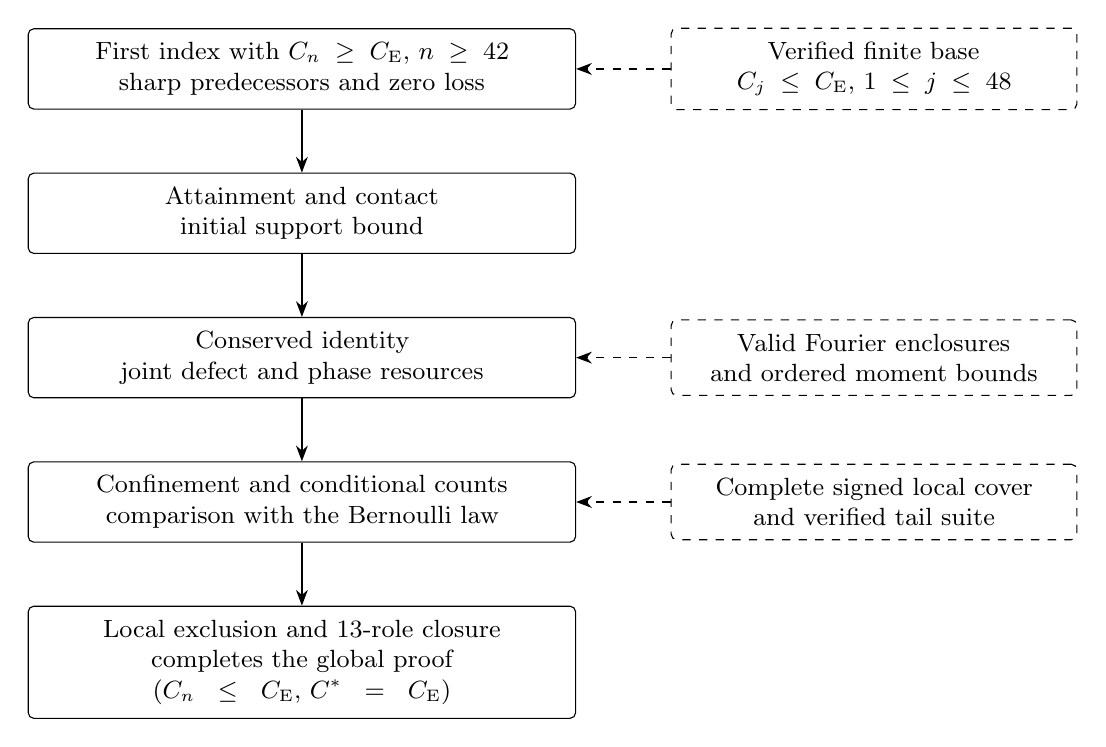
\begin{tikzpicture}[
 node distance=8mm,
 box/.style={draw,rounded corners=2pt,align=center,font=\small,
             text width=66mm,inner sep=5pt},
 input/.style={box,text width=48mm,dashed},
 arr/.style={-{Stealth[length=2mm]},semithick}]
\node[box] (entry) {First index with $C_n\ge\CE$, $n\ge42$\\
  sharp predecessors and zero loss};
\node[box,below=of entry] (contact) {Attainment and contact\\
  initial support bound};
\node[box,below=of contact] (resource) {Conserved identity\\
  joint defect and phase resources};
\node[box,below=of resource] (count) {Confinement and conditional counts\\
  comparison with the Bernoulli law};
\node[box,below=of count] (end) {Local exclusion and 13-role closure\\
  completes the global proof ($C_n\le\CE$, $C^*=\CE$)};
\node[input,right=12mm of entry] (base) {Verified finite base\\
  $C_j\le\CE$, $1\le j\le48$};
\node[input,right=12mm of resource] (fourier) {Valid Fourier enclosures\\
  and ordered moment bounds};
\node[input,right=12mm of count] (local) {Complete signed local cover\\
  and verified tail suite};
\draw[arr] (entry)--(contact);
\draw[arr] (contact)--(resource);
\draw[arr] (resource)--(count);
\draw[arr] (count)--(end);
\draw[arr,dashed] (base)--(entry);
\draw[arr,dashed] (fourier)--(resource);
\draw[arr,dashed] (local)--(count);
\end{tikzpicture}
\caption{The route to the local exclusion and global closure. Dashed boxes show
the certificate inputs; their completed \texttt{full\_pass} verification is
recorded in Section~\ref{ms:certificates}.}
\label{ms:fig:dependencies}
\end{figure}

\subsection{Notation and reading order}\label{ms:notation}
The main variables are listed below. Auxiliary variables used only in a
single estimate are defined where they occur.
\begin{center}\small
\begin{tabular}{@{}lP{110mm}@{}}\toprule
Symbol & Meaning\\\midrule
$H$, $z=H/\sqrt n$ & Raw and standardized thresholds.\\
$p,q,m$ & Sign probabilities and common one-sided first moment.\\
$\rho,\gamma,\beta$ & $\E|X|^3$, $\E X^3$, and $\E[X|X|]$.\\
$\ell$ & Span between conditional means; $\ell=m/(pq)$.\\
$W$, $U=W/\ell$ & Physical and count-scale conditional noise.\\
$\theta$, $s$, $\lambda$ & $\E W^2$, $\E U^2$, and $ns$; $\theta=s/(pq+s)$.\\
$D$, $d_n$, $d_Y$ & Moment defect, predecessor score decrement, and inward count-gap displacement.\\
$k,u$ & Nearest integer count and phase: $np+H/\ell=k+u$, $|u|\le1/2$.\\
$\sigma=\sqrt{10}$ & Constant in the defect decomposition.\\\bottomrule
\end{tabular}
\end{center}

Sections~\ref{ms:extremizers}--\ref{ms:counts} contain the analytic
argument, and Section~\ref{ms:certificates} the main global theorem
and the \texttt{full\_pass} verification of the thirteen certificate roles. The appendices contain the
longer Fourier estimates, the finite-index arguments and the explicit
comparison formulas.

\input{sections/02-extremizers}
\input{sections/02b-moment-domain}
\input{sections/03-smoothing}
\input{sections/04-support}
\input{sections/05-geometry-counts}
\input{sections/05b-conserved}
\input{sections/06-resources}
\input{sections/05c-counts}
\input{sections/07-curvature}
\section{Certificate conditions, global composition, and full-pass verification}\label{ms:certificates}

This section states the main global theorem, explains what a
finite certificate must establish, and records the completed end-to-end
verification (\texttt{full\_pass: "ESTABLISHED"}) of all thirteen certificate
roles.

\subsection{The mathematical interface}

Write $a_n=C_n-\CE$ and
$d_n=n(C_{n-1}-C_n)_+$.

\begin{assumption}[Finite base]\label{ms:base41}
For every integer $1\le j\le41$, one has $C_j\le\CE$.
This must be proved without using Assumption~\ref{ms:local42}.
\end{assumption}

\begin{assumption}[Equality-inclusive local exclusion]\label{ms:local42}
For every integer $n\ge42$, the following conditions do not hold
simultaneously:
\begin{equation}\label{ms:local-entry}
 \begin{gathered}
 0\le n(C_n-\CE)\le0.54,\qquad d_n=0,\qquad C_n<0.4226,\\
 C_{n-1}<0.4253,\qquad C_{n-2}<0.4253.
 \end{gathered}
\end{equation}
Since $C_n$ is attained (Lemma~\ref{ms:attainment}), this is equivalent to
the nonexistence of an extremal pair at index $n$ under these conditions.
\end{assumption}

The proof of the local exclusion combines the analytic results of
Sections~\ref{ms:support}--\ref{ms:counts} with finite certificates, in
four stages. First, the contact inequality and the moment
bounds give the initial support interval. Second, an ordered sequence of
Fourier estimates, moment intersections and support contractions gives
one closed parameter panel containing the maximizing law. Third, a joint
defect inequality and a confinement argument bound its conditional noise
and its support near the two-point skeleton. Fourth, the exact
conditional-count representation gives a comparison on every remaining
closed phase and noise cell. The analytic steps are in Sections~\ref{ms:support}--\ref{ms:counts}
and the appendices; their numerical inputs and all thirteen finite and
effective-tail roles have been verified end-to-end in the public release.

The stages are applied in order to one fixed extremal pair: each support
contraction may use only moment bounds proved from the preceding support
interval, and the deleted sums $S_{n-1}$ and $S_{n-2}$ are compared with
the Gaussian through the constants $C_{n-1}$ and $C_{n-2}$.

\begin{theorem}[Main all-index theorem: sharp iid Berry--Esseen constant]\label{ms:conditional-global}
Suppose Assumptions~\ref{ms:base41} and~\ref{ms:local42} hold. Then
\[
 C_n<\CE\quad(n\ge42),\qquad C^*=\CE.
\]
Moreover, the analytic reductions proved in Sections~\ref{ms:extremizers}--\ref{ms:counts}
and the appendices, combined with the verified thirteen-role exact certificate
partition covering $1\le n\le48$ and $n\ge49$ (Table~\ref{ms:tab:roles}),
establish unconditionally that for every integer $n\ge1$,
\[
 C_n\le\CE\quad(n\ge1),\qquad C^*=\sup_{n\ge1}C_n=\CE=\frac{3+\sqrt{10}}{6\sqrt{2\pi}}.
\]
\end{theorem}
\begin{proof}
Under Assumptions~\ref{ms:base41} and~\ref{ms:local42}, if the strict tail
conclusion fails, choose the least $n\ge42$ with $C_n\ge\CE$. Both
predecessors are at most $\CE$: at $n=42$ these are
exactly the base indices $40$ and $41$. Hence $d_n=0$ and the two
deleted caps in~\eqref{ms:local-entry} hold. The smoothing recurrence
of Section~\ref{ms:smoothing} gives
\[
 0\le n(C_n-\CE)<\frac{3003}{10250}<0.3,
 \qquad C_n<\frac{73}{175}<0.4226.
\]
Thus all conditions in~\eqref{ms:local-entry} hold, contradicting
Assumption~\ref{ms:local42}.

In the verified thirteen-role partition (Table~\ref{ms:tab:roles}),
the small-index foundations establish $C_1\le2/5<\CE$ (\texttt{N1}),
$C_2\le2\sqrt2/7<\CE$ (\texttt{G2}), $C_3\le59\sqrt3/250<\CE$ (\texttt{G3}),
and $C_4\le0.4097<\CE$ (\texttt{ROOT4}); sequential same-law weak-predecessor
induction closes $n=5$ (\texttt{C5-one-free}), $6\le n\le9$
(\texttt{projected-C69}), $10\le n\le19$ (\texttt{projected-C1019}),
$20\le n\le24$ (\texttt{current-C2024}), $n=25$ (\texttt{current-C25}),
$26\le n\le39$ (\texttt{current-C2639}), and $40\le n\le42$
(\texttt{current-C4042}); the independent 183-task collector family closes
$43\le n\le48$ (\texttt{current-C4348}); and the 55-predicate effective-tail
suite (\texttt{independent-tail49}) establishes the three-loss base at
$49,48,47$ ($C_{46}>\CE+0.19(1/47+1/48+1/49)>\CE+0.54/46$, contradicting the
verified strong cap at $46$) and excludes the least later failure $n\ge50$.
Thus $C_n\le\CE$ for every $n\ge1$ and $C^*\le\CE$; the fixed Bernoulli limit
\eqref{ms:bernoulli-limit} gives $C^*\ge\CE$, hence $C^*=\CE$.
\end{proof}

If Assumption~\ref{ms:local42} is weakened to exclude only $C_n>\CE$, the
same argument, applied to the least $n$ with $C_n>\CE$, still gives
$C^*=\CE$.

\subsection{What a finite certificate must establish}

A certificate has three ingredients. Its domain
description contains every actual parameter tuple allowed by the
analytic hypotheses. Its local proof establishes the required inequality
throughout each closed cell. Its coverage proof shows that the cells
exhaust that domain.

The following elementary lemma is the basic tool for tensor certificates.

\begin{lemma}[Common-marginal expectation and score]
\label{ms:certificate-expectation}
Let $K\subset\R$ contain the support of $P\in\mathcal P$. Let
$f_0,\ldots,f_d$ be integrable functions under $P$, with $f_0=1$, and let
$m_j=\E f_j(X)$. For a finite tensor sum
\[
 T(x_1,\ldots,x_n)=\sum_{\alpha}t_\alpha
                              \prod_{i=1}^n f_{\alpha_i}(x_i),
\]
independence gives
\begin{equation}
 \E T(X_1,\ldots,X_n)=\sum_\alpha t_\alpha\prod_{i=1}^n m_{\alpha_i}.
\label{ms:tensor-expectation}
\end{equation}
If $T\ge\mathbf1_{\{x_1+\cdots+x_n\le H\}}$ on all of $K^n$ and
\[
 \sum_\alpha t_\alpha\prod_i m_{\alpha_i}
         -\Phi(H/\sqrt n)\le a\rho/\sqrt n,
\]
then $\Pp(S_n\le H)-\Phi(H/\sqrt n)\le a\rho/\sqrt n$.
\end{lemma}
\begin{proof}
Each product is absolutely integrable, because independence factors its
absolute expectation into the finite quantities $\E|f_j(X)|$.
Fubini and linearity prove \eqref{ms:tensor-expectation}. Integrate the
pointwise majorant and use $\rho>0$ to obtain the score inequality.

\end{proof}

For example, a tensor product containing a centered factor has zero
expectation when all other factors concern different independent variables.
Such terms may improve a pointwise majorant without altering its expectation.
Polynomial factors of degree above three require the corresponding moments.
For the extremal laws used here, these are finite because support is compact.

An exact polynomial positivity certificate often uses Bernstein coefficients.
On $[0,1]$, set $B_{j,d}(t)=\binom dj t^j(1-t)^{d-j}$. They are
nonnegative and sum to one. The identity
\[
 t^k=\sum_{j=k}^d\frac{\binom jk}{\binom dk}B_{j,d}(t)
\]
follows from
$\binom dj\binom jk=\binom dk\binom{d-k}{j-k}$ and the binomial theorem.
Applying it in each coordinate proves that a polynomial
$\sum_\alpha a_\alpha t^\alpha$ of coordinate degrees at most $d_i$ has
tensor Bernstein coefficients
\[
 b_\nu=\sum_{\alpha\le\nu}a_\alpha
                      \prod_i\frac{\binom{\nu_i}{\alpha_i}}
                                      {\binom{d_i}{\alpha_i}}.
\]
Thus nonnegative coefficients prove nonnegativity on the whole closed box.
For $P(x)=\sum_{i=0}^d a_i x^i$ on $[l,h]$, the change
$x=l+(h-l)t$ gives power coefficients
$\widetilde a_j=(h-l)^j\sum_{i=j}^d a_i\binom ij l^{i-j}$.
Applying the preceding identity gives the Bernstein coefficients on that
interval. Rational affine changes and subdivision preserve exactness. A certificate must also verify the polynomial identity and the coverage
of the domain.

The event plane needs particular care. On the closed side
$\sum x_i\le H$ the required inequality is $T-1\ge0$; on the other side
it is $T\ge0$. A certificate which verifies only $T\ge0$ at a boundary
point has not proved the closed-event majorant there. Sign orthants,
event-plane intersections and endpoint atoms must be included in the
pointwise proof.

\begin{proposition}[Closed-cover soundness]
\label{ms:closed-cover}
Suppose a family of actual laws and thresholds has an analytically proved
map into a covered parameter domain. A finite certificate has finitely
many roots covering that domain and a finite subdivision tree at each
root. Every split retains both closed children. At each leaf, either
a proved necessary condition excludes every actual mapped point in the
leaf, or a valid whole-leaf inequality bounds its positive score by $a$.
Then all actual points in the root domain have positive score at most $a$.
If every leaf instead excludes a putative attained score $C\ge\CE$, no
such attained witness belongs to the root domain.
\end{proposition}
\begin{proof}
An actual point at a parent belongs to at least one child, including if it
lies on the common boundary. Induction up each finite tree transfers the
leaf conclusion to its root. The root union transfers it to the complete
mapped domain. In the second version no actual point can lie in any leaf, a
contradiction.
\end{proof}

A root may describe a relaxation containing parameters of no actual law;
this does not affect soundness, whereas a missing root or an unfinished
subdivision does. A minimum of convex bounds need not be convex, so an
endpoint maximization must be justified for each bound before the minimum
is taken.

In interval computations every transcendental function is enclosed
outwards and every denominator is proved positive on the whole cell; a
lower bound for a binomial mass multiplies a bracket only after the
bracket is known to be negative.

A cover must include both signs of the phase, all admissible nearest
counts, the endpoints of probability panels and the boundaries between
noise bands. The case $\lambda=n\E U^2=0$ is separate: then $U=0$ almost
surely, the law is a two-point law, and Schulz's theorem
applies~\cite{Schulz2016}.

\subsection{Verified thirteen-role partition and full-pass completion}

Sections~\ref{ms:extremizers}--\ref{ms:counts} and the appendices prove the
analytic implications, with their moment, support and remainder hypotheses.
All thirteen finite-index and effective-tail certificate families have now been
verified end-to-end in the public verification release
(\texttt{full\_pass: "ESTABLISHED"}, \texttt{public\_verification: "FULL\_PASS\_VERIFIED"},
zero remaining obligations). Table~\ref{ms:tab:roles} summarizes the thirteen
verified roles covering every integer $n\ge1$.

\begin{center}\small
\begin{longtable}{@{}P{0.10\textwidth}P{0.44\textwidth}P{0.38\textwidth}@{}}
\caption{Complete thirteen-role verified partition covering all $n\ge1$.}
\label{ms:tab:roles}\\\toprule
Index & Mathematical role & Verified certificate receipt\\\midrule
\endfirsthead\toprule
Index & Mathematical role & Verified certificate receipt\\\midrule\endhead
$1$ & $C_1\le2/5<\CE$ via cubic-dual majorants (\texttt{N1}). & 150 closed cells, 1,128 Bernstein intervals (\texttt{03ed6774681f}).\\
$2$ & $C_2\le2\sqrt2/7<\CE$, tensor reduction (\texttt{G2}). & 70/70 primary and 70/70 independent polynomial cells.\\
$3$ & $C_3\le59\sqrt3/250<\CE$, 59-feature null polynomial (\texttt{G3}). & 95,904 grid identities and 111/111 C++ cube checks.\\
$4$ & $C_4\le0.4097<\CE$ from quantitative $G_3$ (\texttt{G4/ROOT4}). & Complete two-pass 260-geometry, 1,300 HIGH-slot closure.\\
$5$ & One-free $G_3\to G_4\to$ same-owner $q_5=0$ exclusion (\texttt{C5-one-free}). & Complete region/resource/COUNT cover, 13 rules.\\
$6$--$9$ & Same-law induction from weak $C_5$ parent (\texttt{projected-C69}). & Complete original resource/COUNT contexts.\\
$10$--$19$ & Parent substitution from the $6$--$9$ theorem (\texttt{projected-C1019}). & Complete resource/COUNT contexts and subdomains.\\
$20$--$24$ & Increasing weak induction, own caps $<0.419$ (\texttt{current-C2024}). & 49 \texttt{actual20} + 114 public COUNTs, 186 meanings, 1,000 panels.\\
$25$ & Low-only $[1,6/5]$ cover + high-$\rho$ branch (\texttt{current-C25}). & 6 original calls, 52 complete COUNT interfaces.\\
$26$--$39$ & Low-only weak induction; support35 and positive39 cap (\texttt{current-C2639}). & 300 COUNTs, whole7 partitions, 35 support predicates.\\
$40$--$42$ & Weighted floor40 theorem for $n\in\{40,41,42\}$ (\texttt{current-C4042}). & CORE304 + 2/9/INITIAL2 acquisition conjunction.\\
$43$--$48$ & Independent positive ceilings and finite least failure (\texttt{current-C4348}). & 183/183 tasks + \texttt{collector43}, \texttt{collector44} (\texttt{bed1a5933ce0}).\\
$n\ge49$ & Three-loss base at $49,48,47$ and least later failure (\texttt{independent-tail49}). & 14 top-level + 41 retained execution predicates (\texttt{55b2be8e21f1}).\\\bottomrule
\end{longtable}
\end{center}

In total, the verified public release records 1,243/1,243 passed public
\texttt{COUNT} jobs (SHA-256 prefix \texttt{9eaa11eb6ab8}), 49/49 passed
\texttt{actual20} \texttt{COUNT} jobs and their mathematical namespace bridge
(\texttt{d522d7477749}) plus 5 scalar contracts, all 7 foundation stages
(\texttt{G2}, \texttt{G3}, and \texttt{ROOT4} two-pass), all 183/183 native
\texttt{finite43-48} tasks and both collectors, all 55/55 native
\texttt{tail49} predicates, and the global composition proof objects
\texttt{upper/PROOF.json} (\texttt{5acc019642ae}), \texttt{lower/PROOF.json}
(\texttt{018bdf1b6918}), and \texttt{equality/PROOF.json}
(\texttt{8be2f7c6083d}). Running \texttt{python -I -B be.py status} and
\texttt{python -I -B be.py verify} verifies the complete release with
\texttt{EXIT\_CODE=0}.

\begin{center}
\begin{tabular}{@{}P{0.36\textwidth}P{0.30\textwidth}P{0.27\textwidth}@{}}
\toprule
Result & Mathematical status & Computation status\\
\midrule
Attainment, contact and smoothing & Proved for the stated class of laws &
Verified (\texttt{EXIT\_CODE=0})\\[3pt]
Support, conserved identity, score charge and curvature & Proved under the
stated hypotheses & Exact algebra and bounded arithmetic verified\\[3pt]
Complete Fourier, confinement and finite-index chain & Proved and audited across
all 13 roles & Full end-to-end replay verified\\[3pt]
All-index bound $C_n\le\CE$ ($n\ge1$) and $C^*=\CE$ & Proved unconditionally &
\texttt{full\_pass: "ESTABLISHED"}\\
\bottomrule
\end{tabular}
\end{center}

\section{Discussion}\label{ms:discussion}

Combining the analytic reductions with the verified thirteen-role certificate
family establishes $C_n\le\CE$ for every integer $n\ge1$ and $C^*=\CE$
unconditionally (\texttt{full\_pass: "ESTABLISHED"}). The induction needs no
astronomically large terminal index: at the first failure index beyond the
finite base, the deleted predecessors are already controlled, and the
three-loss base at $49,48,47$ together with the uniform first-failure argument
closes the entire unbounded tail.

The most delicate part of the local exclusion is the comparison near the
two-point law. An absolute error of order $n^{-3/2}$ is not small compared
with an arbitrarily small defect, so the estimates must be relative to the
conditional noise $\lambda$. The exact count identities of
Section~\ref{ms:counts} are designed for this purpose; the uniform
relative bounds they require are verified across all noise and phase cells in
the public certificate suite.

\subsection*{Use of artificial intelligence}

AI systems were used extensively in the research, verification, and preparation
of this manuscript. ChatGPT, Codex, and Gemini/Antigravity assisted with
mathematical exploration, programs for exact checks, distributed cloud
verification of the full certificate family, source and bibliography
comparisons, and drafting and revising the exposition. The authors take
responsibility for the mathematical content and presentation.

The work builds in part on an earlier AI-assisted draft deposited on
Hexagon~\cite{rodziewiczkolodziejek2026momentdefects}. The present paper
reorganizes that material, develops the analytic reductions above, and reports
the completed end-to-end verification (\texttt{full\_pass: "ESTABLISHED"}) in
Section~\ref{ms:certificates}.

\subsection*{Code and data}

The certificates, the verification receipts, the programs that check them, and
the source of this paper are available at
\url{https://github.com/kolodziejek/berry-esseen-certificates} and
\url{https://github.com/rodziewiczk/berry-esseen-certificates}.

\appendix
\setcounter{secnumdepth}{4}
\section{Half-line smoothing, characteristic functions, and resource enclosures}
\label{ms:fourier:appendix}

\subsection{Exact half-line smoothing}
\label{ms:fourier:kernel}

The main conserved identity reduces the problem to bounding explicit
Fourier integrals and moment expressions. This appendix develops the
half-line smoothing kernel, characteristic-function enclosures, complete
low- and high-frequency bounds, and the resource-to-confinement maps
used in those estimates. Section~\ref{ms:certificates} records their
certificate conditions and verification status.

Write $\phi$ and $\Phi$ for the standard normal density and distribution
function. All terminating decimals are exact rational numbers. The
imaginary unit is $i$. Symbols introduced within a subsection, including
$D$, $R$, $L$, $s$ and $K$, are local to that subsection unless explicitly
carried forward. In particular the moment defect $D$, an auxiliary distance
bound, and the Bernoulli inward displacement $d$ are different quantities.

The one-sided kernel is
\[
 K(t)=\frac{1-t}{2}+\frac{i}{2}
       \left((1-t)\cot(\pi t)+\frac1\pi\right),\qquad 0<t<1.
\]
For $\kappa\in\{K,\overline K\}$, $0<b\le1$ and
$g(t)=g(0)+O(t)$ with real $g(0)$, the convention throughout is
\begin{equation}\label{ms:fourier:kernel-convention}
 \mathfrak I_{\kappa,b}(g)
 =2\lim_{\epsilon\downarrow0}\operatorname{Re}
       \int_\epsilon^b\kappa(t)g(t)\,dt.
\end{equation}
Only the real-part improper limit is intended; the unmodified complex
integral need not converge. The proof below establishes directly that
\[
 M(x)=\tfrac12+\mathfrak I_{K,1}(e^{2\pi itx})
       \ge\mathbf1_{(-\infty,0]}(x),\qquad
 1-M(-x)\le\mathbf1_{(-\infty,0)}(x),
\]
including atoms at the boundary, and justifies the expectation identity
for an integrable random variable.

\subsubsection{A real-variable Beurling construction}

Set

\[
 W(x)=\left(\frac{\sin\pi x}{\pi x}\right)^2\quad(x\ne0),
 \qquad W(0)=1,
\]

and define the continuous odd function

\begin{equation}
 H_B(x)=\sum_{m=1}^{\infty}\{W(x-m)-W(x+m)\}+2xW(x).
 \label{ms:fourier:kernel-1}
\end{equation}

The series converges absolutely and locally uniformly on the real line:
for \(|x|\le R\) and \(m>2R+1\), each shifted term is bounded by a
constant times \(m^{-2}\). Thus the function and all the integer values in
what follows are unambiguous. In particular,

\begin{equation}
 H_B(0)=0,\qquad H_B(j)=\operatorname{sgn}(j)
 \quad(j\in\mathbb Z\setminus\{0\}).                 \label{ms:fourier:kernel-2}
\end{equation}

Here \(\operatorname{sgn}(0)=0\). The corresponding classical Beurling
majorant is \(B=H_B+W\). For noninteger \(x\), its series is

\begin{equation}
 B(x)=\left(\frac{\sin\pi x}{\pi}\right)^2
 \left\{\frac2x+\sum_{m=0}^{\infty}\frac1{(x-m)^2}
                    -\sum_{m=1}^{\infty}\frac1{(x+m)^2}\right\}.
 \label{ms:fourier:kernel-3}
\end{equation}

We prove the needed inequality directly, without importing an extremality
or Fourier-transform theorem about \(B\).

The elementary partial-fraction identity

\begin{equation}
 \sum_{m\in\mathbb Z}\frac1{(y-m)^2}
       =\frac{\pi^2}{\sin^2\pi y},\qquad y\notin\mathbb Z,
 \label{ms:fourier:kernel-4}
\end{equation}

has the following short proof. Integrate
\(\pi\cot(\pi z)/(z-y)^2\) counterclockwise over the square with vertices
\(\pm(N+\tfrac12)\pm i(N+\tfrac12)\). The cotangent is uniformly bounded
on these edges: on the vertical edges it is a multiple of a hyperbolic
tangent, and on the horizontal edges its modulus is bounded by
\(\coth(\pi(N+\tfrac12))\). The denominator is of order \(N^2\) and the
perimeter of order \(N\), so the integral tends to zero. Its residues are
\((m-y)^{-2}\) at \(m=-N,\ldots,N\), and
\(-\pi^2\csc^2(\pi y)\) at \(y\). The residue theorem and absolute
convergence give \eqref{ms:fourier:kernel-4}.

For \(y>0\), \(y\notin\mathbb Z\), put

\[
 A(y)=\left(\frac{\sin\pi y}{\pi}\right)^2,
 \qquad S(y)=\sum_{m=1}^{\infty}(y+m)^{-2}.
\]

Subtracting \eqref{ms:fourier:kernel-4} from \eqref{ms:fourier:kernel-1} gives exactly

\begin{equation}
 H_B(y)-1=A(y)\left\{\frac2y-\frac1{y^2}-2S(y)\right\}.
 \label{ms:fourier:kernel-5}
\end{equation}

The decreasing positive function \(s\mapsto(y+s)^{-2}\) satisfies

\begin{equation}
 S(y)\le\int_0^\infty(y+s)^{-2}\,ds=\frac1y
       \le\frac1{y^2}+S(y).
 \label{ms:fourier:kernel-6}
\end{equation}

Consequently the expression in braces in \eqref{ms:fourier:kernel-5} lies between
\(-y^{-2}\) and \(y^{-2}\). Hence

\[
 |H_B(y)-1|\le W(y)\quad(y>0).
\]

Positive integer points follow directly from \eqref{ms:fourier:kernel-2}. Oddness of \(H_B\) and
evenness of \(W\), together with their values at zero, now prove

\begin{equation}
 |H_B(x)-\operatorname{sgn}(x)|\le W(x)
 \qquad(x\in\mathbb R).                              \label{ms:fourier:kernel-7}
\end{equation}

This is the required sign-function majorization, with its normalization
proved rather than assumed.

\subsubsection{Recovering the exact Fourier kernel}

Elementary integration gives, for every real \(x\),

\begin{equation}
 W(x)=2\int_0^1(1-t)\cos(2\pi tx)\,dt.              \label{ms:fourier:kernel-8}
\end{equation}

For \(0<r<1\), insert \eqref{ms:fourier:kernel-8} into the absolutely convergent Abel-weighted
series. Termwise integration is legitimate because
\(\sum_{m\ge1}r^m<\infty\). The cosine subtraction formula gives

\begin{equation}
 \begin{aligned}
 \sum_{m\ge1}r^m\{W(x-m)-W(x+m)\}
   &=4\int_0^1(1-t)\sin(2\pi tx)
               \sum_{m\ge1}r^m\sin(2\pi mt)\,dt\\
   &=4\int_0^1(1-t)\sin(2\pi tx)
        \frac{r\sin(2\pi t)}{1-2r\cos(2\pi t)+r^2}\,dt.
 \end{aligned}                                                    \label{ms:fourier:kernel-9}
\end{equation}

For \(0<t<1\),

\begin{equation}
 \left|\frac{r\sin(2\pi t)}{1-2r\cos(2\pi t)+r^2}\right|
 \le\frac12|\cot(\pi t)|,
 \label{ms:fourier:kernel-10}
\end{equation}

since the denominator is
\((1-r)^2+4r\sin^2(\pi t)\). The right side of \eqref{ms:fourier:kernel-9}, including its
remaining factors, is therefore dominated by

\[
 2(1-t)|\sin(2\pi tx)|\,|\cot(\pi t)|.
\]

This is integrable at both endpoints: the sine is \(O_x(t)\) at zero,
and \((1-t)\cot(\pi t)\) is bounded at one. Dominated convergence on
the integral side and absolute convergence on the series side allow
\(r\uparrow1\). The fraction in \eqref{ms:fourier:kernel-9} tends to
\(\tfrac12\cot(\pi t)\). Also, direct integration gives

\begin{equation}
 2xW(x)=\frac2\pi\int_0^1\sin(2\pi tx)\,dt,          \label{ms:fourier:kernel-11}
\end{equation}

including \(x=0\). Combining \eqref{ms:fourier:kernel-1} and \eqref{ms:fourier:kernel-9}--\eqref{ms:fourier:kernel-11},

\begin{equation}
 H_B(x)=2\int_0^1 R(t)\sin(2\pi tx)\,dt,
 \qquad R(t)=(1-t)\cot(\pi t)+\frac1\pi.
 \label{ms:fourier:kernel-12}
\end{equation}

Every integral in \eqref{ms:fourier:kernel-12} is a convergent real integral. No principal-value
Fourier manipulation has been used.

Now take exactly the manuscript's kernel

\begin{equation}
 K(t)=\frac{1-t}{2}+\frac i2 R(t),\qquad0<t<1.
 \label{ms:fourier:kernel-13}
\end{equation}

Equations \eqref{ms:fourier:kernel-8} and \eqref{ms:fourier:kernel-12} establish the exact identity

\begin{equation}
 \boxed{\displaystyle
 M(x):=\frac12+2\lim_{\epsilon\downarrow0}\operatorname{Re}
       \int_\epsilon^1K(t)e^{2\pi itx}\,dt
       =\frac{1-H_B(x)+W(x)}2=\frac{1+B(-x)}2.}
 \label{ms:fourier:kernel-14}
\end{equation}

In particular, the exponent has the \emph{positive} sign and the imaginary
part of \(K\) has the \emph{positive} sign. The minus sign on \(H_B\) comes
from taking the real part of \(iR(t)e^{2\pi itx}\).

\subsubsection{Closed boundary, cardinal values and the minorant}

For \(x<0\), \eqref{ms:fourier:kernel-7} gives \(M(x)\ge1\); for \(x>0\), it gives
\(M(x)\ge0\). At the boundary, \eqref{ms:fourier:kernel-2} and \(W(0)=1\) give

\begin{equation}
 M(0)=1.                                             \label{ms:fourier:kernel-15}
\end{equation}

Thus this majorizes the \emph{closed} half-line, including a point mass at
zero, rather than merely the half-height convention for a jump:

\begin{equation}
 M(x)\ge1_{(-\infty,0]}(x),\qquad
 1-M(-x)\le1_{(-\infty,0)}(x).
 \label{ms:fourier:kernel-16}
\end{equation}

The second inequality follows by subtracting the first inequality at
\(-x\) from one; its endpoint is open. Direct cardinal values are

\begin{equation}
 M(j)=1_{\{j\le0\}},\qquad1-M(-j)=1_{\{j<0\}}
 \quad(j\in\mathbb Z).                              \label{ms:fourier:kernel-17}
\end{equation}

The proof also gives the useful global error bound

\begin{equation}
 0\le M(x)-1_{(-\infty,0]}(x)\le W(x)
 \quad(x\in\mathbb R).                              \label{ms:fourier:kernel-18}
\end{equation}

At zero the left-hand error is exactly zero; it is not obtained by
assigning half of an atom to each side. In particular \(0\le M\le2\).

\subsubsection{Expectations and the compensated identity}

Suppose \(U\) is real and \(\E|U|<\infty\), and use the convention
\(\psi_U(t)=\E e^{2\pi itU}\). Since
\(2\int_0^1\operatorname{Re}K(t)\,dt=1/2\), \eqref{ms:fourier:kernel-14} can be written

\begin{equation}
 M(u)=1+2\operatorname{Re}\int_0^1
             K(t)\{e^{2\pi itu}-1\}\,dt.             \label{ms:fourier:kernel-19}
\end{equation}

The complex integral in \eqref{ms:fourier:kernel-19} is absolutely convergent. Indeed,
\(K(t)=i/(2\pi t)+1/2+O(t)\) at zero, \(K\) is bounded near one,
and

\[
 \E|e^{2\pi itU}-1|\le2\pi t\,\E|U|.
\]

Consequently
\(\int_0^1|K(t)|\E|e^{2\pi itU}-1|\,dt<\infty\), so ordinary
absolute Fubini applies to \eqref{ms:fourier:kernel-19}. Restoring the constant real part gives

\begin{equation}
 \E M(U)=\frac12+
     2\lim_{\epsilon\downarrow0}\operatorname{Re}
        \int_\epsilon^1K(t)\psi_U(t)\,dt.            \label{ms:fourier:kernel-20}
\end{equation}

Since \(\psi_{-U}=\overline{\psi_U}\), conjugation similarly yields

\begin{equation}
 \E\{1-M(-U)\}=\frac12-
     2\lim_{\epsilon\downarrow0}\operatorname{Re}
        \int_\epsilon^1\overline{K(t)}\psi_U(t)\,dt.
 \label{ms:fourier:kernel-21}
\end{equation}

These are the two expectation identities under the real-part
improper convention \eqref{ms:fourier:kernel-convention}. All expectations are finite; \eqref{ms:fourier:kernel-18} even gives
boundedness of the majorant without a moment assumption. The first
absolute moment is a sufficient hypothesis for the stated compensated
Fourier/Fubini argument. The uncompensated complex integral itself need
not converge.

\subsubsection{Four-summand smoothing normalization}

Let \(Y\) be integrable, let \(h\in\mathbb R\), and let \(T>0\). For
\(\chi_Y(s)=\E e^{isY}\), apply \eqref{ms:fourier:kernel-16} and \eqref{ms:fourier:kernel-20} to
\(U=T(Y-h)/(2\pi)\). The resulting exact normalization is

\begin{equation}
 \Pp(Y\le h)\le\frac12+
  2\lim_{\epsilon\downarrow0}\operatorname{Re}
       \int_\epsilon^1K(t)e^{-iTth}\chi_Y(Tt)\,dt.
 \label{ms:fourier:kernel-22}
\end{equation}

For the four-summand application,
\(Z=(X_1+\cdots+X_4)/2\), \(\varphi_P(s)=\E e^{isX_1}\),
and iid summands, choose \(T=6\). Independence gives
\(\chi_Z(6t)=\varphi_P(3t)^4\). Thus \eqref{ms:fourier:kernel-22} is exactly

\begin{equation}
 F_Z(x)\le\frac12+\int_0^1\operatorname{Re}
   \{\widehat K(t)e^{-6itx}\varphi_P(3t)^4\}\,dt,
 \qquad \widehat K=2K,
 \label{ms:fourier:kernel-23}
\end{equation}

the physical four-summand smoothing normalization. Writing \(D=x-Z\) and
\(S(t)=tR(t)\), its real integrand is exactly

\begin{equation}
 (1-t)\E\cos(6Dt)+S(t)\E[6D\operatorname{sinc}(6Dt)],
 \qquad \operatorname{sinc}(v)=\sin(v)/v,
 \label{ms:fourier:kernel-24}
\end{equation}

with the continuous value at zero. This verifies both the factor six
and the sign of the sine term. No non-atomicity, finite-support, density,
or continuity-at-the-threshold assumption is needed. For \eqref{ms:fourier:kernel-23}, iid
independence and integrability are sufficient; the manuscript's bounded
support assumptions imply integrability.

\subsection{Characteristic functions and conserved resources}
\label{ms:fourier:resources}

The following arguments retain the actual marginal law and raw threshold.
Attainment and contact are inputs where explicitly stated; the numerical
support, moments and probability panels are acquired hypotheses. The
finite induction at the end justifies a declared schedule of valid
updates, not the acceptance of any particular schedule. The classical
four-term Prawitz smoothing inequality is explicitly cited at its use.
The preceding pointwise construction alone is not substituted for that
external inequality without deriving its four-term normalization.

\subsubsection{Elementary characteristic-function bounds}
\label{ms:fourier:afcore:sec:fourier}

Throughout this section, $X$ is real, $\E X=0$, $\E X^2=1$, and
$\rho=\E|X|^3<\infty$. Write
\[
 f(u)=\E e^{iuX},\qquad g(u)=e^{-u^2/2},\qquad \gamma=\E X^3.
\]
No support, extremality, or predecessor assumption is made here.

\paragraph{Real and imaginary coordinates}

\begin{lemma}[Anchored coordinates]\label{ms:fourier:afcore:lem:anchor}
For $0\le u\le\pi$,
\begin{align}
 \cos u\le\Re f(u)&\le\cos u+\frac{\rho-1}{6}u^3,
 \label{ms:fourier:afcore:eq:real-anchor}\\
 |\Im f(u)|^2&\le\frac{(\rho-1)(\rho+5/3)}{36}u^6.
 \label{ms:fourier:afcore:eq:imag-anchor}
\end{align}
\end{lemma}
\begin{proof}
Put $\operatorname{sinc}v=\int_0^1\cos(tv)\,dt$, including $v=0$.
The elementary bounds $|\sin v|\le|v|$ give
\[
 |\operatorname{sinc}a-\operatorname{sinc}b|
 \le\frac{|a-b|}{2},\qquad
 |\operatorname{sinc}a-\operatorname{sinc}b|
 \le\frac{|a^2-b^2|}{6}.
\]
For the second inequality, use
$|\cos\sqrt A-\cos\sqrt B|\le|A-B|/2$ for $A,B\ge0$,
and integrate in $t$. Evenness handles either sign of $a,b$.

For $r\ge0$, integration from $1$ to $r$ of the first sinc bound gives
\[
 \left|\cos(ur)-\cos u+
       \frac{u\sin u}{2}(r^2-1)\right|
 \le\frac{u^3}{12}(r-1)^2(2r+1).
\]
Indeed the derivative of the expression inside the absolute value is
$u^2r\{\operatorname{sinc}u-\operatorname{sinc}(ur)\}$, and
$\int_{\min(1,r)}^{\max(1,r)}t|t-1|\,dt
=(r-1)^2(2r+1)/6$.
For $R=|X|$, the weight $W(R)=(R-1)^2(2R+1)$ satisfies
$\E W(R)=2(\rho-1)$. Averaging proves the upper real bound, and in fact
the corresponding two-sided anchor error.

For the sharper lower bound, take $0<u\le\pi$ and
$a=\sin u/(2u)\ge0$. The function $v\mapsto\cos v+av^2$ has its
minimum on $[0,\pi]$ at $u$, since sinc decreases there. For $v\ge\pi$,
\[
 \cos v+av^2\ge-1+a\pi^2\ge\cos u+au^2.
\]
Thus this minimum is global on $[0,\infty)$. Substitute $v=uR$ and
average; $\E R^2=1$ cancels the quadratic term. The case $u=0$ is immediate.

Centering and the second sinc bound give
\[
 |\Im f(u)|
 \le\frac{u^3}{6}\E[R|R^2-1|].
\]
Cauchy--Schwarz, with $W$ as above, yields
\[
 \{\E[R|R^2-1|]\}^2
 \le\E W(R)\,
       \E\frac{R^2(R+1)^2}{2R+1}.
\]
There is no singularity at $R=1$: the factorization used here is
$R|R^2-1|=\sqrt{W(R)}R(R+1)/\sqrt{2R+1}$.
The identity
\[
 r^3+\frac{29r^2+1}{18}
 -\frac{2r^2(r+1)^2}{2r+1}
 =\frac{(r-1)^2(4r+1)}{18(2r+1)}\ge0
\]
shows that the second expectation is at most $(\rho+5/3)/2$.
This proves \eqref{ms:fourier:afcore:eq:imag-anchor}. Every expectation used is
finite under the third-moment assumption.
\end{proof}

\begin{lemma}[The sine circle]\label{ms:fourier:afcore:lem:sine-circle}
Let
\[
 r=\E X_+=\E X_->0,\quad A=\E X_+^2,\quad B=\E X_-^2,
 \qquad \zeta=\frac{2AB}{r}.
\]
Then $A+B=1$ and
\begin{equation}\label{ms:fourier:afcore:eq:sine-circle}
 \zeta^2+\frac{36|\Im f(u)|^2}{u^6}\le\rho^2
 \qquad(u\ne0),\qquad
 \zeta\ge b(\rho):=\frac{\sqrt{\rho^2+8}-\rho}{2}.
\end{equation}
In particular, for $0\le u\le\pi$ the coefficient in the imaginary
bound may be replaced by
\[
 |\Im f(u)|^2\le\frac{u^6}{36}
 \min\{(\rho-1)(\rho+5/3),\,\rho^2-b(\rho)^2\}.
\]
Both bounds also hold for $\gamma^2$ after deleting $u^6/36$.
\end{lemma}
\begin{proof}
Let $\mu_+,\mu_-$ be the restrictions of the law of $|X|$ to the
strictly positive and strictly negative classes, respectively. For
$a,b>0$, let $P_{a,b}$ put masses $b/(a+b),a/(a+b)$ at $a,-b$.
The measure
\[
 d\nu(a,b)=\frac{a+b}{r}\,d\mu_+(a)d\mu_-(b)
\]
has mass $\Pp(X\ne0)$. Mixing $P_{a,b}$ against $\nu$, and retaining
the original atom at zero, recovers the law of $X$.
For a component, write $f_{a,b}(u)=\E_{P_{a,b}}e^{iuX}$ and
\[
 e_{a,b}=\frac{2a^2b^2}{a+b},\qquad
 \rho_{a,b}=\frac{ab(a^2+b^2)}{a+b}.
\]
The squared-argument sinc bound gives
\[
 \left|\frac{6\Im f_{a,b}(u)}{u^3}\right|
 \le\frac{ab|a^2-b^2|}{a+b}.
\]
Consequently the Euclidean norm of
$(e_{a,b},6\Im f_{a,b}(u)/u^3)$ is at most $\rho_{a,b}$.
Integrate this vector inequality. The two integrals on the right and
in the first coordinate are $\rho$ and $2AB/r$, respectively.
The triangle inequality proves the circle. This argument also covers
an atom at zero, whose vector contribution is zero.

Signwise Cauchy inequalities give
\[
 A^2\le r\E X_+^3,\qquad B^2\le r\E X_-^3,\qquad
 \frac{r^2}{A}+\frac{r^2}{B}\le\Pp(X\ne0)\le1.
\]
Hence $\rho+\zeta\ge1/r$, $AB\ge r^2$ and $\zeta\ge2r$.
All quantities are positive, so
$\zeta(\rho+\zeta)\ge2$. Solving this quadratic gives the stated
lower bound. Finally
$6\Im f(u)/u^3\longrightarrow-\gamma$ as $u\to0$ by dominated
convergence, using $|\sin v-v|\le|v|^3/6$. This also proves the assertions
about $\gamma$.
\end{proof}

On a closed moment band $\rho\in[\rho_-,\rho_+]$, any rational $Z>0$
satisfying $Z^2+\rho_+Z\le2$ is a valid uniform lower bound for
$b(\rho)$. Thus no numerical square root is needed to certify this
part of the imaginary enclosure.

\paragraph{An explicit scalar certificate and its convex profile}

\begin{lemma}[Scalar cosine bound]\label{ms:fourier:afcore:lem:cosine}
Assume the finite Bernstein positivity condition specified in the proof
below. Then, for every real $x$,
\begin{equation}\label{ms:fourier:afcore:eq:cosine}
 \cos x\le1-\frac{x^2}{2}+\kappa|x|^3,
 \qquad \kappa=\frac{62}{625}.
\end{equation}
\end{lemma}
\begin{proof}
By evenness take $x\ge0$. For $x\ge T:=625/124$ the right side is
at least one. Let $P_{16}(x)=\sum_{j=0}^8(-1)^jx^{2j}/(2j)!$.
The sixteenth derivative of $\cos x-P_{16}(x)$ is $\cos x-1\le0$,
and its first sixteen initial data vanish. Therefore
$\cos x\le P_{16}(x)$ on the whole nonnegative half-line.
It remains to prove positivity on $[0,T]$ of
\[
 Q(x)=\frac{1-x^2/2+\kappa x^3-P_{16}(x)}{x^3}
      =\sum_{j=0}^{13}q_jx^j,
\]
where the removable value at zero is used and the exact coefficient
vector is
\begin{align*}
 (q_0,\ldots,q_6)&=
 \left(\frac{62}{625},-\frac1{24},0,\frac1{720},0,
 -\frac1{40320},0\right),\\
 (q_7,\ldots,q_{13})&=
 \left(\frac1{3628800},0,-\frac1{479001600},0,
 \frac1{87178291200},0,-\frac1{20922789888000}\right).
\end{align*}
Here is a fully specified finite rational certificate. For $0\le r<80$
set $(a_r,b_r)=(r/16,(r+1)/16)$, and set $(a_{80},b_{80})=(5,625/124)$.
For $0\le j,k\le13$ define
\begin{align}
 c_{r,j}&=\sum_{\ell=j}^{13}q_\ell\binom\ell j
               a_r^{\ell-j}(b_r-a_r)^j,\nonumber\\
 B_{r,k}&=\sum_{j=0}^k c_{r,j}\frac{\binom kj}{\binom{13}j}.
 \label{ms:fourier:afcore:eq:bernstein-data}
\end{align}
All $81\cdot14$ numbers are thereby specified without external data.
The finite arithmetic condition required here is
\begin{equation}\label{ms:fourier:afcore:eq:bernstein-min}
 \min_{0\le r\le80,\ 0\le k\le13}B_{r,k}
 =B_{63,12}=\frac{2479189}{65585520000}>0.
\end{equation}
The identity
\[
 Q(a_r+(b_r-a_r)t)
 =\sum_{k=0}^{13}B_{r,k}\binom{13}k t^k(1-t)^{13-k}
\]
follows by expanding either side. Its basis is nonnegative and sums
to one for $0\le t\le1$. Equations
\eqref{ms:fourier:afcore:eq:bernstein-data}--\eqref{ms:fourier:afcore:eq:bernstein-min}
therefore imply positivity on every entire closed cell when that finite
condition holds. The cells cover $[0,T]$, completing the conditional proof.
\end{proof}

\begin{lemma}[Compatible profile]\label{ms:fourier:afcore:lem:profile}
Put $c_{\cos}=1-\cos4$, $a=129/1250$ and $A=16a/c_{\cos}$. The function
\begin{equation}\label{ms:fourier:afcore:eq:profile}
 q(v)=\begin{cases}
  1/2-\kappa v,&0\le v\le4,\\
  A(1-\cos v)/v^2,&4\le v\le2\pi,\\
  0,&v\ge2\pi
 \end{cases}
\end{equation}
is continuous, nonnegative, convex and nonincreasing on $[0,\infty)$,
and $\cos v\le1-v^2q(v)$ there.
\end{lemma}
\begin{proof}
The scalar bound at four gives $c_{\cos}\ge16a>0$, hence $0<A\le1$.
The pieces agree at both endpoints. On the curved piece,
\[
 q'(v)=A\frac{v\sin v-2(1-\cos v)}{v^3}\le0,
 \qquad
 q''(v)=\frac{A}{v^4}
       \{6+(v^2-6)\cos v-4v\sin v\}.
\]
Write the brace as $B(v)$. On $[4,3\pi/2]$,
$B'(v)=-2v\cos v+(2-v^2)\sin v\ge0$.
The elementary bounds $25/8<\pi<22/7$ imply
$7\pi/6<4<3\pi/2$, so $B(4)\ge6-10+8=4$.
On $[3\pi/2,2\pi]$ each remaining term in $B$ is nonnegative,
and $B\ge6$. Thus the curved branch is convex, with derivative zero
at $2\pi$. The upward derivative join at four is equivalent to
\[
 258\sin4+119(1-\cos4)\ge0.
\]
Let $S_{15}(x)=\sum_{j=0}^7(-1)^jx^{2j+1}/(2j+1)!$.
The fifteenth derivative of $\sin x-S_{15}(x)$ is $1-\cos x\ge0$,
with vanishing initial data; hence $\sin x\ge S_{15}(x)$ for $x\ge0$.
The exact rational lower bound at the join is
\[
 258S_{15}(4)+119\{1-P_{16}(4)\}
 =\frac{967616288}{638512875}>1.
\]
This proves the required join. The profile majorizes the cosine defect
by the scalar inequality on $[0,4]$, by $A\le1$ on $[4,2\pi]$,
and by $\cos v\le1$ thereafter.

The bounds $25/8<\pi<22/7$ follow from the rational comparisons in
Lemma~\ref{ms:gaussian-constants}.
\end{proof}

\begin{lemma}[Whole-law modulus]\label{ms:fourier:afcore:lem:modulus}
Let $X'$ be an independent copy of $X$, and let
$D\ge\E|X-X'|^3/2$. For $u\ge0$,
\begin{equation}\label{ms:fourier:afcore:eq:modulus}
 |f(u)|^2\le1-2u^2q(uD).
\end{equation}
The universal choice $D=\rho+1$ is valid. In particular the two
nontrivial branches are
\[
 |f(u)|^2\le
 \begin{cases}
  1-u^2+2\kappa Du^3,&uD\le4,\\
  1-2A(1-\cos(uD))/D^2,&4\le uD\le2\pi.
 \end{cases}
\]
\end{lemma}
\begin{proof}
Since $\E(X-X')^2=2$, the measure
$(X-X')^2d\Pp/2$ is a probability measure. Its mean of $|X-X'|$ is
$\E|X-X'|^3/2$. The cosine defect bound and Jensen's inequality give
\[
 1-|f(u)|^2
 \ge\E[(u(X-X'))^2q(u|X-X'|)]
 \ge2u^2q\bigl(u\E|X-X'|^3/2\bigr)
 \ge2u^2q(uD).
\]
Finally $|x-y|^3\le(x-y)^2(|x|+|y|)$ and centering imply
$\E|X-X'|^3\le2\rho+2\E|X|\le2(\rho+1)$.
No stronger universal independent-copy bound is being asserted.
\end{proof}

\paragraph{A pointwise complex-power enclosure}

\begin{lemma}[Rectangle gate]\label{ms:fourier:afcore:lem:rectangle}
Let $n\ge2$ be an integer, $a\ge0$, $0<x_0\le x_1$, and $Y\ge0$.
If
\[
 (n-2)Y\le\frac32x_0,\qquad
 (2n-1)x_0^n\ge(n-1)a,
\]
then throughout $x\in[x_0,x_1]$, $|y|\le Y$,
\[
 |(x+iy)^n-a|
 \le\max\{|(x_0+iY)^n-a|,|(x_1+iY)^n-a|\}.
\]
\end{lemma}
\begin{proof}
Put $z=x+iy$, $r=|z|$, and $F(x,y)=|z^n-a|^2$.
Since $|\arg z|\le|y|/x$, the first gate gives
$\Re z^{n-2}\ge0$. Direct differentiation yields
\begin{align*}
 F_{yy}&=2nr^{2n-4}\{r^2+2(n-1)y^2\}
             +2an(n-1)\Re z^{n-2}\ge0,\\
 F_{xx}&=2nr^{2n-4}\{r^2+2(n-1)x^2\}
             -2an(n-1)\Re z^{n-2}.
\end{align*}
Divide the second expression by $2nr^{n-2}>0$. Its positive term is
$r^{n-2}\{(2n-1)x^2+y^2\}\ge(2n-1)x_0^n$, and its negative term
has magnitude at most $(n-1)a$. Thus $F$ is separately convex.
Its maximum on the rectangle is bounded by its four corners; conjugate
corners have equal values. Equality in either gate, $n=2$, and $Y=0$
are included.
\end{proof}

For a frequency $0\le u<\pi/2$ one may take
\[
 x_0=\cos u,\quad x_1=\cos u+(\rho_+-1)u^3/6,\quad
 a=e^{-nu^2/2},
\]
and any valid uniform imaginary upper $Y$. The gates must hold on the
whole integration cell before this enclosure is used there.
Without those gates, an enclosing disk still gives a complete bound.
Indeed, if $M\ge|f(u)|$ and $E\ge|f(u)-g(u)|$, then for every $n\ge1$
\begin{equation}\label{ms:fourier:afcore:eq:telescoper}
 |f(u)^n-g(u)^n|
 \le\min\left\{M^n+g(u)^n,
 E\sum_{j=0}^{n-1}M^jg(u)^{n-1-j}\right\}.
\end{equation}
This is the finite factorization of $z^n-w^n$ and remains valid at equal
or zero bases. For a signed real interval, both endpoint squares are
retained when constructing either disk.

\paragraph{The smoothing interface}

We use Prawitz's smoothing inequality in the four-term normalization
of \cite[Lemma~4.1, p.~263]{Shevtsova2012}. This is a cited external inequality,
not a consequence of the preceding elementary lemmas. Put
\[
 \mathcal K(t)=(1-t)+i\{(1-t)\cot(\pi t)+1/\pi\},\qquad0<t<1.
\]
For $c>0$, $0<\tau<1$, and every integer $n\ge1$, it gives
\begin{align}
 \Delta_n\le{}&
 \int_0^\tau |\mathcal K(t)|\,
             |f(ct)^n-g(ct)^n|\,dt
 +\int_\tau^1|\mathcal K(t)|\,|f(ct)|^n\,dt\nonumber\\
 &+\int_0^\tau\left|\mathcal K(t)-\frac{i}{\pi t}\right|
                    g(ct)^n\,dt
 +\frac1\pi\int_\tau^\infty\frac{g(ct)^n}{t}\,dt.
 \label{ms:fourier:afcore:eq:prawitz}
\end{align}
Here $\Delta_n$ is the Kolmogorov distance for $S_n/\sqrt n$.
All four terms are nonnegative. The last is
$E_1(nc^2\tau^2/2)/(2\pi)$, where
$E_1(x)=\int_x^\infty e^{-v}\,dv/v\le e^{-x}/x$ for $x>0$.
Normal continuity equates the suprema defined with strict and closed
CDFs, so atoms introduce no additional restriction in this application.

On a moment band, multiply a complete upper bound for the right side
by $\sqrt n/\rho_-$, not by $\sqrt n/\rho_+$.
A finite partition yields an integral upper bound by summing width
times a valid whole-cell majorant. If a fixed $C^2$ majorant $F$ is
used on a cell of width $w$ and midpoint $m$, Taylor integration gives
\[
 \int F\le wF(m)+\frac{w^3}{24}\max\{0,\sup F''\}.
\]
Taking a minimum with a separately valid Darboux upper is legitimate.
Selecting a favorable branch at the midpoint without proving it on
the entire cell is not. Endpoint pieces and the infinite normal tail
remain separate obligations in every finite certificate.

\subsubsection{Complete Fourier remainders and finite resource enclosure}
\label{ms:fourier:rescore:sec:setup}
Use the contact normalization and the gap quantities of
Section~\ref{ms:fourier:afcore:sec:conserved}. Thus $C$ is the actual positive
closed-CDF score of one unrestricted attaining law, $H$ is its raw
sum threshold, $\rho=\E|X|^3$, $\gamma=\E X^3$,
$\beta=\E[X|X|]$. The quantities $D,J$ are defined in
\eqref{ms:physical-defect-definition}, and $J_1,J_2,L$ in
\eqref{ms:fourier:afcore:eq:gap-definitions}. Let
$\mu_j=\E X^j$ for even $j$, $\eta_5=\E|X|^5$, and
$\varphi=\phi(H/\sqrt n)$. Support $[-R_-,R_+]$ is acquired before
these higher moments are invoked; write $R=\max(R_-,R_+)$.
In applications below $1\le R\le6$.
The exact raw remainder $\mathcal R$ is defined in
\eqref{ms:fourier:rescore:re-raw}; its contact derivation, compensated
inversion and phase price are proved in Section~\ref{ms:conserved}.
Here we bound its Fourier and moment terms on explicit domains.
The elementary constant enclosures used here are
\[
 997/2500<\phi(0)<2/5,\qquad
 0.4095<\CE<0.40974,\qquad 333/106<\pi<22/7.
\]
The Gaussian and Esseen-constant bounds follow from
Lemma~\ref{ms:gaussian-constants}. For the slightly sharper lower bound
on $\pi$ used here, the same alternating sums give
\[
 \frac{333}{106}
 <16\sum_{j=0}^{5}\frac{(-1)^j}{(2j+1)5^{2j+1}}-\frac4{239}
 <\pi.
\]
The first comparison is rational; the second uses exactly the lower
arctangent truncations in that lemma.
The fractional-part estimate below requires finer directed bounds.
With
\[
 A_m(t)=\sum_{j=0}^{m-1}\frac{(-1)^jt^{2j+1}}{2j+1},\qquad
 \epsilon_5=\frac{5^{-65}}{65},\quad
 \epsilon_{239}=\frac{239^{-21}}{21},
\]
the alternating remainders and the same Machin identity give
\begin{align*}
 3.141592653589793
 &<16A_{32}(1/5)-4\{A_{10}(1/239)+\epsilon_{239}\}<\pi,\\
 \pi&<16\{A_{32}(1/5)+\epsilon_5\}-4A_{10}(1/239)
 <3.141592653589794.
\end{align*}
The two outer comparisons involve only the displayed rational numbers.

A finite-index profile means
\begin{equation}\label{ms:fourier:rescore:u-profile}
\begin{gathered}
 N\le n\le L,\qquad n(C-\CE)\ge K\ge0,\qquad C\in[c_0,c_1],\\
 n(C_{n-1}-C)_+\le q_*,\qquad c_0=0.4095+K/L.
\end{gathered}
\end{equation}
A band-uniform bound is used only under the explicit monotonicity
gates proved below. Otherwise every formula is evaluated at the
actual integer $n$. In particular, no monotonicity of $C_n$ is assumed.
The quantitative support implication is a separate contact argument,
not an output of the Fourier integration.

\paragraph{One complete low-frequency transfer}
Put $f(t)=\E e^{itX}$, $h(t)=e^{-t^2/2-i\gamma t^3/6}$,
$e_n(t)=e^{-nt^2/2}(1-in\gamma t^3/6)$, and
\[
 I_0(H)=\int_0^{1/2}|\Im(e^{-itH}(f^n-e_n))|\frac{dt}{t^3},\qquad
 I_\infty=\int_{1/2}^\infty|f^n-e_n|\frac{dt}{t^3}.
\]
The inversion bound~\eqref{ms:fourier:afcore:eq:error-ledger} charges
$2\sqrt n(I_0+I_\infty)/\pi$; both integrals below are complete.

\begin{lemma}[Signed Gaussian transfer]\label{ms:fourier:rescore:fourier-early-low}
\label{ms:fourier:rescore:fourier-paired-low}\label{ms:fourier:rescore:entryleap-fourier-transfer}
Suppose $n\ge N>2$, $\mu_4\le M\le11.1$, $|\gamma|\le g\le1.85$,
$\mu_6\le M_6$, and the actual coefficients
\[
 a=(3-\mu_4)/24,\quad z=(10\gamma-\E X^5)/120,\quad c=a\gamma/6
\]
satisfy $|a|\le a_*$, $|z|\le Z$. Put
\begin{equation}\label{ms:fourier:rescore:fourier-taylor}
 E_6=M_6/720+g^2/72+(1/2+g^2/144)^3/5,\quad
 B_6=a_*+Z/2+E_6/4.
\end{equation}
Let $a_0=(N-1)/(2N)$,
$0<b_0\le(45-M)(1-2/N)/96$, and
$\lambda_N=\sqrt{\pi/2}(N/(N-1))^{3/2}$.
Then, for every real $H$,
\begin{equation}\label{ms:fourier:rescore:fourier-low-form}
 I_0(H)\le(L_0+L_H|H|)/\sqrt n+L_2/n,
 \qquad L_2=E_6/(2a_0^2)+B_6^2/(2b_0^3).
\end{equation}
Two admissible choices, each used as a complete triple, are as follows.
The triangle choice is
\begin{equation}\label{ms:fourier:rescore:fourier-early}
 L_0=c_0Z+c_1a_*g+251g^3/17280,\quad
 L_H=c_0a_*+251g^2/4800,
\end{equation}
where $c_0\ge\lambda_N$, $c_1\ge\lambda_N/2$.
For the cancellation choice, take any rectangle containing the actual
$(z,c)$, $I_u\ge\sqrt{\pi/2}$ and $F_N\ge(N/(N-1))^{3/2}$. Define
\begin{gather*}
 U(z,c)=\begin{cases}
 I_u(|z|+3|c|),&zc\le0,\\
 I_u\bigl||z|-3|c|\bigr|+6\sqrt{|zc|}e^{-|z|/(2|c|)},&zc>0,
 \end{cases}\\
 J_u=\max_{\rm corners}U(z,c).
\end{gather*}
Then
\begin{align}\label{ms:fourier:rescore:fourier-paired}
 L_0&=F_NJ_u+\frac{F_NI_u}{N-1}
 (35a_*g^3/48+35Zg^2/24)+251g^3/17280,\notag\\
 L_H&=F_NI_u\{a_*+5Zg/[2(N-1)]\}+251g^2/4800.
\end{align}
Neither the transfer nor its cancellation choice assumes signs for
$a,z,c$ or $\gamma$.
\end{lemma}
\begin{proof}
Taylor with integral remainder gives
$f-h=-at^4-izt^5+r_6$, $|r_6|\le E_6t^6$ for $0\le t\le1/2$.
Indeed for $w=-t^2/2-i\gamma t^3/6$,
$|w|\le t^2(1/2+g^2/144)<1/6$; the terms through degree five in
$1+w+w^2/2$ are exact, its degree-six term costs $g^2t^6/72$, and
the remaining exponential series costs $|w|^3e^{|w|}/6\le|w|^3/5$.
Add the true sixth-moment remainder.

Four integrations of $1-\cos u\ge0$ give
$\cos u\le1-u^2/2+u^4/24$. Symmetrization, using
$\E(X-X')^4=2\mu_4+6$, therefore gives
$|f(t)|,|h(t)|\le e^{-(45-M)t^2/96}$ on $[0,1/2]$.
Every point on their joining segment has the same bound, so polynomial
Taylor expansion yields
\[
 f^n-h^n=n(f-h)h^{n-1}+R_2,\qquad
 |R_2|\le\tfrac12n^2B_6^2t^8e^{-b_0nt^2}.
\]
The $r_6$ and $R_2$ integrals are at most
\begin{equation}\label{ms:fourier:rescore:fourier-common-error}
 \frac1n\{E_6/(2a_0^2)+B_6^2/(2b_0^3)\}=L_2/n.
\end{equation}
For the remaining comparator put $u=n\gamma t^3/6$. Its imaginary part
is bounded by $e^{-nt^2/2}(|u|^3/6+|H|tu^2/2)$, so its divided integral
is at most
\begin{equation}\label{ms:fourier:rescore:fourier-comparator-low}
 n^{-1/2}(251g^3/17280+251g^2|H|/4800).
\end{equation}
Here the Gaussian moments follow from integration by parts,
$\int_0^\infty x^{2j}e^{-x^2/2}dx=(2j-1)!!\sqrt{\pi/2}$,
and $\sqrt{2\pi}<251/100$.

It remains to price the leading quartic and fifth terms. Set $b=n-1$,
$v=b\gamma t^3/6$. The triangle estimate uses
$|\sin(Ht+v)|\le|H|t+bg t^3/6$, $|\cos|\le1$; the Gaussian
moments of orders two and four give respectively $\lambda_N$ and
$\lambda_N/2$. This proves~\eqref{ms:fourier:rescore:fourier-early}.
For cancellation, after division by $t^3$, rotation by $Ht$ bounds the
leading imaginary part by
\[
 |zt^2-atv|+a_*t|\sin v-v|+Zt^2|\cos v-1|
       +|H|t\{a_*t+Zt^2|\sin v|\}.
\]
Multiply by $ne^{-bt^2/2}$ and use the global sine/cosine remainders.
The first integral equals $nJ(z,c)/b^{3/2}$, where
$J(z,c)=\int_0^\infty e^{-x^2/2}|zx^2-cx^4|dx$.
This norm is convex and $J(-z,-c)=J(z,c)$, so its rectangle maximum
is at a corner. For $zc\le0$ the integral is
$\sqrt{\pi/2}(|z|+3|c|)$. For $z,c>0$, split at $r=\sqrt{z/c}$;
integration by parts gives
\[
 J=\sqrt{\pi/2}(z-3c)+6cr e^{-r^2/2}
       +2(3c-z)\int_r^\infty e^{-x^2/2}dx.
\]
Discard the last term when nonpositive, and otherwise bound its integral
by $\sqrt{\pi/2}$. This proves $J\le U$; simultaneous sign reflection
covers the remaining quadrant. The other four phase terms use moments
of orders two, six, eight and ten and give the coefficients
$1,5/2,35/24,35/48$ in~\eqref{ms:fourier:rescore:fourier-paired}. Finally $n/(n-1)$,
$1/(n-1)$, $a_0^{-1}$ and the allowable damping inverses decrease with
$n$, proving the all-index bounds at $N$.
\end{proof}

\begin{lemma}[Retaining the signed Gaussian tail]\label{ms:fourier:rescore:entry189-mills}
For $r>0$, put
\[
 \mathcal M(r)=e^{r^2/2}\int_r^\infty e^{-t^2/2}\,dt,
 \qquad
 \mathcal M_k(r)=\cfrac1{r+\cfrac1{r+\cfrac2{\ddots+\cfrac{k}{r}}}}
 \quad(k\ge1),\qquad \mathcal M_0(r)=1/r.
\]
Odd truncations are lower bounds for $\mathcal M$; even truncations
are upper bounds. For $z,c>0$, set $x=z/c$ and
\[
 d_{k+1}=1,\qquad d_j=1+\frac j{xd_{j+1}}\quad(j=k,\ldots,1),
 \qquad m_k(x)=d_1^{-1}.
\]
Then the cancellation norm in Lemma~\ref{ms:fourier:rescore:entryleap-fourier-transfer}
satisfies
\begin{equation}\label{ms:fourier:rescore:entry189-mills-bound}
 J(z,c)\le \sqrt{\pi/2}(z-3c)+\sqrt{zc}\,e^{-x/2}
 \left(6+\frac{2(3-x)}x m_k(x)\right),
\end{equation}
where $k=11$ if $x\ge3$ and $k=12$ if $x<3$.
The factor in parentheses is positive. One may take the minimum with
the previous bound $U(z,c)$ at each corner of the coefficient rectangle.
\end{lemma}
\begin{proof}
The positive integrals
$I_j(r)=\int_0^\infty t^j e^{-rt-t^2/2}\,dt$ satisfy
$I_1=1-rI_0$ and $I_{j+1}=jI_{j-1}-rI_j$ by integration by parts.
Thus, writing $q_j=I_j/I_{j-1}>0$,
\[
 I_0=\frac1{r+q_1},\qquad q_j=\frac j{r+q_{j+1}}.
\]
Replacing the final positive $q_{k+1}$ by zero reverses the inequality
at each substitution. This proves the alternating finite bounds, since
translation gives $I_0=\mathcal M(r)$. No convergence of an infinite
continued fraction is required. The displayed rational recursion gives
$m_k(x)=r\mathcal M_k(r)$ when $r=\sqrt x$.

Splitting the norm at $r=\sqrt{z/c}$, as in the preceding proof, gives
the exact identity
\[
 J(z,c)=\sqrt{\pi/2}(z-3c)+\sqrt{zc}\,e^{-x/2}
 \left(6+\frac{2(3-x)}x r\mathcal M(r)\right).
\]
The multiplier of $\mathcal M$ is nonpositive when $x\ge3$ and
positive when $x<3$. Substitute the corresponding finite lower or
upper bound. Positivity of the remaining factor is immediate for
$x<3$; for $x\ge3$, use $0<m_{11}(x)<1$ to bound it below by
$6-2(x-3)/x>4$. Finally the exact norm $J$, rather than either
upper-bound formula, is convex, so its containing rectangle is still
exhausted by its four corners.
\end{proof}

At every positive coefficient corner use the displayed finite Mills bound.
A negative Gaussian coefficient uses a lower enclosure for
$\sqrt{\pi/2}$; a nonnegative coefficient uses an upper one. The remaining
factor is positive, so outward upper square-root and exponential enclosures
are valid. A simultaneous reflection of both odd coefficients leaves the
norm unchanged.

\paragraph{The two coefficient choices in the certificates.}
All coefficients come from the actual marginal. For $Q=X^2-\gamma X-1$,
multiplication gives
\begin{align}\label{ms:fourier:rescore:fourier-pearson}
 \E Q^2&=\mu_4-1-\gamma^2,&
 \E X^5&=\gamma^3+2\gamma+\E[Q^2(X+2\gamma)],\notag\\
 \mu_6&=1+3\gamma^2+\gamma^4+
       \E[Q^2\{(X+\gamma)^2+2\gamma^2+2\}].
\end{align}
For any radius $R_0\ge|X|$ with $R_0\ge2g$, the two signs of
$\E X^5-10\gamma$ are bounded, at $t=|\gamma|$, by
\begin{align*}
 P_{R_0}(t)&=R_0(M-1)+(10-2M)t-R_0t^2+t^3,\\
 Q_{R_0}(t)&=R_0(M-1)+(2M-10)t-R_0t^2-t^3.
\end{align*}
The gate $R_0-2g\ge0$ permits substituting $M$ for $\mu_4$ in both
signs. The triangle choice uses the valid enclosing radius $R_0=6$, $a_* =\max(2,M-3)/24$,
$M_6=RE_5$, $b_0=(45-M)(1-2/N)/96$ and
\begin{equation}\label{ms:fourier:rescore:fourier-z0}
\begin{gathered}
 120Z=\min\{E_5+10g,Z_0\},\\
 Z_0=\begin{cases}
 P_6(g),&M\le5, P'_6(g)\ge0,\\
 6(M-1)+(10-2M)^2/[4(6-g)],&M\le5, P'_6(g)<0,\\
 6(M-1)+(2M-10)^2/24,&M>5.
 \end{cases}
\end{gathered}
\end{equation}
If $M\le5$, $P_6\ge Q_6$ and $P_6''<0$ on $[0,g]$; use the
increasing endpoint or $t^3\le gt^2$ and complete the square.
If $M>5$, $P_6\le6(M-1)$ and the upper quadratic for $Q_6$ gives
the third row. One may also use the actual radius by setting
$r_0=\max(R,2g)>g$ and
\[
\begin{gathered}
 t_*=\begin{cases}
 \min\{g,(10-2M)/[2(r_0-g)]\},&M\le5,\\
 \min\{g,(2M-10)/(2r_0)\},&M>5,
 \end{cases}\\
 Z_r=\begin{cases}
 r_0(M-1)+(10-2M)t_*-(r_0-g)t_*^2,&M\le5,\\
 r_0(M-1)+(2M-10)t_*-r_0t_*^2,&M>5.
 \end{cases}
\end{gathered}
\]
Indeed for $M\le5$, $P_{r_0}\ge Q_{r_0}$ and $t^3\le gt^2$;
for $M>5$, $P_{r_0}\le r_0(M-1)$ and dropping $-t^3$ bounds
$Q_{r_0}$. Each displayed quadratic is maximized at its clipped vertex.
Thus a permitted coefficient choice is
$120Z=\min(E_5+10g,Z_0,Z_r)$.
It uses $c_0\ge\sqrt{\pi/(16a_0^3)}=\lambda_N$ and $c_1=c_0/2$.
The weaker choice $c_1\ge\sqrt{\pi/(256a_0^5)}
=\lambda_N N/[2(N-1)]$ is also permitted by the same transfer lemma.

For the paired choice the already proved cell has
$0\le\gamma_l\le|\gamma|\le g$, $M<3$, $g^2<2$, and $R>2g$. After reflecting only this auxiliary Fourier integral if necessary, set
\begin{gather*}
 a_*=(2-\gamma_l^2)/24,\qquad b_0=((45-M)/96)(1-2/N),\\
 M_6=\min\{RE_5,1+3g^2+g^4+(R^2+2Rg+3g^2+2)(M-1-\gamma_l^2)\},\\
 t_*=\min\{g,(10-2M)/[2(R-g)]\},\\
 120Z=\min\{E_5+10g,R(M-1)+(10-2M)t_*-(R-g)t_*^2\},\\
 z_l=\max\{-Z,[8\gamma_l-\gamma_l^3-(R+2\gamma_l)(M-1-\gamma_l^2)]/120\},
 \quad z_u=Z,\\
 c_l=(3-M)\gamma_l/144,\qquad c_u=(2-\gamma_l^2)g/144.
\end{gather*}
Check $M-1-\gamma_l^2\ge0$ and that the rectangle is ordered.
The extension from the formerly sufficient $M\le2$, $g\le1$ domain is
legitimate: Pearson gives $\mu_4\ge1+\gamma^2$, hence
$0\le a\le(2-\gamma_l^2)/24$; $M<3$ keeps $c_l\ge0$ and $g^2<2$
keeps the upper quartic coefficient nonnegative. The general transfer
hypotheses remain true since $M<3<11.1$ and $g<\sqrt2<1.85$.
The damping must be $(45-M)(1-2/N)/96$; the older value
$43(1-2/N)/96$ is not licensed when $M>2$. Here
$P_R\ge Q_R$, and $P_R(t)\le R(M-1)+(10-2M)t-(R-g)t^2$,
whose maximum is at $t_*$. The numerator of the lower $z$ bound increases
in $\gamma\ge0$ because its derivative is
$10-2M+2R\gamma+3\gamma^2>0$. Pearson's first and third identities
give $a_*$ and $M_6$. If $3g^2\le2$, the increasing function
$2\gamma-\gamma^3$ further licenses $c_u\le(2g-g^3)/144$.
Thus this rectangle is a specialization of the signed transfer on the
whole enlarged domain. Its actual moment inputs, including any shared
lower bound $r_*\le\rho$, are acquired before it is used. The signed
phase calculation keeps the original $\gamma$; reflection here acts only
on the auxiliary Fourier norm and both its odd coefficients.

\paragraph{A low-frequency bound on a finite interval}
\label{ms:fourier:rescore:sec:finite-low}

The preceding low-frequency bounds extend positive Gaussian majorants to infinity.
At small indices this can be wasteful. The following alternative keeps
the original integration interval; it uses no physical-gap premise.

\begin{lemma}[Finite-window transfer]\label{ms:fourier:rescore:lem:finite-low}
Suppose $n>2$ is an integer, $1\le R\le6$, $|X|\le R$,
$\mu_4\le M\le111/10$, $|\gamma|\le g\le37/20$,
and $\eta_5\le E_5$. Let $0\le g_l\le|\gamma|$ with $g_l^2\le M-1$.
Set
\begin{gather*}
 M_6=\min\{RE_5,
 1+3g^2+g^4+(R^2+2Rg+3g^2+2)(M-1-g_l^2)\},\\
 A_*\ge |(3-\mu_4)/24|,\quad
 Z\ge|(10\gamma-\E X^5)/120|,\\
 E=M_6/720+g^2/72+(1/2+g^2/144)^3/5,\qquad
 B=A_*+Z/2+E/4,\\
 a_n=(n-1)/2,\qquad b_n=(n-2)(45-M)/96,\qquad
 I_j(A)=\int_0^{1/2}t^je^{-At^2}\,dt.
\end{gather*}
Then $I_0(H)$ is bounded by $(L_0+L_H|H|)/\sqrt n+L_2/n$, with
the following complete triple:
\begin{align}
 L_0={}&\sqrt n\{nZI_2(a_n)
       +n(n-1)A_*gI_4(a_n)/6+n^3g^3I_6(n/2)/1296\},\nonumber\\
 L_H={}&\sqrt n\{nA_*I_2(a_n)+n^2g^2I_4(n/2)/72\},\nonumber\\
 L_2={}&n\{nEI_3(a_n)+n(n-1)B^2I_5(b_n)/2\}.
 \label{ms:fourier:rescore:eq:finite-low-triple}
\end{align}
The bound holds for every real raw threshold $H$.
One always may use
$A_*=\max\{|3-M|,|2-g_l^2|\}/24$ and $Z=(E_5+10g)/120$;
the sharper proved Pearson coefficient bounds above may be substituted.
\end{lemma}
\begin{proof}
Pearson's sixth-moment identity
\eqref{ms:fourier:rescore:fourier-pearson}, whose residual multiplier is positive,
gives the stated $M_6$; also $\mu_6\le R\eta_5$ pointwise.
Put $a=(3-\mu_4)/24$ and $z=(10\gamma-\E X^5)/120$.
For $h(t)=e^{-t^2/2-i\gamma t^3/6}$,
\[
 f(t)-h(t)=-at^4-izt^5+r_6(t),\qquad |r_6(t)|\le Et^6
 \quad(0\le t\le1/2).
\]
Indeed, with $w=-t^2/2-i\gamma t^3/6$,
$|w|\le t^2(1/2+g^2/144)<1/6$. Comparing with $1+w+w^2/2$
costs $g^2t^6/72+|w|^3e^{|w|}/6\le
\{g^2/72+(1/2+g^2/144)^3/5\}t^6$, besides the true sixth-moment
remainder $\mu_6t^6/720$. Thus $|f-h|\le Bt^4$ on the whole interval.

Symmetrization gives
\[
 |f(t)|^2\le1-t^2+(M+3)t^4/12
 \le1-(45-M)t^2/48.
\]
Both $|f(t)|$ and $|h(t)|$ are therefore at most
$e^{-(45-M)t^2/96}$, as is every point on their complex line segment.
Taylor's integral formula for the polynomial $z^n$ yields
\[
 f^n-h^n=n(f-h)h^{n-1}+R_2,\qquad
 |R_2|\le\frac{n(n-1)}2B^2t^8e^{-b_nt^2}.
\]
The $r_6$ and $R_2$ terms, after division by $t^3$ and integration,
cost $nEI_3(a_n)+n(n-1)B^2I_5(b_n)/2$.
The leading imaginary part is at most
\[
 ne^{-a_nt^2}\{(Z+A_*|H|)t^5+(n-1)A_*gt^7/6\}.
\]
Finally, for $u=n\gamma t^3/6$,
\[
 |\Im[e^{-itH}(h^n-e_n)]|
 \le e^{-nt^2/2}\{|u|^3/6+|H|t u^2/2\}.
\]
Integrating these terms gives every coefficient in
\eqref{ms:fourier:rescore:eq:finite-low-triple}, with no replacement of $n(n-1)$
by $n^2$ and no omitted frequency interval.
\end{proof}

For rational $A\ge0$, exact enclosures for these finite integrals are
obtained from
\begin{equation}\label{ms:fourier:rescore:eq:finite-gaussian-integral}
 P_{m,j}(A)=\sum_{k=0}^m
 \frac{(-A)^k}{k!(j+2k+1)2^{j+2k+1}},\qquad
 \max\{0,P_{21,j}(A)\}\le I_j(A)\le P_{20,j}(A).
\end{equation}
The integral Taylor remainder of $e^{-x}$ has sign $(-1)^{m+1}$
for every $x\ge0$, not merely on an alternating-series domain.
Integrate its polynomial bounds after $x=At^2$.
A finite table restricted to $A\in[0,8]$ and $0\le j\le16$
is used only when these conditions hold.
Every weight in \eqref{ms:fourier:rescore:eq:finite-low-triple} is nonnegative.
An alternative low-frequency choice is always one entire valid triple; taking
coordinatewise minima of triples is not justified.

\paragraph{The complete high-frequency integral}
For $b,\kappa>0$ and $n>0$, put
\[
 T_n=\sqrt n\int_b^\infty e^{-n\kappa t^2}t^{-3}\,dt,
 \qquad x=n\kappa b^2.
\]
\begin{lemma}[Rational Laguerre tail bound]\label{ms:fourier:laguerre}
For every $x>0$,
\[
 T_n\le\frac{\sqrt n e^{-x}}{2b^2}
                  \frac{x+2}{x^2+4x+2}.
\]
If $N\kappa b^2\ge1/4$, the right side decreases with $n\ge N$.
\end{lemma}
\begin{proof}
Substitute $t^2=b^2(1+s)$ and use positive Fubini to obtain
\[
 T_n=\frac{\sqrt n e^{-x}}{2b^2}
 \int_0^\infty\frac{e^{-xs}}{(1+s)^2}\,ds
 =\frac{\sqrt n e^{-x}}{2b^2}
 \int_0^\infty\frac{u}{x+u}e^{-u}\,du.
\]
Put $P(u)=u^2-4u+2$ and $D(x)=x^2+4x+2=P(-x)>0$.
Exact division gives
\[
 \frac1{x+u}-\frac{Q_x(u)}{D(x)^2}
       =\frac{P(u)^2}{(x+u)D(x)^2}\ge0,
\]
where
\[
 Q_x(u)=-u^3+(x+8)u^2-(x^2+8x+20)u
                  +x^3+8x^2+20x+16.
\]
Integration uses only $\int_0^\infty u^j e^{-u}du=j!$, proved by
integration by parts. It gives
$\int Q_x(u)e^{-u}du=(x+3)D(x)$ and hence
\[
 \int_0^\infty\frac{u}{x+u}e^{-u}du
 =1-x\int_0^\infty\frac{e^{-u}}{x+u}du
 \le1-\frac{x(x+3)}{D(x)}=\frac{x+2}{D(x)}.
\]
For the all-index statement, differentiate
$\sqrt{x}e^{-x}(x+2)/D(x)$. After multiplication by positive factors,
its derivative has numerator
$4-10x-22x^2-13x^3-2x^4$. This polynomial is negative at $x=1/4$
and strictly decreasing for $x>0$. Thus it is negative on the entire
required half-line.
\end{proof}


Let $\E X=0$, $\E X^2=1$, $\E X^4\le M$, and write
$\gamma=\E X^3$, $f(t)=\E e^{itX}$. For independent copies suppose an
actual event $E$ satisfies
\[
 \Pp(E)\ge a>0,\qquad |X-X'|\ge d_0>0\text{ on }E,\qquad
 \E[(X-X')^2\mid E]\le M_E.
\]
The event is measured under the product of the same marginal law.
Define the Taylor comparator
$e_n(t)=e^{-nt^2/2}(1-in\gamma t^3/6)$ and
\[
 I_\infty=\int_{1/2}^{\infty}|f(t)^n-e_n(t)|t^{-3}\,dt,
 \qquad L(x)=\frac{x+2}{x^2+4x+2}.
\]
The sign of the imaginary term is immaterial for its absolute-value bound.
Use $b=9/10$, $0<r\le1/4$,
\begin{gather*}
 h=\frac{333}{106}-\frac{(22/7)^3r^2}{6}>0,\quad
 \kappa=a(23/48)^2d_0^2,\\
 S_3=\sum_{j=1}^{20}j^{-3}+\frac1{800},\qquad
 S_5=\sum_{j=1}^{20}(j-r)^{-5}+\frac1{4(20-r)^4}.
\end{gather*}
Set
\[
 \begin{gathered}c=\frac{1-\max_{u\in\{1/4,81/100\}}
              [1-u+(M+3)u^2/12]}2,\\
 c_0=\frac18-\frac{M+3}{384},\quad
 s=\frac{1-(M+3)53/600}{2}.\end{gathered}
\]
The usual damping domain requires $c>0$.

\begin{lemma}[Six-part high-frequency bound]\label{ms:fourier:window50}
For every integer $n\ge5$, the complete upper bound is
\begin{align*}
 \sqrt n I_\infty\le{}& A_n
 +\frac{M_E}{4\pi^{3/2}h\sqrt a}
       \left(S_3+\frac{3S_5}{nah^2}\right)
 +\frac{M_E\sqrt n}{2\pi^2}e^{-nah^2r^2}\\
 &+Z_n+\frac{\sqrt n}{2b^2}e^{-na(23/48)^2}
 +\sqrt n e^{-n/8}\left(2L(n/8)+\frac{\sqrt{M-1}}3\right),
\end{align*}
where always $A_n=2\sqrt n e^{-nc}$ is permitted, and, if $s>0$,
it can be replaced by the smaller of itself and
\[
 2\sqrt n e^{-nc_0}L(ns/4).
\]
The zero-cell term $Z_n$ may be taken as the smaller of
\[
 \frac{e^{-n\kappa b^2}}{2b^4\kappa\sqrt n},\qquad
 \frac{\sqrt n e^{-n\kappa b^2}}{2b^2}L(n\kappa b^2).
\]
Each term may be evaluated at a common floor $N$ for all $n\ge N$
provided
\[
 2Nc'>1\quad(c'\in\{c,ah^2r^2,a(23/48)^2,1/8\}).
\]
For the new first term also require $2Nc_0>1$;
for the second zero-cell option require $N\kappa b^2\ge1/4$.
If either extra condition is unavailable, retain the corresponding simpler term.
Any fixed collection of permitted windows may be evaluated, and the minimum
of its complete six-term bounds remains valid.
\end{lemma}

\begin{proof}
We give the entire frequency partition to make clear what changes.
On $[1/2,b]$, symmetrization and
$\cos u\le1-u^2/2+u^4/24$ yield
\[
 |f(t)|^2\le1-t^2+(M+3)t^4/12,
 \qquad |f(t)|^n\le e^{-n c(t^2)},
 \quad c(u)=u/2-(M+3)u^2/24.
\]
Bounding $c(t^2)$ below by $c$ and using
$\int_{1/2}^{b}t^{-3}dt<2$ gives the first permitted term.
Concavity supplies the more precise chord bound
\[
 c(u)\ge c_0+s(u-1/4),\qquad 1/4\le u\le81/100,
\]
because the difference is exactly
$(M+3)(u-1/4)(81/100-u)/24$. If $s>0$, extend only the resulting
positive exponential majorant to the half-line. The preceding rational
Gaussian-tail lemma, with lower endpoint $1/2$, gives
\[
 \sqrt n\int_{1/2}^{b}e^{-nc(t^2)}t^{-3}dt
 \le e^{-n(c_0-s/4)}\sqrt n
       \int_{1/2}^{\infty}e^{-ns t^2}t^{-3}dt
 \le2\sqrt n e^{-nc_0}L(ns/4).
\]

For $t\ge b$, conditioning on the actual event and convex Jensen give
\[
 |f(t)|^n\le e^{-nE\sin^2(t(X-X')/2)}
 \le \E[e^{-na\sin^2(td/2)}\mid E],\qquad d=|X-X'|.
\]
Positive Tonelli allows a separate partition for every $d>0$.
Put $\ell=2\pi/d$. The zero cell is $[0,\ell/2]$; the other cells are
$\ell[j-1/2,j+1/2]$, $j\ge1$. In each nonzero cell take the core
$t=\ell(j+v)$, $|v|\le r$. These cores are disjoint even for $r\le1/2$.
For our smaller range $r\le1/4$, the elementary sine bound gives
$|\sin(\pi v)|\ge h|v|$ throughout a core, and
$|\sin(\pi v)|\ge hr$ throughout its wings. The latter uses that
$\sin(\pi|v|)$ increases on $[0,1/2]$.

Since $j-r>0$, Taylor's formula on the two sides gives
\[
 \frac{(j-v)^{-3}+(j+v)^{-3}}2
 \le j^{-3}+6(j-r)^{-5}v^2.
\]
Integrate this majorant against $e^{-nah^2v^2}$ on the full real line.
The result is
$\sqrt\pi[j^{-3}/\sqrt{nah^2}
  +3(j-r)^{-5}/(nah^2)^{3/2}]$.
The Jacobian is
$t^{-3}dt=d^2(4\pi^2)^{-1}(j+v)^{-3}dv$.
Summing and averaging $d^2$ gives the second term. The two series tails
are bounded by their decreasing integrals after $20$, producing exactly
$S_3,S_5$. The total wing weight is at most
$\int_{\ell/2}^{\infty}t^{-3}dt=d^2/(2\pi^2)$, giving the third term.
Extending cores or wings below $b$ only adds a positive integral.

In the zero cell write $u=td/2\le\pi/2$.
For $u\le1/2$, use $\sin u\ge(23/24)u$ and the rational
Gaussian-tail lemma with rate $\kappa$; its two choices give $Z_n$.
For $u\ge1/2$, use $\sin u\ge23/48$ and total weight
$1/(2b^2)$, giving the fifth term. Shared endpoints have zero integration
measure, including when the conditional distance distribution has atoms.

Finally keep the comparator on the entire interval $[1/2,\infty)$.
Its absolute-value bound splits its integral into
\[
 \sqrt n\int_{1/2}^{\infty}e^{-nt^2/2}t^{-3}dt
 +\frac{n^{3/2}|\gamma|}{6}
                 \int_{1/2}^{\infty}e^{-nt^2/2}dt.
\]
The first part is at most $2\sqrt n e^{-n/8}L(n/8)$.
For the second, $t\ge1/2$ implies
\[
 \int_{1/2}^{\infty}e^{-nt^2/2}dt
 \le2\int_{1/2}^{\infty}t e^{-nt^2/2}dt
 =2e^{-n/8}/n.
\]
Pearson's elementary identity
$\E[(X^2-1-\gamma X)^2]=\E X^4-1-\gamma^2\ge0$
gives $|\gamma|\le\sqrt{M-1}$ and proves the sixth term.
Any separately proved upper bound $|\gamma|\le g$ may replace
$\sqrt{M-1}$ in that term. A permitted choice is
$g=\min(1.85,\sqrt{M-1})$.

For uniformity, $\sqrt n e^{-nc'}$ decreases when $2nc'>1$,
whereas $n^{-1}$ and $n^{-1/2}e^{-nc'}$ always decrease.
The derivative of $L(x)$ is
$-(x^2+4x+6)/(x^2+4x+2)^2<0$.
The new first term is thus decreasing under its stated gate, and the
comparator decreases for every $n\ge5$. The earlier tail lemma proves
the separate $N\kappa b^2\ge1/4$ gate for its new zero-cell option.
These comparisons concern the bounding expressions, so they are uniform
even when the marginal law varies with $n$.
\end{proof}\paragraph{Events, not artificial kernels.}\label{ms:fourier:rescore:fourier-events}
The entry uses only the following actual choices, with the direct rate
from the same fourth moment in each case:
\[
\begin{array}{c|c|c|c}
 \text{event}&a&d_0&M_E\\\hline
 (X-X')^2\ge9/25 &(2-9/25)^2/(2M+6)&3/5&2/a\\
 XX'<0, D\le d\le0.8 &1/(2r_*^2)&\sqrt{2-d}&4r_*^2\\
 XX'<0, p\in[l,u] &2\min(l(1-l),u(1-u))
 &\max(A_l+B_l,\sqrt{2-d})&2/a
\end{array}
\]
The first row follows from Cauchy using
$\E[(X-X')^2;E]\ge2-d_0^2$ and
$\E(X-X')^4=2\mu_4+6$. The second is Lemma~\ref{ms:fourier:rescore:entry201-event}; all its moment and $\alpha<3$ gates are checked at use.
In the third, $D\le d<2$ ensures a genuine central gap,
$\Pp(XX'<0)=2pq$, and restriction of the squared distance gives $M_E=2/a$.
Taking a minimum of \emph{complete} high-frequency bounds is legitimate. No tail is
dropped and the third construction also allows a cell crossing $1/2$.

\paragraph{A compensated high-frequency bound with bounded support}
\label{ms:fourier:rescore:sec:compensated-high}

Here is a second complete high-frequency inequality. It is useful at fixed small
indices and requires neither a physical gap nor a predecessor estimate.
Its support and moments are hypotheses, not outputs of the integration.

\begin{lemma}[Supported compensated-power bound]
\label{ms:fourier:rescore:lem:compensated-high}
Let $n\ge2$ be an integer, $|X|\le R$, $\rho\le r$,
$\E X^4\le M_4$, $\E|X|^5\le M_5$, and $\gamma^2\le G$.
Let $1/2<T<\pi$, and let $m(u)$ be any valid upper bound for $|f(u)|$
on $[1/2,T]$. Put $g=e^{-u^2/2}$ and
\begin{gather*}
 b(u)=\sqrt G\,u^3/6,\qquad W(u)=g\sqrt{1+b(u)^2},\\
 d_0(u)=\cos u-g,\qquad d_1(u)=d_0(u)+(r-1)u^3/6,\\
 A(u)=\max\{|d_0(u)|,|d_1(u)|\},\\
 B(u)=\min\{M_4u^4/24,M_5u^5/120\}+b(u)(1-g),\qquad
 R_f(u)=\sqrt{A(u)^2+B(u)^2},\\
 \mathcal C_n(u)=R_f(u)\sum_{j=0}^{n-1}m(u)^jW(u)^{n-1-j}
 +g^n\frac{n(n-1)b(u)^2}{2}(1+b(u)^2)^{(n-2)/2},\\
 \mathcal T_n(u)=m(u)^n+g^n\sqrt{1+n^2b(u)^2}.
\end{gather*}
For every partition $1/2=t_0<\cdots<t_s=T$, let $U_j$ be a valid
whole-cell upper bound for $\min(\mathcal C_n,\mathcal T_n)$ on
$[t_{j-1},t_j]$. Then
\begin{align}
 \sqrt n I_\infty\le\sqrt n\left\{
 \sum_{j=1}^s U_j\frac{t_{j-1}^{-2}-t_j^{-2}}2
 +\frac1{2T^2}
 +\frac{e^{-nT^2/2}}{nT}
       \left(T^{-3}+\frac{n\sqrt G}{6}\right)\right\}.
 \label{ms:fourier:rescore:eq:compensated-high}
\end{align}
\end{lemma}
\begin{proof}
Write $v=-i\gamma u^3/6$ and $w=g(1+v)$.
The anchored real interval of Lemma~\ref{ms:fourier:afcore:lem:anchor} gives
$|\Re(f-w)|\le A$. Taylor's theorem for the sine gives the two
independent bounds
\[
 |\Im f(u)+\gamma u^3/6|\le M_4u^4/24,
 \qquad |\Im f(u)+\gamma u^3/6|\le M_5u^5/120.
\]
Consequently $|f-w|\le R_f$ and $|w|\le W$.
The finite telescoping factorization gives
\[
 |f^n-w^n|\le R_f\sum_{j=0}^{n-1}m^jW^{n-1-j}.
\]
No division, $W\le1$, or distinct-root hypothesis is used.
Taylor's integral formula for $s\mapsto(1+sv)^n$ on $[0,1]$ gives
\[
 |w^n-g^n(1+nv)|\le
 g^n\frac{n(n-1)b^2}{2}(1+b^2)^{(n-2)/2},
\]
since $v$ is purely imaginary. These two inequalities prove the
compensated bound $\mathcal C_n$. The independent triangle bound is
$\mathcal T_n$; both bound the same full remainder.
Integration on a closed cell uses the exact positive weight
$\int_a^b u^{-3}\,du=(a^{-2}-b^{-2})/2$.

Beyond $T$, use $|f|\le1$ and
$|1-in\gamma u^3/6|\le1+n\sqrt G u^3/6$.
The characteristic contribution is $1/(2T^2)$.
The Gaussian contribution is at most
\[
 \left(T^{-3}+n\sqrt G/6\right)
 \int_T^\infty e^{-nu^2/2}\,du
 \le\frac{e^{-nT^2/2}}{nT}
       \left(T^{-3}+n\sqrt G/6\right).
\]
This includes the entire infinite tail and proves the result.
\end{proof}

Valid choices of $m$ and $G$ are supplied by
Lemmas~\ref{ms:fourier:afcore:lem:sine-circle} and~\ref{ms:fourier:afcore:lem:modulus}
and the signed coordinate disk. The support-moment bounds below supply
$M_4,M_5$ for any actual radius $R$; a historical radius used in a
different index is not an input at the present index.

The real endpoints can be enclosed sharply without differentiating a
characteristic function: on a cell $[a,b]$, midpoint $m_c$ and radius
$h_c$, the mean value theorem gives
\[
 d_j([a,b])\subset d_j(m_c)+[-h_c,h_c]D_j,
\]
where $D_j$ encloses the explicit derivative on the whole cell and
\[
 d_0'(u)=-\sin u+ug(u),\qquad
 d_1'(u)=d_0'(u)+(r-1)u^2/2.
\]
Intersect this interval with the direct scalar enclosure. Both contain
the same function; no midpoint sampling replaces a remainder bound.
The minimum of several complete valid high-frequency bounds is allowed. Taking
selected favorable frequency pieces without proving their whole-cell
majorants is not.

\subsubsection{Turning one defect budget into simultaneous enclosures}
Lemma~\ref{ms:fourier:rescore:re-weight} gives the unweighted defect
budget after a first raw ceiling licenses its sign. Corollary~\ref{ms:conserved:phase-resource}
retains the additional phase curvature under its stated positivity gates.

The same identity also gives a useful score update. If this cell forces
$D\ge d_l\ge0$ and a preceding pass gives raw ceiling $r$, then
\[
 C\le 0.40974+
 \frac{r/N-0.3988(1-5r/(2N))d_l/6}{\rho_l}.
\]
A negative numerator excludes the cell because $e\ge0$. Otherwise its
numerator increases with $1/n$, and division by the positive lower
$\rho_l$ is outward. Thus the update is valid for every $n\ge N$ and
uses only the previous raw bound.

\paragraph{One positive-measure rule}
Suppose zero lies in the gap $(-A,B)$, $A,B>0$. Let
\[\begin{gathered}
 p=\Pp(X>0),\quad q=1-p,\quad m=\E X_+=\E X_-,\quad V=\E[X\mid\mathbf1_{X>0}],\\
 W=X-V,\quad\theta_\pm=\E[W^2;\pm X>0],\quad\theta=\theta_++\theta_-.
\end{gathered}\]
Then $m^2=(1-\theta)pq$, and the conditional means have magnitudes
$\bar A=m/q$, $\bar B=m/p$. Set
$\Delta_A=\bar A-A\ge0$, $\Delta_B=\bar B-B\ge0$.
We also use the unnormalised endpoint displacements
\[
 M_+=\E[(X-B)\mathbf1_{X>0}]=p\Delta_B,\qquad
 M_-=\E[(-X-A)\mathbf1_{X<0}]=q\Delta_A.
\]

\begin{lemma}[Positive-measure pricing]\label{ms:fourier:rescore:re-pricing}
For $x=|X|$, $a=|V|$, and a function $h$ constant on each sign class,
\begin{equation}\label{ms:fourier:rescore:re-conditional}
 \E[h(|X|^j-|V|^j)]
 =\E\left[hW^2\sum_{k=0}^{j-2}(k+1)a^kx^{j-2-k}\right],\quad j\ge2.
\end{equation}
Also, for $d\mu_0=(|X|-1)^2(|X|+1/2)\,dP$,
\begin{align*}
 \mu_0(\mathbb R)&=\rho-1,\\
 M_4-1&=\int\frac{(x+1)^2}{x+1/2}\,d\mu_0,\\
 M_5-1&=\int\frac{x^3+2x^2+3x+3/2}{x+1/2}\,d\mu_0,\\
 K_1+3\rho\beta&=\int
  \frac{\operatorname{sgn}(X)x(x+2-3\rho/2)}{x+1/2}\,d\mu_0.
\end{align*}
For any nonnegative resources $z_i$ satisfying $\sum a_i z_i\le r$,
$a_i>0$, a signed linear cost obeys
\begin{equation}\label{ms:fourier:rescore:re-simplex}
 \sum b_i z_i\le r\max\{0,b_1/a_1,\ldots,b_k/a_k\}.
\end{equation}
\end{lemma}
\begin{proof}
Divide $x^j-a^j-ja^{j-1}(x-a)$ by $(x-a)^2$; the linear term has
zero conditional mean. The radial identities follow by multiplying
out and using $\E X=0$, $\E X^2=1$. Finally each $b_i$ is at most
$a_i$ times the displayed maximum, and all $z_i$ are nonnegative.
\end{proof}

This one rule accounts for the moment, signed Taylor, endpoint movement,
outer-gap, and confinement-error estimates. In particular, no two costs
may each spend the full residual and then be added.

We use the central-gap notation and quantitative decomposition
\eqref{ms:defect-decomposition} from Section~\ref{ms:geometry-counts}.
In particular, $T_\pm$ measure the third-moment excess beyond the inner
endpoints and $J_o$ sums the outer gaps. The simultaneous inequality
\eqref{ms:simultaneous-gap-formula} supplies the common residual below.

\paragraph{Simultaneous bounds and their refinement}
For a closed probability interval $I=[l,u]$, suppose the following bounds hold:
\[
 |X|\le R,\quad C\in[c_0,c_1],\quad\mathcal R\le r,
 \quad nD\le Nd,\quad\theta\le\Theta<1,
 \quad A\ge A_l>0,\quad B\ge B_l>0,
\]
together with simultaneous signed-moment and coefficient intervals.
The distinction between $nD\le Nd$ and $D\le d$ is essential.
Let $s_+=\max_Ip(1-p)$, $s_-=\min_Ip(1-p)$ and
\begin{gather*}
 b_I=\frac{(6+2\sigma)(1-\Theta)^{3/2}}{\sqrt{s_+}}
                 \operatorname{dist}(p_*,I)^2,
 \qquad r_I=d-b_I,\\
 K_+=3(\sigma+1)B_l,\quad K_-=3(\sigma+3)A_l,
 \quad K=\min(K_+,K_-),\quad m_l=\sqrt{(1-\Theta)s_-}.
\end{gather*}
If $r_I<0$, exclude the entire closed cell. Otherwise \eqref{ms:simultaneous-gap-formula}
gives, simultaneously,
\begin{equation}\label{ms:fourier:rescore:re-residual}
 6m(A_l+B_l)(\Delta_A+\Delta_B)+K_+\theta_++K_-\theta_-\le r_I.
\end{equation}
The guaranteed inequalities for the actual law are
\begin{gather}
 \theta\le\min\{\Theta,r_I/K\},\notag\\
 A\ge\max\left\{A_l,\sqrt{(1-\Theta)l/(1-l)}-
                  \frac{r_I}{6m_l(A_l+B_l)}\right\},\notag\\
 B\ge\max\left\{B_l,\sqrt{(1-\Theta)(1-u)/u}-
                  \frac{r_I}{6m_l(A_l+B_l)}\right\}.
 \label{ms:fourier:rescore:re-geometry}
\end{gather}
The new variance ceiling is an outward upper bound for the first
right side, and each new endpoint floor is an outward lower bound for its
right side. They are not arbitrary numbers satisfying an inequality in
the opposite direction.
Each right side is evaluated from established bounds; sequential
improvements may then be used by the next expression. A nonpositive
endpoint estimate fails this update, rather than excluding a law.
Initialization uses the same formulas with the valid lower sum
$A+B\ge\sqrt{2-d}$.

In Bernoulli coordinates set $Y=B_0+U$, $\E[U\mid B_0]=0$,
$B_0\sim\mathrm{Bernoulli}(p)$, $X=\ell(Y-p)$ and
$d_Y=(\Delta_A+\Delta_B)/(\bar A+\bar B)$.
Then $\ell^2=(1-\theta)/(pq)$ and $\lambda=n\E U^2=npq\theta/(1-\theta)$.
The \emph{weighted} versions of \eqref{ms:fourier:rescore:re-residual} prove
\begin{equation}\label{ms:fourier:rescore:re-exports}
 n\theta\le\frac{Nr_I}{K},\quad
 nd_Y\le\frac{Nr_I}{6(1-\Theta)(A_l+B_l)},\quad
 \lambda\le\frac{Ns_+r_I}{(1-\Theta)K}.
\end{equation}
Indeed $nD\le Nd$ whereas $nb_I\ge Nb_I$.
These exports are derived from the weighted resource; multiplying an
unweighted variance ceiling by $N$ would not prove them.


For a joint bound on displacement and noise, apply
Theorem~\ref{ms:joint-resource} with
$d_D=d$, $v_*=s_+$, $S_*=A_l+B_l$, $K=\min(K_+,K_-)$ and $b=b_I$.
The premise follows from \eqref{ms:simultaneous-gap-formula} by dropping
$6m\Delta_A\Delta_B\ge0$; the required index-scaled input is $nD\le Nd_D$.
On a closed band $L_0\le\lambda\le U_0\le\Lambda$ this gives
$d_Y\le d_*(1-L_0/\Lambda)$.
Either positive intercept may first be enlarged, since both summands
are nonnegative. The theorem also handles zero and negative residuals.

For $j=3,4,5$ set
\[
 L_3(v)=R+2v,\quad L_4(v)=R^2+2Rv+3v^2,
 \quad L_5(v)=R^3+2R^2v+3Rv^2+4v^3.
\]
Put $v_+=\sqrt{(1-l)/l}$, $v_-=\sqrt{u/(1-u)}$ and
$k_j=[1-(1-\Theta)^{j/2}]/\Theta$, with $k_j=j/2$ at $\Theta=0$.
For $u<1/2$, valid Bernoulli moment ceilings are, with $s=l(1-l)$,
\[
 B_3^*=(1-2s)/\sqrt s,\quad B_4^*=1/s-3,
 \quad B_5^*=(1-4s+2s^2)/s^{3/2}.
\]
They decrease towards $p=1/2$. Convexity places $(1-\theta)^{j/2}$
below its endpoint chord on $[0,\Theta]$; positive-measure pricing gives
\begin{equation}\label{ms:fourier:rescore:re-moments}
 M_j\le B_j^*+r_I\max\left\{0,
 \frac{L_j(v_+)-k_jB_j^*}{K_+},
 \frac{L_j(v_-)-k_jB_j^*}{K_-}\right\}.
\end{equation}
For clarity, conditional Taylor expansion first gives
\[
 M_j\le(1-\theta)^{j/2}B_j^*
               +L_j(v_+)\theta_++L_j(v_-)\theta_-.
\]
The chord estimate subtracts $k_jB_j^*$ from each variance coefficient.
Multiplying the maximum in \eqref{ms:fourier:rescore:re-moments} by
$K_+\theta_++K_-\theta_-$, then using the single residual inequality,
proves \eqref{ms:fourier:rescore:re-moments}; a negative numerator is harmless because zero
is among the maximized values. For the outer charge, the deterministic
positive cubic term is
$m(\bar B^2-B^2)\le2m\bar B\Delta_B$.
Thus $T_+\le2mv_+\Delta_B+L_3(v_+)\theta_+$, with the reflected
formula on the negative class. Applying the same simplex rule bounds
\begin{equation}\label{ms:fourier:rescore:re-outerresource}
\begin{aligned}
 W_o&:=(\sigma-1)T_++(\sigma+1)T_-\\
 &\le r_I\max\left\{
 \frac{(\sigma-1)v_+}{3(A_l+B_l)},
 \frac{(\sigma+1)v_-}{3(A_l+B_l)},
 \frac{(\sigma-1)L_3(v_+)}{K_+},
 \frac{(\sigma+1)L_3(v_-)}{K_-}\right\}.
\end{aligned}
\end{equation}
Intersect every new bound with the previous one. The versions which
merge $\theta_+$ and $\theta_-$ are obtained by replacing both costs by
their maximum and both prices by their minimum; they need no new proof.

\paragraph{The enclosure theorem}\label{ms:fourier:rescore:re-operator}
On each cell, the formula atlas bounds the four coefficients in
\eqref{ms:fourier:rescore:re-raw}. The result, for each actual sign $s=\operatorname{sgn}H$,
is a finite family of quadratics
\begin{equation}\label{ms:fourier:rescore:re-quadratics}
 \mathcal R\le\max_j(A_j+F_{j,s}|H|-Q_j^{\rm raw}H^2),
 \qquad Q_j^{\rm raw}>0.
\end{equation}
The maxima retain all score--moment corners. In the initial signed
cover, intervals contain both signs of $\beta,\gamma$; no orientation is
discarded. In the probability cover, the central integral bound is a
maximum of affine functions of $\rho$, hence convex. The other
$\rho$-dependence is affine or the maximum of convex quadratics. For
fixed $H$, the score dependence is convex. Endpoints are therefore taken
\emph{before} completing the square.

\begin{theorem}[Finite resource enclosure]\label{ms:fourier:rescore:re-enclosure}
Consider a finite ordered schedule of the following operations:
\begin{enumerate}
\item Split a cell into an explicitly covered family of closed cells.
\item Intersect its enclosures with an inequality proved in the atlas.
\item Exclude a cell by an empty necessary interval or a strictly
negative nonnegative resource.
\item Apply a separately proved support or confinement implication,
checking all its hypotheses against this cell's already acquired data.
\item Export a raw, weighted, or signed phase bound by
\eqref{ms:fourier:rescore:re-quadratics}, \eqref{ms:fourier:rescore:re-phaseprice}, and \eqref{ms:fourier:rescore:re-exports}.
\end{enumerate}
If exact outward arithmetic checks every domain, corner and cover,
every output contains all attaining laws satisfying the input. The
conclusion holds for all integers $n\ge N$ wherever the formula's
monotonicity gates are checked. It includes zero conditional variance,
singleton intersections and arbitrarily small atoms.
\end{theorem}
\begin{proof}
Induct over the schedule. A split preserves the union, intersections use
necessary inequalities, and an excluded cell contains no feasible law.
Each support or confinement implication uses previously established hypotheses for that law.
For a scalar raw output, use
$fh-qh^2\le(f_+)^2/(4q)$ for $h\ge0$, $q>0$; using $f^2$ is a valid
weaker bound. For a resource output first add \eqref{ms:fourier:rescore:re-extra} to each
curvature. A negative maximum excludes the cell; a nonnegative one may
be divided by $\kappa N$ to give its next defect parameter.
The phase bound follows from the positive root of
$A+fh-qh^2\ge0$, replacing $A$ by $A_+$ if necessary.
A strict output is exported only when the certificate retains a strict
upper gap, such as its strict Fourier or target enclosure; closed-domain
coverage does not change strictness. All constants are frozen before evaluating
corners. Thus no iteration
step relies on an unproved fixed point. The stated index uniformity is
that of the displayed finite formulas, not a fixed-law limit.
\end{proof}

For the Fourier cancellation estimate only, reflect $(X,H)$ if needed:
$I_0(-X,-H)=I_0(X,H)$. Both odd coefficients change sign, and
$\int e^{-x^2/2}|zx^2-cx^4|\,dx$ is unchanged by $(z,c)\mapsto(-z,-c)$.
Consequently a lower endpoint used there bounds $|\gamma|$, not necessarily
the original signed $\gamma$. The actual contact, gap and phase data keep
their original orientation. A useful additional signed lower bound is
\begin{equation}\label{ms:fourier:rescore:re-gamma}
 \gamma\ge(1-\Theta)^{3/2}\frac{1-2u}{\sqrt{u(1-u)}}
       -\left(R+2\sqrt{\frac{u}{1-u}}\right)\Theta.
\end{equation}
To prove it expand $\E X^3=\E V^3+\E[W^2(X+2V)]$; the positive
residual is nonnegative and the negative residual has the displayed
lower bound. The binary term decreases in both $p<1/2$ and $\theta$.
Thus $\max(0,\text{any signed lower bound})$ is a valid lower bound for
$|\gamma|$ inside this auxiliary Fourier estimate.

\subsubsection{Coefficient atlas for the enclosure}\label{ms:fourier:rescore:re-atlas}

The atlas has four stages. First, signed first, second and third moments
bound the fourth and fifth moments and the gap integrals before a
probability panel is known. Second, an acquired central gap and its
conditional variances price the same expressions more sharply.
Third, signed phase bounds combine those moment prices with the complete
Fourier error into an affine-in-score quadratic in $|H|$. Finally,
probability and support feedback export one joint displacement/noise
budget to the count comparison.

The Fourier part is assembled before choosing these moment coordinates:
the low-frequency transfer treats the compensated Taylor terms, the
high-frequency formulas bound the entire complementary integral including
its infinite tail, and the contact identity supplies the signed
constant, linear and quadratic moment terms. The formulas below preserve
those separate contributions and state the gates for each alternative
bound. In particular, a lattice characteristic function is not assumed
to decay on the whole high-frequency half-line. The final output is the
quadratic family in \eqref{ms:fourier:rescore:re-quadratics}, with the
phase addition of \eqref{ms:fourier:rescore:re-extra} made once.

These formulas are inequalities for one actual law. They are the two
coordinate descriptions of the same enclosure: signed moments before a
probability gap is located, and conditional moments afterwards. A bound
is used only with its stated gates, and every refinement is an intersection.
\paragraph{Signed moments with a common first moment}
Put $a_\pm=(1\pm\beta)/2$, $b_\pm=(\rho\pm\gamma)/2$.
Both signs have positive probability and positive first moment, since a
centered variance-one law cannot be supported on one half-line. Thus
$|\beta|<1$ and the signwise denominators below are positive whenever
used; degenerate correction denominators are handled separately.
Cauchy gives $m^2\le a_+a_-$ and $b_\pm m\ge a_\pm^2$.
Consequently
\[
 \frac{(1+\beta)^{3/2}}{\sqrt{1-\beta}}-\rho
 \le\gamma\le
 \rho-\frac{(1-\beta)^{3/2}}{\sqrt{1+\beta}},\qquad
 m\ge\max\left\{\frac{1+\beta^2}{2\rho},
                  \frac{a_+^2}{b_+},\frac{a_-^2}{b_-}\right\}.
\]
These statements also hold with a zero atom. Projection of $X|X|$ onto
the span of $X$ and $|X|$ gives
\[
 \mu_4\ge\rho^2+\frac{(\gamma-\rho\beta)^2}{1-\beta^2}.
\]
For completeness, this follows by minimizing the nonnegative expectation
$\E(X|X|-uX-v|X|)^2$ over $u,v$; its Gram matrix has diagonal entries
one and off-diagonal entry $\beta$, and is positive definite.

Two support-localizing moment matrices give the additional upper bounds
as follows. If
$D_\pm=Ra_\pm-b_\pm>0$, then
\[
 2m+\sum_\pm\frac{(Rm-a_\pm)^2}{D_\pm}\le R,
 \qquad
 \mu_4\le R\rho-\sum_\pm\frac{D_\pm^2}{Rm-a_\pm}.
\]
Indeed the first follows by summing the determinant inequalities for
\[\E[(R-|X|)(1,|X|)^{\mathsf T}(1,|X|);\pm X>0].\]
The second follows from the corresponding matrices with an additional
factor $|X|$. One more factor $|X|$ yields, sign by sign,
\[
 \E[X_\pm^5]\le R \E[X_\pm^4]
 -\frac{(Rb_\pm-\E[X_\pm^4])^2}{D_\pm}.
\]
Zero denominators are treated by dropping their nonnegative correction;
they never imply exclusion without a separate contradictory numerator.
The common $m$ is retained throughout.

A second useful upper bound for $m$ follows by integrating
$(x-a)^2(R-x)\ge0$ for $x=|X|\in[0,R]$. For every fixed $a>0$,
\[
 2m\le\frac{R-\rho+2a+Ra^2}{a(2R+a)}.
\]
The cover uses only the eleven rational choices $a=2/10,\ldots,12/10$.

Write $\delta=\gamma-\rho\beta$. Cauchy and a square completion on
each sign give the signed constant bound
\begin{align*}
 \frac\rho2\mu_4-\frac14\eta_5
 &\le\frac{\rho^3}{4}
 -\frac{(\rho+\gamma)(\delta_+)^2}{8(1+\beta)^2}
 -\frac{(\rho-\gamma)((-\delta)_+)^2}{8(1-\beta)^2}.
\end{align*}
Indeed on either sign, write $a=\E X_s^2$, $b=\E X_s^3$,
$c=\E X_s^4$, $f=\E X_s^5$. Cauchy gives $c\ge b^2/a$,
$f\ge c^2/b$, and
$\rho c/2-f/4\le\rho^2b/4-(c-\rho b)^2/(4b)$.
Distance to the half-line $c\ge b^2/a$ proves the stated penalty
on summing both signs. Independently,
$\mu_4^2\le\rho\eta_5$ and the projection bound above give
\[
 \frac\rho2\mu_4-\frac14\eta_5
 \le\frac{\rho^3}{4}
 -\frac{(\gamma-\rho\beta)^4}{4\rho(1-\beta^2)^2}.
\]
The larger of the two nonnegative deductions is retained.
There is a third independent deduction which is often stronger.
For $Y=|X|$ and $\delta=\gamma-\rho\beta$, put
\[
 V=\E[Y(Y^2-\rho Y)^2]=\eta_5-2\rho\mu_4+\rho^3.
\]
Since
$\delta=\E[Y\operatorname{sgn}(X)(Y^2-\rho Y)]$,
weighted Cauchy gives $\delta^2\le2mV$. Hence
\begin{equation}\label{ms:fourier:rescore:eq:weighted-constant-loss}
 \frac\rho2\mu_4-\frac14\eta_5
 \le\frac{\rho^3}{4}-\frac{\delta^2}{8m}.
\end{equation}
The maximum of these three separately valid losses can be subtracted.
Their sum cannot. A zero atom contributes zero to the weighted measure.

\paragraph{An actual central gap without assuming $D<2$}
The already proved gap decomposition \eqref{ms:defect-decomposition} shows that
$D<(\sigma-1)\rho$ implies an actual central gap. Use its same
nonnegative terms, writing $T=T_++T_-$ and
$Q=(\sqrt{\sigma+1}A-\sqrt{\sigma-1}B)^2$.
Hence $T\le D/(\sigma-1)$ and
\[
 (A+B)^2\ge A^2+B^2\ge\frac{\rho-D/(\sigma-1)}m.
\]
Moreover $A\le a_-/m$, $B\le a_+/m$ and $J\le\rho+2m$.
The last bound gives the compulsory defect
\[
 D\ge \sigma\rho-\gamma-6m.
\]
The inequalities $T-J_o\ge2BR_++2AR_-$ give the useful additional
endpoint constraint
\[
 D\ge(\sigma-1)b_++6a_+B-(\sigma+5)mB^2.
\]
If $D<(\sigma-1)b_+$, this downward quadratic forces $B$ to be at
least its positive root. The reflected constraint has $a_-,b_-,A$
and the coefficients $\sigma+1,\sigma+7$. In a closed moment box,
positive coefficients are rounded down, negative coefficients up, and
the lower square-root endpoint is used in the resulting root bound.

The actual opposite-sign event has probability $2pq$.
The first two moment constraints give lower bounds for both $p$ and $q$.
For independent copies one has exactly
\[
 \E[(X-X')^2\mid XX'<0]
 =\frac{1+\beta(1-2p)+4m^2}{2pq}
 =\frac{1+4m^2+\beta}{2p}
  +\frac{1+4m^2-\beta}{2q}.
\]
For an upper bound, use the upper $m$ endpoint and both endpoints of
$p$ and $\beta$. The expression is convex in $p$ and affine in $\beta$.
This improves the former $2/\Pp(XX'<0)$ bound inside the complete high-frequency
estimate. Both copies still have the same actual marginal.

The gap can also be licensed before the sufficient inequality
$D<(\sigma-1)\rho$ is available. If an already proved bound $D\le d$
and a signed moment cell give
\[
 P_0=\max\{(\sigma_l-1)\rho_l,\sigma_l\rho_l-\gamma_u\}-d>0,
 \qquad \sigma_l\le\sqrt{10},
\]
then zero cannot belong to support: in that case
$D\ge\sigma\rho-\gamma\ge P_0+d$.
For the resulting actual gap, $J\le\rho+2mAB$ gives
$6mAB\ge P_0$. Thus a closed panel $p\in[l,u]\subset(0,1)$ has
\begin{equation}\label{ms:fourier:rescore:eq:general-endpoint-floors}
 A\ge\frac{P_0}{6(1-l)},\qquad B\ge\frac{P_0}{6u},\qquad
 (A+B)^2\ge\frac{2P_0}{3m_u}.
\end{equation}
Indeed $A\le m/(1-p)$ and $B\le m/p$, while
$m^2\le p(1-p)$, so $mAB\le(1-p)A$ and $mAB\le pB$.
The last inequality uses $4AB\le(A+B)^2$.
If earlier steps have acquired $A\ge a>0$, $B\ge b>0$ and $m\ge m_l$,
one may replace the lower price $P_0$ by
\begin{equation}\label{ms:fourier:rescore:eq:retained-endpoint-product}
 P=\max\{P_0,6m_l a b\}\le6mAB.
\end{equation}
This retains an already proved physical gap; it does not license a gap
from an unsuccessful initialization. In fact the new term alone gives
$2(6m_l a b)/(3m_u)\le4ab\le(a+b)^2$.

\paragraph{Preserving central and outer integral costs}
Let
\[
 P_1(A,B)=B^3/3+AB^2/2-A^3/6,\quad
 P_2(A,B)=B^4/4+AB^3/3-A^4/12,\quad G=\rho P_1-P_2.
\]
Then $J_{1,c}=mP_1$, $J_{2,c}=mP_2$. Since
$\partial_BG=B(A+B)(\rho-B)$,
\[
 G(A,B;\rho)\le G(A,\rho;\rho)
 =\rho^4/12+\rho^3A/6-\rho A^3/6+A^4/12.
\]
The last expression increases with $A$ because its derivative is
$(\rho-A)^2(\rho+2A)/6$, and is convex in $\rho$ because its second
$\rho$ derivative is $\rho^2+\rho A$. Its closed-rectangle maximum is
therefore bounded using the upper $A$ endpoint and both $\rho$ endpoints.

Positive outer gaps satisfy
$(t-a)(\rho-t)\le(\rho-B)_+^2/4$. On negative outer gaps the positive
part is bounded by $(R-\rho)^2/4$ after extracting $|t|$.
Integration gives
\[
 3(\rho J_1-J_2)_o
 \le\frac38\{(\rho-B)_+^2T_++(R-\rho)^2T_-\}.
\]
The available weighted outer budget is $D-mQ$, not the entire $D$.
The cover intersects this budget with the individual bounds
$T_+\le b_{+,u}-m_lB_l^2$ and $T_-\le b_{-,u}-m_lA_l^2$.

For the signed phase term $U=J_1+(\mu_4-3)/6$, retain
\[
 -RT_-/2\le J_{1,o}\le RT_+/2.
\]
The central minimum of $P_1$ occurs at $B_l$ and an $A$ endpoint;
its maximum occurs at $B_u$ and $A$ clipped to the interval at $A=B_u$.
A nonnegative polynomial bound is multiplied by $m_u$ for an upper
bound and $m_l$ for a lower bound; a negative one uses the opposite
endpoint. For example, the binary endpoints $A=3/2$, $B=2/3$ make this
maximum negative; the sign switch is necessary even when $D<2$.
The fourth-moment sign intervals also sharpen
$K_1=\E[X|X|^3]-3\beta-3\rho\gamma/2$.
The complete $K_1,U,\phi$ rectangles are used in the signed expression
$|CK_1+\phi U|$, without replacing it by two separate absolute values.


\paragraph{A complete coarse bound before a central gap is licensed.}
Always $-\mu_4/6\le J_1\le\mu_4/2$ and
$-3J_2-\eta_5/4\le0$. On a gap of length $h=b-a$, these follow from
\[
 \int_a^b(t-a)t\,dt+\tfrac12\int_a^bt^2dt=hb^2/2,\quad
 \tfrac32\int_a^bt^2dt-\int_a^b(t-a)t\,dt=h(2a+b)^2/6,
\]
and, on a negative gap $(-v,-u)$, from
$\tfrac13\int_u^v x^3dx-\int_u^v(v-x)x^2dx=u^3(v-u)/3$.
For $1\le r\le\rho$ and actual support radius $R\le6$, set
\[
 \Gamma(R,r)\ge\max_{r\le v\le R}
 \left\{-\frac{v^2}4+\frac{(R+r)v}3-\frac{Rr}2+
                      \frac{r^3(2R-r)}{12v^2}\right\}_+.
\]
Then
\[
 3(\rho J_1-J_2)\le\frac32\Gamma(R,r)(\rho-\gamma)
                              +\frac38\rho^2J.
\]
On negative gaps extract $x=|t|$ and discard the nonpositive part
$x<\rho$. Replacing $\rho$ by $r$ and the outer endpoint by $R$
gives $\int_r^v(R-x)x(x-r)\,dx$. Dividing this integral by $v^2$
gives exactly the displayed expression. Signwise Tonelli now charges
$\Gamma\E X_-^3=\Gamma(\rho-\gamma)/2$.
On the positive portion of each gap, $t(\rho-t)\le\rho^2/4$.
Multiply by $t-a\ge0$ and integrate; since
$\int_a^b(t-a)\,dt=(b-a)^2/2$, the resulting contribution is
at most $\rho^2J/8$. This includes a gap crossing zero.
Partition the $v$-range into 64 closed intervals: on each, maximize the
concave quadratic at its clipped vertex $2(R+r)/3$ and the positive
reciprocal term at the left endpoint. This proves its interval bound.
The alternative bound $\Gamma\le5/2$ follows at $r=1,R=6$ by
$3v^4-28v^3+66v^2-11>0$ on $[1,6]$: the endpoint values are $30,205$,
and the interior critical values are $(85\mp35\sqrt5)/2>0$.
These monotone enclosing parameters cover all $r\ge1,R\le6$.
\paragraph{Moment and gap coefficients for a whole cell}
\label{ms:fourier:rescore:mom-conditional-boxes}

The following coefficient rules are collected here to make the finite
calculation transparent. Every rule is an inequality for an actual law;
there is no extremal-law assumption inside a cell.
Write $v=1-\theta$. For $p\in[l,u]\subset(0,1)$ set
\begin{gather*}
 s_0=\min\{l(1-l),u(1-u)\},\quad
 v_* =\max\{\sqrt{u/(1-u)},\sqrt{(1-l)/l}\},\\
 r_B=(1-2s_0)/\sqrt{s_0},\quad
 g_B=\max_{t=l,u}|1-2t|/\sqrt{t(1-t)},\quad b_B=\max_{t=l,u}|1-2t|,\\
 L_3=R+2v_*,\quad L_4=R^2+2Rv_*+3v_*^2,\\
 L_5=R^3+2R^2v_*+3Rv_*^2+4v_*^3,\quad
 e_B=r_B\frac{1-4s_0+2s_0^2}{s_0(1-2s_0)}.
\end{gather*}
The polynomials $T_3=x+2a$, $T_4=x^2+2ax+3a^2$ and
$T_5=x^3+2ax^2+3a^2x+4a^3$ are nonnegative. Their maxima at
$x=R$, $a=v_*$, in Lemma~\ref{ms:fourier:rescore:re-pricing}, give, if $\theta\le\Theta<1$,
\begin{align}
 \rho&\le r_B+(L_3-r_B)\Theta,&
 |\gamma|&\le g_B+(L_3-g_B)\Theta,\notag\\
 |\beta|&\le b_B+(1-b_B)\Theta,&
 \mu_4&\le(1-\Theta)^2(1/s_0-3)+L_4\Theta,\notag\\
 \eta_5&\le(1-\Theta)^2e_B+L_5\Theta.&&\label{ms:fourier:rescore:mom-boxes}
\end{align}
Replacing $\theta$ by $\Theta$ uses the explicitly checked inequalities
$L_3>r_B,g_B$, $L_4>2(1/s_0-3)$ and $L_5>2e_B$.
The exact binary factors are $v^{3/2},v,v^2,v^{5/2}$; the upper bounds
use $v^{3/2}\le v$ and $v^{5/2}\le v^2$. Thus cells crossing $1/2$ and
zero conditional variances are included. The same cubic expansion, in the
later domain $p\in[0.37,0.47]$, $A\ge0.75$, $B\ge1.05$, gives
\begin{equation}\label{ms:fourier:rescore:mom-rho-lower}
 \rho\ge v^{3/2}\rho_B(p)+3\min(A,B)\theta
       \ge\rho_B(p)+0.45\theta,\qquad
 \rho_B(p)=\frac{1-2pq}{\sqrt{pq}}.
\end{equation}
Indeed $\rho_B<1.11$ there and $v^{3/2}\ge1-3\theta/2$.
Also $\beta\ge1-2p-2(1-p)\theta$.

For the signed coefficient
$K_1=\E[X|X|^3]-3\beta-3\rho\gamma/2$, define
\[
 K(p,v)=(1-2p)\{(3v^3/2-v^2)/(pq)-3v^3+v^2+3v\}.
\]
Direct substitution gives $K_1(V)=-K(p,v)$, with the coefficient $3$
unchanged. For $v\ge2/3$, $K$ decreases in $p$: both coefficients in
braces are nonnegative and $(1-2p)/(pq)$ decreases. Its derivative in $v$
has the sign of $1-2p$, since the derivative of the braces is at least
$9v^2-6v+3>0$. Hence both variance endpoints are retained. The error is
\begin{equation}\label{ms:fourier:rescore:mom-K-error}
 |K_1(X)-K_1(V)|\le
 \Theta\{L_4+3+\tfrac32L_3(R_\rho+g_B)\}
\end{equation}
when $\rho\le R_\rho$. This follows from the conditional expansions and
$\rho\gamma-\rho_V\gamma_V=
\rho(\gamma-\gamma_V)+\gamma_V(\rho-\rho_V)$.

Here are the remaining signed charges. They also explain the two
alternative bounds retained in the initial, coarse moment cover:
\begin{align}
 -\mu_4/6&\le J_1\le\mu_4/2,&
 -3J_2-\eta_5/4&\le0,                                  \label{ms:fourier:rescore:mom-gap-signs}\\
 \rho J_1-J_2&\le\tfrac54(\rho-\gamma)+\tfrac18\rho^2(\rho+1),
                                                              \label{ms:fourier:rescore:mom-oldgap}\\
 -75D/104&\le J_{1,o}\le3D/2.                           \label{ms:fourier:rescore:mom-outer}
\end{align}
The first two lines follow from the coarse gap identities proved above.
For~\eqref{ms:fourier:rescore:mom-outer}, use $J_{1,o}\ge-3T_-$,
$J_{1,o}\le3J_o\le3T$ and~\eqref{ms:defect-decomposition}.

The central integrals are $J_{j,c}=mP_j(A,B)$, with
\[
 P_1=B^3/3+AB^2/2-A^3/6,\qquad
 P_2=B^4/4+AB^3/3-A^4/12.
\]
They increase in $B$; their $A$ derivative changes from positive to negative
at $A=B$. A rectangle minimum is therefore at $B_l$ and an $A$ endpoint.
Multiply a negative minimum by an upper bound for $m$, and a nonnegative
minimum by a lower bound. For the upper central charge, maximizing at
$(\bar a,\bar b)$ if $p\le1/2$ gives
$J_{1,c}\le v^2(2-3p)/(6pq)$, a decreasing function of $p$ on that interval.
If $p\ge1/2$, maximize first at $A=B$ to get
$J_{1,c}\le(2/3)v^2q^2/p\le1/3$. Thus every cell may use
\begin{equation}\label{ms:fourier:rescore:mom-central-upper}
 J_{1,c}\le\max\{1/3,(2-3l)/(6l(1-l))\}.
\end{equation}

For $|X|\le R$, $R\ge1$, define
\[
 k_4(R)=\frac{(R+1)^2}{R+1/2},\qquad
 k_5(R)=\frac{R^3+2R^2+3R+3/2}{R+1/2}.
\]
Then
\begin{equation}\label{ms:fourier:rescore:mom-universal-moments}
 \mu_4\le\min\{R\rho,1+k_4(R)(\rho-1)\},\quad
 \eta_5\le\min\{R\mu_4,1+k_5(R)(\rho-1)\},\quad
 \mu_6\le R\eta_5.
\end{equation}
Writing $u=|X|$ in~\eqref{ms:fourier:rescore:re-pricing}, the first two constants
are the endpoint values of the ratios
$u+3/2+1/[4(u+1/2)]$ and
$u^2+3u/2+9/4+3/[8(u+1/2)]$, whose derivatives are nonnegative.
The other bounds are pointwise. The following coarse cancellation estimates
continue to use the valid radius-six majorants:
The last identity in~\eqref{ms:fourier:rescore:re-pricing} gives
\begin{equation}\label{ms:fourier:rescore:mom-K-cancellation}
 |K_1+3\rho\beta|\le(96-18\rho)(\rho-1)/13.
\end{equation}
Indeed $u(u+2-3r/2)/(u+1/2)$ is convex on $[0,6]$, its maximum is
$(96-18r)/13$, and its negative part is at most $31/40$, smaller than that
maximum for $1\le r\le37/20$.
The other bounds needed below are
\begin{align}
 |K_1|&\le6\rho-3\rho^2/2+3|\beta|,\notag\\
 K_1&\le M+3|\beta|-3\rho g_-/2,&
 -K_1&\le3\rho+3|\beta|+(3\rho/2-3)g_-,\notag\\
 -K_q&\le(\rho/2-3/8)M-\rho/2+1/8+3|\beta|g/2,&
 -K_q&\le8\rho^3/27+(3|\beta|/2-1/2)\rho,               \label{ms:fourier:rescore:mom-K-bounds}
\end{align}
where $\mu_4\le M$, $|\gamma|\le g$, $\gamma\ge g_-$, and
$K_q=\eta_5/4-\rho\mu_4/2-3\beta\gamma/2+\rho/2$.
For the first two lines use
$|\E[X|X|^3]-3\gamma|\le3\rho$, and note the negative coefficients
of $\gamma$. For the last line use
$\eta_5\ge\mu_4^{3/2}\ge3\mu_4/2-1/2$, or maximize
$\rho y^2/2-y^3/4$ over $y\ge0$.


\paragraph{Compatible weaker resource constants.}
One may also use the weaker binary charge
$b_I=(616/25)(1-\Theta)^2\operatorname{dist}(p_*,I)^2$.
It follows from $2(6+2\sigma)>616/25$ and
$(1-\theta)^{3/2}\ge(1-\theta)^2$.
With $K=\min(K_+,K_-)$ and $v_* =\max(v_+,v_-)$, the merged charge
\eqref{ms:fourier:rescore:re-residual} gives
\[
 T_++T_-\le T_*=(d-b_I)\max\{v_*/[3(A_l+B_l)],(R+2v_*)/K\},
 \qquad d_o=\min\{d,(\sigma+1)T_*\}.
\]
Thus $W_o\le d_o$ and, for $R\le6$,
\[
 -75d_o/104\le J_{1,o}\le3d_o/2,\qquad
 3(\rho J_{1,o}-J_{2,o})\le\frac38
 \max\{\rho^2/(\sigma-1),(R-\rho)^2/(\sigma+1)\}d_o.
\]
These are precisely the merged-cost versions of the sign-specific
resource rule; they do not introduce another available budget.

\paragraph{Conditional lower moments improve two signed charges}

Let $s_u=\max_{p\in[l,u]}pq$ and $\theta\le\Theta$.
The unsigned cases of~\eqref{ms:fourier:rescore:re-conditional} give
\begin{align}
 \mu_4&\ge M_l:=\max\{1,(1-\Theta)^2(1/s_u-3)\},\label{ms:fourier:rescore:entry201-m4lower}\\
 \eta_5&\ge E_l:=
 (1-\Theta)^{5/2}\frac{1-4s_u+2s_u^2}{s_u^{3/2}}.\label{ms:fourier:rescore:entry201-e5lower}
\end{align}
Both binary moment functions decrease in $s\in(0,1/4]$.
For the fifth this follows because the derivative has the sign of
$s^2+2s-3/2<0$; the fourth is immediate.
The fourth-moment lower bound sharpens the lower endpoint of
$J_1+(\mu_4-3)/6$; its explicit use appears in the cell map below.

The constant signed charge is
\[
 -K_q=\frac{\rho\mu_4}{2}-\frac{\eta_5}{4}
       +\frac32\beta\gamma-\frac{\rho}{2}.
\]
One coherent estimate uses $\eta_5\ge3\mu_4/2-1/2$ and
$\mu_4\le M$. A second estimate uses \eqref{ms:fourier:rescore:entry201-e5lower}.
Their difference is independent of $\rho$. Consequently the common
bound improves by subtracting
\begin{equation}\label{ms:fourier:rescore:entry201-eta-improvement}
 \frac14\max\{0,E_l-3M/2+1/2\}.
\end{equation}
This is a constant shift on the cell and does not spoil convexity.
It does not assert the generally invalid implication
$\eta_5\ge3M/2-1/2$ from an upper bound on $\mu_4$.

\paragraph{Signed conditional Taylor cancellation}

Let $K_1=\E[X|X|^3]-3\beta-\tfrac32\rho\gamma$.
On a sign class put $x=|X|$, $a=|V|$, $W=X-V$ and
$\varepsilon=1$ on the positive class, $-1$ on the negative class.
In the actual central-gap domain there is no atom at zero.
With $w_3=x+2a$, $w_4=x^2+2ax+3a^2$ and
$\gamma_V=\E V^3$, exact conditional expansion gives
\begin{equation}\label{ms:fourier:rescore:entry201-Kexact}
 K_1(X)-K_1(V)
 =\E\!\left[W^2
 \left\{\varepsilon(w_4-3-\tfrac32\rho w_3)
                   -\tfrac32\gamma_Vw_3\right\}\right].
\end{equation}
Apply~\eqref{ms:fourier:rescore:re-conditional} to $j=2,3,4$, with $h=1$
or $h=\varepsilon$, and use
$\rho\gamma-\rho_V\gamma_V
=\rho(\gamma-\gamma_V)+\gamma_V(\rho-\rho_V)$.

The positive coefficient in \eqref{ms:fourier:rescore:entry201-Kexact} is
$F(x,a;t)=x^2+2ax+3a^2-3-\tfrac32t(x+2a)$
with $t=\rho+\gamma_V$; the negative coefficient is $-F$
with $t=\rho-\gamma_V$. Their ranges are bounded on complete
rectangles of actual conditional means and support magnitudes.
The positive-support magnitude is at most $R$.
The same formula permits separate actual bounds on the two signed support magnitudes.
On the late domain $p<1/2$, bounds for $\gamma_V$ are
\[
 \sqrt{(1-\Theta)^3(1-2u)^2/[u(1-u)]}
 \le\gamma_V\le(1-2l)/\sqrt{l(1-l)}.
\]
The positive mean lies in
$[\sqrt{(1-\Theta)(1-u)/u},\sqrt{(1-l)/l}]$, and the negative
magnitude mean lies in
$[\sqrt{(1-\Theta)l/(1-l)},\sqrt{u/(1-u)}]$.
A valid common lower bound for the actual absolute third moment is
\begin{equation}\label{ms:fourier:rescore:relaxed-rho}
 r_*:=\max\{1,r_--(3r_+/2-3a_l)_+\Theta\}\le\rho,
 \quad r_-\le\rho_B(u),\quad r_+\ge\rho_B(l),
 \quad a_l\le\min(A,B).
\end{equation}
Indeed conditional cubic expansion gives
$\rho\ge(1-\theta)^{3/2}\rho_B(p)+3a_l\theta$.
Convexity gives $(1-\theta)^{3/2}\ge1-3\theta/2$, and $\rho_B$
decreases on $(0,1/2)$, so
$\rho\ge r_--(3r_+/2-3a_l)_+\Theta$; also $\rho\ge1$.
The stronger bound $\rho\ge\rho_B(u)$ is recovered if
$3a_l\ge3r_+/2$. Its reserve condition is sufficient, not necessary.
Use the same $r_*$ in the paired Fourier rectangle, signed Taylor
coefficients, phase curvature and exported common-law quadratics.
Recomputing a larger lower endpoint in one of those locations would
invalidate their association.

Since $x+2a>0$, $F$ decreases with $t$.
For fixed $t$ its Hessian is
$\left(\begin{smallmatrix}2&2\\2&6\end{smallmatrix}\right)>0$.
Its rectangle maximum is at a corner. Its minimum is among the four
corners, the minimizer on each edge, and the stationary point
$(x,a)=(3t/8,3t/8)$ if that lies in the rectangle.
On fixed-$x$ edges use $a=t/2-x/3$, clipped to the edge; on
fixed-$a$ edges use $x=3t/4-a$, also clipped.
This is a complete finite extremum list.
Multiplication by $0\le\theta\le\Theta$ uses
$\Theta\min(0,L)$ and $\Theta\max(0,U)$ for the lower and upper
coefficient bounds. It intersects this new interval with the retained
absolute-error interval; neither need be discarded.

\paragraph{Generic event and complete central rectangle}
\begin{lemma}[Generic small-defect event]\label{ms:fourier:rescore:entry201-event}\label{ms:fourier:rescore:mom-third}
Assume $|X|\le R\le6$ and $\rho\le37/20$. Let $0\le d<2$ and $D\le d$. Define
\[
\begin{gathered}
 r_*=\min\{37/20,(3+d)/(\sigma-1)\},\qquad W=\sqrt{37d/10},\\
 c=\sqrt{\sigma+1},\qquad e=\sqrt{\sigma-1},\qquad C_0=c+e,
\end{gathered}
\]
\[
 h_*=\frac{C_0}{6}\sqrt{12+W^2}+\frac{W}{3C_0},\qquad
 L_*=\max\left\{h_*,\frac{(2c-e)h_*+3W}{C_0}\right\}.
\]
Then $\rho\le r_*$, $A+B\le h_*$ and $|2B-A|\le L_*$.
If $\alpha=L_*/6\le3$, then
\[
 |J_1|\le\alpha(\rho+1)+(3-\alpha)d/2,\quad
 \mu_4\le h_*\rho+Rd/2,\quad
 \eta_5\le h_*^2\rho+R^2d/2.
\]
For independent copies, the actual event $E=\{XX'<0\}$ obeys
\[
 \Pp(E)\ge a:=1/(2r_*^2),\quad
 |X-X'|\ge d_0:=\sqrt{2-d}\text{ on }E,\quad
 \E[(X-X')^2\mid E]\le2/a.
\]
\end{lemma}
\begin{proof}
The inequality $J\le\rho+1$ gives $D\ge(\sigma-1)\rho-3$.
Equation \eqref{ms:defect-decomposition} gives $w^2\le2\rho D\le37d/10$ for
$w=cA-eB$. Since $ce=3$,
\[
 A+B=\frac{C_0}{6}\sqrt{w^2+12AB}-\frac{w}{3C_0},
 \qquad 2B-A=\frac{(2c-e)(A+B)-3w}{C_0}.
\]
Use $AB\le1$, $|w|\le W$; also $2B-A\ge-(A+B)$.
Now $J_{1,c}=J_c(2B-A)/6$, $|J_{1,o}|\le3J_o$ and
$0\le J_o\le T\le d/2$ imply
$|J_1|\le\alpha J+(3-\alpha)J_o$.

For either inner endpoint $b_*$ and $b_*\le x\le R$,
\[
 x^4-h_*x^3\le R x(x^2-b_*^2),\qquad
 x^5-h_*^2x^3\le R^2x(x^2-b_*^2).
\]
Indeed $h_*\ge b_*$, and after factoring $x-b_*$ the remaining
comparisons follow from $x\le R$. Integrate and use $T\le d/2$.
Finally $m^2\le pq$ and $m\ge1/(2\rho)$ give $2pq\ge a$;
the conditional squared distance is bounded by its unconditional
expectation $2$, divided by the event probability.
\end{proof}

The central part of $\rho J_1-J_2$ is exactly
$mG(A,B;\rho)$, where $G=\rho P_1-P_2$.
Let a proved probability cell give
$A\in[A_l,A_u]$, $B\in[B_l,B_u]$, $m\in[m_l,m_u]$.
Here
\[
 A_u=\sqrt{u/(1-u)},\quad B_u=\sqrt{(1-l)/l},\quad
 m_l=\sqrt{(1-\Theta)s_0},\quad
 m_u=\sqrt{\max_{p\in[l,u]}pq}.
\]

\paragraph{The closed-box Bernstein identity.}\label{ms:fourier:rescore:re-bernstein}
The Bernstein identity in Section~\ref{ms:certificates} applies after an
affine change from each closed coordinate interval to $[0,1]$.
Its tensor-product form includes every face of the resulting closed box.
We use that identity with coordinate degrees four below.

\begin{lemma}[Complete central rectangle]\label{ms:fourier:rescore:entry201-central}
Write $G(A_l+(A_u-A_l)x,B_l+(B_u-B_l)y;\rho)
=\sum t_{kh}x^ky^h$. Define the 25 rational coefficients
\[
 b_{ij}(\rho)=\sum_{\substack{k\le i\\h\le j}}
 t_{kh}\frac{\binom{i}{k}}{\binom4k}
          \frac{\binom{j}{h}}{\binom4h},\qquad 0\le i,j\le4,
\]
and
\[
 \mathcal G(\rho)=\max_{i,j}
       \{m_l b_{ij}(\rho),\,m_u b_{ij}(\rho)\}.
\]
Then $\rho J_{1,c}-J_{2,c}\le\mathcal G(\rho)$.
Moreover $\mathcal G$ is convex in $\rho$.
\end{lemma}
\begin{proof}
Apply the Bernstein identity~\ref{ms:fourier:rescore:re-bernstein} separately to the
two coordinates after the affine substitution. The Bernstein basis is nonnegative and sums to one on the closed square,
so $G$ is a convex combination of its 25 coefficients.
For each coefficient retain both $m$ endpoints, or equivalently use
$m_u$ when it is nonnegative and $m_l$ otherwise. This gives a uniform
bound on the entire three-dimensional rectangle, including boundaries.
Each endpoint-multiplied coefficient is affine in $\rho$; their maximum
is convex. No interior stationary point is omitted.
\end{proof}

\paragraph{Refining a rectangular parameter enclosure}
\label{ms:fourier:rescore:entry-feedback}\label{ms:fourier:rescore:fourier-uniform}

The raw remainder in \eqref{ms:fourier:rescore:re-raw} is
\begin{equation}\label{ms:fourier:rescore:entry-remainder}
 \mathcal R=C\{3\beta J/2+3\rho J_1-3J_2-K_q\}
 +H(CK_1+\varphi U)-H^2(C\rho+\gamma\varphi/2)+E_n,
\end{equation}
where $U=J_1+(\mu_4-3)/6$, $\varphi=\phi(H/\sqrt n)$.
For any one coherent low-frequency triple and complete high-frequency value $K_H$ at floor $N$,
\begin{equation}\label{ms:fourier:rescore:entry-fourier-budget}
 |E_n|\le K_F+s_F|H|,\quad
 K_F=c_\pi(L_0+K_H+L_2/\sqrt N),\quad s_F=c_\pi L_H,\quad c_\pi\ge2/\pi.
\end{equation}
Both coefficient choices, $16/25$ before the signed phase and $212/333$
afterward, are valid since $\pi>333/106$.

\begin{lemma}[Continuous cells and feedback]\label{ms:fourier:rescore:entry-cell-theorem}\label{ms:fourier:rescore:entry-corners}
Suppose bounds for one actual cell give
\[
 r_0\le\rho\le r_1,\quad0<c_0\le C\le c_1,\quad
 |\beta|\le b,\quad |\gamma|\le g,\quad \mu_4\le M,\quad D\le d,
\]
$K_1\in[k_l,k_u]$, $U\in[u_l,u_u]$, and
$0\le\varphi_-\le\varphi\le2/5$. Freeze the shared outer charge $d_o$,
lower fifth moment $E_l$, upper $s_u=\max_{p\in[l,u]}p(1-p)$, and
central envelope $\mathcal G$ from the preceding bounds.
Define
\begin{align*}
 A(r)&=\tfrac32 b(r+2\sqrt{s_u})+3\mathcal G(r)
 +\tfrac38\max\{r^2/(\sigma-1),(R-r)^2/(\sigma+1)\}d_o\\
 &\quad +(r/2-3/8)M-r/2+1/8+\tfrac32bg
 -\tfrac14\max\{0,E_l-3M/2+1/2\},\\
 B(c)&=\max_{k\in\{k_l,k_u\},\,u\in\{u_l,u_u\},\,
                      \psi\in\{\varphi_-,2/5\}}|ck+\psi u|,\\
 Q(c,r)&=cr+\tfrac12\varphi_-(3.16r-3-d)
       -\tfrac12(2/5-\varphi_-)(d-0.16)_+.
\end{align*}
If all four corner values of $Q$ are positive, then, for every real $H$,
\begin{align}
 \mathcal R&\le\max_{(c,r)\in\{c_0,c_1\}\times\{r_0,r_1\}}
       \{K_F+cA(r)+(B(c)+s_F)|H|-Q(c,r)H^2\}\notag\\
 &\le\max_{c,r\text{ corners}}
       \{K_F+cA(r)+(B(c)+s_F)^2/(4Q(c,r))\}.           \label{ms:fourier:rescore:entry-four-corners}
\end{align}
If $T$ is a strict upper bound for the final maximum in
\eqref{ms:fourier:rescore:entry-four-corners}, the weight-removal step in
Lemma~\ref{ms:fourier:rescore:re-weight} gives
\begin{equation}\label{ms:fourier:rescore:entry-feedback-values}
 D<\frac{15000T}{997N},\quad
 \varphi>\frac{997}{2500}\left(1-\frac{5T}{2N}\right),\quad
 C<\CE+V/N\quad\text{if also }\mathcal R/\rho<V.
\end{equation}
Only positive density floors are used. These statements remain valid at
$H=0$, on closed cell edges, and for zero conditional variance.
\end{lemma}
\begin{proof}
The constant coefficient follows from the shared outer budget,
Lemma~\ref{ms:fourier:rescore:entry201-central}, and~\eqref{ms:fourier:rescore:mom-K-bounds}, using
\[
 J\le\rho+2ABm\le\rho+2(1-\theta)^{3/2}\sqrt{pq}
       \le\rho+2\sqrt{s_u}.
\]
This follows from $A\le\bar a$, $B\le\bar b$, $m^2=(1-\theta)pq$;
it is used only in the charge $3|\beta|J/2$. Since $\gamma\ge3.16\rho-3-d$, its negative
part is at most $(d-0.16)_+$. Using the upper density only for that negative
part gives $C\rho+\gamma\varphi/2\ge Q$. Absolute value is separately
convex in each coordinate of $ck+\psi u$, proving the formula for $B$.
For fixed $r$ and $|H|$, the resulting upper bound is convex in $c$.
Take those endpoints \emph{before} completing the square. At either
endpoint $c>0$, it is convex in $r$, since $\mathcal G$ and the maximum of the two outer quadratics are
convex, every other term of $A$ is affine, and $Q$ is affine in $r$. This proves the first line of~\eqref{ms:fourier:rescore:entry-four-corners};
$fh-qh^2\le f^2/(4q)$ proves the second. Bilinearity of $Q$ proves
its positivity throughout the rectangle from its corners.

\end{proof}

\paragraph{Signed phase curvature in the resource schedule}
\label{ms:fourier:rescore:re-signed-phase-repair}
The auxiliary Fourier orientation does not change the signed third moment
in the actual transfer identity. The paired phase estimate must therefore
retain its sign. On a fixed resource cell put
\[
 L=\frac{997}{2500}\left(1-\frac{5r}{2N}\right),\qquad
 g_0(\rho)=3.16\rho-3-d,\qquad U=0.4,
\]
where $r,d$ are the preceding raw and defect upper bounds, and the
bounds must satisfy $0\le L\le U$. The actual density lies in $[L,U]$
and the actual signed moment satisfies $\gamma\ge g_0(\rho)$. Consequently
\begin{equation}\label{ms:fourier:rescore:re-sign-aware-price}
 C\rho+\tfrac12\gamma\phi
 \ge q_{\rm s}(C,\rho):=
 C\rho+\tfrac12\min\{L g_0(\rho),U g_0(\rho)\}.
\end{equation}
This follows by first multiplying the lower bound on $\gamma$ by the
nonnegative actual density, and then minimizing over its two endpoints.
The simpler expression $C\rho+Lg_0(\rho)/2$ is licensed if $g_0\ge0$,
or if nonnegativity of the actual $\gamma$ has been separately proved.
It is not licensed merely by reflecting the auxiliary Fourier integral.

The corrected price preserves the four-corner reduction. For fixed $C$,
$q_{\rm s}$ is concave in $\rho$, being affine plus the minimum of two
affine functions. For fixed $\rho$ it is affine in $C$. In the phase
envelope $A+f|H|-q_{\rm s}H^2$, the remaining terms are separately
convex in $C,\rho$, by the moment and coefficient bounds already proved.
Thus the entire envelope is separately convex, and two successive
one-dimensional endpoint bounds place its maximum at the four corners.
The same argument applies after adding the affine conserved-resource
curvature $e_\rho$ and subtracting a barrier price $K\rho$.
If the four corrected divisors are positive, concavity makes them
positive throughout the rectangle, and square completion gives the
valid raw and resource bounds
\[
 \max_{C,\rho\text{ corners}}\left(A+\frac{f^2}{4q_{\rm s}}\right),
 \qquad
 \max_{C,\rho\text{ corners}}
       \left(A+\frac{f^2}{4(q_{\rm s}+e_\rho)}-K\rho\right).
\]
Any threshold-root export likewise uses the corrected corner curvature.

When the actual signed lower bound \eqref{ms:fourier:rescore:re-gamma} is nonnegative,
the simpler nonnegative-skewness price is licensed. Otherwise retain
\eqref{ms:fourier:rescore:re-sign-aware-price}. Auxiliary reflection alone never supplies
this license. Every initial or left finite pass must retain the sign-aware price
unless its certificate supplies a separate license for a simpler
specialization.

There is also a convenient cell-constant correction. Since $\rho\ge1$,
$(-g_0(\rho))_+\le(d-0.16)_+$, so the weaker price
\[
 C\rho+\tfrac12L g_0(\rho)
       -\tfrac12(U-L)(d-0.16)_+
\]
is valid. This weaker cell-constant form and the exact sign-aware form are both
permitted. Raw remainders and barrier-subtracted resource budgets remain
distinct. A threshold-root export uses the same corrected curvature as
the coefficient envelope from which it is derived.

\paragraph{The unsigned first-stage cover is the same enclosure}
\label{ms:fourier:rescore:re-unsigned}
The first finite barrier uses a cover of $\rho$ alone before introducing
the signed cover. Here are its exact coefficient choices, so that the
first barrier uses the same analytic enclosure. Fix a closed
cell $\rho\in[l,u]\subset[1,1.85]$, actual radius $1\le R\le6$, and
write $k_j(R)$ for the radial ratios of Lemma~\ref{ms:fourier:rescore:re-pricing}. Set
\begin{gather*}
 M=\min\{11.1,Ru,1+k_4(R)(u-1)\},\quad
 g=\min\{1.85,u,\sqrt{M-1}\},\\
 E_5=\min\{RM,1+k_5(R)(u-1)\},\qquad
 b=\sqrt{[u\sqrt{u^2+8}-u^2-2]/2}.
\end{gather*}
The last expression solves $\rho\ge(1+\beta^2)/\sqrt{1-\beta^2}$,
proved by $\rho m\ge a_+^2+a_-^2$ and $m^2\le a_+a_-$.
If a previous pass licenses $D\le d<2$, the generic-event lemma also
permits the ceilings $h_*u+Rd/2$ and $h_*^2u+R^2d/2$ for $M,E_5$;
all dependent quantities are recomputed after taking these minima.
Use the triangle low-frequency triple and the minimum of complete permitted high-frequency
values, with the same moment cap. Put
\[
 K_F=\tfrac{16}{25}(L_0+K_H+L_2/\sqrt N),\qquad s_F=\tfrac{16}{25}L_H.
\]
The radial identity bounds $|K_1|$ by
\[
 k_{\rm rad}=3ub+
     \frac{R(R+2-3l/2)}{R+1/2}(u-1),
\]
provided the displayed radial coefficient is at least $31/40$.
Indeed its positive maximum is at $R$ and its negative part is at most
$31/40$ on $[0,R]$ for $1\le\rho\le1.85$; convexity of
$x(x+2-3\rho/2)/(x+1/2)$ proves this directly.
Two additional valid bounds are
\[
 k_{\rm old}=6u-3u^2/2+3b,\qquad
 k_R=Ru/2+\max_{t=l,u}|R/2-3t/2|g+3b.
\]
For $k_R$, bound the positive and negative fourth moments separately by
$R(\rho\pm\gamma)/2$. Before defect feedback use
$k=\min(k_{\rm rad},k_{\rm old},k_R)$.
After feedback one may replace $k_{\rm old}$ by $\max(k_+,k_-)$, where
\begin{gather*}
 g_l=3.16l-3-d,\quad g_u=3.16u-3-d,\\
 k_+=M+3b-\tfrac32\min_{r=l,u;,v=g_l,g_u}rv,\\
 k_-=3u+3b+\max_{r=l,u;,v=g_l,g_u}(3r/2-3)v.
\end{gather*}
These substitutions bound the lower affine graph for the actual $\gamma$,
not an independently chosen skewness.

Put $\Delta=2u$ initially and $\Delta=(1-3.16)l+3+d$ after feedback.
The constant coefficient of the raw identity is bounded by
\begin{align*}
 A_* =\min\bigl\{&\tfrac32b(2u+1)+\tfrac32\Gamma(R,l)\Delta
       +\tfrac38u^2(u+1)+\tfrac8{27}u^3-l/2,\\
      &\tfrac32b(2u+1)+2uM-l/2\bigr\}.
\end{align*}
This is the coarse gap bound above together with the two bounds for
$-K_q$. The density coefficient obeys
\[
 v_H=\min\{0.4j+0.4\max(2,M-3)/6,
                     0.4\max(1/2,2M/3-1/2)\},
\]
where $j=3(u+1)$ initially; the generic-gap choice is
$j=\alpha(u+1)+(3-\alpha)d/2$, with its checked $\alpha<3$.
For a score endpoint enclosure $C\in[c_-,c_+]$, the resulting raw
bound is
\begin{equation}\label{ms:fourier:rescore:re-unsignedbound}
 K_F+c_+A_*+\frac{(c_+k+v_H+s_F)^2}{4q_*},
 \qquad q_*>0,\quad k\ge0,\quad A_*>0,
\end{equation}
where initially $q_*=c_-l-g/5$. After feedback use the larger of that
quantity and
\[
 c_-l+\varphi_-(3.16l-3-d)/2
                  -(2/5-\varphi_-)(d-0.16)_+/2.
\]
The score endpoints are the lower score floor and the upper allowed
score cap; if the latter depends on $\rho$, use its values at $u,l$
for $c_-,c_+$, respectively. Convexity in the actual score precedes the
completion of the square, and these outward endpoint intervals cover it.
For the phase resource add \eqref{ms:fourier:rescore:re-extra} before maximizing. A barrier
$e\ge K/n$ subtracts $K l$ from the nonnegative resource. The first raw
target must pass the license of Lemma~\ref{ms:fourier:rescore:re-weight} first.

\paragraph{Optional signed improvement inside an unsigned cell.}
If $g_0=\max(-g,\sigma_l l-3-d)>g$, exclude the cell. When $g_0\ge0$,
the sign-moment constraint forces
$(1-\beta)^3\le(1+\beta)(u-g_0)^2$.
This inequality is monotone on $(-1,1)$, so exact bisection yields a
lower $b_0\le\beta$; if it fails even at $b$, the cell is empty.
For $x\in[g_0,g]$, set
\begin{align*}
 f_-(x)&=(l+x)^2/[2(1+b)]-R(u-x)/2-3b-3ux/2,\\
 f_+(x)&=R(u+x)/2-(l-x)_+^2/[2(1-b_0)]-3b_0-3lx/2.
\end{align*}
The signwise fourth-moment Cauchy bounds prove
$\min f_-\le K_1\le\max f_+$. The first minimum is at its clipped
vertex $3u(1+b)/2-l-R(1+b)/2$. The second maximum is among its endpoints,
the clipped kink $l$, and the clipped vertex
$l+(R/2-3l/2)(1-b_0)$. Intersect with $[-k,k]$ and replace the linear
term in \eqref{ms:fourier:rescore:re-unsignedbound} by the smaller full rectangle bound
\[
 \max_{c=c_-,c_+;,k=k_l,k_u;,\psi=\varphi_-,0.4;,
             v=-1/2,\,2M/3-1/2}|ck+\psi v|+s_F.
\]
All sixteen corners are retained. If $b_0>0$, the opposite-sign event
also has probability at least $(1+b_0^2)^2/(2u^2)$, from
$m\ge(1+\beta^2)/(2\rho)$ and $m^2\le pq$. It may improve the complete
high-frequency value. These are intersections with necessary conditions; the cover
still examines every $\rho$-cell.

\paragraph{Moving from a small defect to probability coordinates.}
For $0<d\le0.7$, start with
\[
 A_l=\frac{1.47\sqrt{2-d}-\sqrt{3.7d}}{3.52},\qquad
 B_l=\frac{2.04\sqrt{2-d}-\sqrt{3.7d}}{3.52}.
\]
They follow from $A+B\ge\sqrt{2-d}$ and
$|\sqrt{\sigma+1}A-\sqrt{\sigma-1}B|\le\sqrt{3.7d}$;
their positivity is checked, rather than assumed at every $d$.
The pointwise inequality
$x(x+b)\ge(29/5)b(x-b)$ follows because the difference is
$(x-12b/5)^2+b^2/25>0$. For $x>b>0$, applying it to the two residual
third moments, gives
$D\ge(29/5)\min((\sigma+1)A,(\sigma-1)B)\theta$.
Start $\Theta=1$ and perform the declared finite number of updates:
\begin{align*}
 \Theta&\leftarrow\min\{\Theta,d/[(29/5)
                 \min((104/25)A_l,(54/25)B_l)]\},\\
 \epsilon&=\sqrt{d/[(616/25)(1-\Theta)^2]},\qquad
 [l,u]=[(4-\sigma_u)/2-\epsilon,(4-\sigma_l)/2+\epsilon],\\
 A_l&\leftarrow\max\{A_l,\sqrt{(1-\Theta)l/(1-l)}
                           -d/[2(1-u)(179/25)A_l^2]\},\\
 B_l&\leftarrow\max\{B_l,\sqrt{(1-\Theta)(1-u)/u}
                           -d/[2l(129/25)B_l^2]\}.
\end{align*}
The last two bounds use
$D\ge2(\sigma+2)B^2M_++2(\sigma+4)A^2M_-$ and
$\Delta_A=M_-/q$, $\Delta_B=M_+/p$.
Every division, interval endpoint and variance domain is gated.
Subdivide this entire probability interval, then use the common
cell update and coefficient atlas. Thus the unsigned first barrier,
the signed initialization and the final probability refinements are
three data choices for the same finite-enclosure theorem.


\begin{lemma}[Asymmetric moment and probability restrictions]\label{ms:fourier:rescore:u-asymmetric}
For a sign subprobability measure supported on $[0,R]$, denote its
moments of orders $0,1,2,3,4,5$ by $P,m,a,b,c,e$.  Then
\begin{align}\label{ms:fourier:rescore:u-weighted-cauchy}
 (Rm-a)^2&\le(RP-m)(Ra-b),\nonumber\\
 (Ra-b)^2&\le(Rm-a)(Rb-c),\\
 (Rb-c)^2&\le(Ra-b)(Rc-e).\nonumber
\end{align}
Consequently, whenever the respective denominators are positive,
\begin{equation}\label{ms:fourier:rescore:u-asymmetric-moments}
 P\ge\frac mR+\frac{(Rm-a)^2}{R(Ra-b)},\quad
 c\le Rb-\frac{(Ra-b)^2}{Rm-a},\quad
 e\le Rc-\frac{(Rb-c)^2}{Ra-b}.
\end{equation}
These apply separately with the actual radii $R_-$ and $R_+$.
Furthermore, on a signed cell with $m\ge m_-$ and
$\beta\in[\beta_-,\beta_+]$,
\begin{equation}\label{ms:fourier:rescore:u-p-cauchy}
 \frac{2m_-^2}{1+\beta_+}\le p\le
 1-\frac{2m_-^2}{1-\beta_-}.
\end{equation}
\end{lemma}
\begin{proof}
Apply Cauchy--Schwarz to the pairs $(1,x)$, $(x^{1/2},x^{3/2})$
and $(x,x^2)$ under the nonnegative measure $(R-x)\mu(dx)$;
this gives the three
moment log-convexity inequalities in \eqref{ms:fourier:rescore:u-weighted-cauchy}.
Rearrangement gives \eqref{ms:fourier:rescore:u-asymmetric-moments}.
Zero denominators are handled in \eqref{ms:fourier:rescore:u-weighted-cauchy} before any
division: a positive numerator is incompatible, while omitting a
zero-over-zero nonnegative correction is a valid weaker bound.
The two sign masses sum to at most one, and to one after zero is
excluded from support.  Their necessary probability inequalities are
therefore valid in both cases.  Finally
$m^2\le p\E X_+^2=p(1+\beta)/2$ and
$m^2\le(1-p)(1-\beta)/2$ prove \eqref{ms:fourier:rescore:u-p-cauchy}.
\end{proof}

All occurrences of the signed third moment remain signed.  In particular,
with a prior raw bound $r$ and defect bound $d_D$, set
$L_\phi=0.3988(1-5r/(2N))$ and $g_0(\rho)=3.16\rho-3-d_D$.
The safe lower phase price is
\begin{equation}\label{ms:fourier:rescore:u-signed-price}
 C\rho+\tfrac12\min\{L_\phi g_0(\rho),\ 0.4g_0(\rho)\}.
\end{equation}
This is precisely \eqref{ms:fourier:rescore:re-sign-aware-price}:
a negative lower bound for $\gamma$ must be multiplied by the upper
density.  Reflection used inside an absolute Fourier bound does not
license changing the sign of the actual contact law.

\begin{lemma}[Positive endpoint floors from the defect]\label{ms:fourier:rescore:u-product}
If $D\le d_D<\sqrt{10}-1$, the central gap $(-A,B)$ is genuine and
\[
 A\ge\frac{\sqrt{10}-1-d_D}{6(1-p)},\qquad
 B\ge\frac{\sqrt{10}-1-d_D}{6p}.
\]
On a closed panel $p\in[l,u]\subset(0,1)$, replace the numerators
by $\sigma_- -1-d_D$ with $\sigma_-^2<10$, and the denominators
by $6(1-l)$ and $6u$, respectively, whenever the numerator is positive.
\end{lemma}
\begin{proof}
The gap identity and its signwise Tonelli estimate in
\eqref{ms:defect-decomposition} give
\[
 J\le m(A+B)^2+T_++T_-=\rho+2mAB,
 \qquad D\ge(\sqrt{10}-1)\rho-6mAB.
\]
If zero were in the support, the same proof gives
$D\ge(\sqrt{10}-1)\rho$, a contradiction.  Thus the displayed gap
exists.  Since $\rho\ge1$, $m^2\le p(1-p)$,
$A\le m/(1-p)$ and $B\le m/p$, we have
$mAB\le(1-p)A$ and $mAB\le pB$.
Substitution proves both floors.  Their panel versions weaken positive
denominators in the safe direction and apply on both probability halves.
They can be intersected with all prior endpoint floors.
\end{proof}

\paragraph{Three consequences of a signed defect bound}\label{ms:fourier:rescore:u-geometry}

Once the gap is acquired, use the actual conditional representation
\begin{equation}\label{ms:fourier:rescore:u-coordinates}
 X=\ell(B_0+U-p),\quad\Pp(B_0=1)=p,\quad
 \E(U\mid B_0)=0,\quad
 \ell^2=\frac{1-\theta}{p(1-p)}.
\end{equation}
Write $q=1-p$, $s_j=\E(U^2\mid B_0=j)$,
$\lambda=n(qs_0+ps_1)$,
$\theta_-=q\ell^2s_0$, $\theta_+=p\ell^2s_1$, and
$\theta=\theta_-+\theta_+$.  The actual endpoints satisfy
\[
 U_0\in[-A_0,a_0],\qquad U_1\in[-a_1,A_1],\qquad
 d=a_0+a_1,\quad A=\ell(p-a_0),\quad B=\ell(q-a_1).
\]
Thus $a_0<p$ and $a_1<q$; neither inward endpoint is discarded.
Here $D$ is the moment defect and $d$ is the inward displacement.

Let $A_*,B_*>0$ be acquired lower gap bounds, $S=A_*+B_*$,
$k_+=3(\sqrt{10}+1)B_*$ and
$k_-=3(\sqrt{10}+3)A_*$.
The separate-charge identity \eqref{ms:simultaneous-gap-formula} gives
\begin{equation}\label{ms:fourier:rescore:u-one-resource}
 D\ge b+6(1-\theta)S d+k_+\theta_++k_-\theta_-.
\end{equation}
For example, a panelwise lower binary charge is
\[
 b=\frac{(6+2\sqrt{10})(1-\Theta)^{3/2}}{\sqrt{v_{\max}}}
       \operatorname{dist}\left(\frac{4-\sqrt{10}}2,[l,u]\right)^2,
\]
rounded downward.  To check the change of coordinates in
\eqref{ms:fourier:rescore:u-one-resource}, the two conditional-mean gaps in
\eqref{ms:simultaneous-gap-formula} sum to $\ell d$ and
$m\ell=1-\theta$; its additional product term is nonnegative.

\begin{lemma}[Affine, moment, and variance consequences]\label{ms:fourier:rescore:u-three-uses}
Suppose $p\in[l,u]\subset(0,1)$, $\theta\le\Theta<1$ and
$D\le D_*$.  Put
\[
 v_{\min}=\min\{l(1-l),u(1-u)\},\qquad
 v_{\max}=\max_{x\in[l,u]}x(1-x),\qquad T=D_*-b.
\]
The maximum includes $1/4$ if the panel crosses $1/2$.
Then the following are consequences for the same law.

\textup{(i)} With $k_*\le\min(k_+,k_-)$ positive,
\begin{equation}\label{ms:fourier:rescore:u-affine-interface}
 D\ge b+g d+h\lambda,\qquad
 g=6(1-\Theta)S,\qquad h=\frac{k_*(1-\Theta)}{n v_{\max}}.
\end{equation}
If $T<0$ the panel is empty; if $T=0$ then $d=\lambda=0$.
For $T>0$ one has the simultaneous inequality
\begin{equation}\label{ms:fourier:rescore:u-joint}
 \frac d{d_0}+\frac\lambda\Lambda\le1,
 \qquad d_0=T/g,\quad\Lambda=T/h.
\end{equation}
Reducing the three lower coefficients in \eqref{ms:fourier:rescore:u-affine-interface},
or enlarging either intercept in \eqref{ms:fourier:rescore:u-joint}, is valid.
The affine coefficients cannot be inferred from intercept bounds alone.

\textup{(ii)} If $A_0,A_1>0$, the stronger signed prices are
\begin{equation}\label{ms:fourier:rescore:u-moment-price}
 \left(k_++\frac{6Sq}{A_1}\right)\theta_+
 +\left(k_-+\frac{6Sp}{A_0}\right)\theta_-\le T.
\end{equation}
For $j=3,4,5$, let $b_j(p)=(pq^j+qp^j)/(pq)^{j/2}\le B_j$ on
the panel, and choose upper Taylor coefficients
\[
 L_+=L_j(R_+,\sqrt{(1-l)/l}),\quad
 L_-=L_j(R_-,\sqrt{u/(1-u)}),
\]
where
\[
 L_3(R,x)=R+2x,\quad L_4(R,x)=R^2+2Rx+3x^2,
 \quad L_5(R,x)=R^3+2R^2x+3Rx^2+4x^3.
\]
Set $a_j=[1-(1-\Theta)^{j/2}]/\Theta$ if $\Theta>0$, and
$a_j=j/2$ otherwise.  If $\widehat k_\pm>0$ are lower bounds
for the two prices in \eqref{ms:fourier:rescore:u-moment-price}, then
\begin{equation}\label{ms:fourier:rescore:u-moment-bound}
 \E|X|^j\le B_j+T\max\left\{0,
 \frac{L_+-a_jB_j}{\widehat k_+},
 \frac{L_--a_jB_j}{\widehat k_-}\right\}.
\end{equation}

\textup{(iii)} Actual signed support bounds $[-R_-,R_+]$ give
\begin{equation}\label{ms:fourier:rescore:u-amplitudes}
 \ell\ge\ell_0:=\sqrt{(1-\Theta)/v_{\max}},\quad
 A_0\le R_-/\ell_0-l,\quad A_1\le R_+/\ell_0-(1-u).
\end{equation}
If both outward caps are at most $A^*>0$ and \eqref{ms:fourier:rescore:u-joint} has
positive intercepts, then
\begin{equation}\label{ms:fourier:rescore:u-harmonic}
 \lambda\le L_*:=\left\{\frac1\Lambda+
          \frac1{nA^*\max(u,1-l)d_0}\right\}^{-1},\qquad
 \theta\le\frac{L_*}{n v_{\min}+L_*}.
\end{equation}
In addition,
\begin{equation}\label{ms:fourier:rescore:u-mean}
 \sqrt{v_{\min}(1-\Theta)}\le m\le\sqrt{v_{\max}}.
\end{equation}
\end{lemma}
\begin{proof}
For (i), use $\theta=\lambda(1-\theta)/(npq)$ in
\eqref{ms:fourier:rescore:u-one-resource} to obtain the displayed affine
coefficients. Apply Theorem~\ref{ms:joint-resource} with its index floor
chosen as the actual $n$, and with $d_D=D_*$, $v_*=v_{\max}$,
$S_*=S$ and $K=k_*$. The input $nD\le nD_*$ follows from $D\le D_*$;
this proves the stated joint inequality and both zero cases.
For (ii), take expectations of
$(U_0+A_0)(a_0-U_0)\ge0$ and
$(U_1+a_1)(A_1-U_1)\ge0$.  Conditional centering gives
\[
 s_0\le A_0a_0,\quad s_1\le A_1a_1,\quad
 (1-\theta)s_0=p\theta_-,\quad(1-\theta)s_1=q\theta_+.
\]
Substituting $d\ge s_0/A_0+s_1/A_1$ in
\eqref{ms:fourier:rescore:u-one-resource} proves \eqref{ms:fourier:rescore:u-moment-price}.
This spends its displacement term for the moment estimate; that term
must not be added again to \eqref{ms:fourier:rescore:u-moment-price}.
The original inequality \eqref{ms:fourier:rescore:u-one-resource} remains separately true.

The positive-measure Taylor identity
\eqref{ms:fourier:rescore:re-conditional} gives
\[
 \E|X|^j\le(1-\theta)^{j/2}b_j(p)
                          +L_+\theta_++L_-\theta_-.
\]
First replace $b_j(p)$ by $B_j$ in its nonnegative coefficient.
Then convexity gives $(1-\theta)^{j/2}\le1-a_j\theta$ on
$[0,\Theta]$.  Maximize the remaining linear functional over the
nonnegative signed variances subject to \eqref{ms:fourier:rescore:u-moment-price},
using \eqref{ms:fourier:rescore:re-simplex}.  This proves
\eqref{ms:fourier:rescore:u-moment-bound}, even if one Taylor cost after subtraction is
negative.  A zero outward amplitude makes that centered conditional
class deterministic and is treated directly before division.

For (iii), subtract the conditional centers $-p\ell,q\ell$ from
actual support to obtain \eqref{ms:fourier:rescore:u-amplitudes}.  The variance bounds
just proved imply
\[
 \lambda\le nA^*(qa_0+pa_1)
          \le nA^*\max(u,1-l)d.
\]
Insert this lower bound for $d$ into \eqref{ms:fourier:rescore:u-joint}; then use
$\theta=\lambda/(npq+\lambda)$, increasing in $\lambda$ and
decreasing in $pq$, to get \eqref{ms:fourier:rescore:u-harmonic}.
Finally conditional variance gives $m^2=pq(1-\theta)$ and hence
\eqref{ms:fourier:rescore:u-mean}.  These proofs also cover $p\ge1/2$ and panels crossing
$1/2$; no replacement of $v_{\min}$ by $l(1-l)$ is made there.
\end{proof}

For the upper Bernoulli moments in (ii), writing $v=pq$ gives
$B_3(v)=(1-2v)/\sqrt v$, $B_4(v)=1/v-3$, and
$B_5(v)=(1-4v+2v^2)/v^{3/2}$.  Each decreases on $(0,1/4]$, so its
value at $v_{\min}$ is a valid bound on either probability half.
Lower prices in \eqref{ms:fourier:rescore:u-moment-price} use the lower numerators
$q\ge1-u$, $p\ge l$ and the upper amplitudes in
\eqref{ms:fourier:rescore:u-amplitudes}.  When a full two-sided noise amplitude $A^*$ is
exported, the inward bound $d_0\le A^*$ is also checked.
Previously acquired fourth and fifth moment bounds may be retained by
intersection, including $\E|X|^5\le
\max(R_-,R_+)\E X^4$.  The updated variance cap in
\eqref{ms:fourier:rescore:u-harmonic} can be rounded upward and intersected with its
previous value; it does not invalidate any earlier inequality.

\paragraph{Keeping the score and phase coherent}\label{ms:fourier:rescore:u-phase}

The raw envelope in \eqref{ms:fourier:rescore:re-quadratics} and its phase
improvement \eqref{ms:fourier:rescore:re-extra} give
\begin{equation}\label{ms:fourier:rescore:u-conserved}
 \kappa nD\le A(C,\rho)+F_{\operatorname{sgn}H}(C,\rho)|H|
       -Q(C,\rho)H^2-n(C-C_{\mathrm E})\rho,
 \qquad\kappa=997/15000.
\end{equation}
The curvature $Q$ already includes the extra phase price
\[
 \frac12\left(1-\frac{5r}{2N}\right)
                   \left(0.4095\rho-\frac{d_D}{15}\right).
\]
It is not added a second time.  The signed price
\eqref{ms:fourier:rescore:u-signed-price} is retained before any square completion.

A positive barrier uses the charge $K\rho$.  The selected
zero-barrier probability refinements also retain the actual score and
the fixed rational upper bound $C_{\mathrm E}<0.40974$:
\begin{equation}\label{ms:fourier:rescore:u-actual-charge}
 n(C-C_{\mathrm E})\rho\ge\chi(C)\rho,
 \qquad\chi(C)=n(C-0.40974)_+.
\end{equation}
Split the score interval at $0.40974$ when that point is inside.
The rectangle proof above is separately convex in the
actual $C$ and $\rho$.  On either closed score piece,
$\chi(C)\rho$ is affine in either variable when the other is fixed;
its subtraction preserves that convexity.  Hence both moment endpoints
at each score endpoint give a valid coherent corner envelope.
The selected score endpoints $0.4095,0.40974,c_1$ give six
corners.  Keeping only the two extreme score endpoints would miss the
kink and is not this argument. Raw remainders and the first unweighted passes continue to use their
uncharged envelope.  Actual-score charging here is a refinement of the
probability kernel and its exported phase quadratics.

\begin{lemma}[The signed phase interface]\label{ms:fourier:rescore:u-phase-interface}
Suppose the acquired charged corner bounds are
$q_i^{\pm}(h)=A_i+F_i^{\pm}h-Q_i h^2$, and $0\le h\le H_\pm$.
Then
\begin{equation}\label{ms:fourier:rescore:u-phase-export}
 D\le\frac{15000}{997n}\max_i q_i^{\operatorname{sgn}H}(|H|).
\end{equation}
A fixed target envelope is valid if, for each source corner and each
sign, one target corner dominates it on the entire consumed interval
$[0,H_\pm]$.  For a difference $a+bh+ch^2$, it is enough to check
its values at the two endpoints and also $a-b^2/(4c)$ when $c>0$
and $0<-b/(2c)<H_\pm$.
\end{lemma}
\begin{proof}
Equation~\eqref{ms:fourier:rescore:u-phase-export} is \eqref{ms:fourier:rescore:u-conserved} after
corner domination and division by the positive $\kappa n$.
The minimum of a quadratic on a compact interval occurs at an endpoint
or an interior stationary point that is a minimum.  The stated tests
therefore dominate every source corner pointwise; taking maxima
preserves the inequality.  Negative linear coefficients keep their
signs, and the normalization $15000/(997n)$ is unchanged.
\end{proof}

In particular, if $D\le D_*$ and \eqref{ms:fourier:rescore:u-affine-interface} holds,
define $D_H$ as the smaller of $D_*$ and the right side of
\eqref{ms:fourier:rescore:u-phase-export}.  The actual law satisfies
\begin{equation}\label{ms:fourier:rescore:u-phase-joint}
 g d+h\lambda\le D_H-b.
\end{equation}
A negative right side excludes that phase.  If $T=D_*-b>0$,
\eqref{ms:fourier:rescore:u-phase-joint} is equivalently
$d/d_0+\lambda/\Lambda\le(D_H-b)/T$.
The entire joint residual changes with phase, not just one intercept.
At a count threshold $k+u$, the same actual phase is
$H=(k+u-np)/\sqrt{pq+\lambda/n}$.  This is the interface to the
count proof; it prevents independent maximization of count phase and
moment budget.

\paragraph{Radius feedback and the final local interface}

In the actual coordinates \eqref{ms:fourier:rescore:u-coordinates}, suppose a
separate confinement argument has already proved $|U|\le a$ on a
probability panel $p\in[l,u]\subset(0,1)$. Since
$\ell^2=(1-\theta)/(pq)\le1/(pq)$, it follows that
\begin{equation}\label{ms:fourier:rescore:re-radiusfeedback}
 |X|\le
 \frac{\max\{u+a,1-l+a\}}{\sqrt{\min\{l(1-l),u(1-u)\}}}.
\end{equation}
Indeed $|B_0+U-p|\le\max\{p+a,1-p+a\}$, and the concavity of
$p(1-p)$ places its minimum on the closed panel at an endpoint.
The implication includes zero noise. The new radius is used only
after confinement has established its hypothesis, not in the argument
that establishes confinement.

For completeness, the signed lower bound \eqref{ms:fourier:rescore:re-gamma}
requires only $p\in[l,u]\subset(0,1/2)$, $\theta\le\Theta<1$, and
the already established radius $R$. To see the sign directly, write
$X=V+W$, $\E[W\mid B_0]=0$. The bound $X\ge-R$ gives
$W^3\ge(-R-V)W^2$, so
\[
 \gamma\ge\E V^3+2\E(VW^2)-R\theta.
\]
The smaller conditional value of $V$ is
$-\sqrt{(1-\theta)p/q}\ge-\sqrt{u/(1-u)}$. The binary cubic
$(1-\theta)^{3/2}(1-2p)/\sqrt{p(1-p)}$ decreases in both $p<1/2$
and $\theta$. These observations prove precisely
\eqref{ms:fourier:rescore:re-gamma}; its nonnegativity, whenever needed, is a
separate scalar inequality checked on the actual panel.

Finally suppose a phase cell has a coherent upper envelope
$\mathcal B(H)\le T_H$ in \eqref{ms:fourier:rescore:re-phaseprice}, and a proved
moment inequality for the same law is
\[
 D\ge\alpha d_Y+b\theta+P,\qquad
 \alpha>0,\quad b\ge0,\quad P\ge0.
\]
If $n\ge N$, $\ell\ge\ell_-\ge0$ and $\lambda\ge L_0\ge0$, then
\begin{equation}\label{ms:fourier:rescore:re-localG}
 nd_Y\le G:=
 \frac{T_H/\kappa-NP-b\ell_-^2L_0}{\alpha}.
\end{equation}
This follows from $n\theta=\ell^2\lambda$ and $nP\ge NP$.
Thus $G<0$ excludes the entire cell. If the upper envelope is strict,
the exported inequality is strict and $G\le0$ excludes the cell.
For a concave quadratic $A+Fh-Qh^2$, $Q>0$, its maximum on a closed
phase interval is its value at the clipped vertex $F/(2Q)$. Taking
the maximum over coherent corners, followed by the minimum with an
independent scalar bound, produces $T_H$. This operation reuses the
single resource \eqref{ms:fourier:rescore:re-phaseprice}; it creates no additional
allowance for the subsequent count argument.

\paragraph{Finite sequences of enclosure refinements}\label{ms:fourier:rescore:u-propagation}

\begin{theorem}[Preservation of simultaneous bounds]\label{ms:fourier:rescore:u-contract}
Start with a complete closed probability cover and the actual support
and scalar hypotheses \eqref{ms:fourier:rescore:u-profile}.  Each surviving panel carries
simultaneous moment, phase, support and resource inequalities for one
hypothetical maximizing law in that panel.  Perform any declared finite
sequence of the following operations:
\begin{enumerate}
\item a complete signed initial or probability resource cover, using
      the enclosure theorem and all its domain gates;
\item a signed support-ray exclusion using only previously valid
      same-law moment bounds, followed by moment estimates on that
      acquired support;
\item the endpoint, moment, variance and phase consequences proved
      above, or intersection with a previously acquired bound;
\item outward rounding; or pooling all active panels by taking maxima
      of upper bounds and minima of lower bounds, then using their
      closed interval hull for a new complete initial cover.
\end{enumerate}
Keep an external set of already excluded panels.  The result remains a
complete cover of every possible maximizing law, with valid simultaneous
bounds on every surviving panel.  A final scalar, affine and quadratic
interface to a fixed count contract is valid if all the inequalities
above are checked in the required directions on the same row.
\end{theorem}
\begin{proof}
Theorem~\ref{ms:fourier:rescore:re-enclosure} proves the
within-cover induction, including complete incidences, empty cells,
positive denominators and square completion.  The support-ray implications and Lemma~\ref{ms:fourier:rescore:u-phase-interface}
prove the additional implication steps.
No operation changes the marginal law or uses a proposed radius before
that radius has been proved.  Intersections and outward rounding preserve
true inequalities for that law.

If no active panel remains, the band is excluded and no minimum or
maximum of an empty family is taken.  Otherwise the actual surviving
law belongs to at least one active panel.  Every pooled lower bound is no larger than that panel's lower
bound, and every pooled upper bound is no smaller.  This applies
separately to the two support radii and all signed moment endpoints.
The interval hull enlarges the surviving union, so it is a safe domain
for the next implication with these pooled hypotheses.  It does not
reinstate previously excluded laws: their exclusions remain external.
Shared boundary points belong to their adjacent closed panels.
Induction over the finite schedule now proves the assertion.  A bound
on a maximum of coherent phase corners is transferred only by
Lemma~\ref{ms:fourier:rescore:u-phase-interface}, and a direct affine resource is
transferred by decreasing its three actual lower coefficients.
\end{proof}

For a band $N\le n\le L$, a nonnegative conserved budget $T$ gives
$D\le T/(\kappa N)$; if $T<0$, \eqref{ms:fourier:rescore:u-conserved} already
contradicts $D\ge0$ before any replacement of $n$ by $N$.
Weighted resources $nD\le N d_D$ are propagated in their weighted
form using Theorem~\ref{ms:fourier:rescore:joint-resource}.
An unweighted inequality $D\le d_D$ is never multiplied by $N$ and
reported as a bound for $nD$.
Index monotonicity is used only where the retained formula has its
explicit gate; support is checked separately at every listed integer.
The low-frequency transfer needs $n>2$ and the high-frequency comparator
$n\ge5$, both satisfied here. There is no residual $n\ge36$
assumption in the earlier-index moment and Fourier formulas.

\subsection{Confinement and conditional-count witnesses}
\label{ms:fourier:local}

\begin{remark}[Preserved index scope]\label{ms:fourier:scope47}
The supplied confinement calculation below has floor $N=47$. Its rational
normalizers, the $n-2$ concentration bound and all numerical applications
retain that scope. The subsequent local-comparison identities are stated
with explicit parameters, but this does not establish their numerical
hypotheses at floor $42$. Appendix~\ref{ms:uniform-bridge} gives the
conditional parameter changes for that floor. The complete selected
resource, confinement, normalization and local-cover predicates and their
composition for every $n\ge42$ remain obligations. The former index-$46$ barrier assembly
and the historical tail-completion assertion are not used here.
\end{remark}

\subsubsection{One confinement lemma with two concentration choices}\label{ms:fourier:cut49:conf:re:confinement}
A proved amplitude is used as a support update, never as a premise of
its own proof. The following derivation applies to every acquired row,
with the same formulas for the central and left probability ranges.
\paragraph{Statement and hypotheses}
Let $n\ge N=47$, $Y=B+U$, $\Pp(B=1)=p<1/2$ and $\E(U\mid B)=0$.
Put $q=1-p$, $s=\E U^2$, $\lambda=ns$ and $X=\ell(Y-p)$, where
$\E X^2=1$. Thus $\ell^2=(1-\theta)/(pq)$ and $\theta=\ell^2s$.
The conditional label-zero support is at most $a\ge0$ and the label-one
support is at least $b\le1$, where $a,b$ are support points and
$b-a=1-d$. In particular $0\le a\le d$, $1-d\le b\le1$.
Assume the initial strip $\operatorname{supp}Y\subset(-0.55,1.55)$.
Write $\rho=\E|X|^3$, $\beta=\E[X|X|]$ and $\epsilon=\E|U|$.

Select an acquired closed probability panel $[l,h]$.
Its fields give upper bounds $\Theta,d_0,\rho_0,\beta_+,T,\Lambda$,
a lower bound $\beta_-$, and separate bounds $H_+,H_-$ for the two signs of
$H$. Assume
\[
 \theta\le\Theta,\quad d\le d_0,\quad \rho\le\rho_0,
 \quad \beta_-\le\beta\le\beta_+,\quad 0\le\lambda\le\Lambda,
 \quad 0.4<C\le C_0=0.4253.
\]
For the positive sign $0\le H\le H_+$; for the negative sign
$-H_-\le H\le0$. Let $x=np+H/\ell$ and
$\nu=\mathcal L(x-\sum_{i<n}Y_i)$. Assume a contact majorant $Q$ for
$g(y)=\nu([y,\infty))$, with equality at each support point of $Y$,
and derivative
\begin{equation}\label{ms:fourier:cut49:conf:derivative}
 \sqrt n(-Q'(y))=\ell\phi(H/\sqrt n)
 +\frac\ell n\{3C\beta+(H\phi(H/\sqrt n)+3C\rho)t-3Ct|t|\},
 \quad t=\ell(y-p).
\end{equation}
Both actual deleted convolutions satisfy, separately,
\begin{equation}\label{ms:fourier:cut49:conf:concentration}
 Q_j(w)\le\frac{\ell\phi(0)w+2C_0\rho}{\sqrt j},
 \qquad j=n-1,n-2,
\end{equation}
for every interval of width $w\ge0$.

Here is the precise common resource assumption. Put
$\kappa=997/15000<\phi(0)/6$, $J=\int_{[a,b)}(y-a)\nu(dy)$,
and note that the central gap contributes $m\ell J=(1-\theta)J$ to $L$.
Thus $L\ge(1-\theta)J$; retain $e\ge0$ and
\begin{equation}\label{ms:fourier:cut49:conf:budget}
 n e\rho+n\phi(0)D/6+n^{3/2}L<\mathcal B(H),\qquad
 \mathcal B(H)=\min\{T,\max_j(A_j+F_{j,\pm}|H|-Q_jH^2)\}.
\end{equation}
The four quadratics are the table's quadratic rows, using
$Q_{\rm budget}$, not $Q_{\rm raw}$. The Gaussian phase contribution
has already been included in $Q_{\rm budget}$.

For each panel let $E,F_\ell,m_0$ be respectively strict lower, upper,
and lower rational bounds for
\[
 \sqrt{(1-\Theta)/(h(1-h))},\qquad
 1/\sqrt{l(1-l)},\qquad \sqrt{(1-\Theta)l(1-l)}.
\]
The bounds use the grid $10^{-6}$, with an extra unit outward. Define
\begin{align*}
 c_+&=2(5.16)E^2(1-h-d_0)^2,&
 c_-&=2(7.16)E^2(l-d_0)^2,\\
 b_*&=\min\{3(4.16)E(1-h-d_0),3(6.16)E(l-d_0)\},\\
 P&=m_0E^2\pos{3.5\operatorname{dist}([l,h],[0.41886,0.41887])-2.041d_0}^2.
\end{align*}
The simultaneous moment inequality has the following usable form:
\begin{equation}\label{ms:fourier:cut49:conf:moment}
 D\ge c_+M_++c_-M_-+b_*\theta+P,\quad
 d=(M_+/p+M_-/q)/\ell,\quad
 \epsilon\le2(M_++M_-)/\ell,\quad M_\pm\ge0.
\end{equation}
To derive it, the endpoint expansion of \eqref{ms:defect-decomposition} gives
$D\ge m(\sqrt{\sigma+1}A-\sqrt{\sigma-1}B)^2
+2(\sigma+2)B^2M_++2(\sigma+4)A^2M_-
+3(\sigma+1)B\theta_++3(\sigma+3)A\theta_-$.
Insert $A\ge E(l-d_0)$, $B\ge E(1-h-d_0)$ and the rational lower
coefficients displayed above. For the square, write
$A=\ell(p-a)$, $B=\ell(1-p-(1-b))$, with
$a+(1-b)=d\le d_0$. Its unshifted coefficient is
$(\sqrt{\sigma+1}+\sqrt{\sigma-1})(p-p_*)$;
$\sqrt{\sigma+1}+\sqrt{\sigma-1}>3.5$ and
$\sqrt{\sigma+1}<2.041$ prove the stated lower square $P$.
For completeness, on the positive class put $Z=X-B\ge0$.
Then $T_+=2B^2M_++3B\E[Z^2;X>0]+\E[Z^3;X>0]$ and
$R_+=BM_++\E[Z^2;X>0]$. Consequently
$(\sigma-1)T_++6BR_+\ge2(\sigma+2)B^2M_+
+3(\sigma+1)B\theta_+$, since $\E[Z^2;X>0]\ge\theta_+$.
The reflected expansion gives the negative-class bound.
The centered absolute deviation on each class is at most twice its
mean distance from the inner endpoint, proving the bound on $\epsilon$.
All quantities refer to the same marginal.

\paragraph{Concentration from an antichain}
\begin{lemma}[Strict-gap concentration]
Suppose $Y=U_0+B(1+U_1-U_0)$, where $B$ is Bernoulli$(p)$ independent
of the pair $(U_0,U_1)$, and $1+U_1-U_0\ge c>0$ almost surely.
For independent copies $Y_1,\ldots,Y_j$ and any interval $I$ of diameter
strictly less than $c$,
\[
 \Pp\left(\sum_{i=1}^jY_i\in I\right)
 \le \max_{0\le k\le j}\binom jk p^k(1-p)^{j-k}.
\]
The same bound holds after adding any independent random variable.
\end{lemma}
\begin{proof}
Apply the conditional random-chain argument in
Appendix~\ref{ms:uniform-bridge}. That argument uses only independent
Bernoulli labels and positive increments at least $c$, so it applies to
the present coupled pairs at every $j$. Its interval diameter is strictly
less than $c$, including when either endpoint is closed. Conditioning on
any added independent variable gives the last assertion.
\end{proof}
For the actual marginal we may couple the two conditional noises
independently and then sample an independent label. Since $U_0\le a$ and
$U_1\ge b-1$, the step is at least $b-a=1-d$.
Strict diameter is necessary: a Bernoulli law on $\{0,c\}$ assigns mass
one to $[0,c]$, exceeding its largest atom when $0<p<1$.

\paragraph{A rational cap for every remaining index.}
Put $J_0=N-2=45$ and define
\[
 r_L=l-(1-l)/J_0,\qquad r_R=h+h/J_0,\qquad
 v_* =\min\{r_L(1-r_L),r_R(1-r_R)\}.
\]
Require $0<r_L\le r_R<1$. Adjacent binomial-mass ratios
show that any mode $k$ at index $j\ge J_0$ satisfies
$(j+1)p-1\le k\le(j+1)p$, hence $r=k/j\in[r_L,r_R]$.
In particular $1\le k\le j-1$. Finite Stirling bounds give
\[
 \sqrt j\binom jk p^k(1-p)^{j-k}
 \le\frac{\exp(1/(12j)-jD(r\Vert p))}{\sqrt{2\pi r(1-r)}}
 <\frac{0.4}{\sqrt{v_*}(1-1/(12J_0))}.
\]
Here $D(r\Vert p)\ge0$ follows from Jensen's inequality for the logarithm;
$\exp x\le(1-x)^{-1}$ for $0\le x<1$ follows term by term from the
power series. The finite Stirling inequalities used are
$\sqrt{2\pi m}(m/e)^m<m!<\sqrt{2\pi m}(m/e)^m\exp(1/(12m))$.
Choose the strict $10^{-6}$ grid upper square root $M$ of
$0.16/[v_*(1-1/(12J_0))^2]$. Thus, whenever $w<1-d$,
\begin{equation}\label{ms:fourier:cut49:conf:antichainconcentration}
 Q_j(w)<M/\sqrt j,\qquad j\ge n-2\ge J_0.
\end{equation}
This covers the $n-1$ full summands of $\nu$ and the $n-2$ full summands
remaining after one mark or deletion. An independent remaining conditional
noise preserves the cap. We do not replace the latter index by $n-1$.

Either the score-derived cap or the strict-gap cap may be selected on
an interval where its hypotheses hold. The first confinement uses the
score cap; later central and left schedules use the strict-gap cap.
For the left panels replace the conditional cubic coefficient 24 below
by 28; in general any $c_\rho$ satisfying
$c_\rho^2[l(1-l)]^3>[3(1-l)+0.55]^2$ is valid.
\paragraph{Signed deletion, including atoms}
Let $m=n-1$, $Z=x-\sum_{i=1}^mY_i$, $\mu=x-mp$ and let $K=\sum B_i$.
For a fixed removed label put
$T_b(I)=\Pp(x-\sum_{i<m}Y_i-b-U_b\in I)$.
Exchangeability and $mp-K=Z-\mu+\sum U_i$ give the exact identities
\[
 \nu(I)-T_1(I)=\frac{\E[(Z-\mu+\sum U_i)1_I(Z)]}{mp},\qquad
 T_0(I)-\nu(I)=\frac{\E[(Z-\mu+\sum U_i)1_I(Z)]}{mq}.
\]
There is no absolute value around the sum of noises.
For a full removed pair $(Y_i,U_i)$, condition on the pair. The remaining
sum gives a function $f(Y_i)\in[0,Q_{m-1}(w)]$. Since $\E U_i=0$,
\[
 \E[U_i f(Y_i)]\le Q_{m-1}(w)\E(U_i)_+
 =\tfrac12\epsilon Q_{m-1}(w).
\]
This also works when one conditional law is deterministic.

Let independent conditional noises satisfy $\Delta=U_1-U_0\ge-d$.
For $\tau>0$ put $I^+=I+1+[-d,\tau]$. On $\Delta\le\tau$, the
point for $T_1$ in $I$ maps to the point for $T_0$ in $I^+$. On the
complement, conditioning on both noises gives error at most
$Q_{m-1}(w)\Pp(\Delta>\tau)$. Moreover
\begin{equation}\label{ms:fourier:cut49:conf:bad}
 \Pp(\Delta>\tau)\le
 \min\left\{\frac{s}{s+p\tau^2},\frac d{d+\tau}\right\}.
\end{equation}
Indeed $\E\Delta=0$, $\operatorname{Var}\Delta\le s/p$, and
$\Delta+d\ge0$ has mean $d$. Cantelli and Markov prove the two bounds.
The exceptional event is strict, so $\Delta=\tau$ belongs to the good event.

If $I,I^+$ are disjoint, combine the two signed noise terms before
bounding them. For the same remaining-sum law their conditional
probabilities $f_I,f_J$ satisfy
\[
 0\le f_I\le Q_I,\quad0\le f_J\le Q_J,\quad f_I+f_J\le Q_{\rm hull}.
\]
Since $p<q$,
\[
 \frac{f_I}{p}+\frac{f_J}{q}
 \le\min\left\{\frac{Q_I}p+\frac{Q_J}q,
 \frac{Q_{\rm hull}}q+\left(\frac1p-\frac1q\right)Q_I\right\}.
\]
Multiplication by $\E U_+=\epsilon/2$ proves the combined bound.
Closed, open and half-open intervals are all covered by containment in
the corresponding closed interval. No density or atom separation is used.

\paragraph{Slope bounds and the two exterior intervals}
Split $|H|$ into 16 closed equal cells $[h_l,h_h]$ and $\lambda$ into
24 closed equal cells $[s_l,s_h]$. On each box put
\[
\begin{aligned}
 \rho_* &=\min\{\rho_0,\rho_B(l)+24s_h/N\},\\
 b_- &=\max\{\beta_-,1-2h-2(1-h)\Theta\},\qquad
 b_+ =\min\{\beta_+,1-2l+\Theta\}.
\end{aligned}
\]
Here $\rho_B(p)=(1-2p(1-p))/\sqrt{p(1-p)}$. Write $s_i=\E U_i^2$. Conditional centering and the two sign supports give
\[
 \rho=\ell^3\{pq(1-2pq)+3pq(s_0+s_1)
                  +p\E U_1^3-q\E U_0^3\}.
\]
The initial strip and $d_0<0.55$ imply $|U_i|<0.55$.
Thus $\rho\le\rho_B+\ell^3(3q+0.55)s\le\rho_B+24s$; the last
coefficient inequality is checked as
$24^2[l(1-l)]^3>[3(1-l)+0.55]^2$.
Similarly $\beta=(1-\theta)(1-2p)+\ell^2(ps_1-qs_0)$, and
$|\ell^2(ps_1-qs_0)|\le\theta$. These identities prove the stated
outward bounds on $\rho$ and $\beta$.
Set $f=0.4F_\ell$, $\varphi_-=0.39886(1-h_h^2/(2N))>0$.
The exact upper bound for $H\phi(H/\sqrt n)$ used below is
\[
 v_+=\begin{cases}0.4h_h&H\ge0,\\-\varphi_-h_l&H\le0.\end{cases}
\]
For all $t\le0$, completing the square in \eqref{ms:fourier:cut49:conf:derivative} gives
\[
 \mathcal M_-=F_\ell\pos{(v_++3C_0\rho_*)^2/(12(0.4))-3(0.4)b_-},
 \qquad L_-=E\varphi_- -\mathcal M_-/N.
\]
A positive bound $B_*>\sqrt{(1-l)/l}$ gives valid central-gap lower
and positive-half-line upper slope bounds
\begin{align*}
 \mathcal M_+&=F_\ell\pos{0.4h_hB_*+3C_0B_*(B_*-1)-1.2b_-},\\
 L_g&=E\varphi_--\max(\mathcal M_-,\mathcal M_+)/N,\\
 U_+&=f+\frac{F_\ell}{N}
 \left\{3C_0b_++\frac{(0.4h_h+3C_0\rho_*)^2}{12(0.4)}\right\}.
\end{align*}
They follow by completing a square on the positive half-line and using
$t(t-1)\le B_*(B_*-1)$ for $1\le t\le B_*$; on $0\le t\le1$ that
term has the favorable sign. Negative values are covered by $\mathcal M_-$.
All divisions and positivity requirements are explicit gates.

\paragraph{The sharper lower-ray slope.}
Take $\tau_-=5r_0/12$, $\eta=10^{-5}$ and
$I=[a-r,a-d-\tau_--\eta]$, where $r\ge r_0$.
Since $a\le d$, the entire interval has
$t\le t_*=-E(l+\tau_-+\eta)<0$.
Write $B(t)=b_-+\rho_*t+t^2$ and
$B_*^{\min}=B(\min(t_*,-\rho_*/2))$. For the actual $C$ and $t\le t_*$,
\[
 3C(\beta+\rho t+t^2)+H\phi t
 \ge1.2B(t)+v_+t+3(C_0-0.4)\min(0,B_*^{\min}).
\]
The inequality uses $t<0$ and separates the possible negative part of
$B(t)$ before varying $C$. Minimize the right side at the clipped vertex
$\min(t_*,-(v_++1.2\rho_*)/2.4)$ and call its value $q_*$. Then
\[
 L=E\varphi_--F_\ell\max(0,-q_*)/N
\]
is a lower slope on the whole interval, for every $n\ge N$.
Positive corrections are discarded. Therefore contact gives
\[
 \sqrt n\nu(I)\ge L(r-d-\tau_--\eta).
\]
This one slope replaces the previous separate bounds on the long and
short parts of the interval.

\paragraph{Lower interval geometry.}
Its translate is $I^+=[a-r+1-d,b-\eta]$, of width $r-\eta$.
The initial strip implies $I^+\subset[a+g,b)$,
$g=1-0.55-2d_0>0$, hence $\nu(I^+)\le J/g$.
The intervals are disjoint throughout $r\le0.55+d_0$, since
$\inf I^+-\sup I=1-r+\tau_-+\eta>0$.
At $r=r_0$, concentration and directed distance bounds are
\begin{align*}
 Q_I&=f(r_0-\tau_--\eta)+2C_0\rho_*,&
 Q_J&=f(r_0-\eta)+2C_0\rho_*,\\
 Q_{\rm hull}&=f(1+r_0-\eta)+2C_0\rho_*,\\
 D_I&=\pos{v_H-l-\tau_--\eta},&
 D_J&=\pos{v_H+1-l-\eta},
\end{align*}
where $v_H=-h_l/F_\ell$ for $H\ge0$ and $v_H=h_h/E$ for $H\le0$.
These signs follow from $\mu=p+H/\ell$.

\paragraph{Upper interval geometry.}
For a support point $y\ge1+r_0$, take $\tau_+=7r_0/15$,
$I=[a,a+\tau_+]$ and $I^+=[b,a+1+2\tau_+]$.
The strict gates $d_0+2\tau_+<r_0$ and $1-d_0-\tau_+>0$ give
$I^+\subset[b,y)$ and disjointness. Contact, including the atom at $b$,
and the leakage definition give
\[
 \sqrt n\nu(I)\ge L_g(1-d)-\sqrt nJ/\tau_+,\qquad
 \sqrt n\nu(I^+)\le U_+(0.55+d).
\]
Use
\begin{align*}
 Q_I&=f\tau_++2C_0\rho_*,&Q_J&=f(2\tau_++d_0)+2C_0\rho_*,\\
 Q_{\rm hull}&=f(1+2\tau_+)+2C_0\rho_*,\\
 D_I&=\pos{d_0+\tau_++h_h/E-l},&
 D_J&=\pos{1+d_0+2\tau_++h_h/E-l}.
\end{align*}
The upper side deliberately keeps the absolute phase bound.

\paragraph{The strict-gap alternative.}
If $1-0.55-2d_0>0$ and the displayed lower intervals have width below
$1-d$ throughout $r\in[r_0,0.55+d_0]$, take $Q_I=Q_J=M$.
For the upper intervals the corresponding gate is
$1-2d_0-2\tau_+>0$; then again $Q_I=Q_J=M$.
Use the same directed distances. Their concentration caps are now
independent of $r$, and use
$a_e=F_dM\{1/l+1/(1-h)\}/2$ in the next formulas.
The lower-ray gate reduces to $L>0$: its contact side increases with
$r$, while the entire error is constant on the acquired finite strip.
For the score-derived cap retain the explicit affine slope gate below.
No assertion outside that strip is needed.

\paragraph{One budget, two error bounds}
Let $F_d$ be the strict grid upper bound for
$\sqrt{\max\{(47/46)^3,47/45\}}$. It simultaneously covers the two
concentration factors in \eqref{ms:fourier:cut49:conf:concentration} after multiplication by
$\sqrt n$, uniformly for $n\ge47$. For either pair of intervals set
\begin{align*}
 a_e&=\frac{F_d}{2}\min\left\{\frac{Q_I}l+\frac{Q_J}{1-h},
 \frac{Q_{\rm hull}}{1-h}+\left(\frac1l-\frac1{1-l}\right)Q_I\right\},\\
 A&=F_d\left\{Q_ID_I/l+Q_JD_J/(1-h)\right\},\qquad B=F_dQ_I.
\end{align*}
The probability denominators are outward because $1/p-1/(1-p)$ is
decreasing on $(0,1/2)$.
Use $a_d=L$, $a_J=1/g$ on the lower side, and
$a_d=L_g+U_+$, $a_J=1/\tau_+$ on the upper side.
For the phase cell, maximize each concave budget quadratic at its
vertex clipped to $[h_l,h_h]$, take their maximum, then the minimum
with $T$; call this upper bound $T_*$. Put
\[
 R=T_*/\kappa-b_*E^2s_l,
 \quad\alpha=\min(c_+lE,c_-(1-h)E),\quad G=(R-NP)/\alpha.
\]
If $G\le0$, the strict common budget excludes the entire closed box.
Otherwise $nd<G$ and
\[
 B_\tau=\min\{s_h/(s_h+Nl\tau^2),G/(N\tau+G)\}
\]
bounds \eqref{ms:fourier:cut49:conf:bad}. With
\[
 z=\max\left\{\frac{a_d/l+2a_e}{Ec_+},
 \frac{a_d/(1-h)+2a_e}{Ec_-},\frac{\kappa a_J}{1-\Theta}\right\},
\]
one valid total error bound is
\begin{equation}\label{ms:fourier:cut49:conf:oldbound}
 \mathcal E_0=(zR+A)/N-zP+B B_\tau.
\end{equation}
This follows by multiplying the single budget by $z/\kappa$.
The inverse-index coefficient $zR+A$ is checked positive.

A stronger bound spends the same resource on the pair event. Let
$R_0=R-NP>0$ and define the three pairs
\[
 (v_+,w_+)=\left(\frac{a_d/l+2a_e}{Ec_+}\frac{R_0}{N},
                    \frac{R_0}{Ec_+l}\right),
\]
\[
 (v_-,w_-)=\left(\frac{a_d/(1-h)+2a_e}{Ec_-}\frac{R_0}{N},
                    \frac{R_0}{Ec_-(1-h)}\right),\qquad
 (v_J,w_J)=\left(\frac{\kappa a_J}{1-\Theta}\frac{R_0}{N},0\right).
\]
They are upper cost/displacement coordinates at the vertices of the
simplex with resources $nc_+M_+$, $nc_-M_-$ and $n^{3/2}L/\kappa$.
For any $t\ge0$,
\[
 \frac{D}{N\tau+D}\le\frac{N\tau}{(N\tau+t)^2}D+
 \frac{t^2}{(N\tau+t)^2}\qquad(D\ge0).
\]
The difference is $N\tau(D-t)^2/[(N\tau+D)(N\tau+t)^2]$.
Consequently a further valid error bound is
\[
 \mathcal E_t=\frac AN+
 \max_{i\in\{+,-,J\}}\left(v_i+B\frac{N\tau}{(N\tau+t)^2}w_i\right)
 +B\frac{t^2}{(N\tau+t)^2}.
\]
Take the minimum of \eqref{ms:fourier:cut49:conf:oldbound} and these eleven
bounds with $t=jG/10$, $j=0,\ldots,10$. Each is individually valid;
no numerical minimization or derivative of their minimum is assumed.

The lower contradiction is the strict gate
$Lr_0-L(\tau_-+\eta)>\mathcal E$.
To extend it to every $r\ge r_0$, bound increments directly in the original
affine-in-width signed deletion bound for the same law. The budget gives
$n\epsilon<E_*=2T/(\kappa E\min(c_+,c_-))$. The sufficient slope gate is
\[
 L>\frac{F_df}{N}\left\{D_I/l+D_J/(1-h)
 +\frac{E_*}{2}\left(1/l+1/(1-h)\right)\right\}+F_dfB_\tau.
\]
Using the uncoupled increment is safe even when the hull bound was used
at $r_0$. The upper contradiction is $L_g-0.55U_+>\mathcal E$.
Thus no support point lies below $a-r_0$ or above $1+r_0$.
Since $a\ge0$, $b\ge1-d_0$ and $d_0<r_0$, the label-zero and label-one
supports both satisfy $|U|<r_0$.

\paragraph{The selected schedules.}
The ordinary, central-antichain, and left-antichain certificates substitute
their recorded $r_0$ into these same gates. Noise-dependent amplitudes
are the same theorem with a positive lower noise endpoint in
$R=T_*/\kappa-b_*E^2s_l$. In the central rows the additional amplitudes
are $0.35,0.30,0.275$ on $[0.05,0.08],[0.08,0.10],[0.10,\Lambda]$;
on the left they are $0.375,0.325,0.30$. Intersect each interval with its
own row's $\Lambda$ and each amplitude with that row's global amplitude.
The required acceptance checks both signs of $H$, all closed phase/noise
cells, clipped endpoints, and strict budget exclusions. No proof of
whole-count, nearest-count, or binomial score comparison is used by this confinement lemma.

\subsubsection{The conditional-count comparison}\label{ms:fourier:cut49:shortloc:section}

A law concentrated near two points has a natural integer count and a small
centered error. We compare it with its own Bernoulli count. The same exact
identity handles every noise regime. There are two useful estimates of its
right side: discard all but the nearest outgoing count, or retain all counts
through a random cutoff. The estimates share their normalization, moments,
and tail bounds; only the final scalar witness changes.

\paragraph{The identity and sufficient inequalities}

Let $0<p\le1/2$, $q=1-p$, $v=pq$, and let
\[
 Y=B+U,\qquad \Pp(B=1)=p,\qquad \E(U\mid B)=0.
\]
The two actual conditional laws $U_0,U_1$ obey
\begin{equation}\label{ms:fourier:cut49:shortloc:support}
 |U_j|\le A,\quad U_0\le a_0,\quad U_1\ge-a_1,\quad
 a_0,a_1\ge0,\quad d=a_0+a_1\le d_0<\min(p,q),\quad d_0\le A.
\end{equation}
Write $s_j=\E U_j^2$, $s=qs_0+ps_1$, $\lambda=ns$,
$\ell=(v+s)^{-1/2}$, $\theta=s/(v+s)$ and
$\rho=\E|\ell(Y-p)|^3$. At the actual threshold choose
\[
 x=np+H/\ell=k+u,\qquad k\in\{1,\ldots,n-1\},\quad |u|\le\tfrac12,
 \qquad \delta=k-np=H/\ell-u.
\]
Either nearest integer is allowed at a tie. Put
\[
 \pi_j=\binom njp^jq^{n-j},\quad F_B(j)=\Pp(\operatorname{Bin}(n,p)\le j),
 \qquad \rho_B=(1-2v)/\sqrt v,
\]
with $\pi_j=0$ outside $[0,n]$. Let $W_j$ be an independent sum of $j$
copies of $U_1$ and $n-j$ copies of $U_0$. The signed scores are
\[
 C=\frac{\sqrt n}{\rho}\{\Pp(\textstyle\sum Y_i\le x)-\Phi(H/\sqrt n)\},
 \qquad C_B=\frac{\sqrt n}{\rho_B}\{F_B(k)-\Phi(\delta/\sqrt{nv})\}.
\]
Throughout this section $C\ge c_*>0$; the selected application uses $c_*=0.4$.
Define
\begin{align}
 f(u)&=\frac{\Phi((\delta+u)/\sqrt{n(v+s)})-
                    \Phi(\delta/\sqrt{n(v+s)})}{\pi_k},\label{ms:fourier:cut49:shortloc:f}\\
 Q&=\Pp(\textstyle\sum Y_i\le k+u)-F_B(k),\nonumber\\
 \mathcal R&=\sqrt n\{\Phi(\delta/\sqrt{nv})-
                 \Phi(\delta/\sqrt{n(v+s)})\}+C(\rho_B-\rho).\nonumber
\end{align}
Equation~\eqref{ms:master-identity}, with $V_j=W_j$ and the same
interior count $k$, gives the exact identity
\begin{equation}\label{ms:fourier:cut49:shortloc:master}
 \rho_B(C-C_B)=\sqrt n\pi_k\{Q/\pi_k-f(u)\}+\mathcal R.
\end{equation}
In particular, the phase $u$, the sign of $H$, and both conditional laws
refer to the same marginal throughout.

\begin{theorem}[Parameterized local comparison]\label{ms:fourier:cut49:shortloc:theorem}
Fix $n\ge N$, $\lambda>0$ and a closed parameter cell on which
\eqref{ms:fourier:cut49:shortloc:support} holds. Suppose $\sqrt n\pi_k\ge m>0$.
Either of the following witnesses proves $\rho_B(C-C_B)<-\varepsilon\lambda$.
\begin{enumerate}
\item \emph{Nearest-count witness.} Valid bounds $O,T,R_0,\kappa$ satisfy
\[
 \Pp(W_k>u)+f(u)\ge O,\quad
 \sum_{i\ge1}\Pp(W_{k+i}\le u-i)\le T,\quad
 \pi_{k+i}/\pi_k\le R_0,\quad \mathcal R\le\kappa\lambda/n.
\]
Only legal counts occur in the sum; adding positive upper bounds for
other counts is allowed. If $D=O-R_0T>0$ and
\begin{equation}\label{ms:fourier:cut49:shortloc:directtest}
             mD-\kappa\lambda/n>\varepsilon\lambda,
\end{equation}
the conclusion follows.
\item \emph{Whole-count witness.} Bounds $B(\lambda)<0$ and $I(\lambda)\ge0$
satisfy
\[
 \rho_B(C-C_B)\le\sqrt n\pi_k\lambda B(\lambda)
                                      +\lambda I(\lambda)/n.
\]
It is enough that
\begin{equation}\label{ms:fourier:cut49:shortloc:whole-test}
                  mB(\lambda)+I(\lambda)/N<-\varepsilon.
\end{equation}
\end{enumerate}
The witnesses may differ from cell to cell. A finite closed cover and a
separate treatment of $\lambda=0$ therefore suffice for a complete local
comparison.
\end{theorem}
\begin{proof}
The signed count identity \eqref{ms:count-difference}, with $V_j=W_j$, is
\begin{equation}\label{ms:fourier:cut49:shortloc:count}
 Q=-\sum_{i=0}^{k}\pi_{k-i}\Pp(W_{k-i}>u+i)
       +\sum_{i=1}^{n-k}\pi_{k+i}\Pp(W_{k+i}\le u-i).
\end{equation}
Apply Proposition~\ref{ms:local-witnesses} with $m_0=m$.
The legal counts, closed incoming events and strict outgoing events are
identical. In the second alternative the present hypothesis $I\ge0$
makes its $\max(0,I)/N$ exactly $I/N$, yielding
\eqref{ms:fourier:cut49:shortloc:whole-test}.
\end{proof}

\paragraph{Binomial normalization and the variance correction}

Here is an explicit finite recipe for the constants required above.
Let $p\in[p_-,p_+]\subset(0,1/2)$, $n\ge N$, $\lambda\le\Lambda$,
$\theta\le\Theta$, and $|\delta|\le\Delta$, where $\Delta\ge1$ also includes
every binomial mode. Choose $0<r_-<p_- -\Delta/N$ and
$p_++\Delta/N<r_+<1/2$. Let $v_*>0$ be a lower bound for $p(1-p)$.
Choose positive $E,L,R$ bounding, on $[r_-,r_+]$,
\[
 |D'''(r\Vert p)|=\frac{1-2r}{r^2(1-r)^2},\qquad
 |(\log(r(1-r)))'|=\frac{1-2r}{r(1-r)},\qquad
 \frac1{12r(1-r)},
\]
respectively, where $D(r\Vert p)=r\log(r/p)+(1-r)\log((1-r)/q)$.
Then, with $Z(t)=Lt/2+R+Et^3/(6N)$,
\begin{equation}\label{ms:fourier:cut49:shortloc:mass}
 \sqrt n\pi_k=\frac{\phi(0)}{\sqrt v}
       e^{-\delta^2/(2nv)+\zeta},\qquad n|\zeta|<Z(|\delta|).
\end{equation}
For completeness, the finite Stirling formula used here is
\[
 \log(j!)=(j+\tfrac12)\log j-j+\tfrac12\log(2\pi)+r_j,
 \qquad 0<r_j<1/(12j).
\]
If $a_j=\log(j!)-(j+1/2)\log j+j$ and $z=(2j+1)^{-1}$, the integrated
geometric series gives
$0<a_j-a_{j+1}=\sum_{i\ge1}z^{2i}/(2i+1)<1/[12j(j+1)]$.
Summing gives the remainder relative to $\lim a_j$. The integration-by-parts
recursion for $\int_0^{\pi/2}\sin^j t\,dt$ and the inequalities between three
successive integrals give Wallis's product; its finite product equals
$e^{4a_j-2a_{2j}}j/[2(2j+1)]$ and tends to $\pi/2$. Thus
$\lim a_j=\tfrac12\log(2\pi)$. Applying this formula to $n!,k!,(n-k)!$
and Taylor-expanding $D$ and the logarithmic prefactor proves
\eqref{ms:fourier:cut49:shortloc:mass}; the factorial error is at most $1/[12nr(1-r)]$.

Consequently a valid mass lower bound is any positive
\begin{equation}\label{ms:fourier:cut49:shortloc:m}
 m<\frac{0.39886}{\sqrt{p_+(1-p_+)}}
          \left[1-\frac{\Delta^2/(2v_*)+Z(\Delta)}N\right].
\end{equation}
The same formula at a mode proves $\sqrt n\max_j\pi_j<1$ whenever
$v_*[1-Z(\Delta)/N]^2>0.4^2$ and $Z(\Delta)<N$.
The rational bounds $0.39886<\phi(0)<0.4$ follow, for example, by the
alternating arctangent series in Machin's identity.

Differentiating \eqref{ms:fourier:cut49:shortloc:f} gives
\begin{equation}\label{ms:fourier:cut49:shortloc:logder}
 \log f'=-\tfrac12\log(1+s/v)+\delta^2/(2nv)
                   -(\delta+u)^2/(2n(v+s))-\zeta.
\end{equation}
Thus $n|\log f'|\le B_0\lambda+P(D,a)$ on $|\delta|\le D\le\Delta$,
$|u|\le a\le1/2$, where
\[
 B_0>\frac1{2v_*}+\frac{\Delta^2}{2Nv_*^2},\qquad
 P(D,a)=\frac{2Da+a^2}{2v_*}+Z(D).
\]
Choose $0<b<1$ above $[B_0\Lambda+P(\Delta,1/2)]/N$ and put
$F=(1-b)^{-1}$. The elementary estimates $e^z\le(1-z)^{-1}$ and
$1-e^{-z}\le z$ imply
\begin{equation}\label{ms:fourier:cut49:shortloc:derivative}
 |f'-1|\le(B_1\lambda+P_1)/n,\qquad B_1=FB_0,\quad P_1=FP(D,a).
\end{equation}
This supplies both a derivative interval $l_f\le f'\le h_f$ and the
finer phase-error bound $|u-f(u)|\le a(B_1\lambda+P_1)/n$.

The exact count variance is
\begin{equation}\label{ms:fourier:cut49:shortloc:variance}
 t_j=\E W_j^2=\lambda+(j-np)(s_1-s_0),\qquad
 |s_1-s_0|\le s/p\le c_v s,\quad c_v\ge1/p_-.
\end{equation}
It gives $\omega_-\lambda\le t_k\le\omega_+\lambda$ with
$\omega_\pm=1\pm c_vD/N$. All uses below require the checked condition
$\omega_->0$. Also
$t_{k+i}\le iV_*\lambda$ for $V_*=1+c_v(\Delta+1)/N$.
The binomial recursion gives, for every legal $i\ge1$,
\begin{equation}\label{ms:fourier:cut49:shortloc:ratio}
 \frac{\pi_{k+i}}{\pi_k}\le R_0,
 \qquad R_0>1+\frac{p_++\Delta-1}
 {Nv_*[1-(\Delta-1)/(Np_-)]},
\end{equation}
provided the denominator is positive and $p_++\Delta<2$.
Indeed the first ratio has this bound and all subsequent rising factors
are at most one. No count outside $[0,n]$ is used in this recursion.

Finally \eqref{ms:fourier:cut49:shortloc:support} fixes the signs inside the absolute cubic.
Expansion and centering give
\[
 \E|Y-p|^3=v(1-2v)+3pq(s_0+s_1)
                   +p\E U_1^3-q\E U_0^3
 \ge v(1-2v)+(3p-d)s.
\]
The inequality $(1+z)^{3/2}\le1+3z/2+3z^2/8$ for $z\ge0$ yields
\begin{equation}\label{ms:fourier:cut49:shortloc:cubic}
 (v+s)^{3/2}(\rho-\rho_B)\ge s
     \left(6p-3p^2-\tfrac32-d-\frac{3(1-2v)s}{8v}\right).
\end{equation}
Let $Q_*>0$ be a lower bound for the bracket and
$m_c\le c_*/[p_+(1-p_+)+\Lambda/N]^{3/2}$.
The normal variance correction is nonpositive for $\delta\le0$;
for $\delta>0$ its derivative in $s$ is at most $0.4\delta/(2v^{3/2})$.
Therefore
\begin{equation}\label{ms:fourier:cut49:shortloc:repair}
 \mathcal R\le(P_*D_+-m_cQ_*)\lambda/n,
 \qquad P_*\ge\frac{0.4}{2v_*^{3/2}},\quad D_+\ge\delta_+.
\end{equation}
One may take $D_+=D$, but retaining the positive part is often decisive.
All bounds concern $v+s$, which can exceed $1/4$.

\paragraph{Two elementary tools for probabilities}

\begin{lemma}[A shifted quartic]\label{ms:fourier:cut49:shortloc:quartic}
Suppose $W$ is a sum of independent centered variables bounded in absolute
value by $A$, and $t=\E W^2$. Let $K_0\ge(9+6\sqrt3)/4$ and $a>0$.
For $r\ge0$ and $\sigma\in\{-1,1\}$,
\begin{equation}\label{ms:fourier:cut49:shortloc:quarticformula}
 \Pp(W+\sigma r>0)\ge
 \frac{(3a^2-A^2)t-3t^2-4Art-6r^2t-r^4
                      +3a^2r^2+2\sigma a^3r}{K_0a^4}.
\end{equation}
\end{lemma}
\begin{proof}
The polynomial $h_a(z)=(-z^4+3a^2z^2+2a^3z)/(K_0a^4)$ is below
$\mathbf1_{\{z>0\}}$: it is nonpositive for $z\le0$, and its maximum for
$z>0$ is at $z/a=(1+\sqrt3)/2$ and is at most one. Independence gives
$|\E W^3|\le At$ and $\E W^4\le A^2t+3t^2$.
Expand $\E h_a(W+\sigma r)$ and apply these two inequalities.
The value at the threshold is zero, so atoms require no limiting argument.
\end{proof}

\begin{lemma}[One common tail bound]\label{ms:fourier:cut49:shortloc:tails}
If independent centered $X_i\le A$ have total variance at most $V$, then,
for $b>0$, their sum has upper tail bounded by the minimum of one and
\begin{equation}\label{ms:fourier:cut49:shortloc:tailmin}
 \begin{gathered}
 \frac{V}{V+b^2},\qquad
 \mathcal B(A,V,b)=e^{b/A}\left(\frac{V}{V+Ab}\right)^{b/A+V/A^2},\qquad
 \frac{\E(P_\mu-j)_+^3}{(b/A+\mu-j)^3},\\
 \mu=V/A^2,\qquad 0\le j<b/A+\mu.
 \end{gathered}
\end{equation}
where $P_\mu$ is Poisson. The same holds for a lower tail when $|X_i|\le A$.
All bounds apply to closed events, hence also to strict events.
\end{lemma}
\begin{proof}
Cantelli's bound follows by applying Markov to $(\sum X_i+V/b)^2$.
Taylor's integral remainder gives
$\E e^{zX_i}\le\exp\{\E X_i^2(e^{zA}-1-zA)/A^2\}$
for $z\ge0$. Multiply and use $z=A^{-1}\log(1+Ab/V)$ to get $\mathcal B$.
The zero-variance case is immediate.

For the third bound, smooth $f(x)=(x-t)_+^3$ by a nonnegative smooth
compactly supported density. Then $f'',f''',f''''\ge0$. For
$\mathcal Af(x)=f(x+A)-f(x)-Af'(x)$, the Taylor quotient
\[
 \frac{f(x+y)-f(x)-yf'(x)}{y^2}
       =\int_0^1(1-r)f''(x+ry)\,dr
\]
is nondecreasing in $y$. A centered $X\le A$ of variance $v$ consequently
satisfies $\E f(x+X)\le f(x)+(v/A^2)\mathcal Af(x)$.
For $\mathcal P_zf(x)=\E f(x+A(P_z-z))$,
$\partial_z\mathcal P_zf=\mathcal P_z\mathcal Af$ and
\[
 \partial_z^2\mathcal P_zf=\mathcal P_z\mathcal A^2f\ge0,\qquad
 \mathcal A^2f(x)=\int_0^A\!\int_0^A(A-r)(A-w)f''''(x+r+w)\,dr\,dw.
\]
Thus $\mathcal P_{v/A^2}f\ge f+(v/A^2)\mathcal Af$. Replace the independent
variables successively; translations and expectations preserve the derivative
signs and Poisson rates add. Increasing the total variance to $V$ is permitted
by Jensen after adding independent centered Poisson noise. Removing the
smoothing is justified by bounded actual upper supports and finite Poisson
third moments. Markov at $t=A(j-\mu)$ proves the displayed bound.
\end{proof}

These bounds have finite rational evaluations. For example,
\begin{align}\label{ms:fourier:cut49:shortloc:poissonfinite}
 \E(P_\mu-j)_+^3={}&\mu^3+3(1-j)\mu^2+(1-3j+3j^2)\mu-j^3\\
 &+e^{-\mu}\sum_{h=0}^{\lfloor j\rfloor}\frac{\mu^h(j-h)^3}{h!}.\nonumber
\end{align}
Replacing $e^{-\mu}$ by $(\sum_{h=0}^{24}\mu^h/h!)^{-1}$ enlarges the
nonnegative correction. Alternatively sum the positive Poisson series
through 32; the remaining tail is at most its first term divided by
$1-\mu(34-j)^3/[34(33-j)^3]$, provided $j<33$ and that ratio is below one.
For Bennett, put $x=Ab/V$ and
$L=[(b/A+\mu)\log(1+x)-b/A]$. The positive series
$\log(1+x)=2\sum_{h\ge0}z^{2h+1}/(2h+1)$, $z=x/(2+x)$, gives lower
bounds for $L$; any positive lower exponential series gives an upper bound
for $e^{-L}$. Rounding a positive lower $L$ down before exponentiation is
also valid. These are choices of rational witnesses, not optimization claims.

\paragraph{The nearest-count witness, including vanishing noise}

For $u=-r\le0$, add $-h_fr$ to \eqref{ms:fourier:cut49:shortloc:quarticformula} with
$\sigma=1$; for $u=r\ge0$, add $l_fr$ with $\sigma=-1$.
Both bound $\Pp(W_k>u)+f(u)$ from below. For a cell
$t\in[t_-,t_+]$, $r\in[r_-,r_+]$, this expression is concave in $t$
(second derivative $-6/(K_0a^4)$), so only $t_-,t_+$ are needed.
At each endpoint, bound a monomial with positive coefficient at $r_-$
and one with negative coefficient at $r_+$. Any rational $a>0$ is a valid
witness. Other valid choices are
\begin{equation}\label{ms:fourier:cut49:shortloc:ownother}
 \frac{r_-^2}{t_++r_-^2}-h_fr_+\quad(u\le0),\qquad l_fr_-\quad(u\ge0).
\end{equation}
They follow from Cantelli and nonnegativity, respectively. Their maximum
or one selected witness is valid without an optimality proof.

For incoming counts use $t_{k+i}\le iV_*\lambda$. On $u\in[-r_+,-r_-]$
the first distance is $1+r_-$ and every later distance is at least $i$.
On $u\in[r_-,r_+]$ they are $1-r_+$ and $i(1-r_+/2)$ for $i\ge2$.
Let $b,b_o$ be these first and later distances. On $\lambda\in[L,U]$,
let $T_1$ be any bound from Lemma~\ref{ms:fourier:cut49:shortloc:tails} at $(A,V_*U,b)$.
Since $\mathcal B(A,iV,ib)=\mathcal B(A,V,b)^i$, all later counts total at most
$B^2/(1-B)$ for $B=\mathcal B(A,V_*U,b_o)<1$. Thus
\begin{equation}\label{ms:fourier:cut49:shortloc:midtest}
 D=O-R_0\{T_1+B^2/(1-B)\}>0,\qquad
 mD-\kappa U/N>\varepsilon U
\end{equation}
proves the entire cell when $\kappa\ge0$. This sign condition is required on each cell. The argument applies to
both central and left probability panels.

A cell touching $\lambda=0$ requires estimates proportional to $\lambda$;
a positive lower endpoint may not be substituted. The following rescaling
provides them. Put $r=zt$, $t_*=\omega_+U$ and $d_a=K_0a^4$.
The shifted quartic plus $br$, divided by $t$, becomes
\begin{equation}\label{ms:fourier:cut49:shortloc:scaledown}
 F_{\sigma,b}(z,t)=\frac{3a^2-A^2-3t}{d_a}
 +\left(\frac{2\sigma}{K_0a}+b-\frac{4At}{d_a}\right)z
 +\frac{3a^2t-6t^2}{d_a}z^2-\frac{t^3z^4}{d_a}.
\end{equation}
It extends to $t=0$ and is concave in $t$. On $0\le z\le z_0$, replacing
$z^4$ by $z_0^2z^2$ gives a lower quadratic at $t=t_*$; at $t=0$ it is
linear. Endpoints and a clipped quadratic vertex therefore give an exact
lower bound $J(\sigma,b,z_0)$ for the whole rectangle.

For negative phase choose $z_-,c_->0$ and verify
\begin{gather}\label{ms:fourier:cut49:shortloc:tinynegative}
 J(1,-h_f,z_-)>c_-,\quad
 \frac{z_-^2}{1+z_-^2t_*}-h_fz_->c_-,\quad
 \frac{2z_-}{(1+z_-^2t_*)^2}>h_f,\\
 \frac1{1+4t_*}-\frac{h_f}{2}>c_-t_*,\qquad z_-t_*<1/2.\nonumber
\end{gather}
The quartic handles $r\le z_-t$. Beyond that point use
$r^2/(t+r^2)-h_fr$. Its derivative at $r=z_-t$ is positive by the third
gate; its second derivative has just one sign change, so any later critical
point is a maximum. Its minimum is at $z_-t$ or $1/2$, covered by the other
gates. Hence the own count exceeds $c_-t$.
For positive phase choose $z_+,c_+>0$ with
\begin{equation}\label{ms:fourier:cut49:shortloc:tinypositive}
 J(-1,l_f,z_+)>c_+,\qquad l_fz_+>c_+,\qquad z_+t_*<1/2.
\end{equation}
The quartic handles $r\le z_+t$ and the normal term handles the rest.
The own count exceeds $c_+t$ and also exceeds $l_fr$.

For incoming tails proportional to $\lambda$, fix a Poisson anchor $j$.
A positive series term of index $h$ divided by
$\lambda(b/A+\mu-j)^3$ has logarithmic derivative, multiplied by $\lambda$,
\[
 h-1-\mu-\frac{3\mu}{b/A+\mu-j},\qquad \mu=V_*\lambda/A^2.
\]
If $b/A-j>0$ and this is nonnegative at $\lambda=U$ for the first positive
index, it is nonnegative for every term and all $0<\lambda\le U$.
Therefore the Poisson bound divided by $\lambda$ is largest at $U$.
Likewise $B^2/[\lambda(1-B)]$ is increasing whenever
$\lambda B'/B\ge1/2$. Differentiating the Bennett formula gives
\[
 \lambda B'/B=b/A-\mu\log(1+b/(A\mu));
\]
The function $g(\mu)=b/A-\mu\log(1+b/(A\mu))$ decreases because
$\log(1+x)>x/(1+x)$ for $x>0$. Moreover the logarithmic derivative of
$B^2/[\lambda(1-B)]$, multiplied by $\lambda$, is
$2g-1+gB/(1-B)\ge0$ when $g\ge1/2$. Thus checking the gate at $U$
proves the whole interval. A rational upper bound for the logarithm
verifies that gate. On cells using the fixed positive bound $l_fr_-$ instead,
unscaled endpoint tails suffice: after a positive bracket is checked, divide
it by $U$ to obtain a lower bound per $\lambda$. These arguments, followed by
\eqref{ms:fourier:cut49:shortloc:directtest}, prove the nearest-count comparison uniformly down to arbitrary positive
noise, including a deterministic conditional component.

\paragraph{The whole-count witness}

Assume $c=1-d_0>1/2$. Couple all $2n$ conditional variables independently and
set $W_j=\sum_{i\le j}U_{1,i}+\sum_{i>j}U_{0,i}$, extending it constantly
outside $[0,n]$. Every increment of $j+W_j$ is at least $c$. Define
\[
 K=\max\{j\in\mathbb Z:j+W_j\le k+u\},\qquad R=K-k.
\]
The coupling of Section~\ref{ms:counts}, with $V_j=W_j$, gives
\begin{equation}\label{ms:fourier:cut49:shortloc:cutoff}
                  \Pp(\textstyle\sum Y_i\le k+u)=\E F_B(k+R).
\end{equation}
Let $\chi=(n+1)p-k<2$ and $m_B=\max_j\pi_j$. For every integer $r$,
\begin{equation}\label{ms:fourier:cut49:shortloc:curvature}
 F_B(k+r)-F_B(k)-r\pi_k\le\frac{m_B}{(n+1)v}
 \left[(\chi-1)_+r_++\chi_+\binom{r_-}{2}+\binom{r_-}{3}\right].
\end{equation}
This is Lemma~\ref{ms:crossing-curvature}, with the same zero extension,
$\chi<2$ and interior count. Its proof requires only an increment lower
bound $c>1/2$. Here $d\le d_0$ gives increments at least $1-d_0=c$,
and $c\le1$ follows from $d_0\ge0$.

Write $t=\E W_k^2$. Crossing monotonicity and Cauchy--Schwarz give
\begin{equation}\label{ms:fourier:cut49:shortloc:crossingmoments}
 \E R_+\le\frac{t}{(c-u)^2},\quad
 \E\binom{R_-}{2}\le\frac{t}{[c+\min(u,c/3)]^2},\quad
 \E\binom{R_-}{3}\le\frac{t\sqrt{A^2+3t}}{(2c-1/2)^3}.
\end{equation}
These are the crossing-moment bounds of Lemma~\ref{ms:crossing-curvature}
with $A_U=A$, $V_k=W_k$, $|u|\le1/2$ and the increment lower bound
$c=1-d_0$. The lemma includes the strict outgoing crossing and the
fourth-moment estimate from independence and conditional centering.

\paragraph{The marked crossing.}
Let $D_i=U_{1,i}-U_{0,i}$, $\vartheta=\E(D_i)_+=\E(D_i)_-$,
$0<\eta\le1$, and $R_f=\E\{u+\eta-W_k\}$. The two deleted laws are
\[
 A_0\overset{d}=kU_1+(n-k-1)U_0,\qquad
 A_1\overset{d}=(k-1)U_1+(n-k)U_0.
\]
Then
\begin{align}
 \E R&\le u+\eta-R_f+J,\label{ms:fourier:cut49:shortloc:mark}\\
 J&=\frac{\vartheta}{\eta}\sum_{i\ge1}
 \{\Pp(A_0\le u+d_0-ci)+\Pp(A_1>u+\eta+i-A)\}.\nonumber
\end{align}
Here are the pathwise details. Put $z=u-W_k$ and mark
\[
 Z_f=\sum_{i=1}^{n-k}(D_{k+i})_-\mathbf1_{\{W_k\le u-ci\}},\quad
 Z_b=\sum_{i=1}^{k}(D_{k-i+1})_+\mathbf1_{\{W_k>u+\eta+i\}}.
\]
If $R>z+\eta$, the crossing activates the marks through $R$: for $R>0$
use $z\ge cR$, while for $R<0$ use $z<R-\eta$. In either case
$R\le z+Z_f+Z_b$. Hence if $h=R-\lfloor z+\eta\rfloor>0$,
$Z_f+Z_b>h-1+\eta\ge\eta h$. Thus
$R\le\lfloor z+\eta\rfloor+(Z_f+Z_b)/\eta$ on every path.
On an active forward mark $U_0>U_1\ge-d_0$; deleting its pair implies
$A_0\le u+d_0-ci$. On a backward mark delete $U_1\le A$ to obtain the
strict event for $A_1$. The remaining sum is independent of the entire
pair, so the expectations factor. Extending to all $i\ge1$ adds only
nonnegative bounds. Finally $|R|\le1+(|W_k|+|u|)/c$ proves integrability
and permits expectations. No coupling has replaced either deleted marginal.

\paragraph{A finite bound for every mark.}
Fix $\lambda\in[L,U]$, $L>0$, and $t\le\omega_+\lambda$; put
$T_L=\omega_+L$, $T_U=\omega_+U$. On a phase subcell $u\in[v_l,v_h]$,
for $i=1,2$ let $b_1=ci-d_0-v_h>0$ and $b_2=i-A+v_l>0$.
Lemma~\ref{ms:fourier:cut49:shortloc:tails} gives a bound $\omega_+\lambda K_i^{\rm ind}$,
where
\[
 K_i^{\rm ind}=\sum_{j=1}^2\min\left\{\frac1{b_j^2+T_L},
                          \frac{\overline P(A,T_U,b_j)}{T_L}\right\}.
\]
The denominator $T_L$ is a lower bound for the chosen upper envelope
$\omega_+\lambda$, not for any actual variance.
Alternatively couple $A_0=Z+U_1$, $A_1=Z+U_0$ with
$Z\overset d=(k-1)U_1+(n-k-1)U_0$. The two events project into
$Z\le-\alpha$ and $Z>\beta$, where
$\alpha=ci-2d_0-v_h>0$, $\beta=i-A-d_0+v_l>0$.
For any $z\in(-\alpha,\beta)$ their sum is at most
$(\omega_+\lambda+z^2)/\min(z+\alpha,\beta-z)^2$.
Consequently a second kernel is
\[
 K_i^{\rm com}=\frac{1+z^2/T_L}{\min(z+\alpha,\beta-z)^2},\qquad
 z=\max\{-T_L/\beta,\min((\beta-\alpha)/2,T_L/\alpha)\}.
\]
This center is inside the interval; differentiating the two quadratic
ratios on either side of the midpoint proves its optimality, although
any interior rational center suffices. Take the smaller kernel on each
phase subcell and the maximum over their closed cover. Denote it $K_i$.
For $i\ge3$ use fourth moments and the convex midpoint integral for
$(cx-b)^{-4}$. On $u\in[u_l,u_h]$ this gives
\begin{equation}\label{ms:fourier:cut49:shortloc:K}
 K=K_1+K_2+\frac{A^2+3T_U}{3c}
  \left\{\frac1{((5/2)c-A-u_h)^3}
                 +\frac1{((5/2)c-A+u_l)^3}\right\},\qquad
 J\le\frac{\vartheta}{\eta}\omega_+\lambda K.
\end{equation}
All denominators must be positive. Indeed, the tail fourth moment is at
most $A^2t+3t^2$, and integration from $5/2$ to infinity covers every
remaining integer, including the harmless added illegal counts.

If the same-law resource supplies $nd<G$ and
$G^2<c_vNL$, then
\begin{equation}\label{ms:fourier:cut49:shortloc:theta}
 \vartheta\le\frac{c_vG\lambda}{c_vn\lambda+G^2}.
\end{equation}
To prove this, for centered $X\ge-b$, $\E X^2\le V$ and $b^2\le V$,
the quadratic $b(X-V/b)^2/(b+V/b)^2$ majorizes $X_-$ on $[-b,\infty)$.
Its expectation is at most $bV/(V+b^2)$. Apply this to $D_i\ge-d$,
using $\operatorname{Var}(D_i)=s_0+s_1\le c_v\lambda/n$, and monotonicity
in $b\le\sqrt V$. The case $d=0$ is immediate. With $\eta=z\lambda$,
$z>0$, $zU\le1$, \eqref{ms:fourier:cut49:shortloc:K} becomes
\begin{equation}\label{ms:fourier:cut49:shortloc:Jfinal}
 \frac J\lambda\le\frac{\omega_+Kc_vG}{z(c_vN\lambda+G^2)}.
\end{equation}

\paragraph{The fractional-part gain.}
The following implication assumes the scalar majorization and its rational
constant enclosures stated below. Their finite arithmetic acceptance is a
separate condition.
If each centered summand has support span at most $b<1/2$ and the sum has
variance $t$, then, for any real $w$ and
$0<r_*\le2\sin^2(\pi b)/b^2$,
\begin{equation}\label{ms:fourier:cut49:shortloc:harmonic}
             \E\{w-W\}\ge\frac5{23}(1-e^{-r_*t}).
\end{equation}
Indeed $1-\cos(2\pi x)\le(23/5)x$ for $0\le x\le1$.
A finite proof of this sole scalar inequality is recorded below.
For an independent copy $Z'$ of one summand, concavity of sine on
$[0,\pi b]$ gives
\[
 |\E e^{2\pi iZ}|^2
 =1-2\E\sin^2\pi(Z-Z')
 \le e^{-4\sin^2(\pi b)\operatorname{Var}(Z)/b^2}.
\]
Multiply square roots over the independent summands and use periodicity.
This argument includes zero variances and integer collisions.
Here the conditional spans are at most $A+d_0$, so this is the $b$ to use.

For a reproducible scalar proof, $x\ge10/23$ follows from $1-\cos\le2$.
On $[0,10/23]$ use the degree-ten alternating upper polynomial for
$1-\cos(2\pi x)$, with directed coefficients:
\[
 Q(x)=\sum_{j=1}^5\frac{(-1)^{j+1}(2\pi_jx)^{2j}}{(2j)!},\qquad
 \pi_j=\begin{cases}3.141592653589794,&j\text{ odd},\\
                       3.141592653589793,&j\text{ even}.\end{cases}
\]
Put
$P(x)=23/5-Q(x)/x$. On the eight intervals with left endpoint $a_j=5j/92$
and width $w=5/92$, its degree-nine Bernstein coefficients are
\[
 b_{jk}=\sum_{i=0}^k\frac{\binom ki}{\binom9i}
           \sum_{h=i}^9[x^h]P(x)\binom hi a_j^{h-i}w^i,
 \qquad 0\le j<8,\quad0\le k\le9.
\]
Positivity of these 80 rational coefficients is a finite certificate
condition; its acceptance is not asserted in this appendix. Expansion in powers of the unit-interval coordinate
proves the formula; Bernstein weights are nonnegative and sum to one.
The alternating remainder and the stated rational bounds on $\pi$ follow
from the same elementary series above. This completely specifies the
finite scalar obligation. A rational rate follows by replacing
$\sin(\pi b)$ with $x-x^3/6+x^5/120-x^7/5040$, $x=3.14159b$, on the
checked alternating-series domain.

Set $r=r_*\omega_-$, require $rU<3$, and define
\begin{equation}\label{ms:fourier:cut49:shortloc:gain}
 g=\frac5{23}\left(\frac{r^3L^2}{6}-\frac{r^4L^3}{24}
                     +\frac{r^5L^4}{120}-\frac{r^6L^5}{720}\right).
\end{equation}
The sixth-order Taylor lower bound for $1-e^{-r\lambda}$ gives
$R_f/\lambda\ge5r/23-5r^2\lambda/46+g$. The discarded higher-order
part is increasing as a function of $\lambda$ for $r\lambda<3$:
its derivative has the sign of $48-18x+(24/5)x^2-x^3>0$ on $[0,3]$.
For instance this polynomial has positive degree-three Bernstein
coefficients $48,30,132/5,51/5$ there. Thus freezing it at $L$ is valid.

\paragraph{One final expression.}
On a signed phase cell find an interval $[x_l,x_h]$ containing $H/\ell$
by its four endpoint quotients, using positive bounds for $\ell$.
Let
\[
 D=\max(|x_l-u_h|,|x_h-u_l|),\quad
 D_+=\max(0,x_h-u_l),\quad a=\max(|u_l|,|u_h|),\quad b_\chi=p_+-x_l.
\]
The same formula allows coarser upper bounds $D,D_+,b_\chi$, as used by
the central certificate. Check $D\le\Delta$ and $b_\chi+u_h<2$.
With $\omega_\pm=1\pm c_vD/N$, the curvature coefficient is
\begin{equation}\label{ms:fourier:cut49:shortloc:V}
 V_0=\frac{\omega_+}{v_*}\left[
 \sup_{u_l\le u\le u_h}\left\{
 \frac{(b_\chi+u-1)_+}{(c-u)^2}
 +\frac{(b_\chi+u)_+}{[c+\min(u,c/3)]^2}\right\}
 +\frac{\sqrt{A^2+3T_U}}{(2c-1/2)^3}\right].
\end{equation}
On a rational phase subcell, both numerators are bounded at the right
endpoint; the first denominator is smallest there, and the second is
smallest at the left endpoint. This proves the supremum bound, including
both kinks. Equations \eqref{ms:fourier:cut49:shortloc:cutoff}--\eqref{ms:fourier:cut49:shortloc:crossingmoments},
$\sqrt n m_B\le1$, and \eqref{ms:fourier:cut49:shortloc:master} now give the whole-count
witness with
\begin{align}\label{ms:fourier:cut49:shortloc:BI}
 B(\lambda)&=z+\frac{\omega_+Kc_vG}{z(c_vN\lambda+G^2)}
                      -\frac{5r}{23}+\frac{5r^2\lambda}{46}-g,\\
 I(\lambda)&=V_0+aB_1+\frac{aP_1}{\lambda}+P_*D_+-m_cQ_*.
 \nonumber
\end{align}
We used $|u-f(u)|\le a(B_1\lambda+P_1)/n$ and $\sqrt n\pi_k\le1$.
Every constant is fixed before $\lambda$ varies. Both $B$ and
$mB+I/N$ are convex on $\lambda>0$; $I$ is decreasing. Thus their two
endpoint gates $B<0$, $I>0$, $mB+I/N<-0.001$ prove the entire closed noise
cell. Thus this argument supplies the analytic implication for each of the three
whole-count estimates, conditional on its own complete cover and endpoint gates.


\paragraph{The zero-noise endpoint and the remaining composition}
\label{ms:fourier:zero-noise}
If $\lambda=0$, then $p,q>0$ and conditional centering imply
$U_0=U_1=0$ almost surely. The actual law is its Bernoulli comparison law.
The zero-noise argument in Section~\ref{ms:counts} places an attained
positive closed-CDF maximum at a binomial atom, so $u=0$ and $C=C_B$.
The external all-probability binomial theorem of
\cite[Theorem~1]{Schulz2016}, when applied with its stated hypotheses,
then supplies the strict Bernoulli bound. For positive noise, the local
conclusion requires every parameter cell to satisfy one of the displayed
strict tests. No selection of historical table rows, completeness of a
finite cover, or fresh acceptance of those tests is asserted here.

The mathematical composition therefore still requires: the actual contact
witness; already acquired common-law support, moments and signed resources;
both deleted-law concentration caps; valid normalization and positivity
of every divisor; a complete cover of all signs, phases and noise values;
and acceptance of the stated finite gates on that cover. No step replaces
an $n-2$ convolution by an $n-1$ convolution or infers a uniform statement
from a fixed-law asymptotic limit.

\input{appendices/normalization}
\section{The index changes required at the floor 42}\label{ms:uniform-bridge}

The support proof in Section~\ref{ms:support} is uniform for $n\ge42$.
The other estimates also depend on the lower bound for $n$. We derive
the changes needed in concentration, confinement and normalization,
assuming the contact, phase-resource and local-comparison identities
stated in the preceding sections.

\subsection{Conditional moments and strict-gap concentration}
The concentration argument uses the antichain method of
Littlewood--Offord theory~\cite{Erdos1945} in its random-chain
form~\cite{Lubell1966}.

Let $n\ge N=42$ and use the same coordinates
$X=\ell(B_0+U-p)$ as in Section~\ref{ms:geometry-counts}. Suppose an
already proved support bound gives
\[
 \supp(B_0+U)\subset(-w_{\rm strip},1+w_{\rm strip}),\qquad
 U_0\le a_0,\quad U_1\ge-a_1,\quad
 a_0+a_1=d_Y\le d_0<w_{\rm strip}.
\]
The strip width is $23/40$ in the first left-panel contraction.
Any smaller value must be established before it is used in a subsequent
contraction. Assume $p\in[l,h]\subset(0,1/2)$.

Write $s=qw_0+pw_1=\lambda/n$, $w_i=\E U_i^2$. The exact identity
\eqref{ms:conditional-moments}, $|U_i|<w_{\rm strip}$ and $pq(w_0+w_1)\le qs$
give
\[
 \rho\le\rho_B(p)+c_\rho s
 \quad\hbox{if}\quad
 c_\rho>0,\quad c_\rho^2[l(1-l)]^3>[3(1-l)+w_{\rm strip}]^2.
\]
Indeed $|\E U_i^3|\le w_{\rm strip} w_i$,
$\ell^3\le[l(1-l)]^{-3/2}$, and the skeleton's third moment is at
most $\rho_B(p)$. The function $\rho_B(p)=(1-2p(1-p))/\sqrt{p(1-p)}$
decreases on $(0,1/2)$, so a closed noise band with ceiling
$\lambda_+$ gives
\[
 \rho\le\rho_B(l)+c_\rho\lambda_+/N.
\]
The first left contraction uses $c_\rho=30$. A later value such as $24$
is licensed only if its displayed gate holds with the actual strip.

Independently couple each pair of conditional residuals before choosing
its Bernoulli label. Changing a label from zero to one increases the
corresponding summand by at least $1-d_Y$. Conditional on the coupled
residuals, the inverse image of an interval of diameter strictly less
than $1-d_Y$ is therefore an antichain in the Boolean cube. For an
antichain $\mathcal A$ of subsets of $\{1,\ldots,j\}$, a uniformly
random permutation produces a chain of initial segments that intersects
$\mathcal A$ at most once. Taking expectations gives
\[
 \sum_{A\in\mathcal A}\binom{j}{|A|}^{-1}\le1.
\]
Under independent labels of parameter $p$,
\[
 \Pp(\mathcal A)=\sum_{A\in\mathcal A}
 \binom{j}{|A|}^{-1}\binom{j}{|A|}p^{|A|}q^{j-|A|}
 \le\max_k\binom jk p^kq^{j-k}.
\]
Conditioning back proves the strict-gap concentration bound for the
original sum, including any independent residual shift. The strict
width condition is necessary; a closed interval with width equal to the
increment can contain comparable vertices.

At floor $42$, the two deleted indices are at least $40$. Put
\[
 r_L=l-(1-l)/40,\qquad r_R=h+h/40,
 \qquad v_*=\min\{r_L(1-r_L),r_R(1-r_R)\}.
\]
The mode condition $|(k/j)-p|\le\max(p,q)/j$ puts every binomial mode
for $j\ge40$ in $[r_L,r_R]$. Require $0<r_L<r_R<1$.
For an interior mode with $r=k/j$, finite Stirling and nonnegativity of
the relative entropy give
\[
 \sqrt j\binom jk p^kq^{j-k}
 <\frac{\phi(0)}{\sqrt{r(1-r)}}\exp(1/(12j))
 <\frac{0.4}{\sqrt{v_*}\{1-1/(12\cdot40)\}}.
\]
Here $e^x\le(1-x)^{-1}$ for $0\le x<1$, proved by comparing their
power series. The endpoint gates ensure that the mode is interior.
This provides the concentration estimate at both $n-1$ and $n-2$.

The alternative concentration estimate obtained from the deleted
Berry--Esseen bounds retains \emph{both} hypotheses
$C_{n-1},C_{n-2}<0.4253$. Its scale factor $F_d$ must satisfy
\[
 F_d>0,\qquad F_d^2>\max\{(42/41)^3,42/40\}.
\]
The corresponding ratios decrease with $n$, so this endpoint gate is
sufficient for every $n\ge42$. A scale factor checked only at the older
floor need not satisfy it.

\subsection{The signed confinement step}

The signed deletion identities are algebraic identities at the actual
index $n-1$. Removing a pair leaves $n-2$ full summands. A centered
conditional noise $V$ satisfies $\E V_+=\E|V|/2$; replacing this signed
quantity by an unrelated absolute error would lose the factor needed
in the confinement estimate. Atoms and deterministic conditional laws
are covered by the same identities.

The exceptional pair event is strict. Its two candidate bounds have
the form
\[
 \Pp(\Delta>\tau)\le
 \min\left\{\frac{s}{s+p\tau^2},\frac{d_Y}{d_Y+\tau}\right\},
 \qquad \tau>0,
\]
with the conditional mean, variance and one-sided support assumptions
specified in the confinement derivation. The first is a one-sided
second-moment bound; the second uses the same inner gap. The interval
geometry additionally requires
\[
 1-w_{\rm strip}-2d_0>0,\qquad 1-2d_0-2\tau_+>0,
\]
as well as the disjointness and buffer gates in that derivation. These
conditions guarantee widths strictly below $1-d_Y$. The upper-ray
contradiction is a strict inequality of the form
$L-w_{\rm strip} U-\mathrm{error}>0$. The lower-ray argument also needs a
positive slope, so that a check at one endpoint excludes the whole
remaining ray inside the previously acquired strip. The new strip is
an output of this reasoning.

The step uses one strict phase resource,
\begin{equation}\label{ms:uniform-strict-resource}
 ne\rho+n\phi(0)D/6+n^{3/2}L_{\rm leak}<\mathcal B(H),
 \qquad e=C-\CE\ge0,\quad L_{\rm leak}\ge0.
\end{equation}
For a phase/noise cell, write its remaining resource as $R-nP$ with
$P\ge0$. Since $n\ge N$, it is at most $R-NP$. If the latter is
nonpositive, strict inequality~\eqref{ms:uniform-strict-resource}
excludes the cell. Otherwise a proved coefficient $\alpha>0$ gives
$nd_Y<(R-NP)/\alpha$. The error terms to which the index floor is
applied have the form
\[
 (zR+A)/n-zP+B\,\mathrm{bad},\qquad zR+A>0.
\]
The displayed positivity is what licenses $1/n\le1/N$; a formal
substitution without it would be invalid.

A sharper candidate uses the tangent inequality
\[
 \frac{x}{N\tau+x}\le
 \frac{N\tau}{(N\tau+t)^2}x+
 \frac{t^2}{(N\tau+t)^2},\qquad x,t\ge0,
\]
whose right side minus left side is
\[
 \frac{N\tau(x-t)^2}{(N\tau+x)(N\tau+t)^2}\ge0.
\]
The two error bounds are each valid with nonnegative coefficients and
the same resource simplex. Taking their minimum is then legitimate.

\subsection{Uniform assembly and verified tail closure}

The resulting extension has the following precise meaning. Retain the
attainment and contact hypotheses, the complete Fourier and signed
phase bounds, the ordered actual-law acquisition, all strict confinement
gates just described, the signed binomial normalization, and the full
positive-noise comparison. Replace all 65 finite support invocations
by Section~\ref{ms:support}. Retain the weighted invariant $nD\le42d_D$;
Section~\ref{ms:geometry-counts} then gives the joint plane at the same
floor. On each noise band, contract the support before using the new
amplitude in a subsequent estimate.

With every selected exact predicate verified at these inputs, the argument
proceeds at every actual $n\ge42$: signed entry, outer-panel exclusion,
central or left support contraction, signed confinement, joint-resource
export, noise-profile acquisition, and local count comparison. Closed
phase and noise seams and all admissible counts remain part of the
cover. The local signed cubic correction uses the actual upper score
when its coefficient is negative. The combined inverse-index correction
is clamped at zero before the floor substitution. At positive noise the comparison excludes the maximizing score; at zero
noise the finite-binomial comparison is used.

In the public verification release (\texttt{full\_pass: "ESTABLISHED"}), the
finite inequalities and analytic bounds are verified across the floor-40 role
(\texttt{current-C4042}), the 183-task finite collector role for $43\le n\le48$
(\texttt{current-C4348}), and the 55-predicate effective-tail suite for
$n\ge49$ (\texttt{independent-tail49}), including the ordered support
contractions, both deleted indices, the signed phase cells and all
positive-noise and zero-noise comparisons.

\input{appendices/local42-refinements}
\input{appendices/finite-support}
\section{Finite-index reductions and certificate conditions}
\label{ms:finite:scope}
The finite-index arguments use one standardized iid marginal at each actual
index, with the notation $S_n=X_1+\cdots+X_n$ and
$R_n(P)=\sqrt n\,\Delta_n(P)/\rho(P)$. The notation $C_n(P)$ below
also denotes $R_n(P)$; $C_n$ is its supremum over standardized laws.
The numerical conclusions are established by the verified certificate conditions
in the public release (\texttt{full\_pass: "ESTABLISHED"}).

The first part develops the conditional-count bounds shared by several
finite-index comparisons. The small-index reductions then proceed by a
closed cubic dual at $n=1$ (Section~\ref{ms:finite:n1}), a rational tensor
majorant at $n=2$ (Section~\ref{ms:finite:n2:section}), independence-null
polynomials at $n=3$ (Section~\ref{ms:finite:n3:section}), a canonical
reference law and physical Prawitz comparison at $n=4$
(Section~\ref{ms:finite:n4all:section}), and a moment-domain cover with a
gap-free count comparison at $n=5$ (Section~\ref{ms:finite:five:section}).
The later sections supply signed moment and gap refinements, an exact phase
helper for $n\in\{6,7,8,9\}$, a B1 sine interface for $n=26,\ldots,30$,
and conditional resource transfers at floors $25$, $31$ and $40$.
Together with the complete thirteen-role partition in Section~\ref{ms:certificates}
(\texttt{N1}, \texttt{G2}, \texttt{G3}, \texttt{G4/ROOT4}, \texttt{C5-one-free},
\texttt{projected-C69}, \texttt{projected-C1019}, \texttt{current-C2024},
\texttt{current-C25}, \texttt{current-C2639}, \texttt{current-C4042},
\texttt{current-C4348}, and \texttt{independent-tail49}), these reductions and
verified certificates cover all finite indices and the unbounded tail.

In count calculations $m=\E X_+$ and $h$ is the reciprocal span.
In the later index-transfer section $m$ denotes the actual integer index,
and the first positive mean is written $\mu$. The symmetrization section
states its separate first-absolute-moment convention for $h$.

\begin{assumption}[Analytic inputs and their scope]
\label{ms:finite:inputs}
Each application requires the following inputs at its actual index, for the
same marginal, signed branch, raw threshold and moments.
\begin{enumerate}
\item\label{ms:finite:input:cut49:global:attainment}
\label{ms:finite:input:cut49:global:contact}
\label{ms:finite:input:cut49:global:finitecaps}
Global contrary-witness attainment, positive closed-edge orientation,
contamination contact, and the stated global caps, for the unrestricted
maximizing law.
\item\label{ms:finite:input:cut49:support:theorem}
The actual-index contact exclusion on both complete support rays and the
whole threshold line, with every Taylor remainder and tail included and
favourable coefficients evaluated on their stated index domains. The separate
two- and three-index support proofs are given below.
\item\label{ms:finite:input:orig:thm:defect}
The sharp moment-domain inequality
$\rho^2(\gamma^2+4)\ge(\gamma^2+2)^2$, together with its stated moment
hypotheses. Its use only enlarges the realizable moment domain.
\item\label{ms:finite:input:orig:lem:BPcardinal}
\label{ms:finite:input:afcore:eq:prawitz}
\label{ms:finite:input:afcore:sec:fourier}
The closed-CDF Prawitz majorant with the exact normalization used below,
and the complete four-term Fourier bound, including the infinite normal tail.
\item\label{ms:finite:input:afcore:eq:gap-definitions}
\label{ms:finite:input:afcore:prop:conserved}
\label{ms:finite:input:afcore:sec:conserved}
The gap functional with its half-open endpoint convention and conserved
contact identity for the same law, including all nonnegative slack terms
that are discarded in the displayed inequalities.
\item\label{ms:finite:input:rescore:re-enclosure}
\label{ms:finite:input:rescore:sec:setup}
\label{ms:finite:input:rescore:u-contract}
\label{ms:finite:input:rescore:u-three-uses}
\label{ms:finite:input:rescore:u-phase-interface}
The resource enclosure and finite propagation implications on their original
index domains, with a genuine acquired central gap, complete signed resource
fields, positive divisors and the same physical defect throughout.
\item\label{ms:finite:input:cut49:short:arithmetic}
\label{ms:finite:input:elementary:section}
Directed rational enclosures of elementary constants, Gaussian functions and
trigonometric functions, with analytic remainder bounds and their domain gates.
\end{enumerate}
\end{assumption}
The corresponding analytic arguments are located as follows. The attainment and
contact proofs are in Section~\ref{ms:extremizers}; the external moment caps
are in \eqref{ms:structural-classical}; and the sharp moment domain is proved
in Section~\ref{ms:moment-domain}. The conserved identity is in
Section~\ref{ms:conserved}. The Prawitz construction, Fourier bounds
and resource enclosure are in Sections~\ref{ms:fourier:kernel}
and~\ref{ms:fourier:afcore:sec:fourier}, including
Section~\ref{ms:fourier:rescore:re-enclosure}. Every application also retains the numerical conditions and index restrictions
of the result it uses.

\subsection{The conditional count comparison}
\label{ms:finite:countcore:sec}

We develop the outgoing and incoming probability bounds used after support
and resource acquisition, keeping the same marginal throughout.

\subsubsection{One marginal, all conditional counts}

Fix $n\ge2$ and a standardized marginal with $\rho<\infty$. Use the sign coordinates of
\eqref{ms:bernoulli-coordinates}: $p=\Pp(X>0)$, $q=1-p$, $v=pq$,
$m=\E X_+=\E X_->0$, with zero atoms assigned to the nonpositive
class. In the reciprocal-span notation,
\[
 h=\ell^{-1}=v/m=\sqrt{v+s},\qquad I=B_0.
\]
Thus the main representation becomes
\begin{equation}
 hX=I-p+U,\qquad \E(U\mid I)=0.
 \label{ms:finite:countcore:representation}
\end{equation}
Retain the same conditional laws $U_0,U_1$ and moments
$w_i=\E U_i^2$, $\mu_i=\E U_i^3$. Their total noise is
$s=qw_0+pw_1=h^2-v$ and $\lambda=ns$. If $s>0$, write
$\alpha=pw_1/s\in[0,1]$, so that
$w_0=s(1-\alpha)/q$ and $w_1=s\alpha/p$.
At $s=0$ both conditional laws vanish and any $\alpha\in[0,1]$
is allowed, without division by $s$. Higher moments below require the
stated bounded-support hypotheses.

Use the conditional sums $W_j$ from \eqref{ms:count-identity}, and write
$b_j(p)=\binom njp^jq^{n-j}$. Conditional independence gives
\begin{equation}
 V_j:=\E W_j^2=(n-j)w_0+jw_1
 =\lambda\left(1+\frac{(j-np)(\alpha-p)}{npq}\right).
 \label{ms:finite:countcore:variance}
\end{equation}

\begin{lemma}[Closed count comparison]
\label{ms:finite:countcore:countidentity}
For \(z=np+hH=k+u\), with \(0\le k\le n\),
\begin{equation}
 \Pp(S_n\le H)
 \le F_{\mathrm{Bin}(n,p)}(k)-b_k(p)\Pp(W_k>u)
       +\sum_{j>k}b_j(p)\Pp(W_j\le u-(j-k)).
 \label{ms:finite:countcore:countineq}
\end{equation}
The outgoing event is strict and every incoming event is closed.
\end{lemma}
\begin{proof}
In the exact signed identity \eqref{ms:count-difference}, discard the
nonpositive outgoing terms with count $j<k$ and retain the $j=k$ term.
The strict/closed conventions in that identity include every event-plane atom.
\end{proof}

All ensuing formulas hold on either probability half. On a closed interval
\([l,r]\subset(0,1)\), the exact range of \(v=p(1-p)\) is
\[
 v_- =\min\{l(1-l),r(1-r)\},\qquad
 v_+=\begin{cases}1/4,&l\le1/2\le r,\\
                  \max\{l(1-l),r(1-r)\},&\text{otherwise}.
       \end{cases}
\]
The maximum of \(b_j\) is attained at \(j/n\) if that point belongs
to the interval, and otherwise at an endpoint; its minimum is at an
endpoint. Also
\[
 \frac{d}{dp}F_{\mathrm{Bin}(n,p)}(k)
 =-\frac{(n-k)b_k(p)}{1-p}\le0.
\]
Thus no reflection of \(p\), the count, or the signed moments is needed
when a parameter interval meets or lies to the right of \(1/2\).

\subsubsection{Moment identities and necessary contractions}

Suppose the acquired conditional supports are
\begin{equation}
 U_0\in[-O_0,a_0],\qquad U_1\in[-a_1,O_1],
 \qquad O_i,a_i\ge0.
 \label{ms:finite:countcore:support}
\end{equation}
For a centered variable \(T\in[-L,R]\), of variance \(w\),
integration of nonnegative polynomials gives
\begin{equation}
 w\le LR,\qquad
 w^2/L-Lw\le\E T^3\le Rw-w^2/R,
 \qquad \E T^4\le(R-L)\E T^3+LRw.
 \label{ms:finite:countcore:momentbounds}
\end{equation}
For the cubic bounds use respectively
\((T+L)(T-w/L)^2\ge0\) and
\((R-T)(T+w/R)^2\ge0\); for the fourth bound multiply
\((T+L)(R-T)\ge0\) by \(T^2\). If either endpoint is zero,
centering forces \(T=0\); all corresponding moment terms vanish.

For later substitutions, the identities \eqref{ms:conditional-moments}
read as follows in reciprocal-span units:
\begin{align}
 \rho h^3&=v(1-2v)+3v(w_0+w_1)-q\mu_0+p\mu_1,
       \label{ms:finite:countcore:rhoidentity}\\
 \gamma h^3&=v(1-2p)+3v(w_1-w_0)+q\mu_0+p\mu_1,
       \label{ms:finite:countcore:gammaidentity}\\
 \beta&=\frac{v(1-2p)+s(2\alpha-1)}{v+s},\qquad
 m=\frac v{\sqrt{v+s}},
       \label{ms:finite:countcore:betaidentity}
\end{align}
Here $\gamma=\E X^3$ and $\beta=\E[X|X|]$; the differing signs
of $\mu_0$ follow from the two actual sign classes. The expressions for
$\beta$ and $m$ use $pw_1-qw_0=s(2\alpha-1)$ and $h^2=v+s$.

These identities give necessary closed-domain contractions. For example,
if \(m_-\le m\le m_+\), then
\[
 \lambda=n(v^2/m^2-v),\qquad v\ge m_-^2.
\]
On the resulting closed variance interval a lower bound is obtained by
minimizing \(n(v^2/m_+^2-v)\), and, when \(m_->0\), an upper bound
by maximizing \(n(v^2/m_-^2-v)\). These are convex quadratics: the
minimum occurs at an endpoint or its stationary point, and the maximum
at an endpoint. If \(\theta\) is the within-sign variance of \(X\), then
\[
 \theta=\frac{s}{v+s},\qquad
 \lambda=\frac{nv\theta}{1-\theta}.
\]
Thus \(\theta\le\Theta<1\) implies
\(\lambda\le nv_+\Theta/(1-\Theta)\).

If a simultaneous acquired resource gives
\begin{equation}
 \frac{a_0+a_1}{d_0}+\frac\lambda\Lambda\le1,
 \qquad d_0,\Lambda>0,
 \label{ms:finite:countcore:jointbudget}
\end{equation}
then \eqref{ms:finite:countcore:momentbounds} also implies
\[
 \lambda\le
 \left\{\frac1\Lambda+\frac1{nd_0}
 \min_{p,\alpha}\left[
 \frac{1-\alpha}{(1-p)O_0}+\frac\alpha{pO_1}\right]\right\}^{-1}.
\]
Here the minimum is over the incoming probability/allocation rectangle.
First minimize at an \(\alpha\) endpoint. For each such endpoint the
remaining function is \(A/(1-p)+B/p\), with \(A,B\ge0\); its
minimum is at an endpoint or the stationary value
\(A+B+2\sqrt{AB}\). A smaller rational lower bound for this minimum
remains valid. These independent caps intersect the working
\(\lambda\) interval; they do not replace the intercept \(\Lambda\)
in \eqref{ms:finite:countcore:jointbudget}.

Signed \(\beta\) bounds in \eqref{ms:finite:countcore:betaidentity} similarly
restrict \(\alpha\), or give a necessary positive \(\lambda\) floor.
For example, if \(\beta\le b<1-2p_+\), then
\[
 s(b+1-2\alpha)\ge v(1-2p-b)
 \ge v_-(1-2p_+-b)>0.
\]
A nonpositive upper bound for the left coefficient excludes the law;
otherwise division gives a valid lower bound for \(s\).
Every exclusion uses a strict contradiction. Equal interval endpoints
and zero variance remain included.

There is also a rho-derived noise floor. The rough cubic bounds
\(-\mu_0\le O_0w_0\), \(\mu_1\le O_1w_1\) in
\eqref{ms:finite:countcore:rhoidentity} imply
\[
 r(v+s)^{3/2}\le v(1-2v)+Ms,\qquad
 M=\max_{p,\alpha\ \mathrm{corners}}
       \{(3p+O_0)(1-\alpha)+(3q+O_1)\alpha\},
\]
when \(\rho\ge r\). The maximum is at rectangle corners because the
expression is affine in each variable. Convexity gives
\[
 A(v):=rv^{3/2}-v+2v^2
 \le (M-\tfrac32r\sqrt v)s.
\]
Let \(t\le\sqrt{v_-}\) be a nonnegative rational lower enclosure and
\(A_-=rv_-t-v_-+2v_-^2>0\). Then
\(rt>1-2v_-\), so
\(A'(v_-)\ge3rt/2-1+4v_->1/2+v_->0\).
Since \(A''>0\), \(A(v)\ge A_-\) on the whole variance interval.
Thus \(M-3rt/2\le0\) is impossible; otherwise
\(\lambda\ge nA_-/(M-3rt/2)\). If the positive \(A_-\) gate fails,
this optional floor is simply omitted.

\subsubsection{The physical-defect halfplane}

Assume compact support and a genuine central gap $(-A,B)$, with
$A,B>0$. Use $\tau,J,D$ from \eqref{ms:physical-defect-definition},
$\sigma=\sqrt{10}$, and the nonnegative residuals $T_\pm,R_\pm$ of
Lemma~\ref{ms:physical-defect}. Its outer-gap estimates and the
identity \eqref{ms:defect-decomposition} give
\begin{equation}
 D\ge\sigma\rho-\gamma-6mAB+6BR_++6AR_-.
 \label{ms:finite:countcore:physicalD}
\end{equation}
We now express this inequality in the common conditional cubic moments.

Now \(A=(p-a_0)/h\), \(B=(q-a_1)/h\). Substitution in
\eqref{ms:finite:countcore:physicalD}, followed by
\eqref{ms:finite:countcore:rhoidentity}--\eqref{ms:finite:countcore:gammaidentity}, yields
\begin{align}
 Dh^3\ge{}&B_\sigma(p)+6v f(a_0,a_1)\notag\\
 &+qw_0[3p(\sigma+3)-6a_0]
   +pw_1[3q(\sigma+1)-6a_1]\notag\\
 &-(\sigma+1)q\mu_0+(\sigma-1)p\mu_1,
 \label{ms:finite:countcore:Dhalfplane}\\
 f(a,b)&=a+b-a^2-b^2-ab,\qquad
 B_\sigma(p)=v[(\sigma-1)+2p-(2\sigma+6)v].\notag
\end{align}
This supplies another necessary halfplane in the two common cubic moments.
Inserting the one-sided cubic bounds from
\eqref{ms:finite:countcore:momentbounds} gives the stronger lower bound
\begin{align}
 Dh^3\ge{}&B_\sigma+6vf(a_0,a_1)\notag\\
 &+q\left\{[3p(\sigma+3)-(\sigma+7)a_0]w_0
                    +(\sigma+1)w_0^2/a_0\right\}\notag\\
 &+p\left\{[3q(\sigma+1)-(\sigma+5)a_1]w_1
                    +(\sigma-1)w_1^2/a_1\right\}.
 \label{ms:finite:countcore:Dsharp}
\end{align}
At \(a_i=0\), its conditional variance is zero and its contribution is
defined as zero. Lower substitution for a variance in a linear term
requires a nonnegative coefficient; otherwise a signed interval bound is
used. The concave polynomial \(f\) has its minimum on a clipped rectangle
at a vertex. On \(a+b\le d<1/2\) it is also increasing in each
coordinate. Any stronger monotone inversion of
\eqref{ms:finite:countcore:Dsharp} requires its own derivative-sign bound on the
whole interval; failure of that bound gives no exclusion.

\subsubsection{Strict outgoing bounds}

\begin{lemma}[A family of polynomial minorants]
\label{ms:finite:countcore:quartic}
For \(a,c>0\), put
\[
 Q_{a,c}(x)=x(ca-x)(x+a)^2,
 \qquad K_c=\max_{0\le t\le c}t(c-t)(t+1)^2.
\]
Then \(K_c>0\) and
\[
 Q_{a,c}(x)\le a^4K_c\mathbf1_{\{x>0\}}\qquad(x\in\mathbb R).
\]
If \(W\) is centered, of variance \(V\), third moment \(M_3\) and
fourth moment \(M_4\), then, writing
\(B_1=(c-2)a\), \(B_2=(2c-1)a^2\), \(B_3=ca^3\),
\begin{align}
 \Pp(W>u)\ge\frac1{a^4K_c}\bigl\{
 &-M_4+(B_1+4u)M_3+(B_2-3B_1u-6u^2)V\notag\\
 &-u^4-B_1u^3+B_2u^2-B_3u\bigr\}.
 \label{ms:finite:countcore:outgoingquartic}
\end{align}
\end{lemma}
\begin{proof}
The polynomial is nonpositive on \(x\le0\) and \(x\ge ca\).
On the remaining interval scale by \(a\). Expand \(Q_{a,c}(W-u)\)
and use \(\E W=0\).
\end{proof}

The positive maximizer defining \(K_c\) is
\[
 t_c=\frac{3c-2+\sqrt{9c^2+4c+4}}8.
\]
For \(c=2\), \(K_2=9/4+3\sqrt3/2\). There are also exact rational
normalizations. For \(c=3/2\),
\[
 2-t(3/2-t)(t+1)^2
 =(t-1)^2\bigl((t+5/4)^2+7/16\bigr).
\]
More generally, if \(t_*>0\),
\[
 c=\frac{2t_*(2t_*+1)}{3t_*+1},\qquad
 K=\frac{t_*^2(t_*+1)^3}{3t_*+1},
\]
then
\[
 K-t(c-t)(t+1)^2=(t-t_*)^2
 \left[\left(t+\frac{t_*^2+3t_*+1}{3t_*+1}\right)^2
       +\frac{t_*^2(2t_*^2+4t_*+1)}{(3t_*+1)^2}\right].
\]
These identities certify the pointwise inequality globally, rather than at
selected values of the random variable.

For \(W=W_k\), independence gives
\[
 M_3=(n-k)\mu_0+k\mu_1,\qquad
 M_4=(n-k)\E U_0^4+k\E U_1^4
       +3\{V_k^2-(n-k)w_0^2-kw_1^2\}.
\]
Using \eqref{ms:finite:countcore:momentbounds} makes the outgoing lower bound
affine in the \emph{same} pair \((\mu_0,\mu_1)\) used by the
incoming bounds. An alternative independent bound is
\[
 \E(U_i^4-4uU_i^3)
 \le w_i\max\{L_i^2+4uL_i,R_i^2-4uR_i\},
 \qquad U_i\in[-L_i,R_i].
\]
It follows by maximizing the convex quadratic \(x^2-4ux\) on the
support. A phase interval crossing an endpoint switch retains both cases.

For \(u<0\), Cantelli also gives
\(\Pp(W_k>u)\ge u^2/(V_k+u^2)\). A further elementary bound is
useful when a positive-class residual is forced upwards. For
\(T\in[-a,O]\), \(\E T=0\), \(\E T^2=w\), and \(-a\le b<O\),
\[
 \Pp(T>b)\ge\max\left\{0,
             \frac{w-ab}{(O+a)(O-b)}\right\}.
\]
Indeed \((T+a)(T-b)\) is nonpositive on \(T\le b\), and is at
most \((O+a)(O-b)\) otherwise. For the own count, choose a buffer
\(B\ge0\) and set \(b=u+B+(k-1)a_1\). Any one of the \(k\)
class-one variables exceeding \(b\) makes their sum exceed \(u+B\).
Independence gives the lower probability \(1-(1-r)^k\). The other
group is at least \(-B\) with probability at least
\[
 \max\left\{\frac{B^2}{(n-k)w_0+B^2},
             \frac{B}{B+(n-k)a_0}\right\}.
\]
The two groups are independent, so their lower probabilities may be
multiplied. At \(B=0\) use one only if the other-group variance is
zero, and otherwise zero. Thresholds outside \([-a,O)\) use the
corresponding certain or empty strict event. No atomic CDF is differentiated.

\subsubsection{Incoming exponential bounds}

For a centered \(Y\le B\), \(B>0\), of variance at most \(w\),
\begin{equation}
 \E e^{tY}\le1+\frac w{B^2}(e^{tB}-1-tB)
 \qquad(t\ge0).
 \label{ms:finite:countcore:bennett}
\end{equation}
The pointwise inequality follows because
\((e^{tx}-1-tx)/x^2=t^2\int_0^1(1-r)e^{trx}\,dr\) is increasing
in \(x\). Taking expectations proves \eqref{ms:finite:countcore:bennett}.

\begin{lemma}[Sharp one-sided MGF and its tangent]
\label{ms:finite:countcore:sharpmgf}
For the same variables,
\[
 \E e^{tY}\le M(w;B,t):=
 \frac{B^2e^{-tw/B}+we^{tB}}{B^2+w}.
\]
For fixed \(B,t\), the function \(M\) is increasing and concave in
\(w\ge0\). Hence every tangent \(A+D w\) bounds it above on that
whole half-line, with \(A\ge1\), \(D\ge0\).
\end{lemma}
\begin{proof}
For \(w>0\), put \(a=-w/B\). The quadratic matching \(e^{tx}\)
and its derivative at \(a\), and matching its value at \(B\),
majorizes \(e^{tx}\) for every \(x\le B\): its Hermite remainder
has sign \((x-a)^2(x-B)\le0\). Its quadratic coefficient is
nonnegative. The two-point law on \(\{a,B\}\) with masses
\(B^2/(B^2+w),w/(B^2+w)\) has mean zero and variance \(w\),
and therefore evaluates this majorant's expectation exactly. Variance
upper bounds remain valid. Differentiating gives
\[
 M'(w)=\frac{B^2}{(B^2+w)^2}
 \left[e^{tB}-e^{-tw/B}\left(1+\frac{t(B^2+w)}B\right)\right]\ge0.
\]
For \(x=t(B^2+w)/B\),
\[
 M''(w)=\frac{B^2e^{-tw/B}}{(B^2+w)^3}
        [x^2+2x+2-2e^x]\le0.
\]
At zero variance the law is concentrated at zero. Concavity proves the
tangent assertion, including its value at zero.
\end{proof}

Apply these bounds to \(-U_0\) and \(-U_1\), whose upper supports
are \(O_0,a_1\). Conditional independence bounds
\(\E e^{-tW_j}\) by the product of the two conditional MGF bounds,
with multiplicities \(n-j,j\). A zero upper support forces that
conditional variable to vanish and contributes the factor one.
The original common allocation may be retained. For example, tangents
to the sharp bounds give a product
\[
 (A_0+D_0c_0(1-\alpha))^{n-j}
 (A_1+D_1c_1\alpha)^j,
 \qquad c_0=\frac{\lambda_+}{n(1-p_+)},\quad
 c_1=\frac{\lambda_+}{np_-}.
\]
Its logarithm is concave. Its maximum on a closed allocation interval
is at an endpoint or its sole stationary point; zero-slope cases are
monotone or constant. The same \(\alpha\) is used in both factors.

If \(M\ge\E e^{tY}\), \(\E Y=0\), \(t,d>0\), then
\begin{align}
 \Pp(Y\ge d)&\le Me^{-td},\notag\\
 \Pp(Y\ge d)&\le
 \frac{e^\eta M-1-\eta}{e^{td+\eta}-1-td-\eta}
 \qquad(\eta\ge0).
 \label{ms:finite:countcore:shiftedexcess}
\end{align}
For the second inequality use the nonnegative function
\(e^{ty+\eta}-1-ty-\eta\), increasing on \(y\ge d\).
Its expectation is bounded by the numerator. The case \(\eta=0\)
is the centered exponential-excess bound. These are closed-tail bounds.
For \(j>k\), \(d=j-k-u>0\) on \(u\le1/2\); Cantelli provides
the independent bound \(V_j/(V_j+d^2)\).

\subsubsection{Incoming stop-loss comparisons}

\begin{lemma}[Two-point stop-loss comparison]
\label{ms:finite:countcore:stoploss}
Let \(\E Y=0\), \(\E Y^2\le w\), \(Y\le B\), with
\(w,B>0\). Let \(Z\) take \(-w/B,B\) with probabilities
\(B^2/(B^2+w),w/(B^2+w)\). For every real \(r\) and
\(a\in\{2,3\}\),
\[
 \E(Y-r)_+^a\le\E(Z-r)_+^a.
\]
The comparison law is the unit atom at zero if \(w=0\) or if
\(B=0\) and the centered original law is one-sided.
\end{lemma}
\begin{proof}
Put \(c=-w/B\). If \(r\ge B\), both positive parts vanish.
If \(c\le r<B\), the quadratic
\[
 P(x)=\frac{(B-r)^a}{(B-c)^2}(x-c)^2
\]
majorizes \((x-r)_+^a\) on \(x\le B\). For \(x>r\), this
follows by differentiating \((x-r)^a/(x-c)^2\); its derivative is
nonnegative for \(a=2,3\). Equality holds at \(c,B\).
If \(r<c\), use \(P(x)=(x-r)^2\) when \(a=2\). For \(a=3\),
put \(\delta=c-r>0\), \(\ell=B-c\), and use
\[
 P(x)=\delta^3+3\delta^2(x-c)+(3\delta+\ell)(x-c)^2.
\]
It is globally positive and
\(P(x)-(x-r)^3=(B-x)(x-c)^2\) on \(r\le x\le B\).
Every majorant has a nonnegative quadratic coefficient, so its
expectation increases when the variance is replaced by \(w\).
The comparison law has the specified first two moments and evaluates
the majorant exactly.
\end{proof}

Conditioning on the other summands and replacing them one at a time
extends the lemma to sums of independent centered variables. For the two
conditional types, the comparison sum is a convolution of two scaled
binomial laws. For every \(t>0\),
\begin{equation}
 \Pp(-W_j\ge d)
 \le\E[1+t(-W_j-d)]_+^a
 \le\E[1+t(Z_j-d)]_+^a,
 \qquad a=2,3.
 \label{ms:finite:countcore:stoplosstail}
\end{equation}
At \(d=j-k-u\), the last expression is convex and nondecreasing
in \(u\); its endpoint chord is an affine upper bound throughout a
closed phase interval. A fixed \(t\) is chosen for the whole chord.

For \(a=2\), its optimal value at one distance is obtained exactly.
For comparison atoms \(x_i\) of masses \(c_i>0\), write
\[
 F(t)=\sum_i c_i\max\{0,1+t(x_i-d)\}^2.
\]
This function is continuously differentiable and convex. Between its
positive breakpoints \(1/(d-x_i)\), the active sum is
\(C+2Bt+At^2\), \(A\ge0\). Check the breakpoints, the stationary
point \(-B/A\) when it lies in the active interval, and a possible
final constant interval. Since \(F'(0)=-2d<0\), the zero endpoint
is unnecessary. Repeated atoms and breakpoints are merged. Rational
input gives rational candidates and exact finite sums.

Common allocation can be preserved by a finite closed partition of
\([\alpha_-,\alpha_+]\). On a part \([a,b]\), use
\[
 w_0\le\frac{\lambda_+(1-a)}{n(1-p_+)},\qquad
 w_1\le\frac{\lambda_+b}{np_-},
\]
intersected with any prior valid variance caps. Form one matched phase
chord on each part. The line whose two endpoint values are the respective
maxima of those chords dominates every part on the entire phase interval.
It is therefore a whole-allocation bound. One may not join independently
optimized endpoint values unless they arise from such complete chords.

\subsubsection{Common cubic moments and phase coherence}

For \(t\ge0\), the function
\[
 r_t(x)=\frac{e^{tx}-1-tx}{x^2}
       =t^2\int_0^1(1-r)e^{trx}\,dr
\]
is nonnegative, increasing and convex, with its continuous value at zero.
On \([A,B]\), \(A<0<B\), its chord has coefficients
\[
 c_2=\frac{Br_t(A)-Ar_t(B)}{B-A}\ge0,\qquad
 c_3=\frac{r_t(B)-r_t(A)}{B-A}\ge0.
\]
Consequently
\[
 e^{tx}\le1+tx+c_2x^2+c_3x^3\quad(A\le x\le B).
\]
For \(Y=-U_i\), this gives an affine upper MGF in the original cubic
moment \(\mu_i\), with the third-moment sign reversed. Directed
coefficient enclosures give a globally nonnegative convex upper function
\[
 Q_i(\mu_i)=\max\{0,1+C_2w_{i,+}-C_{3,-}\mu_i,
                         1+C_2w_{i,+}-C_{3,+}\mu_i\},
\]
\[
 0\le C_{3,-}\le c_3\le C_{3,+},\quad c_2\le C_2.
\]
The maximum is essential when the sign of \(\mu_i\) is not fixed.

Choose fixed positive pivots \(P_0,P_1\). Weighted AM--GM gives the
convex common-moment upper bound
\begin{equation}
 Q_0^{n-j}Q_1^j
 \le G_j:=P_0^{n-j}P_1^j
 \left(\frac{n-j}{n}\frac{Q_0}{P_0}
                +\frac jn\frac{Q_1}{P_1}\right)^n.
 \label{ms:finite:countcore:convexmgf}
\end{equation}
The bracket is nonnegative and convex, and \(x^n\) is increasing and
convex on the nonnegative half-line. Thus \(G_j\) is convex in
\((\mu_0,\mu_1)\). At \(j=0,n\), omit zero powers.
Chernoff gives the incoming bound
\(e^{t_j(u-(j-k))}G_j\). Its exponential phase factor is bounded by
its positive endpoint chord. Alternatively use
\eqref{ms:finite:countcore:shiftedexcess} with the convex numerator
\(\max\{0,e^\eta G_j-1-\eta\}\). For \(x>0\),
\[
 \left(\frac1{e^x-1-x}\right)''
 =\frac{e^{2x}+(x-3)e^x+2}{(e^x-1-x)^3}>0.
\]
The numerator and its derivative vanish at zero, and its second derivative
is \(e^x(4e^x+x-1)>0\). Hence the reciprocal-excess phase factor
also has a positive upper chord. Each incoming strategy is fixed for the
whole moment polygon and whole phase interval.

Let \(\mathcal P\) be a bounded closed polygon containing the actual
pair \((\mu_0,\mu_1)\). The cubic moment bounds, the rho and signed
gamma strips from \eqref{ms:finite:countcore:rhoidentity}--\eqref{ms:finite:countcore:gammaidentity},
and \eqref{ms:finite:countcore:Dhalfplane} supply such necessary halfplanes.
In a probability box of midpoint \(p_*\) and halfwidth \(\delta\),
replacing \(-q\mu_0+p\mu_1\) by its midpoint coefficients costs at
most \(\delta\max|\mu_0+\mu_1|\); the signed gamma strip costs at
most \(\delta\max|\mu_1-\mu_0|\). All remaining factors receive
outward interval bounds. These enlargements preserve the actual pair.
An empty polygon is a genuine necessary-condition contradiction.

For a polynomial of degree at most \(d\) on \([l,r]\), write
\[
 P(u)=\sum_{i=0}^d P_i\binom di t^i(1-t)^{d-i},
 \qquad t=(u-l)/(r-l).
\]
The Bernstein basis is nonnegative and sums to one, so
\(P(u)\le\max_iP_i\). An affine phase chord has coefficients its
values at \(l+(r-l)i/d\). Combining these positive coefficients
with \eqref{ms:finite:countcore:convexmgf} and the affine common-moment outgoing
quartic produces convex coefficient functions \(F_i(\mu_0,\mu_1)\).
The degree-four own polynomial needs \(d=4\). Constant intervals are
evaluated directly.

\begin{lemma}[Vertex reduction with normalization]
\label{ms:finite:countcore:vertex}
If \(F\) is convex on a compact polygon and \(L\) is affine and
strictly positive there, then
\[
 \frac{F(x)}{L(x)}\le\max_{v\ \mathrm{vertex}}\frac{F(v)}{L(v)}.
\]
If the acquired rho floor is
\(\max\{r_0,L(\mu_0,\mu_1)\}\), \(r_0>0\), split the polygon
along \(L=r_0\) and use the vertices of both closed pieces.
\end{lemma}
\begin{proof}
Write \(x=\sum_v\theta_vv\). Convexity gives
\(F(x)\le\sum_v\theta_vF(v)\), which is at most
\(\max_v(F(v)/L(v))\sum_v\theta_vL(v)\). The latter sum is
\(L(x)\). The same proof applies to segments and single points.
\end{proof}

One must maximize over all controls, normalization pieces and their
vertices before minimizing over a finite menu of rates, pivots or quartic
shapes. A pointwise minimum of convex functions need not be convex.
For the same reason, replacing a convex incoming bound pointwise by its
minimum with one is not part of this vertex argument. A constant bound
may instead be chosen as a whole-polygon strategy.

\subsubsection{From a count bound to the normalized score}

\begin{theorem}[Whole-box normalized count bound]
\label{ms:finite:countcore:scoretheorem}
Fix a closed box of acquired parameters and a phase interval \([l,r]\).
Let \(B_k\) bound the binomial CDF above, \(b_k^-\) the own mass
below, and \(b_j^+\) the incoming masses above, throughout that box.
Choose one outgoing lower bound \(L_k(u,\mu)\) proved above and
incoming nonnegative upper bounds \(A_j(u,\mu)\) proved above.
Let \(N(u)\) be a lower bound for
\[
 \Phi\left(\frac{k+u-np}{\sqrt n\sqrt{v+\lambda/n}}\right)
\]
throughout the same box. Suppose their combination has certified convex
Bernstein upper controls \(F_i(\mu)\):
\[
 B_k-b_k^-L_k(u,\mu)+\sum_{j>k}b_j^+A_j(u,\mu)-N(u)
 \le\max_i F_i(\mu).
\]
This control is obtained by the polynomial, affine and convex constructions
above, not assumed as a probability inequality. On each normalization
piece let \(r(\mu)>0\) be its affine lower rho bound. If \(n_+\ge\sqrt n\),
the positive normalized CDF error on the whole box is at most
\begin{equation}
 n_+\max_{i,\,v\ \mathrm{vertex}}
                  \frac{\max\{0,F_i(v)\}}{r(v)}.
 \label{ms:finite:countcore:scorebound}
\end{equation}
The maximum includes every closed normalization piece.
\end{theorem}
\begin{proof}
Insert the outgoing and incoming probability bounds into
\eqref{ms:finite:countcore:countineq}. For the outgoing term,
\(b_k\Pp(W_k>u)\ge b_k^-\Pp(W_k>u)\ge b_k^-L_k\),
even if the polynomial lower bound is negative. Incoming upper bounds
are nonnegative, so the upper mass substitutions are valid. Subtract
the normal lower bound, take the positive part, and use \(\rho\ge r\).
The positive part of a convex function is convex. Apply
Lemma~\ref{ms:finite:countcore:vertex}, and only then enlarge \(\sqrt n\).
\end{proof}

A convenient normal lower envelope uses a lower value \(N_l\) at the
left phase endpoint and a uniform lower derivative \(g\ge0\).
For \(h_-\le\sqrt{v+\lambda/n}\le h_+\), put
\[
 X_*=\frac{\max|k+u-np|}{\sqrt n\,h_-},\qquad
 g\le\frac{e^{-X_*^2/2}}{\sqrt{2\pi n}\,h_+}.
\]
Then \(N(u)=N_l+g(u-l)\) is valid. Only the smooth Gaussian is
differentiated. Cantelli's smooth incoming envelope has derivative
\(2Vd/(V+d^2)^2\), whose maximum over a distance interval occurs at
an endpoint or \(d=\sqrt{V/3}\). The exponential, centered and shifted
envelopes likewise have explicit upper derivatives or convex endpoint
chords. A matched pair of left value and slope is always retained.
One affine envelope dominates another on an interval precisely when it
does so at both endpoints. These observations justify retaining phase
cancellation rather than maximizing each term at a different phase.

\subsubsection{Complete roots and finite certificates}

If acquired \(p,h,H\) bounds imply
\[
 np_- -h_+H_-\ge-\tfrac12,\qquad
 np_+ +h_+H_+\le n+\tfrac12,
\]
then every allowed threshold has a nearest count \(k=0,\ldots,n\)
and \(u\in[-1/2,1/2]\). A tie belongs to both closed roots.
The original product roots are
\[
 [p_-,p_+]\times[0,\Lambda]\times[0,1]
                  \times[-1/2,1/2]\times[0,d_0],
 \qquad k=0,\ldots,n.
\]
Necessary variance, moment, support and inward contractions act only
inside these roots. A proof must still cover the original products.
If thresholds outside this range are possible, their tails need separate
bounds; they are not discarded by the nearest-count notation.

\begin{proposition}[Finite closed-cover implication]
\label{ms:finite:countcore:forest}
Suppose every original root has a finite binary partition by rational
strict interior cuts. Retain both closed children at each cut. If every
leaf either has a proved necessary-condition contradiction or has the
whole-box upper bound \eqref{ms:finite:countcore:scorebound} below a fixed
\(c<\CE\), then every allowed positive normalized CDF error is below
\(\CE\). This conclusion uses all \(n+1\) original roots.
\end{proposition}
\begin{proof}
A strict cut partitions a closed box into two closed boxes whose union
is the parent. Finite induction up each tree proves its root statement,
including all seams. Union over the count roots proves the assertion.
Zero-variance faces use deterministic conditional laws as above; equality
in any necessary-condition interval test is not an emptiness certificate.
\end{proof}

Rational arithmetic implements this proposition over continuous domains.
For a square root, integer squaring brackets the positive radical;
polynomial identities and Bernstein coefficients are checked over exact
rationals. Exponentials and the Gaussian CDF are enclosed by finite series
with signed or absolute remainder bounds. Every coefficient is rounded in
the direction used in its proved inequality. The mathematical content is
the whole-box inequality and the finite cover, not a sample of parameter
values or a floating-point optimum.

Finally, this section bounds the positive closed CDF branch. For a negative
Kolmogorov discrepancy use the whole reflected marginal and
\[
 \Phi(x)-\Pp(S_n<x)=\Pp(-S_n\le-x)-\Phi(-x).
\]
Resources for that oriented law must be acquired in the same manner.
Treating both signs of the threshold inside one row does not by itself
reflect the marginal or its signed moments.



\subsection{One summand: a closed cubic-dual implication}
\label{ms:finite:n1}
\begin{condition}[One-summand dual cover]\label{ms:finite:n1-cover}
A finite closed cover of $[-2,1]$ supplies, for each rational cell $[a,b]$,
rationals $u,v,L_a$ such that $L_a\le\Phi(a)$ and
\[
 L_a-v+ux+vx^2+\tfrac25|x|^3-\ind_{x\le b}\ge0
 \qquad(x\in\R).
\]
The polynomial inequalities are established on the whole real line,
including both infinite rays and the closed event boundary. The prescribed
cover uses 150 cells.
\end{condition}
\begin{proposition}\label{ms:finite:n1-bound}
Under Condition~\ref{ms:finite:n1-cover}, every standardized law with
finite third absolute moment satisfies $\Delta_1(P)\le(2/5)\rho(P)$.
\end{proposition}
\begin{proof}
Taking expectations cancels $u\E X$ and $-v+v\E X^2$, giving
$F_X(b)-L_a\le(2/5)\rho$. For $t\in[a,b]$, monotonicity of both
CDFs gives $F_X(t)-\Phi(t)\le F_X(b)-L_a$.
For $t\le-2$, Cantelli gives $F_X(t)\le1/(1+t^2)\le1/5$.
For $t\ge1$, $1-\Phi(t)\le1-\Phi(1)<2/5$; for example,
$\phi(0)>3/8$ and $e^{-s^2/2}\ge1-s^2/2$ on $[0,1]$ imply
$\Phi(1)>1/2+(3/8)(5/6)=13/16$. Since $\rho\ge1$, these tails
suffice. For the opposite discrepancy,
\[
 \Phi(t)-F_X(t)\le\Phi(t)-F_X(t-)
   =F_{-X}(-t)-\Phi(-t).
\]
Apply the same result to the reflected law, retaining all atoms.
\end{proof}

\subsection{Two summands: a rational tensor certificate}\label{ms:finite:n2:section}
\subsubsection{Result and proof boundary}
For a standardized law $P$, write
\[
 \E X=0,\qquad \E X^2=1,\qquad \rho(P)=\E|X|^3<\infty,
\]
\[
 \Delta_n(P)=\sup_x\left|P^{*n}(( -\infty,x\sqrt n])-\Phi(x)\right|,
 \qquad C_n(P)=\frac{\sqrt n\,\Delta_n(P)}{\rho(P)},\qquad C_n=\sup_P C_n(P).
\]
Let $\phi=\Phi'$ and $\phi_0=(2\pi)^{-1/2}$. Set
\[
 K=\frac{2\sqrt2}{7}=0.404061017820884\ldots,
 \qquad \CE=\frac{3+\sqrt{10}}{6\sqrt{2\pi}}=0.409732183702396\ldots.
\]
\begin{theorem}[Certificate-conditional two-summand bound]\label{ms:finite:n2:thm:main}
If the finite positivity and coverage obligations specified below are
verified, then for every standardized law $P$ with finite third absolute moment,
\[
 \boxed{\Delta_2(P)\le\frac27\rho(P).}
\]
Equivalently, $C_2\le K<\CE$.
\end{theorem}
The analytic reduction below gives the stated upper bound conditional on
exact verification of the finite positivity assertions.

The sole external numerical probability estimate is Shevtsova's published
structural inequality \cite{Shevtsova2013}:
\begin{equation}\label{ms:finite:n2:eq:struct}
 \frac{\sqrt n\,\Delta_n(P)}{\rho(P)}
 \le a\left(1+\frac b{\rho(P)}\right),
 \qquad a=\frac{1661}{5000},\quad b=\frac{429}{1000}.
\end{equation}
It implies
\begin{equation}\label{ms:finite:n2:eq:large}
 \rho\ge2\quad\Longrightarrow\quad
 C_n(P)\le a(1+b/2)<K.
\end{equation}
The last comparison is rational after squaring, since $K^2=8/49$.

\subsubsection{Reduction of a putative maximizer to \texorpdfstring{$[-6,6]$}{[-6,6]}}
\begin{lemma}[Attainment under the contrary hypothesis]\label{ms:finite:n2:lem:attain}
If $C_2>K$, the supremum is attained by a standardized law $P$ with $\rho(P)<2$.
\end{lemma}
\begin{proof}
Lemma~\ref{ms:attainment}, applied at $n=2$, gives an unrestricted
maximizing law and a finite threshold with positive closed-CDF discrepancy. If its third
absolute moment were at least $2$, \eqref{ms:finite:n2:eq:large}
would give $C_2<K$, contrary to the hypothesis.
\end{proof}

For the positive closed-CDF maximizing pair supplied by that lemma, write
\[
 \begin{gathered}
 t=x\sqrt2,\qquad F=P^{*2}(( -\infty,t]),\qquad D=F-\Phi(x)>0,\\
 C=\frac{\sqrt2D}{\rho}=C_2,\qquad
 \lambda=\frac D\rho,\qquad m=\E[X|X|].
 \end{gathered}
\]
Here $m$ denotes the signed second moment $\beta$ of
Lemma~\ref{ms:contact}, and $|m|\le1$.

\begin{lemma}[Explicit contact inequality]\label{ms:finite:n2:lem:contact}
Define
\begin{align}
 Q(y)={}&\lambda|y|^3-\frac{x\phi(x)+3D}{2}y^2
       -(\sqrt2\phi(x)+3\lambda m)y\notag\\
       &\hspace{20mm}+2F+\frac{x\phi(x)+D}{2}.\label{ms:finite:n2:eq:Q}
\end{align}
Then
\begin{equation}\label{ms:finite:n2:eq:contact}
 2P(( -\infty,t-y])\le Q(y)\quad(y\in\R),
 \qquad Q(y)=2P(( -\infty,t-y])\quad(y\in\supp P).
\end{equation}
\end{lemma}
\begin{proof}
Apply Lemma~\ref{ms:contact} at $n=2$, $H=t$ and $z=x$.
In \eqref{ms:contact-majorant}, substitute $\beta=m$,
$C/\sqrt2=\lambda$ and $C\rho/\sqrt2=D$. The polynomial displayed
here is $2Q_t$, so the asserted inequality and equality on the entire
closed support follow, including all atoms.
\end{proof}

\begin{lemma}[Six-unit support bound]\label{ms:finite:n2:lem:support}
Under $C_2>K$, every maximizing witness in Lemma~\ref{ms:finite:n2:lem:attain} satisfies
$\supp P\subset(-6,6)$.
\end{lemma}
\begin{proof}
Equation \eqref{ms:finite:n2:eq:struct} gives $C<1/2$ and $C\rho<a(2+b)<1$.
Hence $\lambda>2/7$, $D<1/\sqrt2<5/7$, and $\lambda<5/14$.
Using $\phi(x)<2/5$, $|x\phi(x)|<1/4$, $\sqrt2<10/7$,
$|m|\le1$, and $F,D\ge0$, we obtain
\[
 Q(y)\ge P_6(|y|),\qquad
 P_6(r)=\frac27r^3-\frac{67}{56}r^2-\frac{23}{14}r-\frac18.
\]
The exact identity
\[
 P_6(6+u)-2
 =\frac27u^3+\frac{221}{56}u^2+\frac{104}{7}u+\frac{373}{56}>0
 \quad(u\ge0)
\]
contradicts $Q\le2$ on the support whenever $|y|\ge6$.
\end{proof}
No finite-support assumption appears in this reduction.

\subsubsection{The two moment parameters}
Let $\gamma=\E X^3$. Every standardized law satisfies
\begin{equation}\label{ms:finite:n2:eq:momentregion}
 1\le\rho,\qquad |\gamma|\le\rho,\qquad
 \rho^2(\gamma^2+4)-(\gamma^2+2)^2\ge0.
\end{equation}
The last inequality is Assumption~\ref{ms:finite:inputs}, item~\ref{ms:finite:input:orig:thm:defect}; squaring its positive
sides gives \eqref{ms:finite:n2:eq:momentregion}. In the remaining problem $\rho\le2$,
so it suffices to consider the compact domain
\begin{equation}\label{ms:finite:n2:eq:D}
 \mathcal D=\{(\gamma,\rho)\in[-2,2]\times[1,2]:
 \rho^2(\gamma^2+4)-(\gamma^2+2)^2\ge0\}.
\end{equation}
These necessary moment constraints give an outer domain for the certificate.

\subsubsection{The tensor majorants}
Define
\[
 v_0(y)=1,\quad v_1(y)=y,\quad v_2(y)=y^2,
 \quad v_3(y)=y^3,\quad v_4(y)=|y|^3,
 \qquad \mu=(1,0,1,\gamma,\rho).
\]
For rational coefficients $c=(c_{ij})_{0\le i\le j\le4}$ set
\begin{align}
 M_c(u,v)&=\sum_i c_{ii}v_i(u)v_i(v)
 +\sum_{i<j}c_{ij}\{v_i(u)v_j(v)+v_j(u)v_i(v)\},\label{ms:finite:n2:eq:tensor}\\
 q_c(\gamma,\rho)&=\sum_i c_{ii}\mu_i^2
                 +2\sum_{i<j}c_{ij}\mu_i\mu_j.\label{ms:finite:n2:eq:expect}
\end{align}
Independence and the common distribution give the exact identity
\begin{equation}\label{ms:finite:n2:eq:factor}
                      \E M_c(X_1,X_2)=q_c(\gamma,\rho).
\end{equation}
On each quadrant $M_c$ is a polynomial of degree at most three in each
coordinate. Its expectation is a polynomial of total degree at most two
in $(\gamma,\rho)$.

For $j=0,\ldots,69$, put
\[
 a_j=-\frac52+\frac j{20},\qquad b_j=a_j+\frac1{20}.
\]
The certificate condition requires one rational vector $c^{(j)}$ for each interval and the inequalities
\begin{align}
 M_{c^{(j)}}(u,v)&\ge\mathbf1_{\{u+v\le b_j\}}
                 &&(u,v\in[-6,6]),\label{ms:finite:n2:eq:C1}\\
 q_{c^{(j)}}(\gamma,\rho)&\le\Phi(a_j/\sqrt2)+\frac27\rho
                 &&((\gamma,\rho)\in\mathcal D).\label{ms:finite:n2:eq:C2}
\end{align}
This prescribed certificate format has 70 threshold rows and 1050 coefficients;
coefficients are ordered lexicographically by $(i,j)$ with $i\le j$.

\begin{lemma}[Certificate implication]\label{ms:finite:n2:lem:certimp}
Equations \eqref{ms:finite:n2:eq:C1}--\eqref{ms:finite:n2:eq:C2} imply
$\Delta_2(P)\le2\rho(P)/7$ for every standardized law on $[-6,6]$ with
$\rho\le2$.
\end{lemma}
\begin{proof}
If $t\in[a_j,b_j]$, monotonicity, \eqref{ms:finite:n2:eq:factor}, and the certificate give
\begin{align*}
 P(X_1+X_2\le t)-\Phi(t/\sqrt2)
 &\le\E M_{c^{(j)}}(X_1,X_2)-\Phi(a_j/\sqrt2)\\
 &\le\frac27\rho.
\end{align*}
For $t\le-5/2$, Cantelli's inequality gives
$P(X_1+X_2\le t)\le2/(2+t^2)\le8/33<2/7\le2\rho/7$.
For $t\ge1$, $1-\Phi(t/\sqrt2)\le1-\Phi(1/\sqrt2)<2/7$.
The last strict inequality is checked by the rational Gaussian enclosure below.
Thus the positive branch is bounded at every real threshold.
Applying the same result to $-X$ bounds
$\Phi(t/\sqrt2)-P(X_1+X_2<t)$, and hence also the negative right-cdf error.
Atoms and exact sum collisions are included, not removed by genericity.
\end{proof}

\subsubsection{Exact checking of the continuous domains}
\paragraph{Piecewise-polynomial positivity}
Each of the four quadrants of $[-6,6]^2$ is intersected with the two closed
half-planes $u+v\le b_j$ and $u+v\ge b_j$. Each resulting rational polygon is
triangulated. On each triangle, it suffices to prove nonnegativity of
$M_{c^{(j)}}-1$ on the first side or $M_{c^{(j)}}$ on the second.
The shared boundary belongs to both closed regions.

Write a degree-six polynomial in barycentric Bernstein form on a triangle:
\[
 p=\sum_{\alpha_0+\alpha_1+\alpha_2=6}
 B_\alpha\frac{6!}{\alpha_0!\alpha_1!\alpha_2!}
 \lambda_0^{\alpha_0}\lambda_1^{\alpha_1}\lambda_2^{\alpha_2}.
\]
If every $B_\alpha\ge0$, then $p\ge0$ on the whole triangle. Otherwise the
longest edge is bisected and both children are checked. A resource limit or
negative vertex value is a rejection, never an acceptance.

One exact procedure constructs the coefficients from a monomial expansion
and subdivides them by rational de Casteljau identities. A second procedure
reconstructs the homogeneous polynomial directly on \emph{every} child.
If $D_c$ clears polynomial denominators and $D_v$ clears vertex denominators,
write $U=D_vu$, $V=D_vv$, and $S=\lambda_0+\lambda_1+\lambda_2$.
For $p(u,v)=\sum a_{rs}u^rv^s$, the second construction expands
\[
 \sum_{r,s}(D_ca_{rs})D_v^{6-r-s}U^rV^sS^{6-r-s}.
\]
All its coefficients are integers. They are nonnegative exactly when the
corresponding Bernstein coefficients are nonnegative, because the omitted
denominators and multinomial factors are positive. This gives a direct
coefficient calculation without using the subdivision recurrence.

\paragraph{Moment-parameter positivity}
The scalar expression
$\Phi(a_j/\sqrt2)+2\rho/7-q_{c^{(j)}}(\gamma,\rho)$ is enclosed from below
on rational rectangles using degree-two Bernstein coefficients in each
variable. A rectangle outside $\mathcal D$ is discarded. This test is exact:
if $g_*$ is the minimum of $\gamma^2$ on its $\gamma$ interval and $r_+$ is
its upper $\rho$ endpoint, the rectangle is outside whenever
\[
 r_+^2(g_*+4)-(g_*+2)^2<0.
\]
Indeed, $r^2(w+4)-(w+2)^2$ increases in $r\ge0$ and decreases in
$w\ge0$ for $r\le2$. All other rectangles are certified or subdivided.

\paragraph{The normal cdf}
For $|t|\le5/2$,
\begin{equation}\label{ms:finite:n2:eq:normal}
 \Phi(t/\sqrt2)=\frac12+\frac1{2\sqrt\pi}
 \sum_{k=0}^\infty\frac{(-1)^k t^{2k+1}}{4^k k!(2k+1)}.
\end{equation}
For $t\ge0$ the term magnitudes decrease: their successive ratio is at most
$(25/16)(2k+1)/((k+1)(2k+3))<1$. Alternating partial sums therefore give
rational enclosures after bounding $1/(2\sqrt\pi)$. Machin's arctangent
identity and integer square roots supply those bounds. The second procedure
uses different rational prefactor bounds and different truncation orders.
Negative arguments are handled by symmetry. No platform implementation of
$\Phi$, exponential, sine, or cosine is used for acceptance.

\paragraph{The complete finite certificate}
The supplied certificate has exactly seventy consecutive threshold
rows and \(1050\) rational coefficients. Complete exact verification
establishes both the pointwise majorant and moment-parameter inequalities
on their stated closed domains. Either of the two positivity procedures
above can establish these finite obligations.

\subsubsection{Completion of the two-summand proof}
\begin{proof}[Proof of Theorem~\ref{ms:finite:n2:thm:main}]
Suppose $C_2>K$. Lemma~\ref{ms:finite:n2:lem:attain} supplies a global maximizing law
with $\rho<2$. Lemma~\ref{ms:finite:n2:lem:support} confines it to $(-6,6)$.
The assumed complete rational verification establishes \eqref{ms:finite:n2:eq:C1}--\eqref{ms:finite:n2:eq:C2};
Lemma~\ref{ms:finite:n2:lem:certimp} then gives $C_2(P)\le K$, a contradiction.
Thus $C_2\le K$. Finally, exact rational enclosures give $K<0.405<0.409<\CE$
using rational bounds and squaring.
\end{proof}
The bounded-support theorem in Lemma~\ref{ms:finite:n2:lem:certimp} treats arbitrary
probability measures, not merely finitely supported measures or an assumed
number of atoms. The passage to unrestricted laws uses global extremality,
not a truncation approximation.


\subsection{Three summands: independence-null certificates}\label{ms:finite:n3:section}
\subsubsection{Result and external input}
For a standardized law $P$, let
\[
 \E X=0,\quad \E X^2=1,\quad \rho(P)=\E|X|^3<\infty,
\]
\[
 \Delta_n(P)=\sup_x\left|P^{*n}(( -\infty,x\sqrt n])-\Phi(x)\right|,
 \qquad C_n=\sup_P\frac{\sqrt n\,\Delta_n(P)}{\rho(P)}.
\]
Write $\phi=\Phi'$ and set
\[
 \Lambda=59/250,\qquad K=\sqrt3\Lambda
 =0.408763990586255\ldots,
 \qquad \CE=\frac{3+\sqrt{10}}{6\sqrt{2\pi}}.
\]
\begin{theorem}[Certificate-conditional three-summand bound]\label{ms:finite:n3:thm:main}
If the finite positivity and coverage obligations specified below are
verified, then every standardized law with finite third absolute moment satisfies
\[
 \boxed{\Delta_3(P)\le\Lambda\rho(P).}
\]
Consequently $C_3\le59\sqrt3/250<\CE$.
\end{theorem}
The analytic reduction below gives the stated upper bound conditional on
exact verification of the polynomial inequalities over their complete domains.

The sole external numerical probability bound is Shevtsova's structural
estimate \cite{Shevtsova2013}:
\begin{equation}\label{ms:finite:n3:eq:struct}
 C_n(P)\le A\left(1+\frac B{\rho(P)}\right),
 \qquad A=\frac{1661}{5000},\quad B=\frac{429}{1000}.
\end{equation}
It implies
\begin{equation}\label{ms:finite:n3:eq:large}
 \rho(P)\ge(15/8)\quad\Longrightarrow\quad
 C_n(P)\le\frac{159456}{390625}<K.
\end{equation}
The last inequality is rational after squaring. No result about the optimal
two-point constant, no near-lattice transfer, and no effective eventual
threshold is used.

\subsubsection{A bounded witness would attain any violation}
\begin{lemma}[Attainment under the contrary hypothesis]\label{ms:finite:n3:lem:attain}
If $C_3>K$, a standardized law $P$ with $\rho(P)<15/8$ attains $C_3$.
\end{lemma}
\begin{proof}
Lemma~\ref{ms:attainment}, applied at $n=3$, gives an unrestricted
maximizing law and a finite threshold with positive closed-CDF discrepancy. If
$\rho(P)\ge15/8$, \eqref{ms:finite:n3:eq:large} would give
$C_3<K$, contrary to the hypothesis.
\end{proof}
For the positive closed-CDF pair supplied by that lemma, put
\[
 \begin{gathered}
 t=x\sqrt3,\quad F=P^{*3}(( -\infty,t]),\quad D=F-\Phi(x)>0,\\
 C=C_3=\frac{\sqrt3D}{\rho},\quad \lambda=\frac D\rho,
 \quad m=\E[X|X|],\quad |m|\le1.
 \end{gathered}
\]

\begin{lemma}[Explicit contamination contact inequality]\label{ms:finite:n3:lem:contact}
Define
\begin{align}
 Q(y)={}&\lambda|y|^3-\frac{x\phi(x)+3D}{2}y^2
 -(\sqrt3\phi(x)+3\lambda m)y \notag\\
 &\hspace{22mm}+3F+\frac{x\phi(x)+D}{2}.
 \label{ms:finite:n3:eq:Q}
\end{align}
Then
\begin{equation}\label{ms:finite:n3:eq:contact}
 3P^{*2}(( -\infty,t-y])\le Q(y)\qquad(y\in\R),
\end{equation}
with equality throughout $\supp P$.
\end{lemma}
\begin{proof}
Apply Lemma~\ref{ms:contact} at $n=3$, $H=t$ and $z=x$.
In \eqref{ms:contact-majorant}, substitute $\beta=m$,
$C/\sqrt3=\lambda$ and $C\rho/\sqrt3=D$. The polynomial displayed
here is $3Q_t$. The closed-CDF inequality and equality throughout the
closed support are therefore the corresponding conclusions of that lemma.
\end{proof}

\begin{lemma}[Uniform support bound]\label{ms:finite:n3:lem:support}
A violating maximizer in Lemma~\ref{ms:finite:n3:lem:attain} satisfies
$\supp P\subset(-6,6)$.
\end{lemma}
\begin{proof}
The structural bound and $1\le\rho<15/8$ give
\[
 \frac25<C<\frac{19}{40},\qquad C\rho<\frac{77}{100}.
\]
Using $12/7<\sqrt3<7/4$ and $\sqrt3>17/10$, we obtain
\[
 D<\frac9{20},\qquad \frac8{35}<\lambda<\frac27.
\]
Also $\phi(x)<2/5$ and $|x\phi(x)|<1/4$. The first follows from
$\pi>25/8$, and the second from the maximum
$(2\pi e)^{-1/2}<1/4$. Thus \eqref{ms:finite:n3:eq:Q} implies, with $r=|y|$,
\[
 Q(y)\ge\frac8{35}r^3-\frac45r^2-\frac85r-\frac18.
\]
For $r=6+u$, the difference of the right side and $3$ equals
\[
 \frac8{35}u^3+\frac{116}{35}u^2+\frac{472}{35}u+
 \frac{2197}{280}>0\qquad(u\ge0).
\]
But \eqref{ms:finite:n3:eq:contact} is an equality on the support, and its left side is
at most $3$. This excludes every support point with $|y|\ge6$.
\end{proof}
\begin{remark}
This is an extremizer reduction, not a truncation of arbitrary laws.
The original theorem assumes only a finite third absolute moment.
Higher moments are used below only after the hypothetical violating
maximizer has been proved bounded.
\end{remark}

\subsubsection{The admissible two-dimensional moment region}
Write $\gamma=\E X^3$. Assumption~\ref{ms:finite:inputs}, item~\ref{ms:finite:input:orig:thm:defect} gives
\[
 \rho\ge(\gamma^2+2)/\sqrt{\gamma^2+4}.
\]
Together with $|\gamma|\le\rho$ and $\rho\ge1$, every relevant law belongs to
\begin{equation}\label{ms:finite:n3:eq:momdomain}
 \mathcal D=\left\{(\gamma,\rho):
 |\gamma|\le\frac{15}{8},\quad1\le\rho\le\frac{15}{8},\quad
 \rho^2(\gamma^2+4)-(\gamma^2+2)^2\ge0\right\}.
\end{equation}
This is an outer domain: every point need not be realizable by a law.
The certificate checks all of it, so non-realizable points cannot cause
an invalid acceptance.

\subsubsection{Independence-null controls}
For a single coordinate define the features
\begin{equation}\label{ms:finite:n3:eq:features}
 (v_0,v_1,v_2,v_3,v_4,v_5,v_6)(y)
 =(1,y,y^2-1,y^3,|y|^3,y^4,y^5).
\end{equation}
Let $\mathcal I$ consist of the nondecreasing triples
$\alpha=(i,j,k)$ with $0\le i\le j\le k\le6$ such that either
$k<5$, or at least one entry is $1$ or $2$. There are $59$ such triples,
ordered lexicographically in the certificate files.
For each $\alpha$, let
\[
 V_\alpha(x_1,x_2,x_3)
 =\frac1{|\operatorname{Perm}(\alpha)|}
   \sum_{(i,j,k)\in\operatorname{Perm}(\alpha)}
        v_i(x_1)v_j(x_2)v_k(x_3),
\]
where the sum is over the \emph{distinct} permutations of the index triple.
For $c\in\mathbb Q^{59}$ put
\begin{equation}\label{ms:finite:n3:eq:majorant}
 M_c=\sum_{\alpha\in\mathcal I}c_\alpha V_\alpha.
\end{equation}

\begin{lemma}[Exact expectation without higher-moment parameters]\label{ms:finite:n3:lem:expect}
For independent standardized identically distributed bounded variables,
\begin{equation}\label{ms:finite:n3:eq:expect}
 \E M_c(X_1,X_2,X_3)=q_c(\gamma,\rho)
 :=\sum_{\substack{\alpha\in\mathcal I\\
                    \text{entries only }0,3,4}}
        c_\alpha\gamma^{\#3(\alpha)}\rho^{\#4(\alpha)}.
\end{equation}
In particular, $q_c$ has total degree at most three and has no unknown
fourth- or fifth-moment parameters.
\end{lemma}
\begin{proof}
The expectations of $v_1$ and $v_2$ are zero. Independence makes every
product containing either factor have expectation zero. By the definition
of $\mathcal I$, every product involving $v_5$ or $v_6$ contains such a
zero-mean factor in another coordinate. The only remaining products use
$v_0,v_3,v_4$, whose means are $1,\gamma,\rho$.
\end{proof}
This adds $24$ coefficients to the $35$ low-feature tensor coefficients.
In the resulting family, $49$ basis elements have zero expectation and
only $10$ contribute monomials in $(\gamma,\rho)$.
For example, all permutations of
\[
 X_1^4X_2,
 \qquad X_1^5(X_2^2-1),
 \qquad X_1^5X_2|X_3|^3
\]
have mean zero. These are exact independence identities, not assumptions
that the fourth or fifth moment has a prescribed value.

The general principle is useful beyond three summands. For any integrable
function of the other coordinates,
\[
 \E\{X_i A(X_1,\ldots,\widehat X_i,\ldots,X_n)\}=0,
\]
\[
 \E\{(X_i^2-1)B(X_1,\ldots,\widehat X_i,\ldots,X_n)\}=0.
\]
Such terms may reshape a pointwise majorant without changing its i.i.d.
expectation. For the present proof all functions are polynomials on a
bounded cube, so integrability is automatic.

\subsubsection{Finite-certificate implication}
\begin{condition}[Continuous-domain three-summand certificate]\label{ms:finite:n3:prop:certificate}
For each row $j$ of the supplied rational certificate, let $[a_j,b_j]$
be its threshold interval and $c^{(j)}\in\mathbb Q^{59}$ its coefficients.
The rows form an exact consecutive partition of $[-7/2,3/2]$ and satisfy
\begin{align}
 M_{c^{(j)}}(u,v,w)&\ge\ind_{\{u+v+w\le b_j\}}
       &&((u,v,w)\in[-7,7]^3),\label{ms:finite:n3:eq:pointwise}\\
 q_{c^{(j)}}(\gamma,\rho)&\le
      \Phi(a_j/\sqrt3)+\Lambda\rho
       &&((\gamma,\rho)\in\mathcal D).\label{ms:finite:n3:eq:scalar}
\end{align}
Section~\ref{ms:finite:n3:sec:check} gives sufficient exact tests for these
continuous-domain inequalities.
\end{condition}

\begin{proof}[Proof of Theorem~\ref{ms:finite:n3:thm:main}]
Suppose $C_3>K$. Lemmas~\ref{ms:finite:n3:lem:attain}--\ref{ms:finite:n3:lem:support} give a globally
maximizing violating law on $(-6,6)$, with $\rho<15/8$, and a maximizing
raw threshold $t$ with positive closed-CDF discrepancy.
If $t\in[a_j,b_j]$, then independence and Condition~\ref{ms:finite:n3:prop:certificate}
give
\begin{align*}
 P(X_1+X_2+X_3\le t)-\Phi(t/\sqrt3)
 &\le\E M_{c^{(j)}}(X_1,X_2,X_3)-\Phi(a_j/\sqrt3)\\
 &\le\Lambda\rho.
\end{align*}
The larger certificate cube $[-7,7]^3$ contains the entire witness support.
For $t\le-7/2$, Cantelli's inequality for the variance-three sum yields
\[
 P(X_1+X_2+X_3\le t)-\Phi(t/\sqrt3)
 \le\frac3{3+t^2}\le\frac{12}{61}<\Lambda\le\Lambda\rho.
\]
For $t\ge3/2$, the discrepancy is at most
\[
 1-\Phi(\sqrt3/2)<\Lambda\le\Lambda\rho.
\]
All these inequalities contradict the choice of the maximizing witness.
The reduction by reflection already handles the other signed discrepancy;
no atom or boundary event is discarded.
\end{proof}

\subsubsection{Exact verification algorithm}\label{ms:finite:n3:sec:check}
Each coefficient is rational. Verification reconstructs the polynomial from its defining features and requires complete threshold coverage. Every unresolved positivity test is rejected.

\paragraph{Piecewise polynomial representation and symmetry}
On each sign orthant, $|y|^3$ is $y^3$ or $-y^3$. Thus $M_c$ is a polynomial
of degree at most five in each variable. Expand this polynomial
from the feature definition, not from a supplied power expansion. Symmetry
permits restriction to $u\le v\le w$. The four initial sign boxes are
\[
 [-7,0]^3,\quad[-7,0]^2\times[0,7],\quad
 [-7,0]\times[0,7]^2,\quad[0,7]^3.
\]
A dyadic box $[L_1,H_1]\times[L_2,H_2]\times[L_3,H_3]$ may be discarded
only if $L_i>H_j$ for some $i<j$. Such a box has no ordered point. All other
accepted inequalities are proved on the whole box, a safe enlargement.

\paragraph{An affine half-space Bernstein test}
For a box, let $B_\alpha$ be the tensor Bernstein basis of degree five in
three variables, so $B_\alpha\ge0$ and $\sum B_\alpha=1$. Write
\[
 M_c=\sum_\alpha b_\alpha B_\alpha,\qquad
 u+v+w-b_j=\sum_\alpha s_\alpha B_\alpha,
\]
where
\[
 s_\alpha=\sum_{i=1}^3\left(L_i+\frac{\alpha_i}{5}(H_i-L_i)\right)-b_j.
\]
\begin{lemma}[Exact affine test]\label{ms:finite:n3:lem:affine}
If a real $\ell\le0$ satisfies $b_\alpha\ge1+\ell s_\alpha$ for all
$\alpha$, then $M_c\ge1$ on the portion $u+v+w\le b_j$.
If $\ell\ge0$ and $b_\alpha\ge\ell s_\alpha$ for all $\alpha$, then
$M_c\ge0$ on the portion $u+v+w\ge b_j$.
\end{lemma}
\begin{proof}
Average the coefficient inequalities with the nonnegative Bernstein weights.
In each case the sign restriction makes $\ell(u+v+w-b_j)$ nonnegative
on the specified half-space.
\end{proof}
Existence of $\ell$ is checked by intersecting rational half-lines. A
coefficient with $s_\alpha=0$ requires $b_\alpha\ge1$ or $b_\alpha\ge0$.
The remaining coefficients give upper or lower rational bounds on $\ell$.
Only signed integer products are needed to compare these bounds.

A box wholly inside the event is checked by $\min b_\alpha\ge1$; a box
strictly outside by $\min b_\alpha\ge0$. A crossing box uses the affine
tests. An unresolved box is bisected along a widest coordinate. Dyadic
subdivision uses the exact degree-five de Casteljau identities
\[
 b_i^{\rm left}=2^{-i}\sum_{j=0}^i\binom ij b_j,
 \qquad
 b_i^{\rm right}=2^{-(5-i)}\sum_{j=i}^5\binom{5-i}{j-i}b_j.
\]
After multiplying the common denominator by $32$, all new numerators are
integers. Ties at the event plane remain on the included side, and that
plane is required to have value at least one.

\paragraph{Moment region and Gaussian enclosure}
The scalar polynomial
\[
 \underline\Phi(a_j/\sqrt3)+\Lambda\rho-q_{c^{(j)}}(\gamma,\rho)
\]
is checked by rational tensor Bernstein coefficients of degree three on
moment rectangles. Here $\underline\Phi$ is a rigorous rational lower bound.
For $s=\gamma^2$ the domain constraint is
\[
 h(s,\rho)=\rho^2(s+4)-(s+2)^2\ge0.
\]
When $\rho\le15/8<2$, this expression decreases in $s\ge0$ and increases
in $\rho\ge0$. If its maximum at the smallest possible $\gamma^2$ and
largest possible $\rho$ on a rectangle is negative, that rectangle is
outside the domain and is discarded. Otherwise Bernstein positivity proves
the scalar inequality or the rectangle is bisected.

For rational $t$ in the required range,
\[
 \Phi(t/\sqrt3)=\frac12+\frac1{\sqrt{6\pi}}
 \sum_{k=0}^{\infty}\frac{(-1)^k t^{2k+1}}{6^k k!(2k+1)}.
\]
Use consecutive alternating partial sums through indices
$34,35$. For $|t|\le4$ the magnitudes decrease, so these enclose the sum.
Rational Machin bounds enclose $\pi$, and integer square roots enclose
$\sqrt{6\pi}$ to rational precision. No floating-point normal cdf enters
acceptance.

\paragraph{The complete finite certificate}
A complete certificate must supply consecutive threshold intervals covering the entire declared range, with 59 rational coefficients for each interval. Acceptance must reconstruct the polynomial expansions and verify the continuous cube and moment inequalities. Undecided cells
are rejected.

The initial expansions are also checked on a complete \(6^3\)
tensor interpolation grid in each sign box. Since the degree is at
most five in each coordinate, agreement on this grid proves the
polynomial identity. This is an independent identity check, not a
second verification of all positivity inequalities.


\subsection{Four summands: a conditional unrestricted bound}\label{ms:finite:n4all:section}

\begin{theorem}[Certificate-conditional four-summand bound]\label{ms:finite:n4all:thm:main}
Assume the three-summand conclusion of Theorem~\ref{ms:finite:n3:thm:main}, as required by the localization below. If the complete bounded-law certificate inequalities specified below
are verified, then for every standardized real law with finite third absolute moment,
\[
 R_4(P)\le\frac{4097}{10000}<\CE.
\]
In particular, $C_4\le4097/10000$. No restriction on the number of
support points is imposed.
\end{theorem}

Put $T=4097/10000$ and $c_0=256/625$. The proof has two steps.
A hypothetical unrestricted maximizer above $T$ lies in a compact
moment class. A finite rational certificate bounds every law in that
class by $T$. The three-point law introduced below is a reference law,
not a reduction of the admissible laws to three points.

\subsubsection{The canonical reference and its excess}
For a standardized $X$, write
\[
 \begin{gathered}
 \vartheta=\E[X|X|],\qquad u=\E X_+=\E X_->0,\qquad
 v_\pm=\frac{1\pm\vartheta}{2},\\
 a=\frac{v_-}{u},\qquad b=\frac{v_+}{u},\qquad
 w=\frac{4u^2}{1-\vartheta^2}.
 \end{gathered}
\]
Both $v_\pm$ are positive. Cauchy's inequality on the two half-lines
gives $0<w\le1$. Define
\begin{equation}\label{ms:finite:n4all:eq:reference}
 Q=\frac{u}{a}\delta_{-a}+(1-w)\delta_0+\frac{u}{b}\delta_b,
 \qquad
 r=\rho(Q)=\frac{1+\vartheta^2}{\sqrt{w(1-\vartheta^2)}}.
\end{equation}
This is a probability law of mean zero and variance one. Its contacts
are
\[
 a=\sqrt{\frac{1-\vartheta}{w(1+\vartheta)}},\qquad
 b=\sqrt{\frac{1+\vartheta}{w(1-\vartheta)}}.
\]

\begin{lemma}\label{ms:finite:n4all:lem:excess}
Set
\[
 W(X)=X_+(X_+-b)^2+X_-(X_--a)^2,\qquad
 \eta=\E W=\rho(P)-r.
\]
Then $\eta\ge0$, and $\eta=0$ if and only if $P=Q$.
Moreover,
\begin{align}
 \E X^3&=b-a+\E[\operatorname{sgn}(X)W(X)],\notag\\
 \E X^4&=a^2-ab+b^2+
   \E[(|X|+2c(X))W(X)],\label{ms:finite:n4all:eq:physical-moments}
\end{align}
whenever the fourth moment is finite, where $c(X)=b$ on $X>0$ and
$c(X)=a$ on $X<0$.
\end{lemma}
\begin{proof}
On a tagged half-line put $y=|X|$ and $c=a$ or $b$. The identities
\[
 y^3=y(y-c)^2+2cy^2-c^2y,
 \qquad
 y^4=(y+2c)y(y-c)^2+3c^2y^2-2c^3y
\]
integrate using $\E[y;\text{tag}]=u$ and
$\E[y^2;\text{tag}]=uc$. They give all three formulas.
If $\eta=0$, the support is contained in $\{-a,0,b\}$; the first
two moments fix its masses as in \eqref{ms:finite:n4all:eq:reference}.
The converse is immediate.
\end{proof}

The excess $\eta$ is not the two-point defect $d$ of Part~I.
Its zero set permits an atom at zero; the reference is two-point
precisely when $w=1$.

\subsubsection{Localization of an unrestricted extremizer}
Write $K_3=59\sqrt3/250$. Theorem~\ref{ms:finite:n3:thm:main} gives
$C_3\le K_3$, and
\[
 c_0^2-K_3^2=\frac{1069}{1562500}>0,\qquad c_0<T.
\]

\begin{lemma}\label{ms:finite:n4all:lem:owner}
If $C_4>c_0$, an unrestricted maximizing pair $(P,H)$ can be chosen
as a positive closed discrepancy. It satisfies
\begin{equation}\label{ms:finite:n4all:eq:owner-class}
 \supp P\subset(-101/25,101/25),\quad
 \rho(P)<46/25,\quad
 \frac{625}{2116}<w\le1,\quad |\vartheta|<\frac{321}{500}.
\end{equation}
\end{lemma}
\begin{proof}
Attainment is Assumption~\ref{ms:finite:inputs}, item~\ref{ms:finite:input:cut49:global:attainment}.
Shevtsova's estimate in Assumption~\ref{ms:finite:inputs}, item~\ref{ms:finite:input:cut49:global:finitecaps}, gives, at this pair,
\[
 \rho<\frac{(3031/10000)(323/500)}{c_0-3031/10000}
       =\frac{979013}{532500}<\frac{46}{25}.
\]
This bound is obtained before any support or fourth-moment assumption.
Put $C=C_4$, $z=H/2$, $F=F_{4,P}(H)$ and $G=F_{3,P}$.
Assumption~\ref{ms:finite:inputs}, item~\ref{ms:finite:input:cut49:global:contact} gives
\begin{align}
 \rho I(y)={}&8\{G(H-y)-F\}+4y\phi(z)+z\phi(z)(y^2-1)\notag\\
 &+\tfrac32C\rho(y^2-1)
   -C\{|y|^3-\rho-3\vartheta y\}.\label{ms:finite:n4all:eq:contact}
\end{align}
Here $I\le0$ everywhere and $I=0$ at every point of the closed
support, including accumulation points. Using the all-law predecessor
bound and $F=\Phi(z)+C\rho/2$, with $s=\sqrt{4/3}$, yields
\begin{align}
 \rho I(y)\le{}&\mathcal H_4(z,y)+4\rho(K_3-C)
                  +4\rho(s-1)K_3\notag\\
 &+C\{-|y|^3+\tfrac32\rho y^2+3\vartheta y-\rho/2\},
 \label{ms:finite:n4all:eq:predecessor}
\end{align}
where
\[
 \mathcal H_4(z,y)=
 8\left[\Phi\!\left(\frac{z-y/2}{\sqrt{3/4}}\right)-\Phi(z)\right]
 +4y\phi(z)+z\phi(z)(y^2-1).
\]

We use the following elementary uniform estimate:
\begin{equation}\label{ms:finite:n4all:eq:gaussian}
 |\mathcal H_4(z,y)|<\frac{\phi(0)}6|y|^3+\frac{|y|}{5}+\frac1{15}.
\end{equation}
Indeed, $\phi(0)<2/5$, $\sup|\phi''|=\phi(0)$ and
$\sup|(x\phi(x))'|=\phi(0)$. Also
\[
 \sup_x|x(3-x^2)\phi(x)|<3/5.
\]
For the last inequality, set $t=x^2$. On $0\le t\le3$,
\[
 \frac94(1+t+t^2/2+t^3/6)-t(3-t)^2
 \ge\frac34\left[7(t-9/14)^2+3/28\right]>0.
\]
Compare with $e^t$ and use $\phi(0)^2<4/25$.
On $t\ge3$, use $|x|^3\phi(x)<1/2$, which follows from $e>8/3$.
For $f(\lambda)=\Phi((z-y/2)/\sqrt{1-\lambda})$,
\[
 f'(0)=\tfrac12(z-y/2)\phi(z-y/2),\qquad
 |f''(\lambda)|<4/15\quad(0\le\lambda\le1/4).
\]
Thus $8\{f(1/4)-f(0)\}=(z-y/2)\phi(z-y/2)+E$, with
$|E|<1/15$. A second-order translation of $\Phi$ gives the cubic
term in \eqref{ms:finite:n4all:eq:gaussian}; the remaining difference
$(z-y/2)\phi(z-y/2)-z\phi(z)$ is bounded by $|y|/5$.

By \eqref{ms:finite:n4all:eq:reference}, $r\le\rho<46/25$ and $w\le1$.
At $|\vartheta|=321/500$,
\[
 \frac{(1+\vartheta^2)^2}{1-\vartheta^2}
   =\frac{124637947681}{36739750000}>(46/25)^2.
\]
Monotonicity in $\vartheta^2$ proves $|\vartheta|<321/500$.
Drop the negative term $4\rho(K_3-C)$ in
\eqref{ms:finite:n4all:eq:predecessor}. Since $4(s-1)<5/8$, its remaining
$C$-bracket is bounded, for $r_y=|y|\ge4$, by
\[
 B(r_y)=-r_y^3+\frac{69}{25}r_y^2
                 +\frac{963}{500}r_y+\frac{23}{100}.
\]
The values of $B,B',B'',B'''$ at 4 are
$-5953/500,-11997/500,-462/25,-6$; hence $B<0$ on that ray.
Only now substitute $C>c_0$ in the negative bracket. Equation
\eqref{ms:finite:n4all:eq:gaussian} gives
\[
 \rho I(y)<P(r_y):=-\frac{643}{1875}r_y^3
 +\frac{17664}{15625}r_y^2+\frac{77257}{78125}r_y
 +\frac{7541}{46875}.
\]
At $101/25$ the values of $P,P',P'',P'''$ are respectively
\[
 -\frac{51557}{9765625},\quad -\frac{520966}{78125},\quad
 -\frac{94558}{15625},\quad -\frac{1286}{625}.
\]
They are negative, so $P<0$ thereafter. Contact excludes every
support point with $|y|\ge101/25$. Finally $r^2\ge1/w$ gives
$w>625/2116$. This proves \eqref{ms:finite:n4all:eq:owner-class}.
\end{proof}

\subsubsection{One defect measure for all frequencies}
For $\eta>0$, let $\nu=W\,dP/\eta$, viewed as a probability on
tagged points $(\sigma,y)$, $\sigma\in\{-1,1\}$, $y>0$.
Write $c_+=b$, $c_-=a$, $p_0=1-w$, and
\[
 k_0(\sigma,y)=\frac1{c_\sigma^2y},\qquad
 k_2(\sigma,y)=\frac1{(y-c_\sigma)^2},\qquad
 k_1(\sigma,y)=\frac1{y-c_\sigma}.
\]
The contacts have zero $\nu$ mass. Singular expressions are integrated
only off the contacts; the following identities prove integrability.

\begin{lemma}\label{ms:finite:n4all:lem:common-measure}
With $g(q)=\varphi_Q(q)$ and
$r_q(\sigma,y)=\exp(\mathrm i\sigma q\,\cdot)[0,c_\sigma,c_\sigma,y]$,
\begin{align}
 \varphi_P(q)-g(q)&=\eta\int r_q\,d\nu,\notag\\
 \eta\int k_0\,d\nu&=p_0-P\{0\}\le p_0,\notag\\
 \eta\int_{\sigma}k_2\,d\nu&=u-c_\sigma P\{\sigma c_\sigma\}\le u,
 &\int_{\sigma}k_1\,d\nu&=0.\label{ms:finite:n4all:eq:budgets}
\end{align}
The same $\nu$ occurs at every frequency, and $|r_q|\le |q|^3/6$.
For $\eta=0$, $P=Q$ and every characteristic-function difference is
zero, without defining $\nu$.
\end{lemma}
\begin{proof}
Hermite interpolation at $0,c,c$ has remainder
$y(y-c)^2\exp(\mathrm i\sigma q\,\cdot)[0,c,c,y]$.
On each tag, the linear and quadratic terms have the same integrals
against $P$ and $Q$, by their matching first two tagged moments.
Both interpolating polynomials have constant term 1. Their constant
contributions agree only after summing the tags and adding the atom
at zero, since both total masses are 1.
Hermite--Genocchi gives the response bound. Multiplication of the
three costs by $W=y(y-c)^2$ gives
$(y-c)^2/c^2$, $y$, and $y(y-c)$, respectively.
Their integrals give \eqref{ms:finite:n4all:eq:budgets}, including the omitted
contact masses. Absolute integrability of $k_1$ follows from Cauchy
and the $k_2$ bound. Lemma~\ref{ms:finite:n4all:lem:excess} handles $\eta=0$.
\end{proof}

Fix a threshold $H$ and finite coefficients $\kappa_j(H)$, defined
below. For the bounded class $|X|\le R_*=17/4$, all suprema below
are over $\sigma\in\{-1,1\}$ and $0<y\le R_*$, off the contact.
The linear response is
\[
 A_H(\sigma,y)=\Re\sum_{j=0}^{N-1}
        4\kappa_j(H)g(q_j)^3r_{q_j}(\sigma,y).
\]
For any fixed $\lambda_0,\lambda_+,\lambda_-\ge0$ and
$\theta_+,\theta_-\in\R$, a bound
\begin{equation}\label{ms:finite:n4all:eq:priced-supremum}
 S_H\ge\sup_{\sigma,y}
 \{A_H-\lambda_0k_0-\lambda_\sigma k_2-\theta_\sigma k_1\}
\end{equation}
implies
\begin{equation}\label{ms:finite:n4all:eq:gamma}
 \eta\int A_H\,d\nu\le
 \Gamma_H(\eta):=p_0\lambda_0+u(\lambda_++\lambda_-)+S_H\eta.
\end{equation}
Upper bounds for $p_0,u$ may replace them. The two equality prices
retain their signs. In particular, $S_H$ and $\Gamma_H$ need not be
nonnegative. The prices are fixed before taking the supremum over
the whole tagged domain. This preserves the cancellation between
frequencies; separate absolute estimates for each $r_q$ do not.

\subsubsection{The fourth-power remainder}
For complex $\psi=g+\delta$,
\begin{equation}\label{ms:finite:n4all:eq:quartic}
 \psi^4-g^4=4g^3\delta+
 \delta^2(\psi^2+2\psi g+3g^2).
\end{equation}
Suppose $|g|\le A\le1$, $|\psi|\le1$ and $|\delta|\le E$.
Two complete bounds for the remainder are
\begin{equation}\label{ms:finite:n4all:eq:quartic-basic}
 E^2(p^2+2pA+3A^2),\quad p=\min(1,A+E),\qquad
 v(4A^2+2-v),\quad v=\min(E^2,2A^2+1).
\end{equation}
The first follows directly from \eqref{ms:finite:n4all:eq:quartic}. For the
second, use
\[
 \psi^4-g^4-4g^3\delta
   =12\delta^2\int_0^1(1-t)(g+t\delta)^2\,dt
\]
and
$|g+t\delta|^2=(1-t)|g|^2+t|\psi|^2-t(1-t)|\delta|^2$.

A sharper two-disk bound is also finite algebra. Rotate $g=a\ge0$
and put $\delta=x+\mathrm i y$, $s=|\delta|^2$. Then
\[
 |\psi^4-g^4-4g^3\delta|^2
 =s^2\{36a^4+4a^2s+s^2+8ax(6a^2+s)+24a^2x^2\}.
\]
For fixed $a,s$, the expression in braces is convex in $x$.
Its maximum on the two disks occurs at a collinear endpoint or on
$|\psi|=1$. Put $r_+=\min(E,1)$, $m=\min(A,1-r_+)$,
$r_-=\min(E,1+A)$. The collinear bounds are
\[
 r_+^2(6m^2+4mr_++r_+^2),\qquad
 r_-^2(6A^2-4Ar_-+r_-^2),\qquad
 \begin{cases}r_-^4,&r_-\le1,\\
 r_-^2(3r_-^2-8r_-+6),&r_-\ge1.
 \end{cases}
\]
On the unit circle it remains to maximize
\begin{equation}\label{ms:finite:n4all:eq:lens-polynomial}
 Q_A(s)=s^2\{18A^4+12A^2+6-(12A^2+8)s+3s^2\}
\end{equation}
on $[(1-A)^2,\min(E^2,(1+A)^2)]$. Its endpoints and the sole
interior local maximum
\[
 s_-=(3A^2+2-A\sqrt{4-3A^2})/2
\]
suffice. For $A=0$ the interval is degenerate or empty.
Taking the maximum of the collinear values and the square root of
this last maximum gives the lens bound. To see that no $a<A$ is
lost, note that the unit-circle expression is convex in $a^2$;
its lower feasible endpoint is already collinear. The collinear
expressions increase with their admissible radius after maximization
over $a$. Thus these are whole-disk bounds, not sampled values.
Their minimum with \eqref{ms:finite:n4all:eq:quartic-basic} is valid.

On a closed excess interval $[L,U]$, an affine radius
$e_j(\eta)=A_j+B_j\eta$ is used only when it is nonnegative at both
ends and bounds $|\delta_j|$ throughout. Freeze
$p_j=\min(1,a_j+\max\{e_j(L),e_j(U)\})$ in the first bound of
\eqref{ms:finite:n4all:eq:quartic-basic}. This gives a quadratic in $\eta$
with nonnegative leading coefficient. Alternatively, freezing $E$
on the whole cell gives a constant disk or lens bound. A choice
between complete bounds is allowed; a coefficientwise minimum is not.

\subsubsection{A physical Prawitz comparison}
We use the closed-CDF Prawitz majorant~\cite{Prawitz1972}, in the
normalization of Assumption~\ref{ms:finite:inputs}, item~\ref{ms:finite:input:orig:lem:BPcardinal}. To distinguish the
factor from the kernel $K$ used there, put
\[
 \widehat K(u)=2K(u)=(1-u)+\mathrm i R(u),\qquad
 R(u)=(1-u)\cot(\pi u)+1/\pi.
\]
For $Z=(X_1+\cdots+X_4)/2$,
\begin{equation}\label{ms:finite:n4all:eq:prawitz}
 F_Z(x)\le J_P(x):=\frac12+
 \int_0^1\Re\{\widehat K(u)e^{-6\mathrm i ux}\varphi_P(3u)^4\}\,du.
\end{equation}
The real integrand is regular at zero; no convergence of the complex
integral by itself is asserted. With $D=x-Z$ and $S(u)=uR(u)$ it is
\[
 F_x(u)=(1-u)\E\cos(6Du)+S(u)\E[6D\operatorname{sinc}(6Du)].
\]
The cotangent partial fractions, extended to the endpoints, give
\[
 0\le S\le1/3,\qquad |S'|<2,\qquad |S''|<5.
\]
Here is a direct derivative check. Separate the first pole:
\[
 S=\frac1\pi-\frac2\pi(A+MG),\quad
 A=\frac{u^2}{1+u},\quad M=u^2(1-u),\quad
 G=\sum_{j\ge2}\frac1{j^2-u^2}.
\]
On $[0,1]$, $|A'|\le3/4$, $|A''|\le2$, $|M|\le1/6$,
$|M'|\le1$ and $|M''|\le4$. The derivative series converge
uniformly, and
\[
 G\le3/4,\qquad |G'|\le10/27<1/2,\qquad
 |G''|\le106/135<7/6.
\]
The first sum telescopes. For the other two use
$j^2-u^2\ge3j^2/4$ and
$\sum_{j\ge2}j^{-k}\le2^{-k}+\int_2^\infty t^{-k}\,dt$,
with $k=4,6$. The product rule gives
$|S'|<19/18<2$ and $|S''|<223/54<5$.
For $u>1/2$, put $v=1-u$ and use
$v\cot(\pi v)\le1/\pi$; for $u\le1/2$ the cotangent is
nonnegative. This proves $R\ge0$. The positive partial-fraction
terms then give $0\le S\le1/\pi<1/3$.
Since $\operatorname{sinc}(v)=\int_0^1\cos(tv)\,dt$,
\begin{equation}\label{ms:finite:n4all:eq:integrand-curvature}
 |F_x''(u)|\le42\E|D|+108\E D^2+24\E|D|^3.
\end{equation}
These differentiations are justified by the displayed moments.

Now assume $|X|\le R_*=17/4$ and $\rho<46/25$.
The fourth moment follows from these hypotheses; it is not an
additional input. Write $\kappa=\E X^3$, $M_4=\E X^4$.
Lemma~\ref{ms:finite:n4all:lem:excess} gives the useful cell bounds
\begin{align}
 |\kappa|&\le\min\{\rho,|b-a|+\eta\},\notag\\
 M_4&\le\min\{R_*\rho, a^2-ab+b^2+
                         (R_*+2\max(a,b))\eta\}.
 \label{ms:finite:n4all:eq:local-moments}
\end{align}
For $x=H/2$, choose whole-cell bounds $\kappa_*$ and $M_{4,*}$
from these formulas and put
\[
 D_2=x^2+1,\qquad
 D_4=x^4+6x^2+2|x|\kappa_*+(M_{4,*}+9)/4.
\]
Then $\E|D|\le\sqrt{D_2}$ and
$\E|D|^3\le\sqrt{D_2D_4}$. Uniformly on $|x|\le2$, the simpler
bounds $\E D^2\le5$, $\E D^4<54$, $\E|D|<9/4$,
$\E|D|^3<33/2$ give $|F_x''|<2061/2$.

Take $N=256$, $u_j=(j+1/2)/N$, $q_j=3u_j$ and
\[
 \kappa_j(H)=\widehat K(u_j)e^{-\mathrm i q_jH}/N,\qquad
 C_H(Q)=1+2\Re\sum_j\kappa_j(H)g(q_j)^4-2\Phi(H/2).
\]
Composite midpoint quadrature gives one raw numerator reserve
\begin{equation}\label{ms:finite:n4all:eq:midpoint}
 Q_H=\min\left\{\frac{687}{8N^2},
 \frac{42\sqrt{D_2}+108D_2+24\sqrt{D_2D_4}}{12N^2}\right\}.
\end{equation}
It controls the integral of the original law $P$ once. No separate
reference, linear-transfer or remainder quadrature error is added.

The raw thresholds are $H_\ell=-4+\ell/8$, $0\le\ell\le57$.
To fill the intervals between them, bound the characteristic function
on entire frequency cells, not just at the midpoints. If
$a_j\ge|g(q_j)|$ and $e_j$ bounds $|\varphi_P(q_j)-g(q_j)|$ on the
whole excess cell, then
\[
 P_j=\min\{1,a_j+e_j+3/(2N)\}
\]
bounds $|\varphi_P(3u)|$ throughout $j/N\le u\le(j+1)/N$,
since $\E|X|\le1$. Two complete kernel bounds are
\[
 u^2|\widehat K(u)|\le u^2(1-u)+u/3,\qquad
 u^2|\widehat K(u)|\le u^2(1-u)+u(1-u)/2.
\]
The second follows by retaining the first term of the cotangent
partial fractions:
$S(u)\le(1-u)(1+2u)/(\pi(1+u))<(1-u)/2$.
Let $d_j$ be the smaller of the two exact integrals over the $j$th
frequency cell. Their separate totals are $1/4$ and $1/6$.
Thus, for the same whole geometry and excess cell,
\[
 |J_P''(x)|\le B=36\sum_jd_jP_j^4.
\]
Since $\sup|\Phi''|<1/4$, the smooth physical function
$H\mapsto2\{J_P(H/2)-\Phi(H/2)\}$ needs the single interpolation
reserve
\begin{equation}\label{ms:finite:n4all:eq:H-reserve}
 E_H=\frac{h^2}{16}(B+1/4),\qquad h=1/8.
\end{equation}
The elementary cube, mass and unit radii
\[
 \eta q_j^3/6,\qquad \max(a,b)^2p_0q_j^2,\qquad 1+a_j
\]
suffice for this curvature calculation. The mass bound follows from
$|r_q|\le q^2/y$ and the first budget in
\eqref{ms:finite:n4all:eq:budgets}.

For $H\le-4$, Cantelli gives $F_Z(H/2)\le1/5$.
For $H\ge25/8$, $\Phi(H/2)>4/5$. The latter inequality follows,
for example, by integrating the alternating Gaussian Taylor
polynomial through degree six on $[0,25/16]$ and using
$\phi(0)>19947/50000$. Consequently both threshold tails have
positive normalized score at most $2/5$.

\subsubsection{The low-excess certificate}
On a geometry rectangle and a closed excess cell $[L,U]$, let
$M_H$ bound $C_H(Q)-Tr$ for the entire rectangle. Let
$\Gamma_H$ be obtained from \eqref{ms:finite:n4all:eq:gamma}, and let
\[
 R_2(\eta)=r_0+r_1\eta+r_2\eta^2,\qquad r_2\ge0,
\]
bound the sum of the fourth-power remainders weighted by
$|\kappa_j(H)|$. Combining \eqref{ms:finite:n4all:eq:quartic} at the same
$H$ gives
\begin{equation}\label{ms:finite:n4all:eq:low-polynomial}
 2\{F_{4,P}(H)-\Phi(H/2)\}-T\rho
 \le P_H(\eta):=M_H+Q_H+E_H+2\Gamma_H(\eta)+2R_2(\eta)-T\eta.
\end{equation}
When used at grid points, $E_H$ reserves interpolation to adjacent
thresholds. The leading coefficient is nonnegative. Endpoint
nonpositivity therefore proves the bound on the entire closed excess
cell. Equivalently its degree-two Bernstein coefficients are
\[
 P_H(L),\quad
 \frac{P_H(L)+P_H(U)}2-\frac{p_2(U-L)^2}{2},\quad P_H(U),
\]
where $p_2$ is the quadratic coefficient. For a quantitative signed
score, with $r_L\le r$ and $\rho<46/25$, use
\[
 T+\max_{\eta=L,U}
 \left\{\frac{P_H(\eta)}{46/25},
        \frac{P_H(\eta)}{r_L+\eta}\right\}.
\]
Both denominator faces are needed when the numerator is negative.
The cap branch is convex; for the other branch the derivative
numerator has derivative $P_H''(\eta)(r_L+\eta)\ge0$, so an
interior critical point can only be a minimum.

Here are the finite enclosures that produce these polynomials.
The center is enclosed by signed Taylor expansion in $(w,\vartheta)$
or in the contacts $(a,b)$ along probability-preserving paths.
For either pair of coordinates $i,j$,
\[
 \partial_i C_H=8\Re\sum_j\kappa_jg^3\partial_i g,\qquad
 |\partial_{ik}C_H|\le8\sum_j|\kappa_j|
       (3D_iD_k+D_{ik}),
\]
where $D_i,D_{ik}$ bound the derivatives of the explicit
three-atom characteristic function. The first-order terms retain
their signs; the second-order error bounds the whole rectangle.
The function $r(w,\vartheta)$ is jointly convex. Indeed, writing
$r=w^{-1/2}f(\vartheta)$, $f=(1+\vartheta^2)/\sqrt{1-\vartheta^2}$,
the Hessian determinant has the positive factor
\[
 3ff''-(f')^2=
 \frac{9+9\vartheta^2+15\vartheta^4-\vartheta^6}{(1-\vartheta^2)^3}.
\]
Subtracting its supporting plane therefore encloses $C_H-Tr$
without an absolute Hessian charge for $r$.

For the signed response, put $R_*=17/4$, $y_k=k/64$,
$0\le k\le272$, and use their nearest-node closed cells,
clipped to $[0,R_*]$. Hermite--Genocchi gives
\begin{align}
 r_q(\sigma,y)&=\sum_{m=0}^{60}(\mathrm i\sigma)^{m+3}b_m h_m+E_q,
 &|E_q|&\le\frac{q^3}{6}\frac{(qR_*)^{61}}{61!},\notag\\
 b_0&=q^3/6,&b_m&=b_{m-1}qR_* /(m+3),\notag\\
 h_0&=1,&h_m&=(y/R_*)h_{m-1}+(m+1)(c/R_*)^m.
 \label{ms:finite:n4all:eq:response-series}
\end{align}
The bound $|\partial_y r_q|\le q^4/24$ adds the half-cell reserve
$q^4/(48\cdot64)$. The signed frequency coefficients are summed
before bounding their polynomial on a $y$ cell. If $g_0,c_0'$ are
nominal values, $e_q\ge|g-g_0|$ is the geometry error,
$p_q\ge|g|$ and $a_{0,q}\ge|g_0|$, then
\[
 |g^3-g_0^3|\le e_q(p_q^2+p_qa_{0,q}+a_{0,q}^2),
 \qquad |\partial_c r_q|\le q^4/12.
\]
These give a whole-rectangle correction for
$g^3r_q-g_0^3r_{q,0}$, with no second copy of the series or mesh
reserve. Thus the priced supremum bounds actual references throughout
the rectangle, not only its nominal center.

The prices used in the finite certificate are chosen from
\begin{align*}
 \lambda_0&\in\{0,1/1000,1/400,1/200,1/100,1/50,1/25,
                         2/25,4/25,8/25,16/25\},\\
 \lambda_\pm&\in\{0,1/2000,1/1000,1/400,1/200,1/100,1/50\},\\
 \theta_\pm&\in\{0,\pm1/200,\pm1/100,\pm1/50\}.
\end{align*}
For each fixed choice, all 273 cells on each of the two tags enter
the supremum.
When $\lambda_\sigma=0$, only $\theta_\sigma=0$ is used;
otherwise the reciprocal contact rays would give an infinite supremum.
On a cell $[y_L,y_U]$, with $c\in[c_L,c_U]$,
$k_0\ge1/(c_U^2y_U)$. The remaining cost is the concave quadratic
$-\lambda_\sigma z^2-\theta_\sigma z$ in $z=1/(y-c)$.
Its endpoints and admissible vertex suffice; when the cell crosses
the contact both reciprocal rays are included. No division at the
contact or at zero is used for the response series.

The same budgets yield whole-cell radius models by pricing
$|r_q|$ or its signed coordinate projections. They are combined
with the three elementary radii above and the complete two-disk
remainder. An independent absolute branch uses
\[
 |\psi^4-g^4|\le E(p^3+p^2A+pA^2+A^3),\qquad p=\min(1,A+E),
\]
or the complete linear-plus-remainder bound. It is evaluated as a
whole alternative. In every branch, the actual reference modulus,
the actual normalization $\rho=r+\eta$, one midpoint reserve and
one physical threshold reserve are retained. The final maximum over
$H$ is taken only after assembling each complete row.

\subsubsection{Closing the large excess}
Let $p=P(X\ge0)$ and $q=1-p$; zero belongs to the nonnegative class.
Condition on exactly $j$ nonnegative observations among four.
For $Z=(X_1+\cdots+X_4)/2$, the conditional moments are
\[
 \mu_j=\frac{u(j-4p)}{2pq},\qquad
 V_j=\frac14\left[j\left(\frac{v_+}{p}-\frac{u^2}{p^2}\right)
 +(4-j)\left(\frac{v_-}{q}-\frac{u^2}{q^2}\right)\right].
\]
Closed-event Cantelli gives, for every $x$,
\begin{equation}\label{ms:finite:n4all:eq:count-cantelli}
 F_Z(x)\le\sum_{j=0}^4\binom4j p^jq^{4-j}A_j(x),\qquad
 A_j(x)=\begin{cases}1,&x\ge\mu_j,\\
 V_j/(V_j+(\mu_j-x)^2),&x<\mu_j.
 \end{cases}
\end{equation}
This includes variance zero and atoms at the threshold. The necessary
sign-mass interval is
\[
 w(1-\vartheta)/2\le p\le1-w(1+\vartheta)/2.
\]
It is covered by closed cells. On a threshold cell $[x_L,x_U]$,
bound $A_j(x_U)$ and subtract a lower bound for $\Phi(x_L)$.
The five degree-four Bernstein coefficients bound the binomial
mixture jointly; its masses are not maximized independently.
Each retained sign-mass cell supplies a nonnegative raw numerator
bound $d_i$ and a correlated lower bound $r_i\le r$, so its score
is at most $d_i/(r_i+\eta)$.

If $r_B$ is the whole-box lower bound for $r$, put
\[
 c_C^0=\max\left\{0,\max_i(d_i/T-r_i),\frac{2}{5T}-r_B\right\},
 \qquad
 c_C=10^{-4}\lceil10^4c_C^0\rceil+10^{-4}.
\]
This closes every $\eta\ge c_C$ by a strict bound below $T$,
including the threshold tails. Independently, Shevtsova closes
every $\rho\ge979013/533000$:
\[
 \frac{3031}{10000}\left(1+\frac{323}{500\rho}\right)\le T.
\]
Hence $c_S=\max\{0,979013/533000-r_B\}$ is another closed sufficient
cutoff. Take $c_B=\min(c_C,c_S)$, selecting one complete route.
The low-excess interval $[0,c_B]$ and the large-excess range
$[c_B,\infty)$ include their common endpoint.

\subsubsection{The finite cover and conclusion}
\begin{proposition}[Bounded-law certificate implication]
\label{ms:finite:n4all:prop:certificate}
Assume all the terminal inequalities and domain covers in the following
finite scheme have been verified. Then, for every standardized law $P$ with
\[
 |X|\le17/4,\quad \rho(P)<46/25,\quad
 625/2116\le w\le1,\quad |\vartheta|\le13/20,
\]
and every real $H$,
\[
 \frac{2\{F_{4,P}(H)-\Phi(H/2)\}}{\rho(P)}\le T.
\]
The same assertion holds for the genuine reflected law $-P$.
\end{proposition}
\begin{proof}
Divide $[625/2116,1]$ into 20 equal closed bands and $[0,13/20]$
into 13 closed bands of width $1/20$. There are 260 rectangles.
The minimum of
$r^2=(1+\vartheta^2)^2/[w(1-\vartheta^2)]$ is attained at the
largest $w$ and smallest $|\vartheta|$. A rectangle with
$\min r^2\ge(46/25)^2$ is empty for the strict physical cap.
For every other rectangle construct its own large-excess cutoff.
If $c_B=0$, the large-excess bound covers all $\eta\ge0$ directly.
If $c_B>0$, divide $[0,c_B]$ into 16 equal closed intervals. At each interval
check all 58 thresholds, their 57 joins, the two tails, and both
actual reflected orientations, using the preceding inequalities.
A parent is accepted by its complete bound or by complete bounds
for all four children obtained by bisecting both coordinates.
Each child has its own cutoff; no part of another child's domain
or numerical conclusion is used in its place.

The certificate condition requires a disposition for every one of the
260 closed parent rectangles: a proved necessary-condition contradiction,
a complete direct comparison, or complete comparisons on all four children.
Acceptance requires the complete rational inequalities and their
reconstruction, with no unresolved rectangle.
All elementary operations
are outward rational enclosures; square roots are checked by integer
squaring. Trigonometric, Gaussian and cotangent values are enclosed
by finite series with analytic remainders, using the arithmetic
language of Assumption~\ref{ms:finite:inputs}, item~\ref{ms:finite:input:cut49:short:arithmetic}. The response uses
\eqref{ms:finite:n4all:eq:response-series}, not divided quotients at contacts.
The assumed complete arithmetic reconstruction must reproduce the whole cover
and its upper bounds; no sampled value or optimizer's status supplies
an inequality.

For completeness, acceptance has a direct mathematical interpretation.
Every actual canonical point belongs to a closed parent.
In a nonempty parent or child, the large-excess inequalities cover
$\eta\ge c_B$, while the low-excess inequalities cover all of
$[0,c_B]$, including $\eta=0$. The same unknown law supplies the
single $\nu$ in every priced frequency response. Quadrature and
physical interpolation extend the finite rows to every central
threshold; the tails cover the rest. Thus the accepted rational
inequalities prove the proposition for all actual laws, including
bounded infinite supports and zero atoms.
\end{proof}

\begin{proof}[Proof of Theorem~\ref{ms:finite:n4all:thm:main}]
Suppose $C_4>T$. Since $T>c_0$, Lemma~\ref{ms:finite:n4all:lem:owner} gives
an unrestricted positive closed maximizing pair in the class of
Proposition~\ref{ms:finite:n4all:prop:certificate}. The proposition bounds its
score by $T$, a contradiction. Both discrepancy signs are covered:
\[
 \Phi(x)-F_Z(x)\le\Phi(x)-F_Z(x-)
                     =F_{-Z}(-x)-\Phi(-x).
\]
This is the closed-CDF reflection identity, with the atom retained.
Finally, elementary Machin bounds give $\pi<3927/1250$ and hence
$\phi(0)>19947/50000$; also $\sqrt{10}>15811/5000$. Therefore
\[
 \CE>\frac{204862339}{500000000}
       =\frac{4097}{10000}+\frac{12339}{500000000}>T.
\]
No equality case $C_4=T$ is excluded.
\end{proof}


\subsection{Five summands: the conditional composition}
\label{ms:finite:five:section}

This section specializes the common contact, Fourier, resource and count
arguments to five summands and proves a separate support-free comparison
for the remaining moment corner. Its conclusion is conditional on the finite partitions and numerical
enclosures specified below.

\subsubsection{The contrary witness and its predecessor allowance}

\begin{lemma}[Zero allowance at the fifth index]\label{ms:finite:five:lem:qzero}
Assume $C_4\le\CE$ and $C_5>\CE$. There is an attaining standardized
marginal $P$ and a finite raw threshold $H$ with positive closed-CDF
discrepancy. For that same marginal,
\begin{equation}\label{ms:finite:five:eq:qzero}
 q_5=5\bigl(R_4(P)-C_5\bigr)_+=0.
\end{equation}
Its support is compact before any higher moments are invoked.
\end{lemma}
\begin{proof}
Assumption~\ref{ms:finite:inputs}, item~\ref{ms:finite:input:cut49:global:attainment} supplies the attained positive closed
edge, with reflection of the whole marginal when required. Since
$R_4(P)\le C_4\le\CE<C_5$, \eqref{ms:finite:five:eq:qzero} follows.
Assumption~\ref{ms:finite:inputs}, item~\ref{ms:finite:input:cut49:global:contact} then gives compact support from contact
with a positive cubic leading coefficient. No fourth or fifth moment is
used in either step. In particular, the zero allowance is not an
assertion that $C_5\le C_4$.
\end{proof}

The quantitative support argument of
Assumption~\ref{ms:finite:inputs}, item~\ref{ms:finite:input:cut49:support:theorem} is applied at the actual index $n=5$
with \eqref{ms:finite:five:eq:qzero}. A finite support certificate must prove its
pointwise contact exclusion on both exterior support rays and the entire
threshold line, including both infinite threshold tails. A finite mesh
without its whole-cell remainder does not establish this implication.
Only after this acquisition may the supported moment and Fourier
inequalities in Assumption~\ref{ms:finite:inputs}, items
\ref{ms:finite:input:afcore:sec:fourier},
\ref{ms:finite:input:afcore:sec:conserved} and
\ref{ms:finite:input:rescore:sec:setup}, be used.

\subsubsection{The complete moment-domain cover}\label{ms:finite:five:sec:cover}

Write $\beta=\E[X|X|]$ and $m=\E X_+=\E X_->0$.
Lemma~\ref{ms:sign-moment} gives $|\beta|<1$ and the necessary restriction
\begin{equation}\label{ms:finite:five:eq:beta}
 \rho\ge\frac{1+\beta^2}{\sqrt{1-\beta^2}}.
\end{equation}
Define
\[
 b(r)=\left(\frac{r\sqrt{r^2+8}-r^2-2}{2}\right)^{1/2}.
\]
Solving \eqref{ms:finite:five:eq:beta} shows that $\rho\le r$ implies
$|\beta|\le b(r)$. The finite specification uses
\begin{equation}\label{ms:finite:five:eq:benclosures}
 b_2=\frac{84729828287999}{250000000000000},\qquad
 b_3=\frac{35139006743001}{10^{14}}.
\end{equation}
Before using these values the scalar certificate must verify
$b_2\ge b(237/200)$ and $b_3\ge b(6/5)$, with positive radicals
and outward rounding. These are finite exact inequalities, not measured
approximations to a moment domain.

The proposed low-moment domain decomposition is the following. In the
table, ``full'' means the whole necessary signed beta range from
\eqref{ms:finite:five:eq:beta}. Every interval is closed. The gapped method means
resource acquisition followed, if needed, by the count comparison; it
does not assume a support gap at the beginning of the row.
\begin{center}\small
\begin{tabular}{@{}llll@{}}\toprule
Region & $\rho$ interval & $\beta$ interval & Method\\\midrule
B0 & $[1,11/10]$ & full & resources/counts\\
BN & $[11/10,23/20]$ & full & resources/counts\\
B2 S0 & $[23/20,467/400]$ & $[-b_2,1/5]$ & resources/counts\\
B2 S1 & $[23/20,467/400]$ & $[1/5,b_2]$ & resources/counts\\
B2 S2 & $[467/400,237/200]$ & $[-b_2,1/5]$ & resources/counts\\
B2 S3 & $[467/400,237/200]$ & $[1/5,b_2]$ & resources/counts\\
B3 S0 & $[237/200,477/400]$ & $[-b_3,1/5]$ & resources/counts\\
B3 T0 & $[237/200,477/400]$ & $[1/5,3/10]$ & resources/counts\\
B3 T1 & $[237/200,477/400]$ & $[3/10,b_3]$ & resources/counts\\
B3 S2 & $[477/400,6/5]$ & $[-b_3,1/5]$ & resources/counts\\
B3 T2 & $[477/400,6/5]$ & $[1/5,3/10]$ & resources/counts\\
B3 lower & $[477/400,6/5]$ & $[3/10,17/50]$ & resources/counts\\
B3 corner & $[477/400,6/5]$ & $[17/50,b_3]$ & gap-free\\\bottomrule
\end{tabular}
\end{center}
This is a domain cover once the scalar enclosures just stated are proved.
Each gapped row requires a complete closed cover of $p\in[0,1]$;
the impossible faces $p=0,1$ are excluded by centering and unit variance.
On every other panel either a proved resource contradiction excludes the
law or a simultaneously acquired contract passes to all six original
nearest-count roots. Signed beta scopes are not identified by reflection.
In particular, the boundary $\beta=17/50$ belongs to both adjacent pieces.

The proposed supported Fourier domains above this cover are
\begin{center}
\begin{tabular}{@{}lc@{}}\toprule
$\rho$ interval & Required acquired support radius $R$\\\midrule
$[6/5,5/4]$ & $13/5$\\
$[5/4,7/5]$ & $117/40$\\
$[7/5,3/2]$ & $25/8$\\
$[3/2,8/5]$ & $133/40$\\
$[8/5,17/10]$ & $7/2$\\
$[17/10,7361/4000]$ & $15/4$\\\bottomrule
\end{tabular}
\end{center}
For each row, the support certificate must first acquire $|X|\le R$.
A valid actual-index route is Lemma~\ref{ms:legacy-support:direct}, with
$n=5$, zero predecessor allowance, and
\[
 S=1119/1000,\qquad E=91/1000,\qquad c=819/2000.
\]
For the six rows in their displayed order, take $r$ to be the upper
$\rho$ endpoint and take the respective upper bounds on $|\beta|$ to be
\[
 0.389174,\quad 0.478710,\quad 0.525521,\quad 0.565414,\quad
 0.600001,\quad 0.641563.
\]
They follow from the signed-second-moment inequality, since in each row
$(1+b^2)^2>r^2(1-b^2)$ and $0<b<1$. Exact substitution gives
$Q(R),Q'(R),Q''(R),L(R),L'(R)<0$ for that lemma's polynomials;
$S^2>5/4$ and $((E+11/2)/5)^2>5/4$ give the scale bounds.
The remaining support conditions are precisely the six pairs of
whole-threshold endpoint inequalities
\[
 \sup_{H\in\R}\mathcal H_5(H,\eta R)<-cQ(R),\qquad \eta\in\{-1,1\}.
\]
Those inequalities are not proved by these rational ray gates. The
complete-threshold method in Appendix~\ref{ms:legacy-support:section}
specifies how a finite certificate could establish them, including both
infinite tails. The newer support theorem for $n\ge42$ is not applicable
at this step.

The Fourier certificate must then majorize all four terms of
the Prawitz bound in Assumption~\ref{ms:finite:inputs}, item~\ref{ms:finite:input:afcore:eq:prawitz}, including endpoint pieces and the infinite
normal tail, on a complete closed strip cover. Its required conclusion
is an upper score below $c_0:=4097/10000$.

For the remaining moment tail the published iid structural estimate
\cite{Shevtsova2013} gives
\[
 R_5(P)\le\frac{3031}{10000}
             \left(1+\frac{323}{500\rho}\right).
\]
The scalar certificate must check its value at $\rho=7361/4000$ is
at most $819/2000$ and that $819/2000<c_0<\CE$.
The displayed majorant decreases in $\rho$, so this single endpoint
comparison covers the entire infinite tail. The common smoothing and
constant-enclosure arguments are required by Assumption~\ref{ms:finite:inputs},
items~\ref{ms:finite:input:elementary:section} and~\ref{ms:finite:input:afcore:sec:fourier}.

\subsection{A direct sign-count inequality without a support gap}
\label{ms:finite:five:sec:gapfree}

The inequalities in this section apply to every standardized common iid
marginal in their stated domain. They require neither extremality nor
contact, bounded support, a predecessor estimate, or a physical support gap.
Put $p=\Pp(X>0)$, $q=1-p$, $v=pq$ and $h=v/m$.
Both $p,q$ are positive. Assign zero atoms to the nonpositive class and set
\[
 B=\mathbf 1_{\{X>0\}},\qquad Y=p+hX,\qquad W=Y-B.
\]
Then $\E(W\mid B)=0$. Direct conditional second-moment calculation gives
\begin{align}
 v_0&=p^2\left(\frac{q(1-\beta)}{2m^2}-1\right),
       \label{ms:finite:five:eq:v0}\\
 v_1&=q^2\left(\frac{p(1+\beta)}{2m^2}-1\right).
       \label{ms:finite:five:eq:v1}
\end{align}
For $J=B_1+\cdots+B_5$, write
\[
 b_j(p)=\binom5j p^jq^{5-j},\qquad
 V_j=(5-j)v_0+jv_1.
\]
Conditioning first on a particular sign vector gives independent
conditional variables. Every sign vector with count $j$ gives the same
sum law, of variance $V_j$, which justifies conditioning only on $J=j$.
This is the specialization of the common representation in
\eqref{ms:finite:countcore:representation}.

\begin{lemma}[Gap-free count bound]\label{ms:finite:five:lem:cantelli}
Define
\[
 T(V,d)=\begin{cases}1,&d\le0,\\ V/(V+d^2),&d>0.\end{cases}
\]
For every real $z$,
\begin{equation}\label{ms:finite:five:eq:count}
 \Pp\Bigl(\sum_{i=1}^5Y_i\le z\Bigr)
 \le Q(z):=\min\left\{1,\sum_{j=0}^5b_j(p)T(V_j,j-z)\right\}.
\end{equation}
At $H=(z-5p)/h$, the normalized positive closed-CDF error is at most
\begin{equation}\label{ms:finite:five:eq:score}
 \frac{\sqrt5}{\rho}
 \left[Q(z)-\Phi\left(\frac{(z-5p)m}{\sqrt5\,pq}\right)\right].
\end{equation}
\end{lemma}
\begin{proof}
For a centered variable $U$ of variance $V$ and $d>0$, Markov applied to
$(U-V/d)^2$ on $\{U\le-d\}$ gives
$\Pp(U\le-d)\le V/(V+d^2)$. If $V=0$, that event is empty.
At $d=0$ the safe bound is one even when $V=0$. Apply this inequality
separately to each conditional sum and use its actual binomial mass.
Finally $\sum Y_i=5p+hS_5$ gives the Gaussian coordinate in
\eqref{ms:finite:five:eq:score}.
\end{proof}
In particular, $T(0,0)=1$ retains a possible atom on an integer count
boundary. It cannot be replaced by zero.

\subsubsection{Whole-box bounds in the remaining corner}

The additional necessary moment restrictions are
\begin{equation}\label{ms:finite:five:eq:moments}
 m\ge\frac{1+\beta^2}{2\rho},\qquad
 \frac{2m^2}{1+\beta}\le p\le1-\frac{2m^2}{1-\beta},\qquad
 m^2\le pq.
\end{equation}
The first follows from $\rho\ge(a_+^2+a_-^2)/m$, the next two
from $m^2\le p a_+$ and $m^2\le q a_-$, and the last from
$1\ge m^2/p+m^2/q$.

Take a closed beta slab $[b_l,b_u]\subset[17/50,b_3]$ while retaining
the whole moment interval $\rho\in[477/400,6/5]$. Set
\[
 m_l=\frac{1+b_l^2}{2(6/5)},\qquad
 p_l=\frac{2m_l^2}{1+b_u},\qquad
 p_u=1-\frac{2m_l^2}{1-b_l}.
\]
Every actual law in the slab lies in this probability interval.
The scalar domain gates require $0<p_l\le p_u<1/2$ for every
nonempty slab. Round this interval outward only while preserving
$0<l\le u<1/2$. For a closed box $p\in[l,u]$, $z\in[a,b]$ with
$0\le a\le b\le5$, define
\begin{align*}
 \bar v_0&=\max\left\{0,u^2
             \left(\frac{(1-l)(1-b_l)}{2m_l^2}-1\right)\right\},\\
 \bar v_1&=\max\left\{0,(1-l)^2
             \left(\frac{u(1+b_u)}{2m_l^2}-1\right)\right\}.
\end{align*}
They bound \eqref{ms:finite:five:eq:v0}--\eqref{ms:finite:five:eq:v1} above: on an
actual law each bracket is nonnegative and every positive factor has
been enlarged. If an upper bracket is negative, the actual-law domain
is empty; clipping to zero remains a safe relaxation.
The maximum of $b_j(p)$ on $[l,u]$ is at
$p_j=\min(u,\max(l,j/5))$. Since $T$ increases with $V$ and
decreases with a positive distance, a whole-box upper CDF is
\[
 \bar Q=\min\left\{1,\sum_{j=0}^5b_j(p_j)
 T\bigl((5-j)\bar v_0+j\bar v_1,j-b\bigr)\right\}.
\]
This includes $j-b=0$ with the preceding closed-boundary convention.

Let $\nu=a-5u$. A lower bound for the Gaussian argument is
\begin{equation}\label{ms:finite:five:eq:normal}
 x_l=\begin{cases}
 \nu m_l/(\sqrt5\,u(1-u)),&\nu\ge0,\\
 \nu/\sqrt{5u(1-u)},&\nu<0.
 \end{cases}
\end{equation}
For the first branch, use the lower mean and the upper variance factor.
For the second branch, if $z-5p\ge0$ the negative lower bound is
automatic. Otherwise $m\le\sqrt{pq}$ reduces the claim to the
monotonicity, valid for $z\ge0$ and $p<1/2$,
\[
 \frac{d}{dp}\frac{z-5p}{\sqrt{p(1-p)}}
 =-\frac{5p+z(1-2p)}{2[p(1-p)]^{3/2}}<0.
\]
Monotonicity in $z$ then gives \eqref{ms:finite:five:eq:normal}.
For a negative numerator, exact evaluation divides by a lower square
root; for a nonnegative numerator it divides by an upper square root.
The resulting whole-box score bound is
\begin{equation}\label{ms:finite:five:eq:boxscore}
 \frac{\sqrt5}{477/400}\max\{0,\bar Q-\Phi(x_l)\}.
\end{equation}
The positive part must be taken before an upper-factor substitution;
otherwise a negative difference would reverse the required bound.

\subsubsection{Finite subdivision and the two infinite phase rays}

Use the closed beta slabs with successive endpoints
$0.340,0.341,\ldots,0.351,b_3$, subject to exact checking of their
order and the domain gates above. Probability intervals may be rounded
outward to a $10^{-6}$ grid when those gates remain true. The compact
phase cover is $[0,1],\ldots,[4,5]$. A certificate consists of finite
binary midpoint subdivisions in $p,z$, retaining both closed children.
At every leaf, rational Gaussian and radical enclosures must establish
that \eqref{ms:finite:five:eq:boxscore} is strictly below $c_0$.

For the exterior phase rays take the same moment bounds $m_L,p_L,p_U$
for the whole corner $\beta\in[17/50,b_3]$. With the same exact gates,
put
\[
 v_U=p_U(1-p_U),\qquad s_U=v_U^2/m_L^2-v_U,\qquad
 V_j^U=\max\left\{\frac j{p_L},\frac{5-j}{1-p_U}\right\}s_U.
\]
For an actual law $v=pq\ge m_L^2$ and
$s=\E W^2=v^2/m^2-v$. The function $v^2/m_L^2-v$ increases on
$v\ge m_L^2$, so $s\le s_U$. Also $qv_0+pv_1=s$ implies
$V_j\le\max\{j/p,(5-j)/q\}s\le V_j^U$, and
$b_j(p)\le\binom5j p_U^j(1-p_L)^{5-j}$.
For $z\le0$, drop the nonnegative Gaussian CDF and use monotonicity
at zero. The uniform score upper bound is
\begin{equation}\label{ms:finite:five:eq:lefttail}
 B_-:=\frac{\sqrt5}{477/400}
 \left[(1-p_L)^5+\sum_{j=1}^5\binom5j p_U^j(1-p_L)^{5-j}
             \frac{V_j^U}{V_j^U+j^2}\right].
\end{equation}
For $z\ge5$, use the upper CDF bound one. Its Gaussian argument is
at least its value at five, namely $\sqrt5\,m/p$, and hence at least
$\sqrt5\,m_L/p_U$. Cantelli for a standard normal gives
\begin{equation}\label{ms:finite:five:eq:righttail}
 B_+:=\frac{\sqrt5}{477/400}\frac1{1+5m_L^2/p_U^2}.
\end{equation}
The scalar certificate must prove $B_-<c_0$ and $B_+<c_0$ with
outward square roots. Thus no unbounded threshold range is discarded.

\begin{proposition}[Certificate-conditional gap-free corner]
\label{ms:finite:five:prop:gapfree}
Suppose the beta enclosures and domain gates above hold, a complete
finite compact-phase subdivision has every whole-box bound
\eqref{ms:finite:five:eq:boxscore} below $c_0$, and
\eqref{ms:finite:five:eq:lefttail}--\eqref{ms:finite:five:eq:righttail} are below $c_0$.
Then every standardized iid marginal with
\[
 \rho\in[477/400,6/5],\qquad\beta\in[17/50,b_3]
\]
has positive normalized closed-CDF error below $c_0$ at every raw
threshold. This implication requires no predecessor, support, contact,
or physical-gap hypothesis.
\end{proposition}
\begin{proof}
Each actual law belongs to a closed beta slab and its closed probability
interval by \eqref{ms:finite:five:eq:moments}. Each compact phase belongs to an
original box. Induction up its finite binary partition applies
\eqref{ms:finite:five:eq:boxscore} on every leaf, including shared cut faces.
The two exterior bounds cover the remaining phases. Since
$h>0$, the map $H\mapsto z=5p+hH$ covers the whole real line.
\end{proof}

\subsection{The acquired resource and count obligations at five}
\label{ms:finite:five:sec:acquired}

For the attained contrary law outside the direct corner, the implication
chain is contact and $q_5=0$, then support and Fourier bounds, then an
initial resource cover, then propagated resources, then counts.
The initial cover starts with no assumed physical defect or central-gap
seed. Every final surviving cell must acquire a genuine central support
gap before an inequality requiring that gap is applied.
The continuous statements required are the contact lemma and conserved identity
in Assumption~\ref{ms:finite:inputs}, items~\ref{ms:finite:input:cut49:global:contact}
and~\ref{ms:finite:input:afcore:prop:conserved}; the resource enclosure and
propagation in item~\ref{ms:finite:input:rescore:u-contract}; and the count
implication in Proposition~\ref{ms:finite:countcore:forest}. Their finite gates still have to be verified
on the actual fifth-index domains; an invocation by name is not such a
verification.

The same physical defect is used throughout:
\[
 D=(3+\sqrt{10})\rho-\gamma-3J,\qquad
 \gamma=\E X^3,\qquad J=\sum_{(a,b)}\tau_{a,b}(b-a)^2,
 \quad \tau(t)=\E[X\mathbf 1_{\{X\ge t\}}].
\]
The bounded complementary support intervals use the half-open convention
in Assumption~\ref{ms:finite:inputs}, item~\ref{ms:finite:input:afcore:eq:gap-definitions}. The conserved identity integrates
the same contact slack in two ways and retains the complete Fourier tail;
it does not use a large-index expansion. All formulas are evaluated at
$n=5$, with their positivity and denominator gates retained.

After a central gap $(-A,B)$ is acquired, the bounds concern the same
marginal's moments, endpoints and conditional noise. In particular,
already proved floors $m\ge m_L$, $A\ge a$, $B\ge b$ retain the price
$6mAB\ge6m_Lab$. It may be combined with another lower price by their
maximum, not by an unsupported sum. If $6mAB\ge P$ and $m\le m_U$,
then $4AB\le(A+B)^2$ gives $A+B\ge\sqrt{2P/(3m_U)}$.
For the new price alone,
\[
 \frac{2(6m_Lab)}{3m_U}\le4ab\le(a+b)^2.
\]
It therefore retains a proved gap and cannot create a gap from a failed
initial cover. The simultaneous signed-resource consequences are those
of Assumption~\ref{ms:finite:inputs}, item~\ref{ms:finite:input:rescore:u-three-uses}, with the same phase passed through
Assumption~\ref{ms:finite:inputs}, item~\ref{ms:finite:input:rescore:u-phase-interface}.

\subsubsection{The actual iid count probability}

Use the representation of Section~\ref{ms:finite:countcore:sec}. At nearest-count
phase $z=k+u$, let $W_j$ be the sum of the five residuals conditional on
exactly $j$ positive signs. The common closed-count identity gives
\begin{equation}\label{ms:finite:five:eq:outgoing}
 \Pp(S_5\le H)\le F_{\mathrm{Bin}(5,p)}(k)
 -b_k(p)\Pp(W_k>u)
 +\sum_{j>k}b_j(p)\Pp(W_j\le u-(j-k)).
\end{equation}
The outgoing event is strict and the incoming events are closed.
An atom on the event plane is never subtracted twice.
Incoming bounds use the proved Cantelli, exponential or stop-loss
inequalities of the common count section. A basic outgoing minorant is
\[
 G_a(x)=-x^4+3a^2x^2+2a^3x=x(x+a)^2(2a-x),\qquad a>0.
\]
It is nonpositive on $x\le0$ and has global maximum
$(9/4+3\sqrt3/2)a^4$. Thus
\[
 \Pp(U>u)\ge\frac{\E G_a(U-u)}{(9/4+3\sqrt3/2)a^4}.
\]
This is the $c=2$ case of Lemma~\ref{ms:finite:countcore:quartic}.
Acquired bounded support and common conditional moments control its
expectation. The same pair of conditional third moments is retained in
all constraints. Linear objectives, or affine ratios with a proved
strictly positive denominator, attain their maxima over the resulting
bounded polygon at its vertices. The polygon is a relaxation containing
every actual law; its feasible points need not represent convolution laws.

A finite count certificate must reconstruct each of the six original
roots $k=0,\ldots,5$, not just its contracted survivors. It must verify
all coupled moment, physical-defect, phase and Gaussian inequalities on
each original closed leaf box. A leaf closes only by a proved
necessary-condition contradiction or an upper score below a fixed
rational lower enclosure of $\CE$. The acquired mean, scale and
threshold bounds must justify the original nearest-count domain as in
Proposition~\ref{ms:finite:countcore:forest}; any thresholds outside it require
their own tail bounds. Zero noise and equality faces are included.

\subsubsection{The conditional fifth-index conclusion}

\begin{theorem}[Certificate-conditional fifth-index composition]
\label{ms:finite:five:thm:composition}
Assume $C_4\le\CE$. Suppose exact finite certificates establish all
of the following obligations using the continuous inequalities above:
\begin{enumerate}
\item the scalar beta and target enclosures, all domain gates, and the
      structural-tail endpoint comparison in Section~\ref{ms:finite:five:sec:cover};
\item quantitative support followed by the complete Fourier comparisons
      on every listed moment strip above $6/5$;
\item complete initial and propagated same-law resource covers on every
      resources/counts row, with either a proved contradiction or a
      complete six-root count certificate at each surviving panel;
\item the compact-phase forest and both infinite phase-ray comparisons
      in Proposition~\ref{ms:finite:five:prop:gapfree}.
\end{enumerate}
Then $C_5\le\CE$.
\end{theorem}
\begin{proof}
Suppose $C_5>\CE$. Lemma~\ref{ms:finite:five:lem:qzero} supplies an attained
positive closed-edge witness with zero predecessor allowance. Its
moments satisfy $\rho\ge1$ and \eqref{ms:finite:five:eq:beta}.
If $\rho\ge6/5$, the acquired support, complete Fourier cover and
decreasing structural tail exclude it by the first two certificate
obligations. Otherwise it belongs to a closed row of the low-moment
table. The third obligation and the continuous resource/count
implications exclude every resources/counts row. The fourth obligation
and Proposition~\ref{ms:finite:five:prop:gapfree} exclude the remaining corner.
All shared boundaries, in particular $\rho=477/400$, $\rho=6/5$
and $\beta=17/50$, remain included. Hence no contrary maximizer exists.
\end{proof}

The finite certificate conditions of
Theorem~\ref{ms:finite:five:thm:composition} remain to be completed.

\subsection{Signed moment and physical-gap refinements}
\label{ms:finite:signed-refinements}

\subsubsection{A sign-aware paired Fourier coefficient rectangle}
\label{ms:finite:paired-rectangle}
Assume $\E X=0$, $\E X^2=1$, $|X|\le R$, and
\[
 \mu_4\le M\le111/10,\quad |\gamma|\le g\le37/20,
 \quad \E|X|^5\le\eta_5,\quad
 0\le g_l\le|\gamma|,\quad M\ge1+g_l^2.
\]
Here $R\ge1$. Reflection is permitted only inside the auxiliary Fourier
integral, to write $t=|\gamma|\ge0$; the signed $\gamma$ in the actual
contact identity is retained. Put $Q=X^2-tX-1$ after this auxiliary
reflection. The Pearson identities
\eqref{ms:fourier:rescore:fourier-pearson}, applied to this same
standardized law, give
\begin{align}
 \E Q^2&=\mu_4-1-t^2=:v_Q\ge0,\notag\\
 \mu_5&=t^3+2t+\E[Q^2(X+2t)],\notag\\
 \mu_6&=1+3t^2+t^4+
   \E[Q^2((X+t)^2+2t^2+2)].
 \label{ms:finite:pearson-identities}
\end{align}
For $z=(10t-\mu_5)/120$ and $c=(3-\mu_4)t/144$ this proves
\begin{equation}
 \begin{gathered}
 L(t)\le120z\le U(t),\\
 L(t)=8t-t^3-(R+2t)(M-1-t^2),\\
 U(t)=8t-t^3+(R-2t)_+(M-1-t^2).
 \end{gathered}
 \label{ms:finite:paired-z}
\end{equation}
Indeed $-R+2t\le X+2t\le R+2t$. For the upper bound on $z$, the
coefficient $R-2t$ multiplies $v_Q$: use $v_Q\le M-1-t^2$ if this
coefficient is nonnegative, and $v_Q\ge0$ otherwise. The lower bound
uses the nonnegative coefficient $R+2t$. This explains the sign switch
without requiring $R>2g$.

Every coefficient enclosure must cover the whole interval $[g_l,g]$.
The cubic
\[
 L(t)=-R(M-1)+(10-2M)t+Rt^2+t^3
\]
has its minimum at an endpoint or a root of
$3t^2+2Rt+10-2M$ in the interval; if $M\le5$ it is increasing.
For $U$, split at $R/2$ and maximize the cubics
\[
 R(M-1)+(10-2M)t-Rt^2+t^3,\qquad 8t-t^3
\]
on their respective closed subintervals. Endpoints and derivative roots
suffice. Retaining infeasible $t$ with $t^2>M-1$ merely enlarges the
enclosure domain; \eqref{ms:finite:paired-z} is used only for actual laws.
If $\ell\le\min L$ and $u\ge\max U$, safe endpoints are
\[
 z_l=\max\{-\eta_5-10g,\ell\}/120,\quad
 z_u=\min\{\eta_5+10g,u\}/120,\quad
 Z=\max(|z_l|,|z_u|),
\]
with $z_l\le z_u$ required. The deliberately symmetric absolute fifth
moment bound in this intersection is valid even though $t\ge0$.
The other coefficients satisfy
\[
 |(3-\mu_4)/24|\le a_*:=\max\{|3-M|,|2-g_l^2|\}/24,
\]
\[
 c_l=\frac{3-M}{144}
 \begin{cases}g_l,&M\le3,\\g,&M>3,\end{cases}
 \qquad c_u=\frac1{144}\max_{g_l\le t\le g}(2t-t^3).
\]
These follow from $1+t^2\le\mu_4\le M$. The maximum in $c_u$ is
at $g$, at $g_l$, or at $\sqrt{2/3}$ according as the interval is
below, above, or contains that stationary point.

For completeness, the cancellation norm needed by the paired transfer is
\[
 J(z,c)=\int_0^\infty e^{-x^2/2}|zx^2-cx^4|\,dx.
\]
The cancellation-norm calculation in the proof of
Lemma~\ref{ms:fourier:rescore:fourier-early-low} applies to every real
pair $(z,c)$: $J$ is convex, its enclosing rectangle is bounded by its
four corners, and $J(-z,-c)=J(z,c)$. When $zc\le0$,
$J=\sqrt{\pi/2}(|z|+3|c|)$. When $zc>0$, reverse both signs
if necessary and put $a=\sqrt{z/c}$. The exact Gaussian-tail identity
in the proof of that lemma becomes
\begin{equation}
 J(z,c)=\sqrt{\pi/2}(z-3c)(1-4\{1-\Phi(a)\})
          +6ca e^{-a^2/2},\qquad z,c>0.
 \label{ms:finite:paired-mills}
\end{equation}
Here $\int_a^\infty e^{-x^2/2}\,dx=\sqrt{2\pi}(1-\Phi(a))$,
so this formula retains the signed tail term before any upper bound.
In particular a possibly negative coefficient $z-3c$ requires the
appropriate lower or upper Gaussian enclosure; taking its absolute value
is a different bound.

The sixth moment follows directly from \eqref{ms:finite:pearson-identities}:
\[
 \mu_6\le M_6:=\min\{R\eta_5,
 1+3g^2+g^4+(R^2+2Rg+3g^2+2)(M-1-g_l^2)\}.
\]
All multiplied factors are nonnegative. These coefficient bounds may be
inserted into a separately proved signed Fourier transfer only on its
original domain ($n>2$ and positive damping included). Its damping is
$b_0=(45-M)(1-2/n)/96$, not $43(1-2/n)/96$.
They establish no Fourier integral or cutoff by themselves.

\begin{remark}[Why the old sign substitution cannot be widened]
For $\Pp(X=3/2)=4/13$ and $\Pp(X=-2/3)=9/13$,
$\gamma=5/6$, $\mu_4=61/36$ and $120z=1315/216$.
The valid loose bounds $R=3/2$, $g=7/5$, $M=197/40$ obey $R>g$,
but the old unsigned quadratic value $951/160$ is smaller than
$1315/216$. Thus dropping $R\ge2g$ from that older formula is invalid;
the piecewise argument above is a distinct repaired coefficient bound.
\end{remark}

\subsubsection{A quadratic signed-moment loss}
\begin{lemma}\label{ms:finite:signed-loss}
For a standardized law with finite fifth absolute moment, write
$\rho=\E|X|^3$, $\beta=\E X|X|$, $\gamma=\E X^3$ and
$m=\E X_+>0$. Then
\[
 \frac{\rho\E X^4}{2}-\frac{\E|X|^5}{4}
 \le\frac{\rho^3}{4}-\frac{(\gamma-\rho\beta)^2}{8m}.
\]
Equality holds for every centered standardized two-point law.
\end{lemma}
\begin{proof}
Use the weighted Cauchy--Schwarz calculation leading to
\eqref{ms:fourier:rescore:eq:weighted-constant-loss}, with
$Y=|X|$ and $Z=Y^2-\rho Y$. That calculation requires only
$\E|X|^5<\infty$ and $\E|X|=2m>0$, which hold here; it also
includes a possible zero atom.
For support $\{-a,b\}$ with $ab=1$,
$\rho=(a^2+b^2)/(a+b)$ and $a^2-\rho a=-(b^2-\rho b)$.
Thus $Z$ is proportional to $\operatorname{sgn}(X)$ on the support,
which is precisely the equality condition.
\end{proof}
On a rectangular $(\rho,\beta,\gamma)$ domain, all eight corners
enclose $\delta=\gamma-\rho\beta$. If its interval has distance
$d_\delta$ from zero and $m\le m_u$, the certified loss is
$d_\delta^2/(8m_u)$. It is subtracted only in this matching constant
term. It does not by itself bound the physical gap defect.

\subsubsection{Sign probabilities, including zero atoms}
\begin{lemma}\label{ms:finite:sign-probability}
Every standardized law with finite $\rho$ satisfies
\[
 \Pp(X>0),\ \Pp(X<0)\ \ge\ \kappa/\rho^2,
 \qquad \kappa=\frac8{27}(7\sqrt7-17).
\]
Consequently $p=\Pp(X>0)\in[\kappa/\rho^2,1-\kappa/\rho^2]$
even when $\Pp(X=0)>0$.
\end{lemma}
\begin{proof}
Put $a=\E X_+^2\in(0,1)$ and $m=\E X_+=\E X_->0$.
Signwise Cauchy gives
$a^2\le m\E X_+^3$, $(1-a)^2\le m\E X_-^3$ and $m^2\le pa$.
Therefore $p\rho^2\ge(2a^2-2a+1)^2/a$. Its derivative is
\[
 \frac{(2a^2-2a+1)(6a^2-2a-1)}{a^2}.
\]
The unique minimum in $(0,1)$ is $a_0=(1+\sqrt7)/6$, where the
value is $\kappa$. Reflect to obtain the negative-sign inequality;
$\Pp(X<0)\le1-p$ proves the upper bound on $p$.
Sharpness follows by fixing $a=a_0$, $0<p<1-a$, $m=\sqrt{pa}$,
and assigning masses $p$ at $a/m$, $pa/(1-a)$ at $-(1-a)/m$,
and the remaining mass at zero. Direct substitution gives mean zero,
variance one, and $p\rho^2=\kappa$.
\end{proof}
The rational lower constant $11261/25000$ is licensed by
$\sqrt7>10583/4000$ (square both positive sides), followed by
rational substitution. No support or optimizer hypothesis enters this lemma.

\subsubsection{Spending one outer-gap residual}
For a standardized law $P$, assume a genuine central support gap
$(-A,B)$ with $A,B>0$, and $\supp P\subset[-\mathcal R_-,\mathcal R_+]$. Use the same physical
$D$ as in Lemma~\ref{ms:physical-defect}, and write
$m=\E X_+=\E X_-$, $\sigma=\sqrt{10}$. The moment residuals in that
lemma are
\[
 T_+=\E X_+^3-mB^2,\quad R_+=\E[X_+(X_+-B)],
 \qquad T_-=\E X_-^3-mA^2,\quad R_-=\E[X_-(X_--A)].
\]
On the positive support,
$X(X^2-B^2)\le(\mathcal R_++B)X(X-B)$, hence
$T_+\le(\mathcal R_++B)R_+$; reflection gives the other inequality.
All four residuals are nonnegative. Lemma~\ref{ms:physical-defect}
and \eqref{ms:defect-decomposition} give
\begin{align}
 D&=mQ+(\sigma-1)T_++(\sigma+1)T_-+3(T_++T_--J_o),\notag\\
 Q&=(\sqrt{\sigma+1}A-\sqrt{\sigma-1}B)^2,
 \qquad T_++T_--J_o\ge2BR_++2AR_-.
 \label{ms:finite:outer-decomposition}
\end{align}
For acquired lower endpoints $A_l,B_l>0$ and $S_l\le\sqrt{10}$,
\begin{equation}
 w_+T_++w_-T_-\le D-mQ,\quad
 w_+=S_l-1+\frac{6B_l}{\mathcal R_++B_l},\quad
 w_-=S_l+1+\frac{6A_l}{\mathcal R_-+A_l}.
 \label{ms:finite:outer-weights}
\end{equation}
Require $w_\pm>0$. The ratios increase in the endpoint and decrease
in the support radius, proving the replacement directions.
If $Q\ge q_m\ge0$, $m\ge m_l$, $D\le d$, the common residual is
$d_o=d-m_lq_m$. A negative $d_o$ excludes the cell. Otherwise
\[
 T_+\le\min\{B_{3,+}-m_lB_l^2,d_o/w_+\},\qquad
 T_-\le\min\{B_{3,-}-m_lA_l^2,d_o/w_-\},
\]
where $B_{3,\pm}$ are separately acquired third-moment upper bounds.
If the retained integral bound is
$\mathrm{outer}\le(3/8)(k_+T_++k_-T_-)$, then
\[
 \mathrm{outer}\le\frac38\max(k_+/w_+,k_-/w_-)(D-mQ).
\]
In the application below $k_+=(\rho_u-B_l)_+^2$ and
$k_-=(\mathcal R_--\rho_l)_+^2$. The implication follows term by
term from \eqref{ms:finite:outer-weights}; it does not spend two
independent copies of $D-mQ$. The integral bound itself remains a
retained analytic input when this lemma is applied.

\subsubsection{Gap-localizing inequalities and mean contraction}
\begin{lemma}\label{ms:finite:gap-localizing}
Suppose the positive support is at least a proved $B_l>0$. Set
$A_2=\E X_+^2$, $B_3=\E X_+^3$, $m=\E X_+$ and $p=\Pp(X>0)$.
Then
\[
 (m-B_lp)(B_3-B_lA_2)\ge(A_2-B_lm)^2.
\]
If $m\le m_u$, $A_2\ge a_{2,l}$ and $B_3\le b_{3,u}$, put
$d=b_{3,u}-B_la_{2,l}$. For $d>0$,
\[
 p\le\frac{m_u-(a_{2,l}-B_lm_u)_+^2/d}{B_l}.
\]
For $d<0$ the cell is empty. For $d=0$ a positive lower numerator
excludes it, and otherwise $p\le m_u/B_l$ is valid.
\end{lemma}
\begin{proof}
Apply Cauchy--Schwarz to $1$ and $X$ under the nonnegative measure
$(X-B_l)\ind_{X>0}\,dP$. All three entries in its moment matrix are
nonnegative. Enlarge the second diagonal entry to $d$ and lower the
off-diagonal entry to $(a_{2,l}-B_lm_u)_+$. Rearrangement gives the
positive-denominator case; a nonnegative diagonal cannot be below zero,
and a zero diagonal forces the off-diagonal entry to vanish, proving the
other cases.
\end{proof}
For fixed endpoints and moment bounds, the resulting cap $P_+(m)$ is
nondecreasing, since where $d>0$ its derivative is
$[1+2B_l(a_{2,l}-B_lm)_+/d]/B_l>0$. The reflected cap $P_-(m)$
has the same property. Thus the necessary conditions
$P_+(m)\ge p_l$, $P_-(m)\ge1-p_u$, and $P_+(m)+P_-(m)\ge1$
are monotone. Failure at $m_u$ excludes the cell; finite bisection
retaining an infeasible lower endpoint produces a valid lower bound on
every feasible $m$, without an assumption of convergence. None of these
arguments acquires the central gap it assumes.

\subsubsection{Exact Gaussian phase with an affine physical-defect price}
\label{ms:finite:exact-phase}
Consider $n\in\{6,7,8,9\}$. Fix one positive-branch
maximizing law, a raw threshold with a previously proved
$|H|\le H_{\max}$, and its score $C$, moments $\rho,\gamma$, and
physical defect $D\ge0$. Assume the complete conserved inequality
\begin{align}
 \frac{n\phi D}{6}+n(C-\CE e^{-H^2/(2n)})\rho
 \le K_F+s_F|H|+C A_{\rm act}
 +H(CK+\phi U)-H^2(C\rho+\gamma\phi/2),
 \label{ms:finite:phase-input}
\end{align}
where $\phi=\phi(H/\sqrt n)$, $K_F,s_F\ge0$ include complete
Fourier costs, and every omitted slack is nonnegative. Assume acquired
intervals for $C>0,\rho\ge1,K,U$, a lower $\gamma_l$, and
$A_{\rm act}\le A_*-t_DD$ with $t_D\ge0$ independent of $C$.
For $H=\epsilon u$, $u\ge0$, choose $(K_\epsilon,U_\epsilon)$ to
be the upper endpoints if $\epsilon=1$ and the lower endpoints if
$\epsilon=-1$. Substitution and $\CE/\phi(0)=(3+\sqrt{10})/6$ give
\begin{equation}
 D\le\frac{P(u)+\phi Q(u)}{n\phi/6+Ct_D},
 \label{ms:finite:phase-ratio}
\end{equation}
where
\begin{align*}
 P(u)&=K_F+CA_*-nC\rho+(s_F+\epsilon CK_\epsilon)u-C\rho u^2,\\
 Q(u)&=n(3+\sqrt{10})\rho/6+\epsilon U_\epsilon u-\gamma_lu^2/2.
\end{align*}
The denominator is strictly positive. For fixed $u,\phi$, the ratio
is affine in $\rho$; for fixed $\rho$ it is fractional-affine in
$C$ with positive denominator. Its derivative in $C$ has constant
sign. Thus all four $(C,\rho)$ corners suffice, without asserting that
the corners themselves are realizable laws.

Cover $[0,L]$, $L=\lceil MH_{\max}\rceil/M$, by all closed mesh
cells of width $1/M$ and evaluate both signs. On each cell the exact
maxima $P_*,Q_*$ occur at endpoints or an interior stationary point
of a concave quadratic. With $\phi$ enclosed by its positive endpoint
density bounds, replacing $P,Q$ by $P_*,Q_*$ enlarges the ratio.
It is again fractional-affine in $\phi$, so its two endpoints suffice.
The maximum over the complete mesh bounds $D$ above; a negative
maximum is a contradiction. Application requires the conserved input \eqref{ms:finite:phase-input}
and the complete threshold bound $H_{\max}$ at the stated actual index.
The finite Gaussian enclosure additionally requires $L^2/(2n)\le7$.

\subsubsection{The central signed price may be negative}
Suppose an already acquired genuine central gap gives, for the same law,
\[
 \begin{gathered}
 A_{\rm act}\le\tfrac32\beta(J+\gamma)+\mathrm{central}
 +\mathrm{outer}+\rho^3/4-\rho/2-\mathrm{penalty},\\
 \mathrm{outer}\le\lambda_o(D-mQ),\qquad mQ\ge q_l\ge0.
 \end{gathered}
\]
Here $\lambda_o\ge0$, the central term is an upper bound, and the
penalty is a lower bound. Substitute
$J=((3+\sqrt{10})\rho-\gamma-D)/3$ to obtain
\begin{align}
 A_{\rm act}&\le A_{\rm cen}-t_{\rm cen}D,\notag\\
 t_{\rm cen}&=\beta/2-\lambda_o,\notag\\
 A_{\rm cen}&=\beta((3+\sqrt{10})\rho/2+\gamma)
  +\mathrm{central}-\lambda_oq_l+\rho^3/4-\rho/2-\mathrm{penalty}.
 \label{ms:finite:central-price}
\end{align}
The first term is multiaffine in its rectangular variables and is
bounded at all corners; use $\rho_u^3/4-\rho_l/2$ for the remaining
moment term. A lower price is $\beta_l/2-\lambda_o$, since $D\ge0$.
This price can be negative. In that case the proof of
\eqref{ms:finite:phase-ratio} still works only if its \emph{total}
denominator is proved positive on the complete domain. Different
complete candidates may be minimized after each has maximized over
its entire score interval. They may not spend the common defect twice.


\subsection{Symmetrization and sine inputs from one marginal}
\label{ms:finite:symmetrization}
Here $\eta_s,\zeta_s$ are symmetrization parameters, distinct from the
four-summand excess $\eta$. In this section $h=\E|X|$, distinct from
the count scale previously called $h$.

\subsubsection{Fixed-first-moment envelopes}\label{ms:finite:fixed-h}
Let $0<p\le1/2$, $q=1-p$, $v=pq$, and write the same marginal as
$Y=-p+U_0$ on mass $q$ and $Y=q+U_1$ on mass $p$, with $\E U_i=0$.
Put $b=q\E U_0^2$, $c=p\E U_1^2$, $s=b+c$, $w=v+s$,
$X=Y/\sqrt w$, and $h=2v/\sqrt w$. Assume acquired inward bounds
$U_0\le a_0$, $-U_1\le a_1$, $a_0+a_1\le d\le p$. Define, for
an independent copy with the same marginal,
\[
 \eta_s=\tfrac12\E|X-X'|^3-\rho,\qquad
 \zeta_s=4\E X_+^2\E X_-^2/h.
\]
The scalar identity
\[
 |x-y|^3=(x-y)^2(|x|+|y|)
 -2\min(|x|,|y|)(x-y)^2\ind_{xy>0}
\]
gives $\eta_s=h-\E[\min(|X|,|X'|)(X-X')^2\ind_{XX'>0}]$:
the expectation of the first term is $2\rho+2h$ by independence and
centering. On a same-sign pair, the smaller magnitude is at least
$(p-a_0)/\sqrt w$ or $(q-a_1)/\sqrt w$, while the conditional
expected squared difference is $2\E U_i^2/w$. The deficit is at least
\[
 \frac{2\{qb(p-a_0)+pc(q-a_1)\}}{w^{3/2}}
 \ge\frac{2s(v-qd)}{w^{3/2}},
\]
since $qa_0b+pa_1c\le q(a_0+a_1)s$. Consequently
\begin{equation}\label{ms:finite:eta-fixedh}
 \eta_s\le\frac{2(v^2+sqd)}{(v+s)^{3/2}}
 =E(p,h,d):=\frac{h^3}{4v}(1-d/p)+(d/p)h.
\end{equation}
This includes $s=0$ and sign-boundary atoms. The equality follows by
$s=4v^2/h^2-v$. For fixed $p,d$, $E$ increases with $h>0$. For fixed
$h$, put $a=h^2/(4v)$. On $a\le1$,
\[
 E_p/h=-a(1-2p)(1-d/p)/v-d(1-a)/p^2\le0,
 \qquad E_d=h(1-a)/p\ge0.
\]
Thus $p_l\le p\le p_u$, $h\le H$, $H^2\le4p_l(1-p_l)$ and
$d\le d_u\le p_l$ imply $\eta_s\le E(p_l,H,d_u)$. If the squared
gate fails, retain $\eta_s\le h\le H$; the derivative argument is
not used at virtual points with $a>1$.
For $0<H\le1$ and $v_l=p_l(1-p_l)\ge1/5$, $4v^2/H^2-v$ increases
on $v\ge v_l$. Hence $s\ge s_L=\max(0,4v_l^2/H^2-v_l)$.
If $s_L>s_u$ the cell is empty; otherwise an acquired budget
$d(s)\le\min(A-Bs,C-Ds)$, $B,D\ge0$, supplies
$d_u=\min(A-Bs_L,C-Ds_L)$. A negative $d_u$ excludes the cell;
it is not silently changed to zero.

The signwise second moments are $(vq+c)/w$ and $(vp+b)/w$, so
$\zeta_s=2(vp+b)(vq+c)/(vw^{3/2})$. Set $b=s(1-\alpha)$,
$c=s\alpha$. The numerator is concave in $\alpha$; its smaller
endpoint for $p\le q$ is $\alpha=1$. Therefore
\begin{equation}\label{ms:finite:zeta-fixedh}
 \zeta_s\ge\frac{2(v^2+ps)}{(v+s)^{3/2}}
 =Z(p,h):=h/q-h^3/(4q^2),\qquad \zeta_s\ge h.
\end{equation}
For the second bound use
$(vp+b)(vq+c)-v^2(v+s)=v(p^2c+q^2b)+bc\ge0$.
For $p\le43/100$ and $0<h\le1$, $Z_p=h(q-h^2/2)/q^3>0$ and
$Z_{hh}=-3h/(2q^2)<0$. Thus $L\le h\le H\le1$ yields
$\zeta_s\ge\max\{L,\min(Z(p_l,L),Z(p_l,H))\}$ by concavity on
the entire interval. If $L^2\ge4(1-p_l)/3$, $Z(p_l,h)$ decreases
throughout and the minimum is $Z(p_l,H)$. These are moment inequalities;
the sine-circle theorem that consumes $\zeta_s$ is a separate input.

\subsubsection{The Bernoulli-shaped envelope with all its gates}
\begin{proposition}\label{ms:finite:bernoulli-envelope}
Assume the same sign coordinates, $8/25\le p\le43/100$,
$0\le s\le13/1000$, and $11/10\le\rho\le6/5$. Let fixed
$0<D\le9/100$, $2\le C\le3$, $Q\ge2/5$ satisfy
\[
 a_0+a_1\le D,\quad
 \rho\le U(v,s):=\frac{v(1-2v)+Cs-s^2/Q}{(v+s)^{3/2}},
 \quad C+75D/16<3.
\]
For an acquired $p_l\le p$ require
$8p_l-5p_l^2-2-(1-p_l)D\ge0$. Then
\[
 \eta_s\le B(\rho)\le\zeta_s,\qquad
 B(r)=(\sqrt{r^2+8}-r)/2.
\]
\end{proposition}
\begin{proof}
The centered one-sided cubic inequality gives
\[
 \rho\ge I(p,s,D):=
 \frac{v(1-2v)+(3p-D)s+s^2/(qD)}{(v+s)^{3/2}}.
\]
Indeed the inward cubic estimates give quadratic terms
$b^2/(qa_0)+c^2/(pa_1)\ge s^2/(qa_0+pa_1)\ge s^2/(qD)$
by Cauchy--Schwarz; their linear terms are at least $(3p-D)s$.
A zero inward cap forces the corresponding conditional variance to vanish,
so that term is omitted. The outward upper $U$ is a separate acquired
premise, not a consequence of the parameter rectangle.
Put $w=v+s$, $M_1=v^2+ps$, and let $N_1$ be the numerator of $I$.
With $Z=2M_1/w^{3/2}$, expansion gives
\begin{align*}
 (IZ+Z^2-2)w^3/2
 &=M_1(N_1+2M_1)-w^3\\
 &=svp[8p-5p^2-2-qD]+s^2p[pq/D+8p-3-D]
   +s^3[p/(qD)-1].
\end{align*}
The first bracket increases with $p$ (derivative $8-10p+D>0$) and
is nonnegative by the gate. The second is at least
$(1/5)/(9/100)+8(8/25)-3-9/100=1523/900>0$; the last is at least
$647/153>0$. Since $\rho\ge I$ and $\zeta_s\ge Z>0$, the positive
root of $x^2+\rho x-2=0$ proves the $\zeta_s$ assertion.

For the other assertion put $a=Dq$ and $E=2(v^2+as)/(v+s)^{3/2}$.
Up to positive denominators the derivatives of $U$ have numerators
\begin{align*}
 J_s&=v(C-3/2+3v)-(C/2+2v/Q)s-s^2/(2Q),\\
 J_v&=-v/2-v^2+s(1-4v-3C/2)+3s^2/(2Q).
\end{align*}
On the larger rectangle $1/5\le v\le1/4$, $0\le s\le1/40$,
$J_s\ge963/6400>0$ and $J_v\le-881/6400<0$. For $J_s$, bound
its first term below by $11/50$ and its negative terms in magnitude
by $11/160$ and $1/1280$. For $J_v$, drop its negative linear term
and use $-1/10-1/25+3/1280=-881/6400$.
At fixed $a$ the derivative numerators of $E/2$ are
$K_s=av-3v^2/2-as/2<0$ and $K_v=v^2/2+(2v-3a/2)s$,
since $a/v=D/p\le9/32<3/10$. Expansion gives
$K_vJ_s-K_sJ_v=\sum_{i=0}^3T_i s^i$, where
\begin{align*}
 T_0&=(v^2/2)[v(C-3)+a(1+2v)],\\
 T_1&=-(C/2+3/2)v^2+av(1-v)-v^3/Q,\\
 T_2&=-Cv+a(1/2-2v)+(-2v^2+3av/2)/Q,\\
 T_3&=(3a/2-v)/Q.
\end{align*}
All are negative. For $T_0$ use
$(a/v)(1+2v)\le75D/16<3-C$; the others use $a/v<3/10$,
$C\ge2$, $v\ge1/5$ and $1/2-2v\le1/10$.
Since $v'=1-2p$, $a'=-D$, the determinant for the actual $p$
derivative is
$(1-2p)\sum T_i s^i-Ds(v+s)J_s<0$. Hence $E$ decreases in
$p$ along a level $U=R$, and decreases in $s$ at fixed $p$.

To justify the complete level path, fix $R=\rho\in[11/10,6/5]$.
There is a unique $p_B\in(0,1/2)$ with
$(1-2v_B)/\sqrt{v_B}=R$, $v_B=p_B(1-p_B)$, and
$2\sqrt{v_B}=B(R)$. The left side decreases; its square at $8/25$
is $124609/85000>(6/5)^2$, so $p_B>8/25$.
If actual $p\le p_B$, $\eta_s\le h\le2\sqrt v\le B(R)$.
Otherwise, for every $v'\in[v_B,v]$, monotonicity of $U$ gives
$U(v',0)\le R\le U(v',s)$. There is a unique root
$s_R(v')\in[0,s]$; the intermediate value theorem and $J_s>0$
give a differentiable path entirely inside the checked rectangle. Holding
$D,C,Q$ fixed on that virtual path,
\[
 \eta_s\le E(p,s)\le E(p,s_R(v))\le E(p_B,0)=B(R).
\]
No support acquisition at a virtual $p$ is being asserted.
\end{proof}
Since $B$ decreases and $r+B(r)$ increases (differentiate their formulas),
on $\rho\in[R_l,R_u]$ the valid conclusions are
$\eta_s\le B(R_l)$, $\zeta_s\ge B(R_u)$ and
$\rho+\eta_s\le R_u+B(R_u)$.

\subsubsection{Literal finite-frequency and strip interfaces}
\label{ms:finite:sine-interface}
The comparison is specified at $n=26,\ldots,30$ on eleven probability
panels (indices $32,\ldots,42$), hence 55 acquired B1 rows. From each
same-law row it recomputes, with positive divisor $g$,
\[
 s_u=\min(\lambda_{\max},\lambda_{\rm acquired})/n,
 \quad D=\min(d_0,(d_{\rm budget}-b)/g),
\]
\[
 C=\max\{3p_u+O_0,3(1-p_l)+O_1\},\quad
 Q=\max_{p\in\{p_l,p_u\}}\{(1-p)O_0+pO_1\},
\]
and requires every gate of Proposition~\ref{ms:finite:bernoulli-envelope}.
The rows' acquisition and these numerical gates remain conditions.

The additional support step uses $a_0+a_1\le D\le q-p$ and $D<p$:
\[
 (p-a_0)^2+(q-a_1)^2\ge p^2+(q-D)^2.
\]
For a fixed used inward sum, moving inward mass from the second endpoint
to the first has derivative $2(q-p-D)+4a_0\ge0$; the minimum is
at $a_0=0$, and using all of $D$ decreases the squared sum.
The right side decreases in $p$. Thus a sufficient standardized lower
bound is $[p_u^2+(1-p_u-D)^2]/[p_u(1-p_u)+s_u]$.
Each row must prove this is at least $17/10$, the squared sum of its
outer radii is at most $1037/100$, and each radius is at most $13/5$.

Let 23 consecutive closed $\rho$ strips cover $[11/10,6/5]$. At each
upper endpoint $r_u$, rational $0<z_l\le z_u$ satisfying
$z_l^2+r_uz_l\le2\le z_u^2+r_uz_u$ enclose $B(r_u)$.
The simultaneous valid inputs are
\[
 \rho+\eta_s\le r_u+z_u,\qquad
 \rho^2-\zeta_s^2\le r_u^2-z_l^2.
\]
The number $z_u$ alone is not a uniform upper bound on $\eta_s$ over
the strip. The separate sine theorem may supply the improved factor
\[
 1-\frac{17u^2}{200}\left(1-\frac{1037u^2}{4200}\right)
\]
only under $13u/5\le\pi$ and $1037u^2/100\le42$, retaining the
old valid circle outside. Moment and rectangle-convexity gates remain.
\begin{condition}[B1 cover at the literal five indices]
\label{ms:finite:b1-cover}
All 55 same-law resource rows satisfy the preceding gates. At each of the
five actual indices and each of the 23 strips, a complete four-term Fourier
comparison with retained compatible profile $62/625$ proves score strictly
below $4097/10000$. All low/high mesh cells, endpoint pieces, infinite
normal tail, analytic hypotheses and strict comparisons are verified.
\end{condition}
There are 115 integral obligations. Under this condition every actual row
and every moment in it belongs to a closed strip and is excluded by its
whole-strip comparison, provided resource acquisition and the applicable
sharp predecessors hold. Every unresolved cell rejects. The conclusion is
restricted to B1 at $n=26,\ldots,30$.
\subsection{Conditional reuse of finite floor-index resource sequences}
\label{ms:finite:floor-transfer}
Fix a complete finite sequence of upper bounds evaluated at an index
floor $N$. The actual index is denoted by $m$; the first positive mean is denoted by $\mu=\E X_+$. The same
unrestricted maximizing law, its raw threshold $H$ at a positive closed-CDF
maximum, signed moments, support and conditional noises must be used throughout.
The maximizing laws at different indices may differ.

\subsubsection{The weighted invariant and a finite induction}
\label{ms:finite:weighted-induction}
Let $D=(3+\sqrt{10})\rho-\gamma-3J\ge0$ be the physical defect,
$\mathcal R$ the nonnegative complete raw Fourier remainder, and let
$r,d$ be saved upper entries. The required induction invariant is
\begin{equation}\label{ms:finite:weighted-invariant}
 \mathcal R_{\rm actual}\le r,\qquad mD_{\rm actual}\le Nd.
\end{equation}
Thus $D_{\rm actual}\le d$ when $m\ge N$, but the converse does
not license a weighted noise allowance. A charged phase budget $B$ with
$mD\le B/\kappa$, $\kappa=997/15000$, exports
$d=B/(\kappa N)$. A negative $B$ excludes the law before division.
Taking the minimum with a previous valid weighted entry, upward rounding,
and taking a maximum across a complete cover all preserve
\eqref{ms:finite:weighted-invariant}. Index-free moment, mean, sign,
gap and endpoint contractions may use the weaker $D\le d$ and still
refer to the same law; they do not optimize again within a parameter cell.
Induction over a finite saved list therefore justifies every successive
entry once each transition has the properties proved below. No convergence
or limiting argument is used.

Write $v=p(1-p)$, $s=v\theta/(1-\theta)$, and let the actual noise be
$\lambda_m=ms$. If a floor affine resource is interpreted as
\begin{equation}\label{ms:finite:scaled-charge}
 D\ge b+g d_{\rm in}+(N/m)h_N\lambda_m,
 \qquad b,g,h_N\ge0,
\end{equation}
then multiplying by $m$ and using $mD\le Nd$ and $m\ge N$ gives
$b+g d_{\rm in}+h_N\lambda_m\le d$.
This proves the original joint intercepts for the actual noise; it does
not identify $\lambda_m$ with the floor noise. Equivalently a new count
interface uses actual $n=m$, defect bound $(N/m)d$, charge $(N/m)h_N$,
and phase normalization $15000/(997m)$. Merely replacing the old integer
index is insufficient. A saved harmonic noise-geometry bound may instead
be reused through
\[
 \theta_m\le\frac1{1+mv_{\min}/\Lambda+v_{\min}/(B d_0)}
 \le\theta_N,
\]
with its positive geometry constant $B$; it is not a bound on
$\lambda_m$ itself. On an actual noise cell $[a,b]$, the simultaneous
consequences $\theta\le b/(Nv_{\min}+b)$ and
$d_{\rm in}\le d_0(1-a/\Lambda)$ retain the same resource budget.

\subsubsection{Index-free refinements and decreasing analytic envelopes}
\label{ms:finite:floor-envelopes}
The signwise Cauchy bounds
\[
 \mu^2\le p_u(1+\beta_u)/2,\quad
 \mu^2\le(1-p_l)(1-\beta_l)/2,\quad
 \mu^2\le\max_{p\in[p_l,p_u]}p(1-p)
\]
are independent of $m$. So are moment feasibility, acquired central-gap
bounds and physical endpoint prices. In particular, once separately proved
endpoint inequalities supply
\[
 P=\max\{(S_l-1)\rho_l,S_l\rho_l-\gamma_u\}-d>0
 \quad\hbox{and}\quad 6\mu AB\ge P,
\]
then $4AB\le(A+B)^2$ and $\mu\le\mu_u$ give
$(A+B)^2\ge2P/(3\mu_u)$. The older independent lower bound
$2\rho_l-2d/(S_l-1)$ may be combined by taking their maximum.
An INITIAL mean-distance bound $(\rho_l-d/(S_l-1))/\mu_u$ likewise
has no sample-index dependence. These comparisons require a genuine
gap, positive mean, and the high-frequency distance condition $d_0\le12$;
they cannot create a gap from a failed unseeded initial cover.

The Cantelli event in the high-frequency bound uses the same-law fourth-moment cap $M$ and a fixed
$\delta$, with $V=2M+2$, $h_e=2-\delta^2>0$,
$a=h_e^2/(V+h_e^2)$ and $m_e=2+V/h_e$. Its event inequality has no
sample index. An upward coarsening $M\le M'$ is valid only inside the
original moment domain, and the same chosen $M'$ is kept throughout.
The complete high-frequency window is a sum of six pieces. Under the
stated conditions every index-dependent piece decreases for $m\ge N$:
\[
 \sqrt m e^{-cm}\quad(2Nc>1),\qquad 1/m,
 \qquad e^{-km b^2}/\sqrt m.
\]
The comparator has the form
$\sqrt m e^{-m/8}(2r(m/8)+g_c/3)$, where
$r(x)=(x+2)/(x^2+4x+2)>0$ is decreasing and $N\ge5$.
An optional improved piece also has decreasing factor $r(m\ell/4)$,
with $\ell>0$ and its own positive damping and $2Nc>1$ gates.
For the optional zero-piece improvement, put
$f(x)=\sqrt x e^{-x}r(x)$. The sign of its logarithmic derivative is
the sign of
\[
 4-10x-22x^2-13x^3-2x^4,
\]
after multiplication by the positive denominator
$2x(x+2)(x^2+4x+2)$. This polynomial is negative at $x=1/4$ and
strictly decreasing for $x>0$. Thus the improvement is decreasing when
the condition $Nkb^2\ge1/4$ holds. A complete selected window at $N$
is consequently valid later; the minimum of several complete valid
windows is valid without assuming the minimizing window stays the same.
All remaining conditions ($0<a\le1$, $m_e>0$, $0<d_0\le12$,
$1\le M\le111/10$, $0<w\le1/4$, positive sine slope) remain.
These are monotonicity statements for the analytic bounds; numerical
enclosures must bound the complete expressions at the selected floor.

The low-frequency coefficients have index factors
\[
 (m/(m-1))^{3/2},\quad (m/(m-1))^{3/2}/(m-1),\quad
 a_0^{-k},\quad b_0^{-k},\quad m^{-1/2},
\]
where $a_0=(m-1)/(2m)$, $b_0=(45-M)(1-2/m)/96$, and $k>0$.
The first two decrease; $a_0,b_0$ are positive and increase, so their
inverse powers decrease. Thus every sum or product with nonnegative,
index-independent numerators decreases, including the remainder
$e/(2a_0^2)+B^2/(2b_0^3)$ and the additional $L_2/\sqrt m$.
The assertion concerns exactly these analytic envelopes. It requires the
original coefficient theorem, its nonnegative numerators, actual support,
and every paired eligibility gate; it does not repair an invalid paired
rectangle. The paired domain for central panels at floor $40$ is
\[
 0<p_l<p_u<1/2,\quad1\le M<3,\quad g\ge0,\quad g^2<2,
 \quad R>2g,\quad M-1-\gamma_l^2\ge0,\quad0\le\theta<1.
\]
The sign-aware extension in Section~\ref{ms:finite:paired-rectangle}
is a distinct theorem, not an automatic alteration of this old contract.

\subsubsection{Density, coherent score corners, and the charge}
\label{ms:finite:floor-phase}
The retained phase theorem, not a separately asserted bound $H^2\le5r$,
supplies the density enclosure
\[
 \phi(H/\sqrt m)\in[\phi_{0,l}(1-5r/(2N)),2/5]
 \quad(m\ge N)
\]
when its raw and positivity gates hold. This fixed interval contains the
actual interval because its lower endpoint increases with $m$.
An own-score numerator
$r/N-\phi_{0,l}(1-5r/(2N))D_l/6$ bounds its actual counterpart above
for fixed $r,D_l\ge0$: its derivative in $1/N$ is positive.
For $g_0=(79/25)\rho-3-d$ and $t=(d-4/25)_+$, the general phase
curvature has derivative $(g_0+t)/2\ge0$ in the lower density.
For $d\le4/25$, $g_0\ge4/25-d$; for $d\ge4/25$ the sum is
$(79/25)(\rho-1)$. The sign-corrected paired curvature is
\begin{equation}\label{ms:finite:signed-curvature}
 C\rho+\tfrac12\min\{\phi_lg_0,(2/5)g_0\}.
\end{equation}
If $g_0\ge0$ it increases with $\phi_l$; if $g_0<0$ it is constant
at the upper-density endpoint. This proves the floor direction without
calling a negative coefficient positive. Every original positivity gate,
the check against the original valid curvature, both signed linear endpoints,
and the conserved addition with positive coefficient
$(0.4095\rho-d/15)(1-2.5r/N)/2$ remain mandatory.

For a sharp contrary score $C>\CE$ and certified
$\CE<40974/100000$, one has
\[
 m(C-\CE)\rho\ge N\max\{0,C-40974/100000\}\rho_l.
\]
When $C\le40974/100000$ the right side is zero; otherwise each
replacement decreases a nonnegative factor. The breakpoint must be
included in the score cover. On each side the subtracted charge is affine,
so the existing convex score-corner argument remains valid. A positive
$K/n$ target or its saved score floor cannot be transferred by this sharp
$K=0$ argument. The coherent $(C,\rho)$ corners and both signs of $H$
are retained before maximizing. The resulting budget exports
$mD\le Nd$ as in \eqref{ms:finite:weighted-invariant}.
An alternative scalar phase bound
$Q(H)=997Nd/15000+\epsilon(H_{\max}^2-H^2)$, $\epsilon\ge0$,
is at least $997Nd/15000$ on its acquired phase interval; its actual
bound $15000Q(H)/(997m)$ transfers as well. Its artificial curvature
is not a new physical assertion.

\subsubsection{The contracts at floors 25 and 31}
\label{ms:finite:floor25-31}
The floor $25$ construction is restricted to
$20\le n\le40$ and proposed transfer scope $25\le m\le40$;
the intended finite consumers are $m=26,\ldots,30$, with sharp actual
predecessors. Its retained INITIAL variant uses the older gap distance;
a product-gap formula from a different family is not retroactively part of
that arithmetic. A new exact family must establish its own complete arithmetic
before the preceding finite induction can consume it.
The B0 extension adds only the three index-free mean caps above and finite
same-law feedback. It therefore preserves the weighted invariant if its
incoming states and every actual support radius are independently licensed.
Its composition requires all twelve selected support states at each
of the five actual indices, complete initial/resource/local covers, and all
terminal necessary-condition exclusions. If those covers are all empty,
no count forest is needed.

For floor $31$, the eight-pass INITIAL argument uses $N=31$, $K=0$ and
an acquired own-score cap at most $432313/10^6$. The scalar directions in
Sections~\ref{ms:finite:floor-envelopes}--\ref{ms:finite:floor-phase}
prove the INITIAL weighted interpretation for $m\ge31$ on its same
moment/support branch. Each subsequent resource refinement must also
be valid at the actual index.
The intended finite bridge is $31$--$39$, and still requires actual-index
support acquisition, its contact allowance, a valid actual own cap, every
downstream refinement, and complete actual-index counts for surviving rows.
The composition applies on the intersection of all these index domains.

\subsubsection{Support and local comparisons at indices 40, 41 and 42}
\label{ms:finite:floor40}
The following retained contract is only for $m\in\{40,41,42\}$.
It assumes genuine global sharp bounds through 39 (including 38), then uses
successive weak bounds at $40$ and $41$ for the next predecessors. Consequently the
predecessor decrement for the same law is zero. A conservative scalar witness
retains the older allowance $19/100$ and gives
\[
 e=\frac{13/2}{15\cdot38\cdot6}
   +\frac{(2/25)(13/2)}{38^2}=\frac{1469}{649800},
\]
\[
 \begin{gathered}
 U=\frac{10131}{10000}\left(\frac{40974}{100000}+\frac{19}{4000}\right)+e
 =\frac{1371664491931}{3249000000000}<0.4226,\\
 42(U-0.4095)=\frac{288392943517}{541500000000}<0.54.
 \end{gathered}
\]
The inputs $\sqrt m<13/2$, $\sqrt{m-1}>6$ and $m-1\ge38$ hold
on these indices. These computations supply the score and comparison
caps only with the separate predecessor-smoothing theorem. They do not
assume the desired bound at the current index.

The first support bound requires a separate two-step indexed proof at floor $40$,
upper index $42$, zero allowance and radius $3.84$. Every later central-panel
Gaussian support cell instead has the form
\begin{align}
 B_m={}&L_P+\frac{0.54 Q_+}{m}
 +0.4\left(\sum_{j=1}^5\frac{M_j}{m^j}+\frac{T}{m^6}\right)
 +\rho\left(\sqrt{\frac m{m-1}}\delta_m+\frac{0.384\cdot0.4226}{m}\right),
 \label{ms:finite:central-support}
\end{align}
where $Q_+,M_j,T\ge0$, $L_P$ is index-free and may be negative,
and $\delta_m\le0.19$. Holding the same acquired moment, support,
signed-beta and threshold cell bounds fixed, every positive term decreases,
so $B_m\le B_{40}<0$ on each whole closed cell. The prior support
closes the exterior remainder. This argument has discarded favourable
Gaussian terms. It does not justify a primitive retaining such a term;
that is why the indexed initial proof is separate. LEFT has its own
explicit zero-allowance support proof for $40\le m\le42$ at every
selected radius.

For later Sperner confinement and profiles, preserve the complete gates:
$p$ separated from zero and $1/2$, $\theta<1$, positive gaps, support,
buffers, disjointness, positive curvature, both signs and every closed
threshold/noise cell. A fixed deletion factor strictly larger than
$\sqrt{\max((40/39)^3,40/38)}$ bounds both deletions for $m\ge40$.
The floor binomial-mode interval at $j=38$ must contain the actual one at
$j=m-2$, with the original variance and Stirling bounds. This containment
and the analytic mode estimate are explicit prerequisites; no mode is omitted.
Fixed valid derivative bounds $L,U$ remain such bounds: all subtracted
errors have nonnegative numerator divided by $m$, and all added errors
are bounded above by their floor $40$ versions. The lower-ray proof integrates
the same $L$ on both intervals with positive checked width; the upper ray
retains the positive allocation denominator $L+U$.

Let $r_0\ge0$ be the common raw budget before a binary penalty $P\ge0$.
Feasibility gives $r_0-mP\ge0$. For $z,\mathrm{Dist}\ge0$ the
error has the upper bound
\[
 (zr_0+\mathrm{Dist})/m-zP+\mathrm{Bad}\,b_m.
\]
Only the nonnegative inverse numerator is weakened to floor $40$; the term
$-zP$ is retained unchanged. A floor test $r_0-40P\le0$ is safe
with the original strict-margin convention. The bad-pair fraction has
$d\ge0$, $\tau>0$, and
\[
 g_m(d)=\frac d{m\tau+d}\le g_{40}(d)
 \le\frac{40\tau}{(40\tau+s)^2}d+\frac{s^2}{(40\tau+s)^2},\quad s\ge0.
\]
The second inequality is the tangent bound for the concave $g_{40}$,
including $s=0$. The actual feasible moment/noise triangle lies in the
weaker floor triangle, with nonnegative vertex coefficients and
$\mathrm{Bad}$. An independently valid Cantelli bound may be minimized
with this complete bound. The conversion from a resulting amplitude cap to
an $X$-support radius uses the original $p,\ell$ geometry, with no index.
Every feedback step then uses this acquired radius and the weighted invariant.

The final small- and intermediate-noise comparisons keep the normalization entropy segment
$p\pm\delta/40$, which contains $p\pm\delta/m$, and all positive
log-factorial, variance and ratio errors. Normalized mass lies in the
original interval $[b_0,1]$. The signed Gaussian derivatives are bounded
by the expressions $1-A_m/m$ on the positive phase and
$1/(1-\eta_m/m)$ on the negative phase, where
$0\le A_m\le A_{40}$, $0\le\eta_m\le\eta_{40}<40$.
All raw threshold and phase domains and $40v>\delta^2$ are retained.
A cubic correction is either nonnegative or minimized over its complete
positive multiplier interval before entering the repair ceiling.
The full-count inverse correction $I$ may have either sign; exactly
\[
 I/m\le\max\{I/40,I/42\},\qquad40\le m\le42.
\]
For a bracket of either sign and mass in $[b_0,1]$, use
$\max\{b_0\,\mathrm{bracket},\mathrm{bracket}\}$. These two
sign-sensitive maxima retain the restriction $40\le m\le42$. The binomial gap is the minimum of the three actual-index gaps,
not a substituted zero-noise Bernoulli theorem.

The small-noise comparison covers $0<\lambda\le0.05$, and the
intermediate-noise comparison covers $0.05$--$0.08$ at every phase.
On $0.08$--$0.10$, the intermediate-noise comparison covers absolute
phase $0.19$--$0.5$ and the full-count comparison covers its complement.
On $0.10$--$0.12$ their common phase boundary is $0.27$; above $0.12$
the full-count comparison covers all phases. Intersect every interval with the same
row's noise cap, retain both signs of $H$ and phase and all closed seams.
Zero noise is covered by the separate Bernoulli theorem. No smaller-noise
interval is lost at zero.

\begin{condition}[Finite composition at floor 40]\label{ms:finite:floor40-condition}
Supply the actual predecessors, the separate high-moment theorem restricted
to $40,41,42$, all ten acquisition conditions with their
complete hypotheses, the separate indexed initial-support bound, the
complete full-count comparison rows and both binding conditions linking
them to the acquisition bounds, and every small-noise, intermediate-noise,
binomial and coverage condition. Establish all analytic prerequisites and
inequalities used above for the specified bounds and the same maximizing law.
The condition retains all 304 original row-verification obligations. The complete acquisition dispositions
must cover every probability panel outside the left range $[141/500,19/50]$ and
central range $[19/50,119/250]$ as well as all moment panels, including the
shared $\rho=6/5$ boundary.
\end{condition}
Under this condition, finite induction excludes the extremal pair successively at
$40$, $41$ and $42$, without a tail theorem starting at $43$. The six-piece high-frequency window, extended
paired low-frequency bound, signed-variance bound and signed phase estimate
must be the
ones whose inequalities were used. In particular, the inactive base damping
$43/96$ and an unverified paired domain cannot substitute for the required
$(45-M)/96$ domain. The signed-variance bound has no extra sample-index
term, but requires its same-law signed moment/support gates, positive residual
weights and correct root directions. Numerical conditions retain their
original evaluation indices; the analytic transfer above is restricted to
$m=40,41,42$. Every consumed analytic lemma must hold at these indices.

\begingroup
\small\raggedright
\urlstyle{same}
\bibliographystyle{plainnat}
\bibliography{references-classical,references-modern-a,references-modern-b,references-added}
\endgroup
\end{document}
